\documentclass[a4paper,11pt]{book}
%\documentclass[a4paper,twoside,11pt,titlepage]{book}
\usepackage{listings}
\usepackage[utf8]{inputenc}
\usepackage[spanish, es-tabla]{babel}

\usepackage{tocloft}

\usepackage{xurl}
\usepackage[backend=biber,style=numeric,sorting=none]{biblatex}
\addbibresource{bibliografia/bibliografia.bib}


\usepackage{enumitem}
\setlist{noitemsep, topsep=0pt, leftmargin=*}

\usepackage{geometry}
\geometry{
	left=3cm,   
	right=3cm,  
	top=2.5cm,  
	bottom=2.5cm,
	includehead,
	includefoot
}

% \usepackage[style=list, number=none]{glossary} %
\usepackage{titlesec}
%\usepackage{pailatino}

\decimalpoint
\usepackage{dcolumn}
\newcolumntype{.}{D{.}{\esperiod}{-1}}
\makeatletter
\addto\shorthandsspanish{\let\esperiod\es@period@code}
\makeatother


%\usepackage[chapter]{algorithm}
\RequirePackage{verbatim}
%\RequirePackage[Glenn]{fncychap}
\usepackage{fancyhdr}
\usepackage{graphicx}
\usepackage{afterpage}

\usepackage{longtable}

\usepackage[pdfborder={000}, hidelinks]{hyperref} %referencia
%\usepackage[pdfborder={000}]{hyperref} %referencia

\usepackage[font=small,labelfont=bf]{caption}

\usepackage{chngcntr}
\counterwithout{figure}{chapter}
\counterwithout{figure}{section}

\renewcommand{\cftfigfont}{Figura }
\renewcommand{\cfttabfont}{Tabla }


\usepackage{float}

\usepackage{subcaption}
\captionsetup{font={tiny}}

\usepackage{color}
\usepackage{tabularray}
\definecolor{CU1}{rgb}{0,0.7,0}
\definecolor{CU2}{rgb}{0.7,1,0.7}
\usepackage[table]{xcolor}

% ********************************************************************
% Re-usable information
% ********************************************************************
\newcommand{\myTitle}{GeneRAG}
\newcommand{\mySubTitle}{Desarrollo y evaluación de un sistema basado en RAG de consultas ciudadanas sobre ayudas gubernamentales}
\newcommand{\myTitleEn}{GeneRAG}
\newcommand{\mySubTitleEn}{Project Subtitle}
\newcommand{\myDegree}{Máster Universitario en Ingeniería Informática}
\newcommand{\myName}{Pablo Valenzuela Álvarez}
\newcommand{\myProf}{David Griol Barres}
\newcommand{\myOtherProf}{Zoraida Callejas Carrión}
\newcommand{\myFaculty}{Escuela Técnica Superior de Ingenierías Informática y de Telecomunicación}
\newcommand{\myFacultyShort}{E.T.S. de Ingenierías Informática y de Telecomunicación}
\newcommand{\myUni}{Universidad de Granada}
\newcommand{\myLocation}{Granada}
\newcommand{\myTime}{\today}
\newcommand{\myVersion}{Version 0.1}


\hypersetup{
    pdfauthor = {\myName (email (en) ugr (punto) es)},
    pdftitle = {\myTitle},
    pdfsubject = {},
    pdfkeywords = {palabra\_clave1, palabra\_clave2, palabra\_clave3, ...},
    pdfcreator = {LaTeX con el paquete ....},
    pdfproducer = {pdflatex}
}

%\hyphenation{}


%\usepackage{doxygen/doxygen}
%\usepackage{pdfpages}
\usepackage{url}
\usepackage{colortbl,longtable}
\usepackage[stable]{footmisc}
%\usepackage{index}

%\makeindex
%\usepackage[style=long, cols=2,border=plain,toc=true,number=none]{glossary}
% \makeglossary

% Definición de comandos que me son tiles:
%\renewcommand{\indexname}{Índice alfabético}
%\renewcommand{\glossaryname}{Glosario}

\pagestyle{fancy}
\fancyhf{}
\fancyhead[LO]{\leftmark}
\fancyhead[RE]{\rightmark}
\fancyhead[RO,LE]{\textbf{\thepage}}
\renewcommand{\chaptermark}[1]{\markboth{\textbf{#1}}{}}
\renewcommand{\sectionmark}[1]{\markright{\textbf{\thesection. #1}}}

\setlength{\headheight}{1.5\headheight}

\newcommand{\HRule}{\rule{\linewidth}{0.5mm}}
%Definimos los tipos teorema, ejemplo y definición podremos usar estos tipos
%simplemente poniendo \begin{teorema} \end{teorema} ...
\newtheorem{teorema}{Teorema}[chapter]
\newtheorem{ejemplo}{Ejemplo}[chapter]
\newtheorem{definicion}{Definición}[chapter]

\definecolor{gray97}{gray}{.97}
\definecolor{gray75}{gray}{.75}
\definecolor{gray45}{gray}{.45}
\definecolor{gray30}{gray}{.94}

\lstset{ frame=Ltb,
     framerule=0.5pt,
     aboveskip=0.5cm,
     framextopmargin=3pt,
     framexbottommargin=3pt,
     framexleftmargin=0.1cm,
     framesep=0pt,
     rulesep=.4pt,
     backgroundcolor=\color{gray97},
     rulesepcolor=\color{black},
     %
     stringstyle=\ttfamily,
     showstringspaces = false,
     basicstyle=\scriptsize\ttfamily,
     commentstyle=\color{gray45},
     keywordstyle=\bfseries,
     %
     numbers=left,
     numbersep=6pt,
     numberstyle=\tiny,
     numberfirstline = false,
     breaklines=true,
   }
 
% minimizar fragmentado de listados
\lstnewenvironment{listing}[1][]
   {\lstset{#1}\pagebreak[0]}{\pagebreak[0]}

\lstdefinestyle{CodigoC}
   {
	basicstyle=\scriptsize,
	frame=single,
	language=C,
	numbers=left
   }
\lstdefinestyle{CodigoC++}
   {
	basicstyle=\small,
	frame=single,
	backgroundcolor=\color{gray30},
	language=C++,
	numbers=left
   }

 
\lstdefinestyle{Consola}
   {basicstyle=\scriptsize\bf\ttfamily,
    backgroundcolor=\color{gray30},
    frame=single,
    numbers=none
   }


\newcommand{\bigrule}{\titlerule[0.5mm]}


%Para conseguir que en las páginas en blanco no ponga cabecerass
\makeatletter
\def\clearpage{%
  \ifvmode
    \ifnum \@dbltopnum =\m@ne
      \ifdim \pagetotal <\topskip
        \hbox{}
      \fi
    \fi
  \fi
  \newpage
  \thispagestyle{empty}
  \write\m@ne{}
  \vbox{}
  \penalty -\@Mi
}
\makeatother

\usepackage{pdfpages}
\begin{document}
\begin{titlepage}
 
 
\newlength{\centeroffset}
\setlength{\centeroffset}{-0.5\oddsidemargin}
\addtolength{\centeroffset}{0.5\evensidemargin}
\thispagestyle{empty}

\noindent\hspace*{\centeroffset}\begin{minipage}{\textwidth}

\centering

\includegraphics[width=0.9\textwidth]{imagenes/logo_ugr2.jpg}\\[1.4cm]

\textsc{ \Large TRABAJO DE FIN DE MÁSTER\\[0.2cm]}
\textsc{ \myDegree}\\[1cm]
% Upper part of the page
% 
% Title
{\Huge\bfseries \myTitle\\
}
\noindent\rule[-1ex]{\textwidth}{3pt}\\[3.5ex]
{\large\bfseries \mySubTitle}
\end{minipage}

\vspace{2cm}
\noindent\hspace*{\centeroffset}\begin{minipage}{\textwidth}
\centering

\textbf{Autor}\\
{\myName \ }\\[2.5ex]
\textbf{Tutor}\\
{\myProf \ }\\[2cm]

\includegraphics[width=0.3\textwidth]{imagenes/etsiit_logo.png}\\[0.1cm]
\textsc{\myFaculty}\\
\textsc{---}\\
\myLocation, septiembre de 2025
\end{minipage}
%\addtolength{\textwidth}{\centeroffset}
%\vspace{\stretch{2}}
\end{titlepage}



\chapter*{}
\thispagestyle{empty}
\cleardoublepage

%\thispagestyle{empty}

\input{portada/portada_2}



\cleardoublepage
\thispagestyle{empty}

\begin{center}
{\large\bfseries \myTitle: \mySubTitle}\\
\end{center}

%\vspace{0.7cm}
\noindent{\textbf{Palabras clave}: Generación Aumentada por Recuperación, RAG, Grandes Modelos de Lenguaje, LLM, Modelos de Embedding, Inteligencia Artificial, IA, Ollama, OpenAI, Mistral, LangChain, Chroma, Streamlit, BOE, DANA}\\

\vspace{0.7cm}
\noindent{\textbf{Resumen}}\\

En este Trabajo de Fin de Máster, hemos diseñado, desarrollado y evaluado un sistema de generación aumentada por recuperación o RAG. Aplicando diversas técnicas en la construcción, configuración y evaluación, hemos conseguido obtener un sistema capaz de responder preguntas con bastante precisión y de forma muy eficiente.\\

\noindent La base de un sistema RAG son los grandes modelos de lenguaje o LLM. Estos están capacitados para responder preguntas generalistas, pero no funcionan de igual modo con datos con los que no han sido entrenados o privados. Para solucionar esta problemática, un sistema RAG necesita acceder a una base de conocimiento externa para construir una respuesta específica usando estos nuevos datos. Estas bases de conocimiento suelen ser bases de datos vectoriales que guardan la relación semántica entre los documentos, y los recuperan de forma rápida y eficiente ante una consulta de usuario.\\

\noindent En este proyecto hemos implementado nuestro propio sistema RAG junto a una interfaz web en la que podemos realizar consultas. También se ha elaborado un amplio conjunto de pruebas de rendimiento de las diferentes alternativas con las que podemos configurar un sistema RAG (modelos de lenguaje, embedding o estrategias de búsqueda) con el objetivo de averiguar la mejor combinación de elementos. Para ello, se han definido cuatro agentes críticos encargados de evaluar las respuestas generadas por el RAG.\\

\noindent Durante la realización de este proyecto hemos sopesado diferentes opciones para realizar nuestro sistema RAG. Hemos explorado y descartado plataformas con las que solíamos trabajar dado a que se han quedado obsoletas ante el auge de los grandes modelos de lenguaje actualmente. Librerías como LangChain (diseñada para trabajar con modelos de lenguaje), o Chroma (base de datos vectorial); han facilitado el desarrollo del proyecto gracias a su flexibilidad y adaptabilidad a diferentes modelos de lenguaje: desde modelos locales de Ollama, externos y gratuitos de Mistral o de pago con OpenAI.\\

\noindent Por último, la base de conocimiento usada para el proyecto contiene documentos del Boletín Oficial Español (BOE) con referencias a lo sucedido en la DANA (Depresión Aislada en Niveles Altos) de finales del año 2024. Cuando el proyecto comenzó, este evento estaba muy reciente y pensamos que era una buena idea la de proporcionar una plataforma de ayuda a los ciudadanos con dudas o preguntas sobre la DANA. Nuestro sistema RAG esta diseñado solo para este cometido, y a través de su interfaz web, responde con claridad y precisión cualquier duda siempre que tenga datos sólidos para ello.

\cleardoublepage


\thispagestyle{empty}


\begin{center}
{\large\bfseries \myTitleEn: \mySubTitleEn}\\
\end{center}

%\vspace{0.7cm}
\noindent{\textbf{Keywords}: Retrieval augmented generation, RAG, large language models, LLM, embedding models, artificial intelligence, AI, Ollama, OpenAI, Mistral, LangChain, Chroma, Streamlit}\\

\vspace{0.7cm}
\noindent{\textbf{Abstract}}\\

In this Master's Thesis, we have designed, developed and evaluated a retrieval augmented generation (RAG) system. By applying various techniques in construction, configuration and evaluation, we have achieved a system capable of answering question with accuracy and efficiency.\\

\noindent The foundation of an RAG system lies in Large Language Models (LLMs). These models are trained to answer general questions but may not perform equally well with unfamiliar or private data. To address this issue, a RAG system needs access to an external knowledge base to construct specific responses using new data. These knowledge bases typically consist of vector databases that store semantic relationships between documents and retrieve them quickly and efficiently in response to user queries.\\

\noindent In this project, we implemented our own RAG system alongside a web interface for conducting queries. We also develop extensive performance testing of different configurations for RAG systems (language models, embeddings, search strategies) to determine the optimal combination of elements. To facilitate this, we defined four critical agents tasked with evaluating the responses generated by the RAG system.\\

\noindent Throughout the course of this project, we considered various options for implementing our RAG system. We explored and discarded platforms that had become obsolete in light of the current dominance of large language models. Libraries such as LangChain (designed for working with language models) and Chroma (a vector database) facilitated project development due to their flexibility and adaptability to different language models: from local models like Ollama's, to external free models like Mistral's, and paid models like those from OpenAI.\\

\noindent Finally, the knowledge base used for the project contains documents from the Official State Gazette (BOE) with references to the events of the late 2024 cut-off low (DANA) weather phenomenon. At the project's inception, this event was recent, prompting us to create a platform to assist citizens with questions about DANA. Our RAG system is designed specifically for this purpose, providing clear and precise answers through its web interface, provided it has solid data to draw upon.

\chapter*{}
\thispagestyle{empty}

\noindent\rule[-1ex]{\textwidth}{2pt}\\[4.5ex]

Yo, \textbf{\myName}, alumno de la titulación \myDegree de la \textbf{\myFaculty \ de la \myUni}, con DNI 76652136J, autorizo la ubicación de la siguiente copia de mi Trabajo Fin de Máster en la biblioteca del centro para que pueda ser
consultada por las personas que lo deseen.

\vspace{6cm}

\noindent Fdo: \myName

\vspace{2cm}

\begin{flushright}
\myTime
\end{flushright}


\chapter*{}
\thispagestyle{empty}

\noindent\rule[-1ex]{\textwidth}{2pt}\\[4.5ex]

D. \textbf{\myProf}, Profesor del Departamento de Lenguaje y Sistemas Informáticos de la Universidad de Granada.

\vspace{0.5cm}

\vspace{0.5cm}

\textbf{Informan:}

\vspace{0.5cm}

Que el presente trabajo, titulado \textit{\textbf{\myTitle: \mySubTitle}}, ha sido realizado bajo su supervisión por \textbf{\myName \ }, y autorizamos la defensa de dicho trabajo ante el tribunal que corresponda.

\vspace{0.5cm}

Y para que conste, expiden y firman el presente informe en Granada a \myTime.

\vspace{1cm}

\textbf{Los directores:}

\vspace{5cm}

\noindent \textbf{\myProf}

\chapter*{Agradecimientos}
\thispagestyle{empty}

\vspace{1cm}


Quiero agradecer especialmente a \myProf\ y \myOtherProf\ por su guía, disponibilidad y valiosos consejos a lo largo de este trabajo.

\vspace{0.5cm}

\noindent A mis compañeros y compañeras de máster, gracias por el apoyo constante, las discusiones enriquecedoras y la camaradería durante este proceso. También agradezco profundamente a mi familia, por su paciencia, ánimo y confianza en mí.

\vspace{0.5cm}

\noindent Finalmente, a todas las personas que, de una forma u otra, contribuyeron a la realización de este trabajo: gracias.
\frontmatter
\tableofcontents
\listoffigures
\newpage
\listoftables

\mainmatter
\setlength{\parskip}{5pt}

\begingroup
\titleformat{\chapter}[block]
{\normalfont\Huge\bfseries\centering} 
{Capítulo \thechapter} 
{0.5em}
{: \LARGE}
[\vspace{1em}\titlerule]

\titlespacing*{\chapter}{0pt}{-60pt}{40pt}

\chapter{Introducción}
\label{cap:1_intro}

El objetivo de este primer capítulo es describir el contexto en que está ubicado este Trabajo de Fin de Máster. Explicaremos los problemas que pretendemos resolver usando tecnologías actuales como los modelos de lenguaje a gran escala y los usos que les podemos dar para ayudar a la población. Para ello, marcaremos unos objetivos claros en los que apoyarnos. Por último, presentaremos la estructura que seguirá la memoria.

\section{Motivación}

	Las catástrofes naturales que estamos viviendo estos últimos años, incendios a gran escala o episodios de lluvias torrenciales asociados a Depresiones Aisladas en Niveles Altos (DANA), representan uno de los mayores retos a los que se enfrenta la sociedad actual en el contexto del cambio climático. A finales de pasado año, la Comunidad Valenciana sufrió uno de estos episodios, el cual supuso un punto de inflexión tanto por la intensidad de las precipitaciones como por el impacto social, económico y ambiental que generó \cite{0046_infoDANA}. Calles anegadas, infraestructuras interrumpidas (ver ejemplo en la figura \ref{fig:0000_intro1}), miles de vecinos afectados y un gran volumen de información dispersa en medios de comunicación, redes sociales u organismos oficiales conformaron un panorama en el la correcta gestión y acceso al conocimiento veraz resultaron esenciales \cite{0047_bulosDANA}.
	
	\begin{figure}[H]
		\centering
		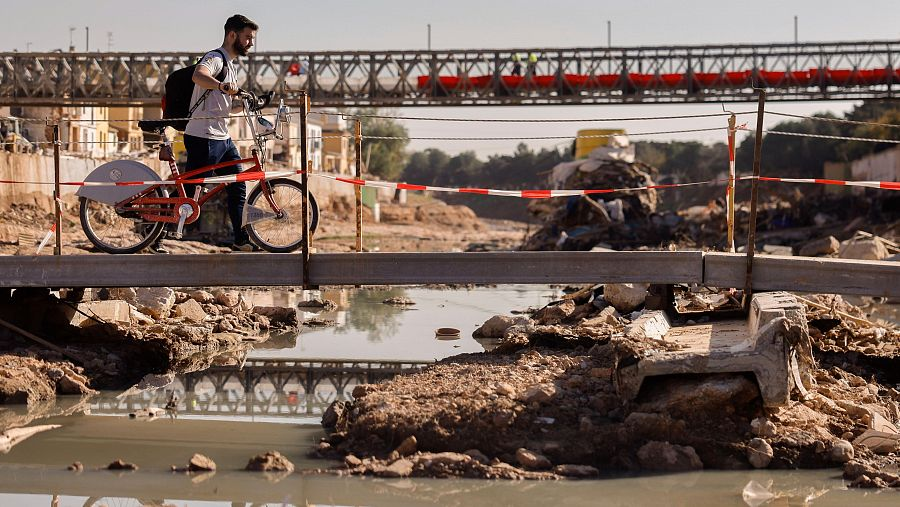
\includegraphics[width=0.8\textwidth]{imagenes/0000_intro1.jpg}
		\caption{Pasarela provisional en la zona del barranco del Poyo en Picanya (Valencia), el 27 de noviembre \cite{0046_infoDANA}}		
		\label{fig:0000_intro1}
	\end{figure} 
	
	\noindent En este contexto, surge la motivación de este Trabajo de Fin de Máster: \textbf{desarrollar un sistema RAG} (Retrieval-Augmented-Generation) (\cite{0003_RAGhowitwork,0003_RAGhowitwork2})  que permita organizar, recuperar y generar información de valor sobre la DANA de Valencia. La elección de este enfoque no es casual, pues las técnicas usadas en un RAG combinan la capacidad de búsqueda eficiente en grandes repositorios de documentos con la generación en lenguaje natural contextualizado y coherente.
	
	\noindent La relevancia social de este trabajo se refuerza por el hecho de que la información utilizada procede de fuentes oficiales, en particular del Boletín Oficial de Estado (BOE) \cite{0048_BOE}. Aunque el BOE constituye la referencia legal sobre ayudas, disposiciones administrativas y medidas de emergencia, su consulta resulta compleja para la mayoría de ciudadanos, más aún en momentos de vulnerabilidad. Una persona afectada por la DANA que necesite conocer qué ayudas solicitar, qué requisitos cumplir o qué plazos respetar se enfrenta a textos jurídicos densos y de difícil navegación. Un sistema RAG aplicado sobre estos documentos permite transformar ese lenguaje administrativo en respuestas claras, comprensibles y accesibles.
	
	\noindent Para hacer efectiva esta idea, el trabajo incluye el \textbf{desarrollo de una interfaz de usuario interactiva}, que permite a cualquier persona formular preguntas en lenguaje natural y recibir respuestas de forma precisa y siempre fundamentadas en la documentación oficial. Esta interfaz no solo es un complemento, sino un componente clave del proyecto, ya que convierte un sistema técnico (como lo es el RAG) en una herramienta práctica con la que cualquier ciudadano, periodista o institución puede interactuar de manera directa. En definitiva, la interfaz actúa como puente entre la complejidad de la inteligencia artificial y la necesidad de simplicidad en la experiencia del usuario final.
	
	\noindent Más allá del desarrollo de una aplicación RAG completa, este TFM también persigue un objetivo de carácter académico y técnico: \textbf{evaluar el sistema RAG} de manera rigurosa mediante métricas específicas. El ámbito de los sistemas RAG es muy dinámico y ofrece múltiples alternativas en cuanto a modelos y algoritmos de recuperación, embeddings y grandes modelos de lenguaje (LLMs). Analizar y comparar diferentes configuraciones resulta fundamental para determinar cuál ofrece el mejor equilibrio entre precisión, coherencia y utilidad práctica. Este segundo objetivo garantiza no solo la validez técnica del trabajo, sino también su capacidad para generar conocimiento transferible a aplicaciones futuras.
	
	\noindent El desarrollo de este proyecto se apoya en la evolución reciente de los modelos de lenguaje (\cite{0005_journeyLLM,0049_tree_evo}), que han alcanzado un nivel de madurez que los convierte en herramientas aptas para aplicaciones de gran impacto social. Muestra de ello es la figura \ref{fig:0000_tree_llm}, donde vemos la gran cantidad de modelos que han ido surgiendo hasta 2023. Los modelos más modernos no solo son capaces de procesar y contextualizar información de manera avanzada, sino que también pueden interactuar con el usuario de manera fluida y natural. Por lo tanto, la integración de estas capacidades en un sistema RAG con interfaz hace posible el diseño de asistentes inteligentes que realmente ayudan en situaciones criticas, consiguiendo a la vez que el ciudadano este informado con fuentes fiables.
	
	\begin{figure}[H]
		\centering
		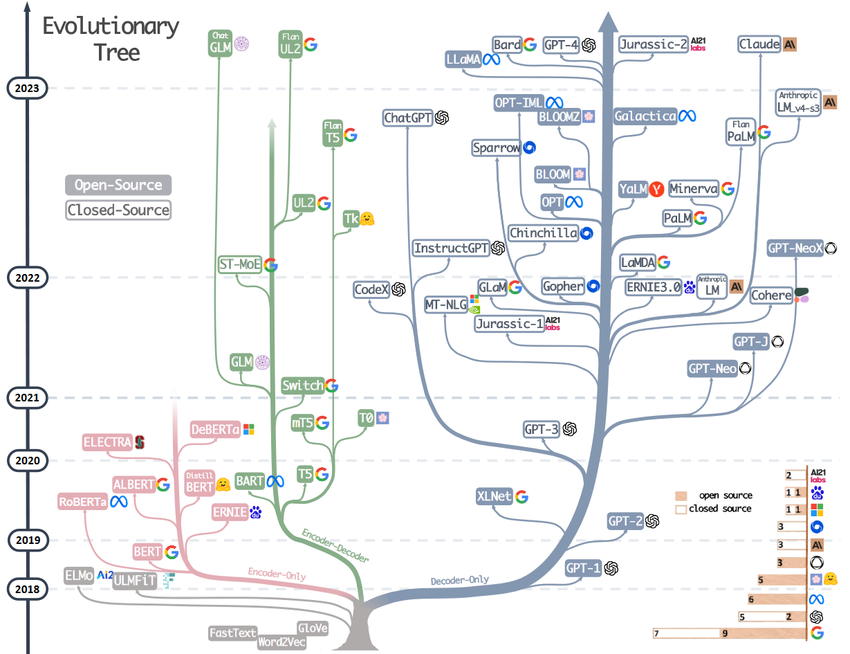
\includegraphics[width=0.8\textwidth]{imagenes/0000_tree_llm.png}
		\caption{Árbol de la evolución de los LLMs modernos \cite{0049_tree_evo}}		
		\label{fig:0000_tree_llm}
	\end{figure} 
	
	\noindent En conjunto, la motivación de este Trabajo de Fin de Máster combina tres vertientes complementarias:
	
	\begin{itemize}
		\item \textbf{Social}, orientada a facilitar el acceso a información oficial a ciudadanos en momentos de crisis ambiental o climática.
		\item \textbf{Práctica}, a través de una interfaz accesible que permite a cualquier usuario interactuar con el sistema RAG sin necesidad de conocimientos previos.
		\item \textbf{Técnica}, centrada en la evaluación comparativa de las diferentes configuraciones que admite un sistema RAG, buscando la máxima eficiencia.
	\end{itemize}
	
	\noindent De este modo, aunque el caso de estudio se centra en la DANA de Valencia de 2024, la metodología y la aplicación desarrollada pueden extrapolarse a otros contextos de crisis. La motivación última es contribuir, desde la investigación universitaria, a un futuro más informado y preparado, en el que la inteligencia artificial actúe como herramienta efectiva para mejorar la vida de la ciudadanía.
	
\section{Objetivos}

	En esta sección comentaremos los dos objetivos definidos para este proyecto: la construcción de un RAG y su evaluación. Describiremos cada uno, desde su justificación hasta su futura implementación.
	
	\noindent El primer objetivo de este trabajo es el desarrollo de un sistema RAG completo, es decir, un sistema que se apoye en información recuperada de una base de conocimiento para generar respuestas más ricas con la ayuda de un modelo de lenguaje. El cometido de nuestro sistema RAG, es el de ayudar a la población a obtener información de cualquier índole (medidas aprobadas, subvenciones, plazos, etc) que esté relacionada con el fenómeno meteorológico DANA, sucedido a finales de 2024.	
	
	\noindent Para este fin, hemos usado documentos del Boletín Oficial de Estado (BOE) relacionados con la DANA para generar nuestra fuente de conocimiento. A partir de aquí, se desarrollará una aplicación con interfaz capaz de recuperar información relevante a la consulta de usuario y de generar una respuesta completa usando esa información. El objetivo es conseguir que nuestro sistema responda con precisión a la duda planteada por la persona en cuestión.
	
	\noindent El segundo objetivo del trabajo, es evaluar el rendimiento de nuestro sistema RAG. Dada la gran cantidad de parámetros ajustables tanto en el modelo de recuperación de información como de elección de modelos de lenguaje para la generación de respuesta, es interesante observar como de distintas son las respuestas ante estos cambios.
	
	\noindent En consecuencia, para la evaluación debemos crear un conjunto de preguntas y respuestas sobre los que aplicar después distintas métricas. Dichas métricas, no son más que \textit{promtps} adaptados que evalúan la precisión, uso de contexto o relevancia de este, en la respuesta generada. Los resultados obtenidos, probando distintas configuraciones en el modelo de recuperación y diferentes modelos de lenguaje, nos indicaran las combinaciones recomendables, o las a evitar.

\section{Estructura de la memoria}

	La estructura de la memoria consta de cinco capítulos finalizando con la bibliografía. El contenido de cada capítulo se describe en la siguiente lista:
	
	\begin{itemize}
		\item \textbf{Capítulo 1. Introducción:} Presenta el proyecto de forma general, explicando la motivación que ha llevado a su realización, los objetivos principales que se persiguen y la organización de la memoria para facilitar su lectura.		
		\item \textbf{Capítulo 2. Estado del Arte:} Revisión de los conceptos teóricos relevantes y descripción de las herramientas, librerías y plataformas empleadas en el desarrollo. Se incluyen además alternativas consideradas, justificando la elección final.		
		\item \textbf{Capítulo 3. Desarrollo del Proyecto:} Exposición del proceso seguido para la construcción de la aplicación RAG, detallando la planificación inicial, la metodología aplicada y las fases de implementación.		
		\item \textbf{Capítulo 4. Evaluación del Proyecto:} Análisis del funcionamiento de la aplicación a partir de métricas y un conjunto de preguntas diseñadas para tal fin. Los resultados se presentan en tablas y gráficas que facilitan su interpretación.		
		\item \textbf{Capítulo 5. Conclusiones y Líneas Futuras:} Recoge las conclusiones generales derivadas del trabajo, así como posibles mejoras y ampliaciones que podrían explorarse en desarrollos posteriores.		
		\item \textbf{Bibliografía:} Relación de las fuentes y referencias consultadas a lo largo de la elaboración del proyecto.
	\end{itemize}
	

\endgroup

\begingroup
\titleformat{\chapter}[block]
{\normalfont\Huge\bfseries\centering} 
{Capítulo \thechapter} 
{0.5em}
{: \LARGE}
[\vspace{1em}\titlerule]

\titlespacing*{\chapter}{0pt}{-60pt}{40pt}

\chapter{Estado del Arte}
\label{cap:2_art}

    En este capítulo explicamos todos los conceptos aparecidos en el proyecto. Mostramos las aplicaciones, tecnologías, herramientas y librerías usadas durante el proceso de desarrollo del mismo, explicando en cada sección las razones y ventajas que tienen sobre otras.

    \section{Generación Aumentada por Recuperación (RAG)}

        La generación aumentada por recuperación o \textbf{RAG} \cite{0003_RAGhowitwork,0003_RAGhowitwork2} por sus siglas en inglés (Retrieval-Augmented Generation), es el concepto principal sobre el que se asienta nuestro proyecto final de máster. Esta técnica complementa la generación de texto que proporcionan los grandes modelos de lenguaje o \textbf{LLMs} (Large Language Models) con información proveniente de datos privados a través de un modelo de recuperación de información, diseñado para buscar en grandes conjuntos de datos o bases de conocimiento. Las respuestas obtenidas de este modo resultan más legibles y más coherentes para el usuario.
        
        \noindent La tecnología RAG ha evolucionado rápidamente en los últimos años, siguiendo distintas etapas ligadas al desarrollo de los grandes modelos de lenguaje (LLM). En sus inicios, surgió junto con la arquitectura \textit{Transformer} y se centró en mejorar los modelos pre-entrenados mediante la incorporación de conocimiento externo. Posteriormente, la aparición de \textit{ChatGPT} marcó un punto de inflexión, al mostrar el potencial del in-context learning y orientar la investigación hacia cómo ofrecer mejor información a los LLM para resolver tareas más complejas y dependientes de conocimiento \cite{gao2024retrievalaugmentedgenerationlargelanguage}.
        
        \noindent Hoy día, la investigación sobre el paradigma RAG continúa evolucionando, tanto que puede ser categorizada en tres etapas \cite{gao2024retrievalaugmentedgenerationlargelanguage} (ver figura \ref{fig:0140_etapasRAG}):
        
        \begin{enumerate}
        	\item \textbf{Naive RAG:} enfoque inicial basado en un esquema tradicional de indexación, recuperación y generación. Es útil, pro presenta problemas de precisión en la recuperación, \textit{alucinaciones} en la generación o redundancia e incoherencia en la integración de información.
        	\item \textbf{Advanced RAG:} surge para intentar superar las limitaciones de la etapa anterior, mejorando tanto indexación (segmentación fina, uso de metadatos, ...) como la post-recuperación (\textit{reranking}). Así reducimos la sobrecarga de información que la damos al LLM y aumentamos la relevancia de esta.
        	\item \textbf{Modular RAG:} representa la etapa más flexible y avanzada. Introduce nuevos módulos y patrones. \textbf{Nota:} esta modalidad no ha investigado en este trabajo.
        \end{enumerate}
        
        \begin{figure}[H]
        	\centering
        	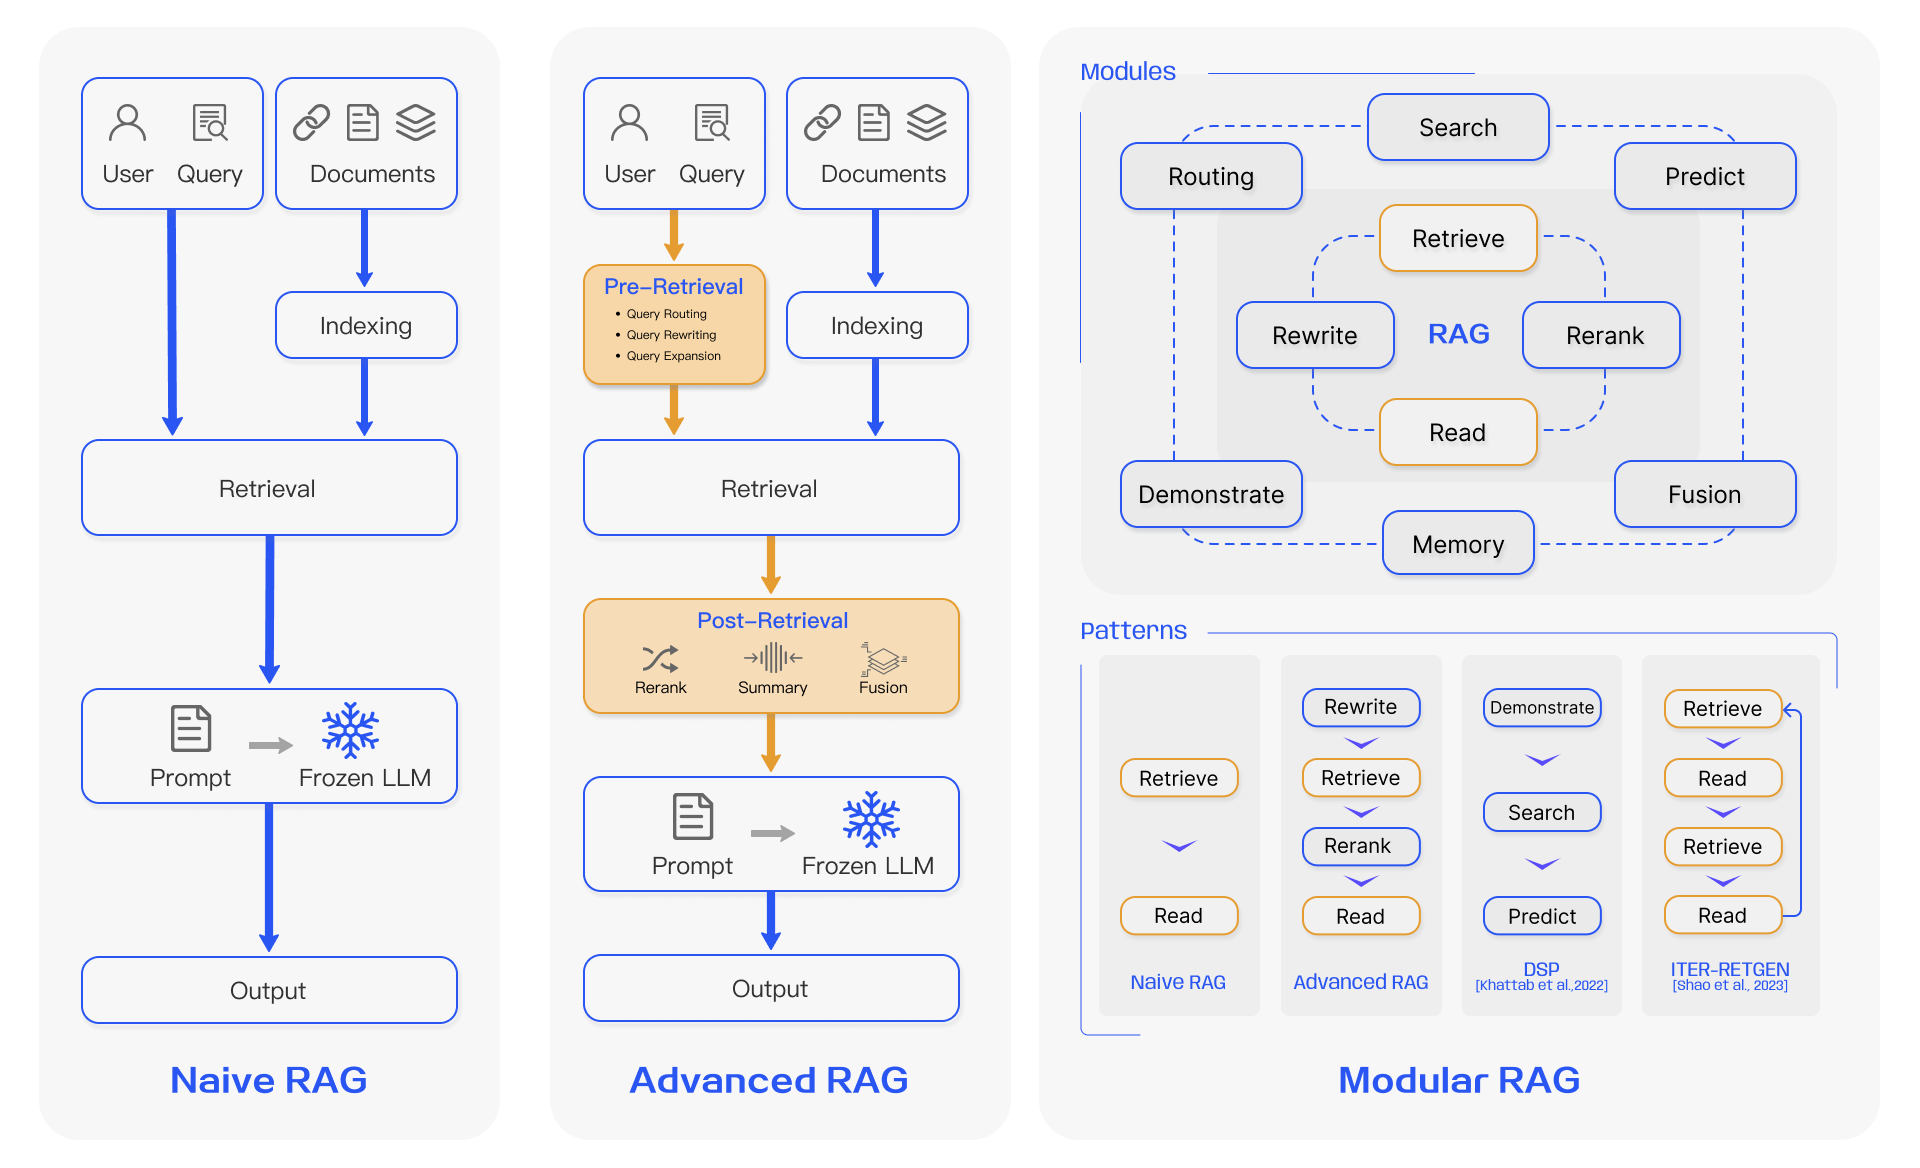
\includegraphics[width=1\textwidth]{imagenes/0140_etapasRAG.png}
        	\caption{Comparación entre los tres paradigma más utilizados de RAG \cite{gao2024retrievalaugmentedgenerationlargelanguage}}		
        	\label{fig:0140_etapasRAG}
        \end{figure} 
        
        \noindent En las siguientes secciones de este apartado iremos desgranando poco a poco más información sobre los conceptos clave LLM-RAG, centrándonos especialmente en el objeto protagonista de este proyecto, el RAG. Mostraremos en que mejora a los LLMs clásicos, explicaremos su funcionamiento y observaremos las ventajas y limitaciones que posee.

        \subsection{Diferencia con los LLMs clásicos}

            Los LLMs tradicionales, como GPT-3 o GPT-4, son modelos pre-entrenados o PLMs (sección \ref{sec:evo_llm}) con grandes conjuntos de datos que generan texto de acuerdo a la información contenida en esos datos \cite{0001_compRAGLLM}. Por lo tanto, su conocimiento esta limitado a la fecha en que fue entrenado, y puede generar respuestas genéricas, no precisas o directamente desfasadas. A este fenómeno se le conoce como \textit{LLM hallucinations} o alucinaciones \cite{0002_LLMhallu}.

            \noindent Optimizar estos modelos para que contengan la información más actualizada y reciente requiere de realizar re-entrenos constantemente, lo que consume muchos recursos y tiempo, por lo que no es una solución adecuada.

            \noindent Los sistemas RAG usan datos recuperados en tiempo real de bases de datos externas en el momento de generar su respuesta al usuario. De esta forma el RAG esta provisto de datos recientes y específicos para el contexto del usuario, sin la necesidad de re-entrenar ningún modelo. La figura \ref{fig:0001-llm-rag} muestra de forma básica este comportamiento.

            \begin{figure}[H]
            	\centering
            	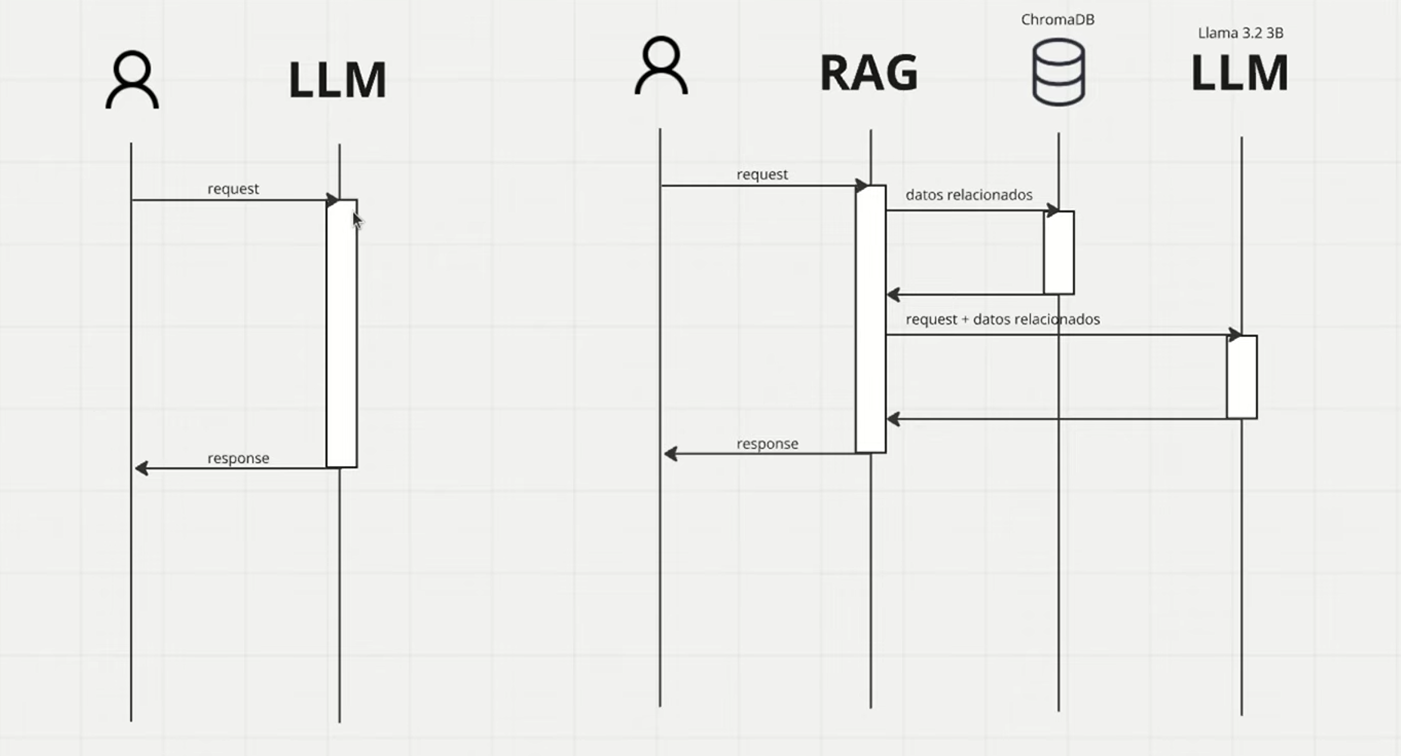
\includegraphics[width=0.8\textwidth]{imagenes/0001-llm_rag.png}
            	\caption{Diferencia básica entre el mecanismo de respuesta de LLM y de RAG. Los LLM responden usando los datos con los que han sido entrenados, mientras que el RAG accede a una base de datos para responder con datos más específicos}		
            	\label{fig:0001-llm-rag}
            \end{figure}  

            \noindent Esta diferencia ayuda al modelo de lenguaje usado por el RAG a adaptar su respuesta al contexto propio del usuario, aportando información relevante y actualizada a la que los LLMs de uso general no tienen acceso.

            \noindent
            
        \subsection{¿Como funciona un RAG?}

            Un sistema RAG se puede comprender como un guión en el que hay que seguir unos pasos para conseguir una respuesta contextualizada y coherente para el usuario \cite{0003_RAGhowitwork,0003_RAGhowitwork2,gao2024retrievalaugmentedgenerationlargelanguage}. Estos pasos se pueden englobar en tres etapas claramente diferenciadas en el proceso de funcionamiento de un RAG, y son las siguientes:

            \subsubsection{Creación del Vector Store}

                El Vector Store es la base de datos que almacenará todo el conocimiento necesario para la lógica de negocio del sistema RAG. Los pasos dentro de esta etapa se pueden resumir en tres: conseguir un conjunto de datos, trocear o separar los datos y almacenar los datos usando modelos de embedding.

                \noindent El conjunto de datos para el RAG es esencial, puesto que en él se reúnen los datos específicos y contextuales que necesitamos y que no poseen los LLMs genéricos. En la mayoría de casos de uso, la información requerida esta contenida en manuales, bases de datos de productos o listas de preguntas frecuentes \cite{0003_RAGhowitwork}.

                \noindent El troceado de datos es el proceso en el cual los datos son transformados en piezas más pequeñas y a su vez más manejables, por ejemplo, dividir un documento de 100 páginas en partes más pequeñas puede ayudar a responder más preguntas a los usuarios. Esto también incrementa la eficiencia del RAG, puesto que el sistema puede obtener rápidamente los trozos de información más relevantes en vez procesar un documento entero.

                \noindent Por último, una vez troceados los datos, necesitamos almacenarlos en nuestra base de datos convertidos en representaciones vectoriales. Esto requiere del uso de los modelos de embedding (sección \ref{sec:embeddings}), que son modelos de lenguaje que transforman el texto de los datos en representaciones numéricas, capturando en ellas las relaciones semánticas del texto durante el proceso (ver figura \ref{fig:0002-rag-db}).

                \begin{figure}[H]
                	\centering
                	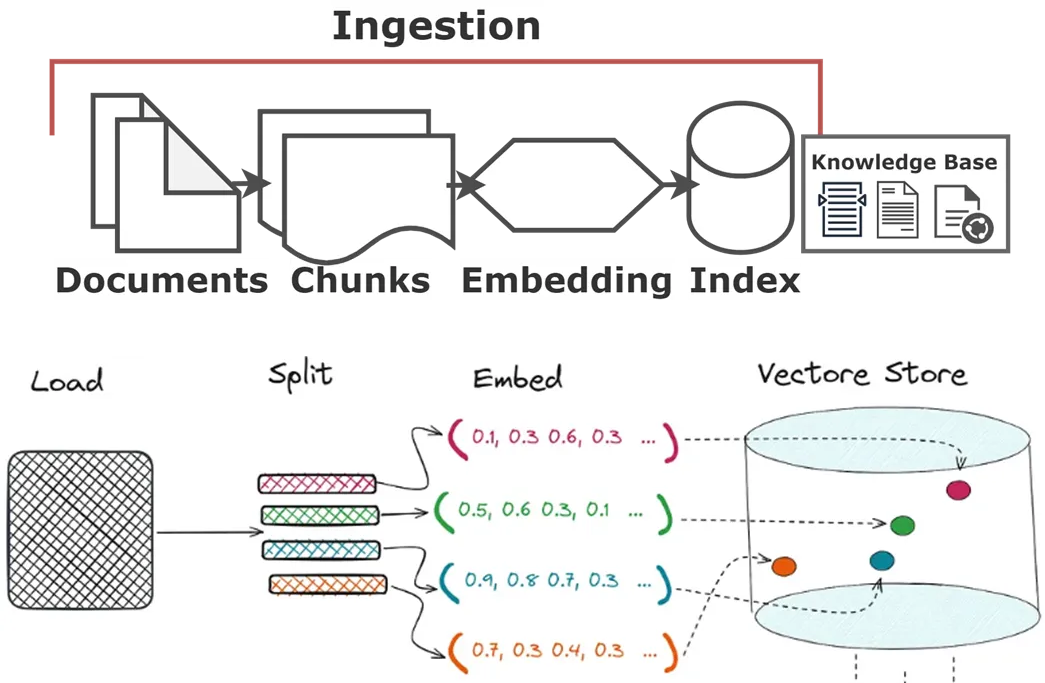
\includegraphics[width=0.6\textwidth]{imagenes/0002-rag-db.png}
                	\caption{Proceso de creación del Vector Store. Se observa todo el proceso: carga, troceado, embedding y almacenamiento \cite{0004_RAGarch}}		
                	\label{fig:0002-rag-db}
                \end{figure}  

            \subsubsection{Recuperación de información}      

                La recuperación de información es la etapa donde entra una consulta al sistema RAG, esta debe ser también vectorizada usando los mismos modelos de embedding que los usados al crear la Vector Store, para garantizar la uniformidad en la respuesta.

                \noindent Una vez vectorizada la consulta el sistema compara ambos embeddings, identifica y retorna las piezas de documentos más parecidas usando medidas de comparación como la similaridad coseno o distancia euclídea entre otras \cite{0003_RAGhowitwork}.La figura \ref{fig:0003-rag-in-action} muestra parte de este proceso.

                \begin{figure}[H]
                    \centering
                    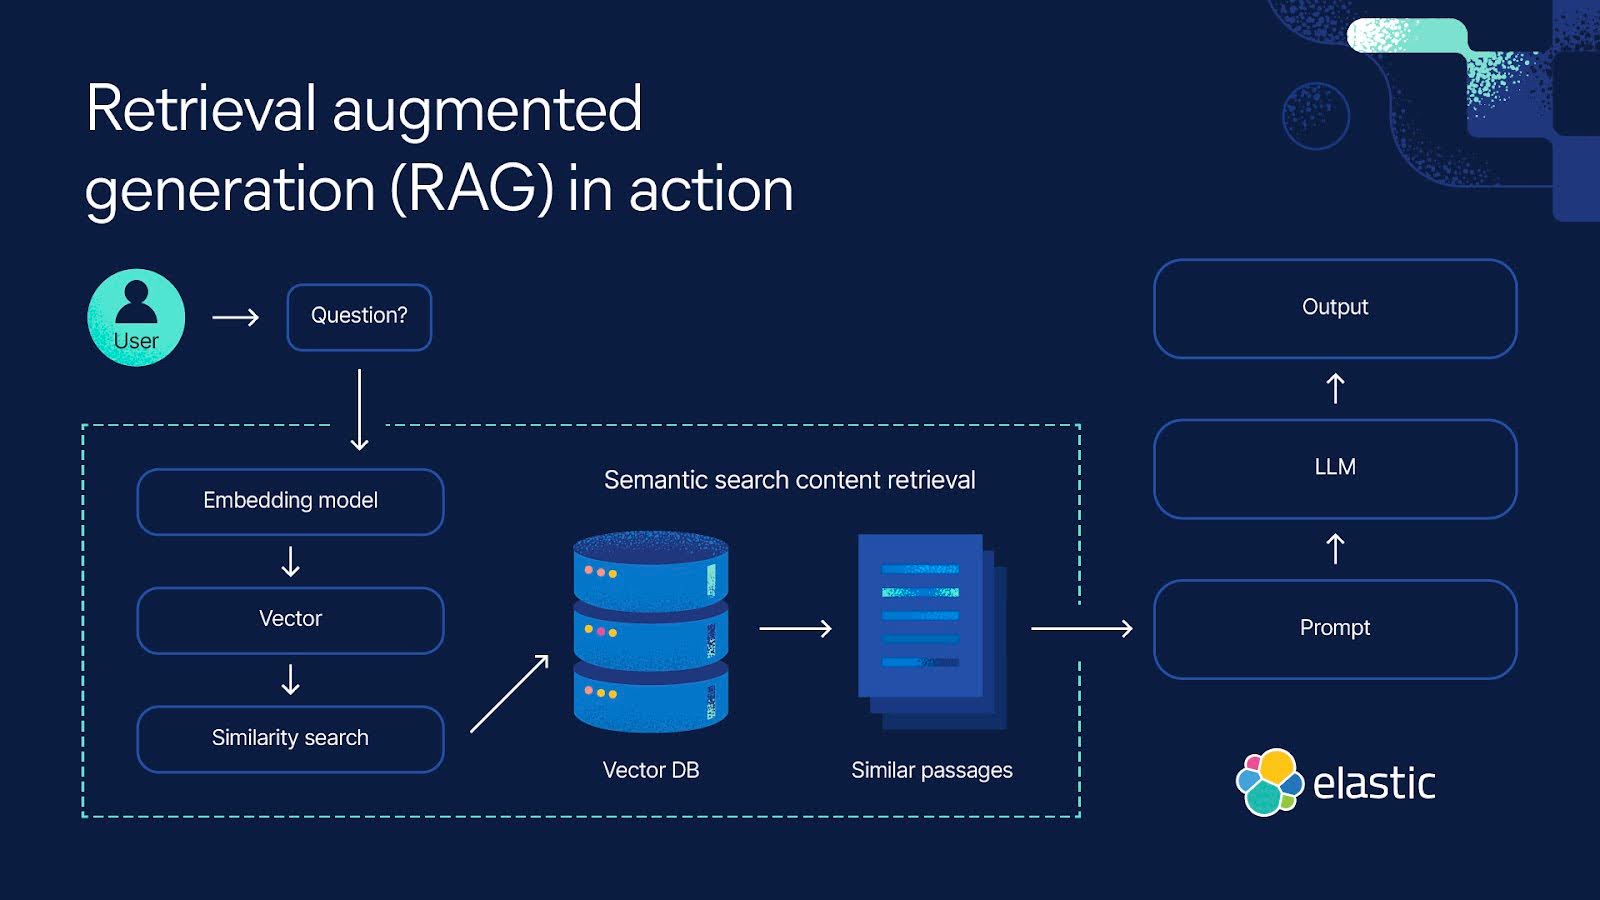
\includegraphics[width=0.8\textwidth]{imagenes/0003-rag-in-action.jpeg}
                    \caption{Fases del proceso de funcionamiento de RAG, se observan las fases de recuperación de información y generación \cite{0003_RAGhowitwork2}}
                    \label{fig:0003-rag-in-action}
                \end{figure}

            \subsubsection{Generación}

                La generación es la etapa que siempre sigue a la recuperación de información. Los documentos recuperados de la consulta inicial son aportados al LLM a través de un prompt \cite{0003_RAGhowitwork2}, que ayuda a generar mediante una serie de instrucciones una respuesta coherente. En la figura \ref{fig:0003-rag-in-action} se puede ver parte de este proceso.

                \noindent Las respuestas obtenidas de esta forma son, en general, más precisas y relevantes dado el contexto, puesto que han sido generadas a partir de los documentos recuperados más relevantes de la base de conocimiento que posee el RAG.
                
        \subsection{Beneficios del RAG}
                       
            Un sistema RAG ofrece múltiples ventajas frente a los modelos de lenguaje que operan de manera aislada. Uno de los principales beneficios es que permite al modelo acceder a información actualizada mediante la integración de fuentes externas, lo que garantiza que las respuestas generadas sean recientes y relevantes para el usuario \cite{0003_RAGhowitwork2}. Esta capacidad de actualización continua resulta clave en entornos donde el conocimiento cambian o evolucionan rápidamente.
                    
            \noindent Otro aspecto destacable es la eficiencia en términos de recursos. Los sistemas basados en RAG suelen requerir menos capacidad de cómputo y almacenamiento, lo que los convierte en una opción más rentable para muchas aplicaciones. Además, al basarse en documentos recuperados durante la consulta, un RAG puede citar sus fuentes y proporcionarlas al usuario, lo que aumenta la transparencia y permite verificar la precisión de las respuestas ofrecidas.
                    
             \noindent En cuanto a la personalización, aunque los modelos de lenguaje ya permiten generar respuestas adaptadas, los RAG va un paso más allá al incorporar mecanismos de recuperación semántica. Esto le permite referenciar contenidos relevantes a partir del contexto específico de la consulta, mejorando la calidad y precisión de las respuestas. Asimismo, frente a preguntas complejas o ambiguas, donde un modelo tradicional podría generar respuestas erróneas o alucinaciones \cite{0002_LLMhallu}, un RAG se apoya en evidencia externa, lo que reduce significativamente este riesgo.
                    
            \noindent Por último, los modelos RAG son altamente versátiles y pueden aplicarse a una amplia gama de tareas de procesamiento de lenguaje natural, como sistemas conversacionales, generación de contenido o recuperación de información, consolidándose así como una herramienta poderosa en el desarrollo de soluciones basadas en inteligencia artificial \cite{0003_RAGhowitwork2}.
        
        \subsection{Desafíos y limitaciones de RAG}
        
            Si bien los sistemas RAG ofrecen ventajas significativas frente a los modelos de lenguaje que operan de forma aislada, también presenta diversos desafíos y limitaciones que deben ser considerados. Uno de los más relevantes es la posibilidad de recuperar información incorrecta o no confiable. Dado que un RAG se basa en fuentes externas para elaborar sus respuestas, una recuperación inadecuada puede derivar en resultados imprecisos o incluso engañosos, afectando la calidad general del sistema.
                    
            \noindent Otro aspecto crítico es el tiempo de búsqueda \cite{0003_RAGhowitwork2}. Al requerir consultas en grandes bases de conocimiento o incluso en la web, el proceso de recuperación puede introducir una latencia considerable, lo que impacta en la experiencia del usuario y en la eficiencia del sistema. Esta limitación exige estrategias de optimización tanto en la indexación como en el diseño de los mecanismos de búsqueda.
                    
            \noindent Además, integrar recuperación y generación en una misma aplicación supone retos importantes en cuanto a diseño e implementación. Es necesario desarrollar soluciones cuidadosas, lo cual puede dificultar la capacitación de los modelos y aumentar la complejidad técnica.
                    
            \noindent La privacidad representa otro desafío relevante \cite{0003_RAGhowitwork2}, especialmente cuando un RAG opera con datos sensibles o confidenciales. En estos casos, es fundamental garantizar el cumplimiento de normativas y políticas de protección de datos, lo que a su vez puede restringir el conjunto de fuentes disponibles.
                    
            \noindent Finalmente, cabe destacar que, por su naturaleza centrada en la recuperación de hechos verificables, un RAG puede mostrar limitaciones a la hora de generar contenido imaginativo o creativo \cite{0003_RAGhowitwork2}. Aunque esto no representa un inconveniente para tareas centradas en la precisión, sí puede reducir su efectividad en aplicaciones donde se espera una mayor capacidad de invención.
        
        \subsection{Tendencias futuras de RAG}
    
            En cuanto al futuro de la generación aumentada por recuperación, las tendencias indican que las tecnologías empleadas para su desarrollo serán cada vez más eficientes y adaptables a una amplia variedad de aplicaciones.
            
            \noindent Los modelos RAG seguirán avanzando hacia una mayor personalización \cite{0003_RAGhowitwork2}, integrando conocimientos específicos del usuario para ofrecer respuestas más precisas y relevantes. Esto será especialmente útil en sistemas de recomendación de contenido y asistentes virtuales, donde la adaptación al perfil del usuario es clave. Además de la personalización, se espera que los usuarios adquieran un mayor control sobre el comportamiento de los modelos, con opciones para ajustar estrategias de búsqueda o modificar la estructura y segmentación del contenido de las bases de datos utilizadas durante la recuperación de información.
            
            \noindent Otra tendencia relevante es el crecimiento en la escalabilidad de los modelos RAG \cite{0003_RAGhowitwork2}, lo que les permitirá manejar un volumen cada vez mayor de datos e interacciones sin comprometer el rendimiento. Asimismo, la integración de RAG con otras técnicas de inteligencia artificial —como el aprendizaje por refuerzo— promete sistemas más versátiles y sensibles al contexto, capaces de gestionar distintos tipos de datos y tareas de forma simultánea.
            
            \noindent Finalmente, a medida que los modelos RAG mejoren en velocidad de recuperación y generación de respuestas \cite{0003_RAGhowitwork2}, será más común su implementación en aplicaciones que demandan baja latencia y tiempos de respuesta en tiempo real, ampliando así su presencia en cualquier entorno.

    \section{Evolución de los LLMs hasta nuestros días}
    \label{sec:evo_llm}

        La forma de extraer información de fuentes de datos textuales ha cambiado ostensiblemente en la última década. Como término, el procesamiento del lenguaje natural ha sobrepasado a la minería de datos como aspecto más importante. Uno de los principales  motivos de este cambio fue la aparición de los modelos de lenguaje, que son utilizados como base para multitud de aplicaciones dedicadas a extraer información valiosa de texto en crudo.

        \noindent Los modelos de lenguaje usan técnicas de aprendizaje automático para predecir palabras mediante probabilidades. Estos modelos aprenden a través de conjuntos de datos textuales, y suelen ser usados para producir textos originales, el reconocimiento de discursos, el reconocimiento óptico de caracteres o el reconocimiento de escritura a mano \cite{0005_journeyLLM,zhao2025surveylargelanguagemodels}.
    
        \noindent La evolución de los modelos de lenguaje ha pasado por cuatro etapas diferenciadas como se pueden observar en la figura \ref{fig:0004-lm-evo}. A continuación, describiremos brevemente estas:
        
        \begin{figure}[H]
            \centering
            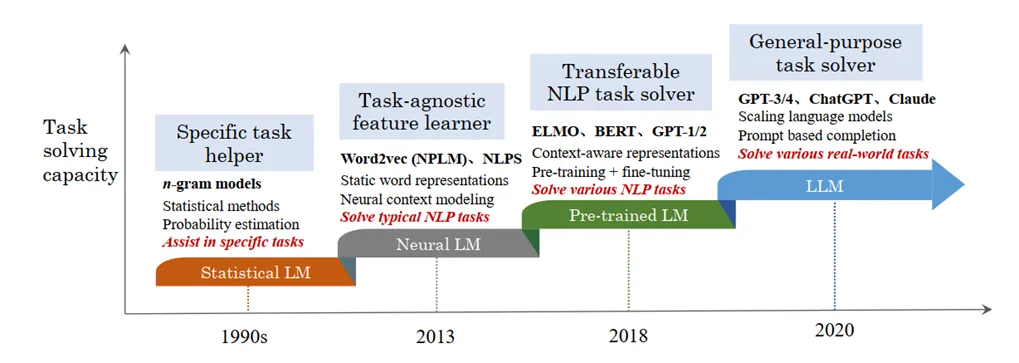
\includegraphics[width=1\textwidth]{imagenes/0004-lm-evo.png}
            \caption{Gráfica de las cuatro etapas en la evolución de los modelos de lenguaje \cite{zhao2025surveylargelanguagemodels}}
            \label{fig:0004-lm-evo}
        \end{figure}
    
        \subsubsection{Modelos de lenguaje estadísticos (SLMs)}
        
            Los modelos de lenguaje estadísticos o SMLs surgieron a partir de el año 1990, e intentaban adivinar la siguiente palabra basándose en las palabras que la precedían. Estos modelos son llamados n-gramas \cite{0005_journeyLLM}: por ejemplo, los bigramas y trigramas predicen según las dos y las tres palabras anteriores respectivamente.
            
            \noindent Mientras los SMLs eran buenos para tareas como la búsqueda de información y la comprensión del lenguaje, tenían un gran inconveniente: la predicción basada en muchas palabras previas, los llamados modelos de gran orden, se complicaba en demasía. La razón principal era la necesidad de estimar un valor exponencial de probabilidades de transición, que en resumen, son valores numéricos comprendidos entre 0 y 1 que representan la probabilidad de que una palabra específica (B) aparezca tras una palabra (A) en una secuencia. 
        
        \subsubsection{Modelos de lenguaje neuronales (NLMs)}
        
            Los SLMs eran buenos al predecir el orden de las palabras, pero fallaban a la hora de entender el lenguaje en profundidad. Los nuevos modelos llamados modelos de lenguaje neuronales o NLMs \cite{0005_journeyLLM} usaban herramientas potentes como redes neuronales, por ejemplo el MLPs (perceptron multicapa) y RNNs (redes neuronales recursivas), que capturaban las relaciones entre palabras. Las modelos como \textit{word2vec} \cite{zhao2025surveylargelanguagemodels} creaban representaciones vectoriales (también denominado modelo de \textit{embeddings}) para cada palabra, ayudando así a a la comprensión de la red de la idea general. 
            
            \noindent Este pequeño avance hacia la compresión del significado de las palabras, no sólo el orden, ha revolucionado como los sistemas procesan el lenguaje, permitiendo a su vez ampliar el rango de tareas en el que son más efectivos, como la generación de texto o la traducción automática de idiomas. Más información sobre modelos de embedding en la sección \ref{sec:embeddings} de esta memoria.
            
        \subsubsection{Modelos de lenguaje pre-entrenados (PLMs)}
        
            Los modelos de lenguaje pre-entrenados o PLMs \cite{0005_journeyLLM}, son modelos que han sido entrenados con un conjunto de datos a través de técnicas de aprendizaje no supervisado. Durante la etapa de pre-entrenamiento, el modelo aprende a comprender y generar texto natural mediante el procesado de grandes cantidades de texto; como por ejemplo: libros, artículos, páginas web, o cualquier contenido de texto disponible en la red. La figura \ref{fig:0005-fine-tuning} muestra un ejemplo de uso para tareas de clasificación de imágenes.
            
            \begin{figure}[H]
                \centering
                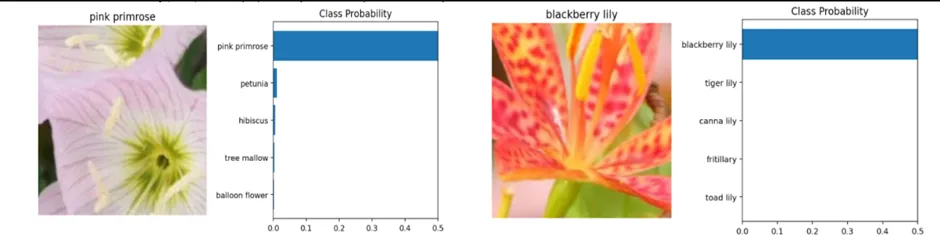
\includegraphics[width=1\textwidth]{imagenes/0005-fine-tuning.png}
                \caption{Fine-tuning en tareas de clasificación de flores usando el modelo pre-entrenado Restnet16 \cite{0005_journeyLLM,zhao2025surveylargelanguagemodels}}
                \label{fig:0005-fine-tuning}
            \end{figure}
            
            \noindent Los modelos pioneros como \textit{ELMo} \cite{zhao2025surveylargelanguagemodels} (Embeddings from Language Models) y \textit{BERT} \cite{zhao2025surveylargelanguagemodels} (Bidirectional Encoder Representations from Transformers) revolucionaron la forma en la que se procesaba el lenguaje natural (NLP) debido a la introducción de palabras representativas del contexto. Estos modelos agregaban al pre-entrenamiento, arquitecturas bidireccionales como \textit{Transformers}.
            
            \noindent Este pre-entrenamiento permitía a los modelos aprender las representaciones numéricas de palabras contextuales, gracias a los \textit{embeddings} (sección \ref{sec:embeddings}) y por consiguiente mejorar significativamente el rendimiento del NLP realizando pequeños ajustes (el llamado \textit{fine-tuning}). Modelos como \textit{GPT-2} \cite{zhao2025surveylargelanguagemodels} (Generative Pre-trained Transformer 2) y \textit{BART} \cite{zhao2025surveylargelanguagemodels} (Bidirectional and Auto-Regressive Transformers) surgieron en consecuencia y abrieron el camino a lo que hoy se conoce como los grandes modelos de lenguaje.

        \subsubsection{Grandes modelos de lenguaje (LLMs)}

            Los grandes modelos de lenguaje son el resultado de la ampliación progresiva de los PLMs. Este crecimiento en tamaño, acompañado del uso de conjuntos de entrenamiento cada vez más extensos y diversos, ha demostrado mejorar significativamente el rendimiento en múltiples tareas. Modelos recientes como \textit{GPT-4} han evidenciado comportamientos distintos respecto a sus predecesores más pequeños, mostrando una mayor capacidad para resolver tareas complejas sin necesidad de entrenamiento adicional.

            \noindent Actualmente, los LLMs están generando un impacto considerable en la comunidad de inteligencia artificial \cite{0005_journeyLLM}. Su desarrollo ha ampliado las expectativas sobre el potencial de estos modelos, hasta el punto de fomentar discusiones sobre una inteligencia artificial con capacidades que podrían igualar o incluso superar el razonamiento humano. Como ejemplo ilustrativo, el modelo \textit{GPT-4.5} ha sido recientemente citado por superar el test de Turing con un 73\% de éxito \cite{0006_ChatGPTuring}. Estas capacidades abren la puerta a aplicaciones que van desde el acceso avanzado al conocimiento y la automatización de tareas complejas, hasta la aceleración de descubrimientos científicos o el impulso económico.
            
            \noindent Una de las características más destacadas de los LLMs es la aparición de capacidades emergentes \cite{0005_journeyLLM}, es decir, habilidades que no estaban presentes en modelos más pequeños y que surgen como resultado del aumento de escala y del refinamiento en el entrenamiento.
            
            \subsubsection{Capacidades emergentes}
            
                El \textit{in-context learning} (aprendizaje en contexto) se refiere a la capacidad del modelo para resolver tareas a partir de ejemplos o instrucciones proporcionadas en la propia entrada del usuario (el prompt), sin necesidad de re-entrenar el modelo. Esta habilidad permite adaptar la respuesta al contexto ofrecido. Por ejemplo:
                
                \noindent \textit{Contexto: ``Eres un asistente virtual especializado en resolver problemas matemáticos."} \\
                \textit{Instrucción: ``Calcula la raíz cuadrada de 25."}
                
                \noindent De forma similar, el seguimiento de instrucciones es posible gracias a que muchos LLMs han sido ajustados utilizando conjuntos de datos formateados como instrucciones en lenguaje natural. Esto permite al modelo generalizar mejor a tareas nuevas, siempre que estén formuladas de manera instructiva.
                
                \noindent Por último, el razonamiento paso a paso hace referencia a la capacidad del modelo para descomponer un problema complejo en pasos más simples, facilitando así su resolución. Al encadenar instrucciones dentro de un \textit{prompt}, se puede guiar al modelo a pensar de forma más estructurada, lo que mejora tanto la precisión como la interpretabilidad de las respuestas generadas.

            \subsubsection{Aplicaciones de un LLM}

                En resumen, los grandes modelos de lenguaje tienen aplicaciones muy variadas que abarcan tanto direcciones de investigación como dominios específicos (ver figura \ref{fig:0006_llm_escena}). 
            
                \begin{figure}[H]
                    \centering
                    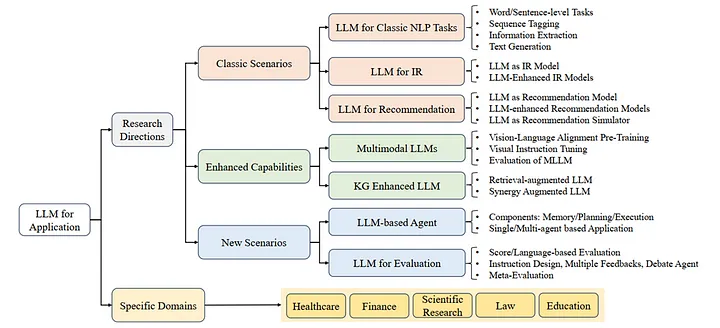
\includegraphics[width=1\textwidth]{imagenes/0006_llm_escena.png}
                    \caption{Esquema de las direcciones de investigación donde podemos usar LLMs \cite{0005_journeyLLM}, \cite{zhao2025surveylargelanguagemodels}}
                    \label{fig:0006_llm_escena}
                \end{figure}
                
                \noindent En el ámbito de las tareas clásicas del procesamiento del lenguaje natural, los LLMs son capaces de abordar actividades como el análisis a nivel de palabra u oración, el etiquetado de secuencias, la extracción de información y la generación de texto. En cuanto a la recuperación de información, estos modelos se utilizan como herramientas de búsqueda por sí mismas o para mejorar modelos existentes, incrementando la precisión y relevancia de los resultados obtenidos. También desempeñan un papel importante en los sistemas de recomendación, ya sea como modelos principales o como complemento de otros sistemas, simulando recomendaciones y ajustándose a las preferencias de los usuarios, como ocurre en plataformas como Netflix y YouTube \cite{0005_journeyLLM}.

                \noindent Los LLMs multi-modales representan otro avance importante, al ser capaces de integrar y procesar información proveniente de distintas modalidades, como texto e imágenes, mejorando así la interacción y comprensión de contenido en diferentes formatos. Asimismo, existen LLMs mejorados con grafos de conocimiento, los cuales incorporan datos estructurados para enriquecer su capacidad de comprensión y generación de contenido con un mayor contexto.
                
                \noindent Además de estas aplicaciones tradicionales, los LLMs se emplean en nuevos escenarios. Uno de ellos son los agentes basados en LLMs, que cuentan con capacidades de memoria, planificación y ejecución, permitiéndoles realizar tareas de manera autónoma y adaptarse a las solicitudes del usuario y al entorno. Otro caso es el uso de LLMs para evaluación, donde se aplican técnicas de evaluación para puntuar modelos o contenidos.
                
                \noindent En cuanto a dominios específicos, los LLMs han demostrado un rendimiento notable. En sanidad, modelos como Med-PaLM \cite{zhao2025surveylargelanguagemodels} han alcanzado un nivel experto en el Examen de Licencia Médica de EE.UU. , siendo aprobados por médicos en la resolución de preguntas médicas. En educación, herramientas como ChatGPT han ayudado a estudiantes a mejorar su rendimiento en asignaturas como seguridad informática, generando o refinando respuestas. En el ámbito legal, GPT-4 obtuvo una puntuación dentro del 10\% superior en un examen de acceso a la abogacía simulado, evidenciando su capacidad para la interpretación legal y el razonamiento. En finanzas, BloombergGPT \cite{zhao2025surveylargelanguagemodels} \cite{wu2023bloomberggptlargelanguagemodel} demostró un rendimiento destacado en múltiples tareas financieras, sin perder competitividad en tareas de propósito general. Por último, en la investigación científica, los LLMs han sido utilizados en distintas fases del proceso científico, incluyendo la revisión bibliográfica, la generación de hipótesis, el análisis de datos y la redacción de artículos. 

            \subsection{LLMs usados en el proyecto}
            \label{sec:cap2_llms_usados}

                Durante la realización del proyecto, hemos probado varios modelos de lenguaje, incluyendo modelos locales y externos. Los modelos seleccionados finalmente han sido tres, diferenciando las tres estrategias que podemos usar a la hora de usar un LLM, es decir: un modelo local, un modelo gratuito externo y un modelo externo de pago.

                \noindent En los siguientes apartados se explican con más detenimiento los modelos elegidos y las plataformas en los que están disponibles.

                \subsubsection{Llama 3.2}

                    Llama 3.2 \cite{0037_llama32} es modelo de lenguaje multilingüe perteneciente a Meta. Es una colección de modelos pre-entrenados diseñados para seguir instrucciones, con un tamaño de 1 a 3 billones de parámetros (1B y 3B). La versión usada en el proyecto es la 3B.

                    \noindent El modelo está optimizado para mantener conversaciones en varios idiomas, incluyendo tareas como la realización de agentes de búsqueda y resúmenes.
            
                    \begin{figure}[H]
                        \centering
                        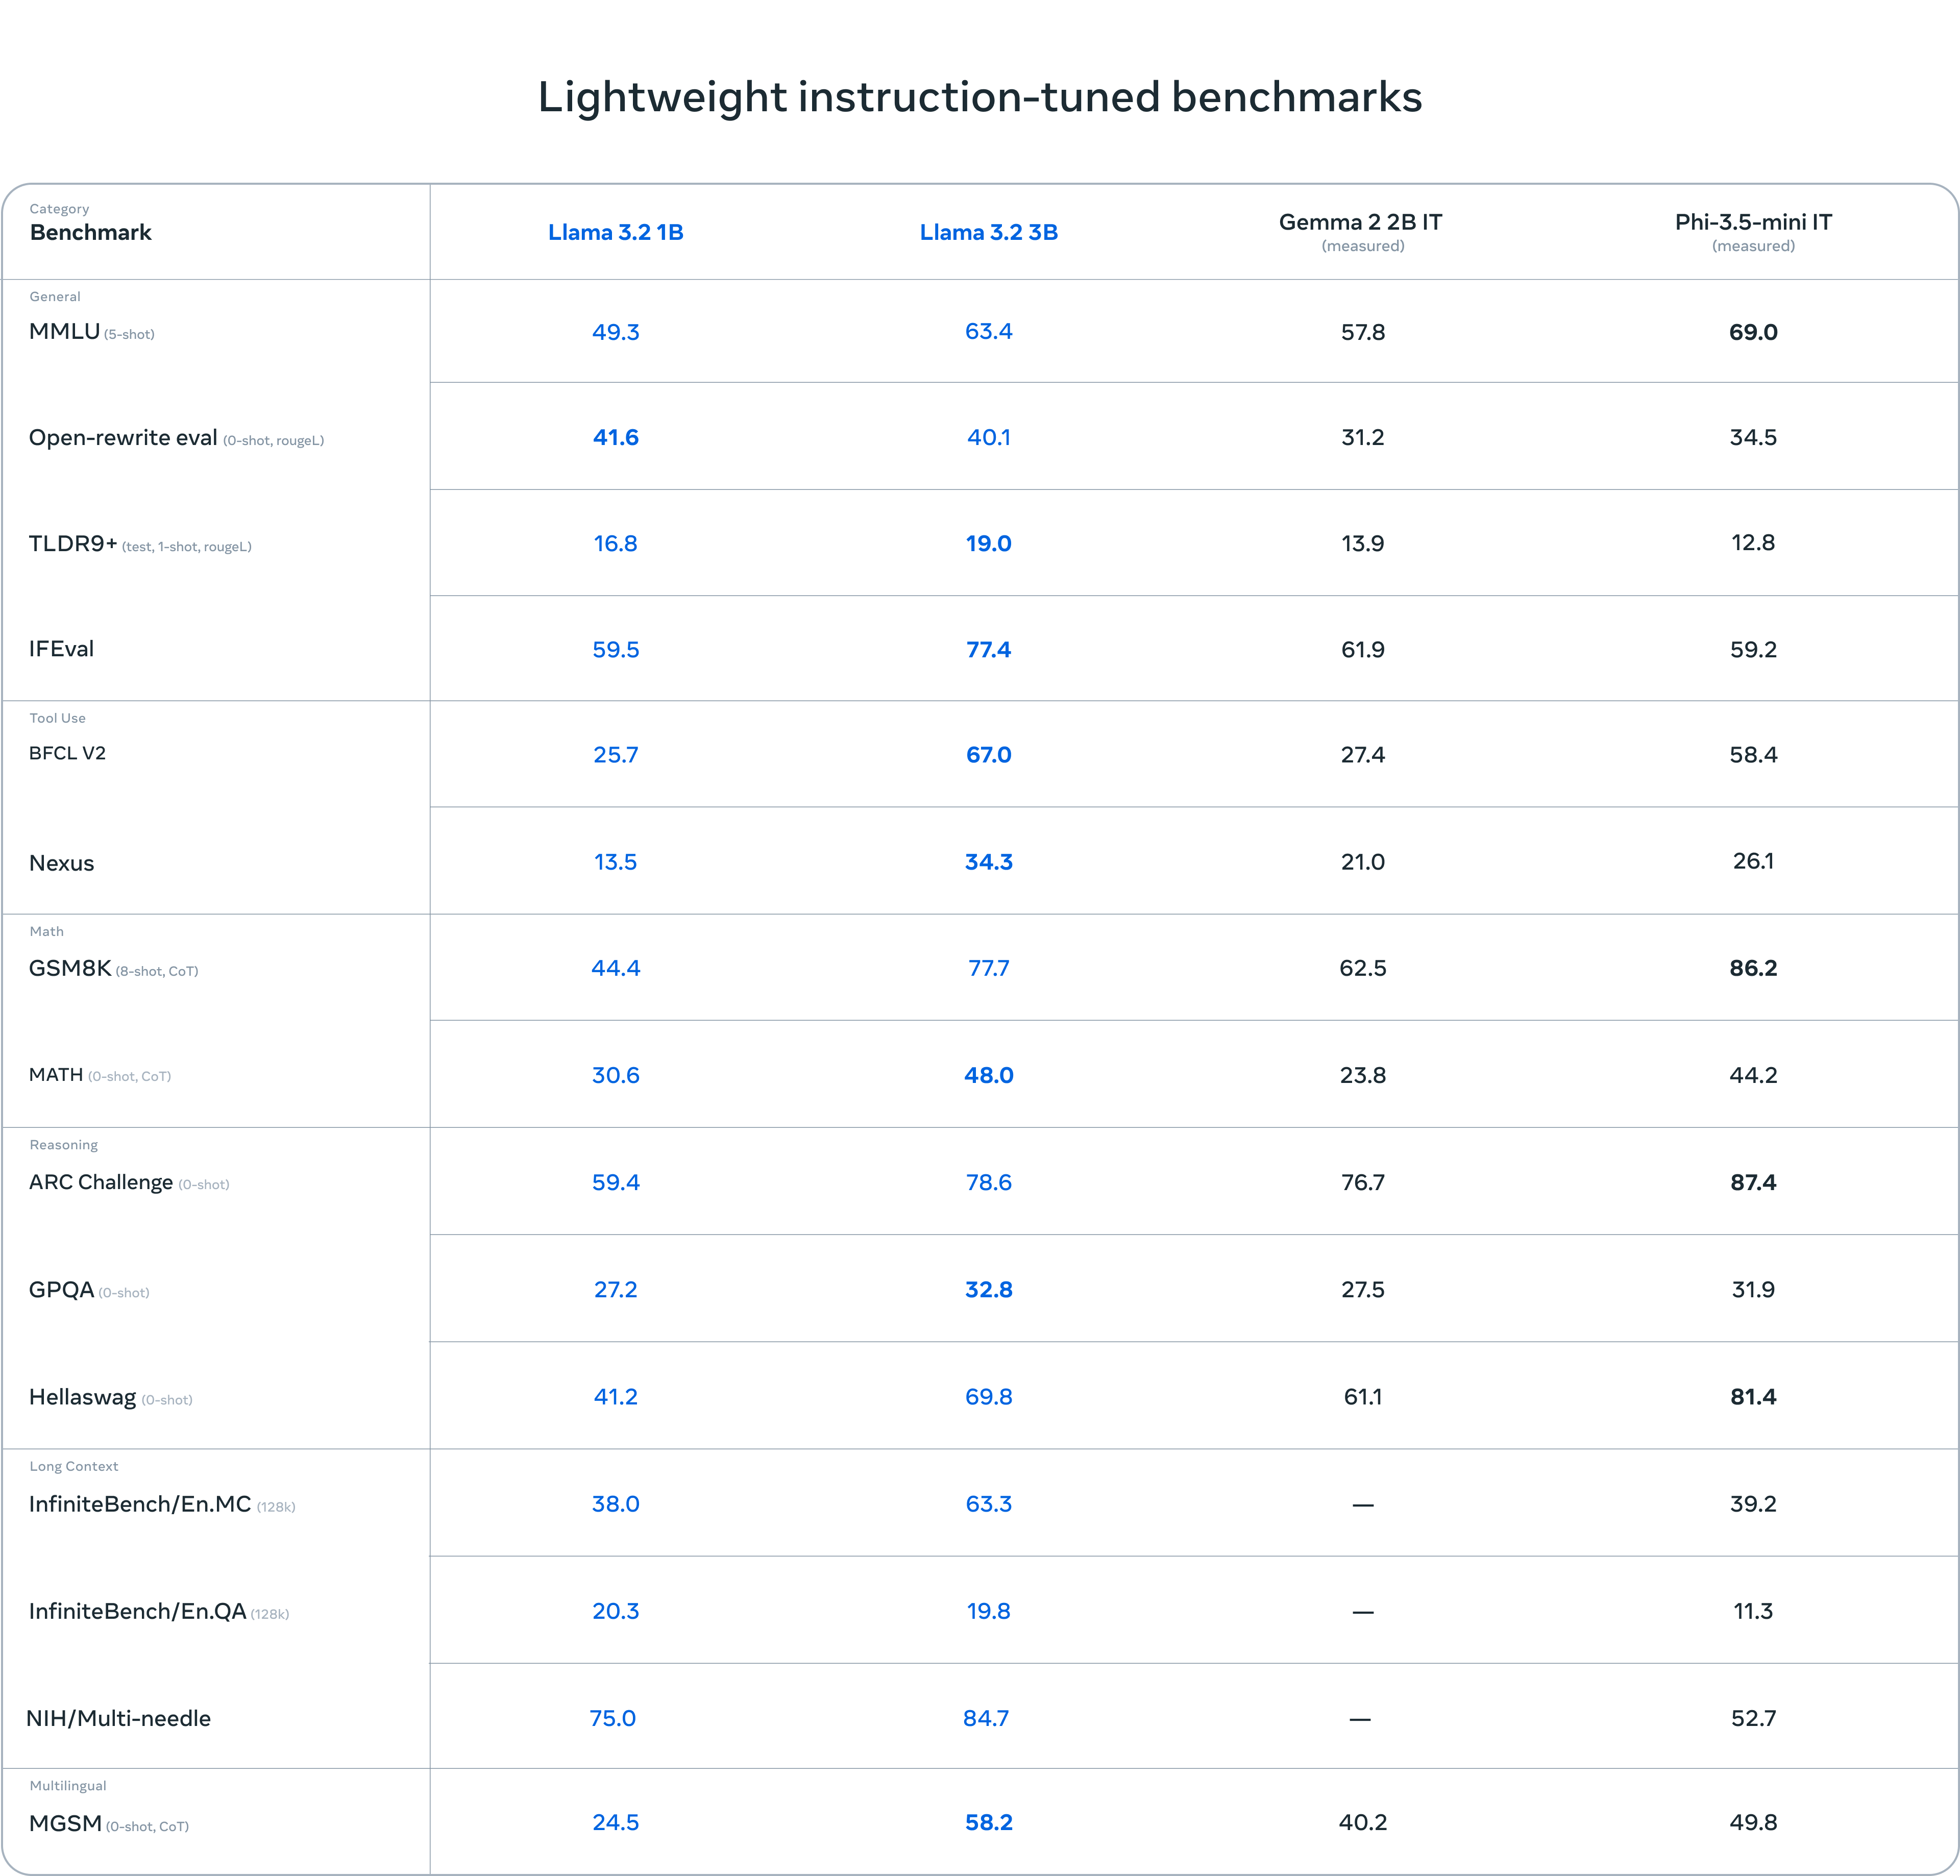
\includegraphics[width=1\textwidth]{imagenes/0090_llama32.png}
                        \caption{Tabla comparativa del modelo Llama 3.2 en diferentes benchmarks \cite{0037_llama32}}
                        \label{fig:0090_llama32}
                    \end{figure}

                    \noindent La plataforma donde esta disponible una versión de este modelo es Ollama (ver sección \ref{sec:ollama}). Es la opción que usaremos en el proyecto como base de pruebas de un modelo local, ya que la plataforma Ollama permite la descarga de multitud de modelo gratuitos.
                    
                \subsubsection{Mistral Small 3.2}

                    Mistral Small 3.2 \cite{0038_mistralsmall32} es la última actualización disponible del modelo Mistral Small. Este modelo mejora al anterior (Mistral Small 3.1 \cite{0039_mistralsmall31}) a la hora de dar respuestas precisas a instrucciones, generar menos texto repetitivo o generaciones infinitas.

                    \noindent El modelo Mistral Small 3.2 cuenta con un tamaño de 24 billones de parámetros (24B), algo considerable para ser usado localmente. Mistral AI ofrece este y otros modelos de forma gratuita a través de su API (con ciertas restricciones ratio/preguntas), por esa razón, es el modelo escogido para realizar las pruebas con un modelo externo gratuito.

                    \noindent \textbf{Nota:} La siguiente figura muestra el rendimiento del modelo 3.1. Mistral Small 3.2 es relativamente moderno (junio de 2025), y a día de hoy, no disponemos de un blog/página oficial que informe sobre su rendimiento actual.
            
                    \begin{figure}[H]
                        \centering
                        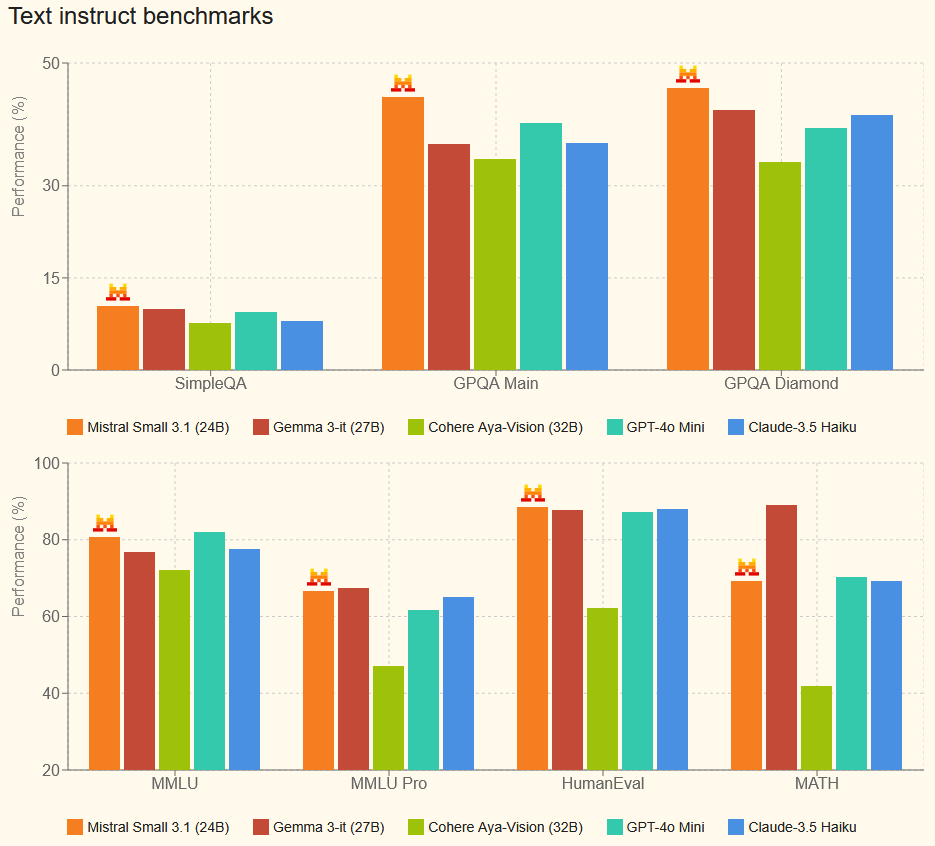
\includegraphics[width=.8\textwidth]{imagenes/0091_mistralsmall31.png}
                        \caption{Tabla comparativa del modelo Mistral Small 3.1 en diferentes benchmarks \cite{0039_mistralsmall31}}
                        \label{fig:0091_mistralsmall31}
                    \end{figure}

                \subsubsection{GPT-4.1}

                    El conjunto de modelos GPT-4.1 \cite{0043_gpt41} esta disponible en tres tamaños: GPT-4.1, GPT-4.1 Mini y GPT-4.1 Nano. Están destinados a programadores que necesitan un mayor rendimiento, un contexto más amplio y un seguimiento de las instrucciones más predecible. Cada modelo admite hasta 1 millón de tokens de contexto, un salto apreciable dado que los modelos anteriores permitían un tamaño de contexto de 128 mil.
                    
                    \noindent GPT-4.1 mejora las capacidades de GPT-4o, manteniendo la latencia más o menos en el mismo rango. En la práctica, significa que podemos obtener mejor rendimiento sin pagar un coste en capacidad de respuesta (ver figura \ref{fig:0121_gptprecios} para ver los precios). En la siguiente figura, GPT-4.1 adelanta en inteligencia a GPT-4o manteniendo una velocidad similar. De igual manera, la versión \textit{mini} es más inteligente siendo un poco más lenta.
                    
                    \begin{figure}[H]
                    	\centering
                    	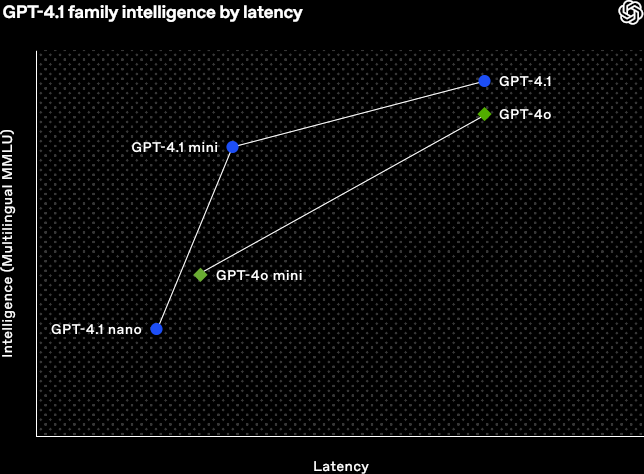
\includegraphics[width=.8\textwidth]{imagenes/0120_gpt41.png}
                    	\caption{Rendimiento del conjunto de modelos GPT-4.1 \cite{0043_gpt41_2}}
                    	\label{fig:0120_gpt41}
                    \end{figure}
                    
                    \begin{figure}[H]
                    	\centering
                    	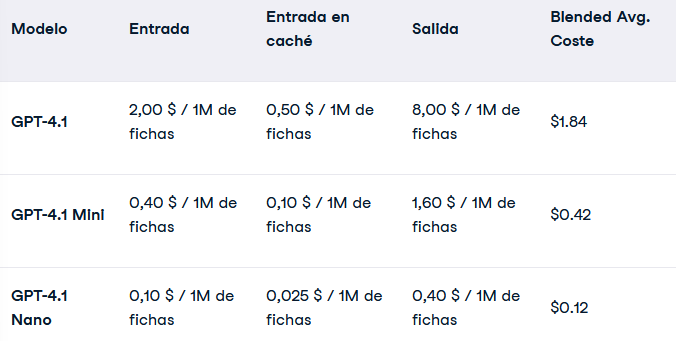
\includegraphics[width=.8\textwidth]{imagenes/0121_gptprecios.png}
                    	\caption{Precio de los modelos GPT-4.1 \cite{0043_gpt41_2}}
                    	\label{fig:0121_gptprecios}
                    \end{figure}
                    
                    \noindent El modelo GPT-4.1 es el escogido realizar las pruebas, para lo cual necesitaremos conseguir una de las claves API disponibles en la plataforma de OpenAI. Siempre que tengamos créditos en la cuenta podemos acceder al modelo, por lo que hay que tener en cuenta este factor. Con este modelo de pago, ya tenemos todos los modelos de los que queremos evaluar su rendimiento en nuestro proyecto.


    \section{Modelos de Embedding}
    \label{sec:embeddings}

        Los modelos de embedding son la parte esencial en el modelo de recuperación de información de un sistema RAG, ya que permiten transformar datos complejos como texto, imágenes o audio \cite{0007_Embeddings}; en representaciones vectoriales densas y de baja dimensión. Estas representaciones conservan relaciones semánticas relevantes y resultan mucho más manejables para recuperar documentos relevantes dada una consulta de usuario.
    
        \begin{figure}[H]
            \centering
            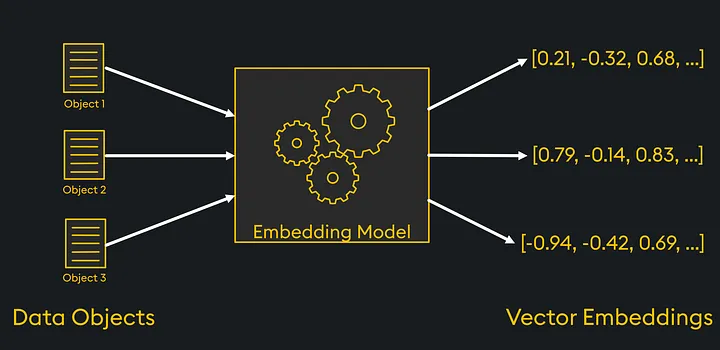
\includegraphics[width=0.7\textwidth]{imagenes/0007-ej-embeddings.png}
            \caption{Ejemplo básico de funcionamiento de un modelo de embeddings \cite{0007_Embeddings}. Recibe objetos de datos, que pueden ser de todo tipo, y los transforma en una representación vectorial}
            \label{fig:0007-ej-embeddings}
        \end{figure}
            
        \noindent Por otra parte, los embeddings también son una pieza fundamental en multitud de técnicas de aprendizaje automático. Los vectores generados pueden emplearse en tareas como clasificación, agrupamiento (clustering), recomendación o recuperación de información, etc. 
        
        \noindent Gracias a su versatilidad, los modelos de embedding se utilizan en una amplia variedad de aplicaciones del mundo real. En sistemas de análisis de sentimientos, permiten identificar matices emocionales en el texto a partir de la representación semántica de las palabras. En sistemas de recomendación, se emplean para medir similitudes entre usuarios y productos, ofreciendo sugerencias personalizadas. En tareas de respuesta automática a preguntas, los embeddings permiten emparejar preguntas y respuestas en función de su similitud semántica, facilitando la recuperación de la respuesta más adecuada. Finalmente, debido a que estos modelos pueden representar palabras y frases en múltiples idiomas dentro de un mismo espacio vectorial, también resultan especialmente útiles en tareas de traducción automática, donde es posible identificar significados equivalentes entre lenguas diferentes \cite{0007_Embeddings}.
            
        \noindent En resumen, los modelos embeddings son una herramienta clave para representar datos de forma compacta y significativa, lo que habilita una gran variedad de aplicaciones en el campo del aprendizaje automático y el procesamiento del lenguaje natural.

        \noindent En las siguientes sub-secciones hablaremos de los modelos de embeddings utilizados en nuestro sistema RAG.

        \subsection{Nomic Embed (nomic-embed-text)}

            \textbf{Nomic Embed} \cite{0024_nomic} es un modelo avanzado de embedding de texto desarrollado por \textbf{Nomic}, diseñado para ofrecer una capacidad excepcional en tareas tanto de corto como de largo contexto. Este modelo sobresale frente a alternativas como \textit{Ada-002} o \textit{text-embedding-3-small} de OpenAI (figura \ref{fig:0048_nomic}), gracias a su enfoque en la accesibilidad y auditabilidad completa del modelo.
    
            \begin{figure}[H]
                \centering
                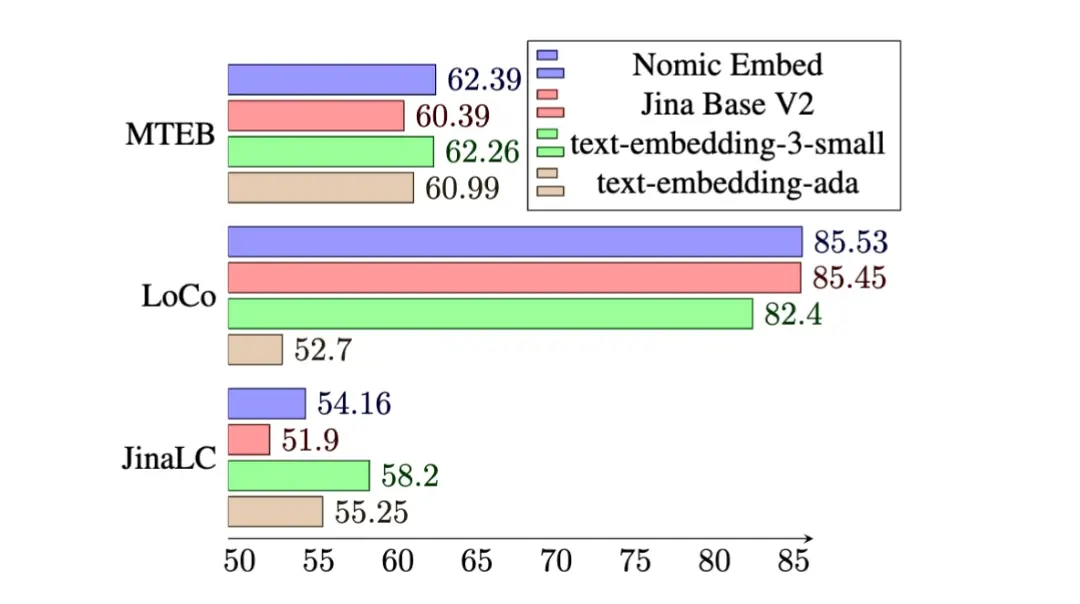
\includegraphics[width=0.8\textwidth]{imagenes/0048_nomic.png}
                \caption{Rendimiento comparativo de Nomic Embed y otros modelos en distintos benchmarks \cite{0024_nomic}}
                \label{fig:0048_nomic}
            \end{figure}

            \noindent Las características destacadas de este modelo \cite{0024_nomic} se pueden resumir en: código abierto y rendimiento. Nomic Embed se distingue por su enfoque abierto completamente abierto, incluyendo datos de entrenamiento, código de entrenamiento y modelos bajo licencia Apache2.

            \noindent Evaluado en benchmarks como \textit{MTEB} y \textit{LoCo} (figura \ref{fig:0048_nomic}), Nomic Embed supera a modelos líderes en tareas de largo contexto, demostrando consistencia y superioridad en entornos supervisados y no supervisados.       

            \noindent En resumen, nomic Embed se posiciona como una opción muy recomendable para proyectos que buscan integrar modelos de embedding de texto avanzados y completamente auditables.

        \subsection{BGE-M3}        

            BGE-M3 \cite{0025_bge-m3} es otro modelo de embedding de texto basado en la arquitectura \textit{XLM-RoBERTa}, diseñado para ser altamente versátil en diversos escenarios de recuperación de información. Su nombre proviene de sus tres capacidades:

            \begin{itemize}
                \item \textbf{Multi-funcionalidad}: BGE-M3 es capaz de realizar de manera simultánea recuperación densa, recuperación con multiples vectores y recuperación dispersa, ampliando significateivamente su rango de aplicación.
                \item \textbf{Multilingüe}: Este modelo ofrece soporte para más de cien idiomas, lo que lo convierte en una herramienta eficaz en contextos multilingües y de alcance global.
                \item \textbf{Multi-granularidad}: Puede procesar texto con distintos niveles de granularidad, desde frases cortas hasta documentos de hasta 8192 tokens de longitud.
            \end{itemize}
    
            \begin{figure}[H]
                \centering
                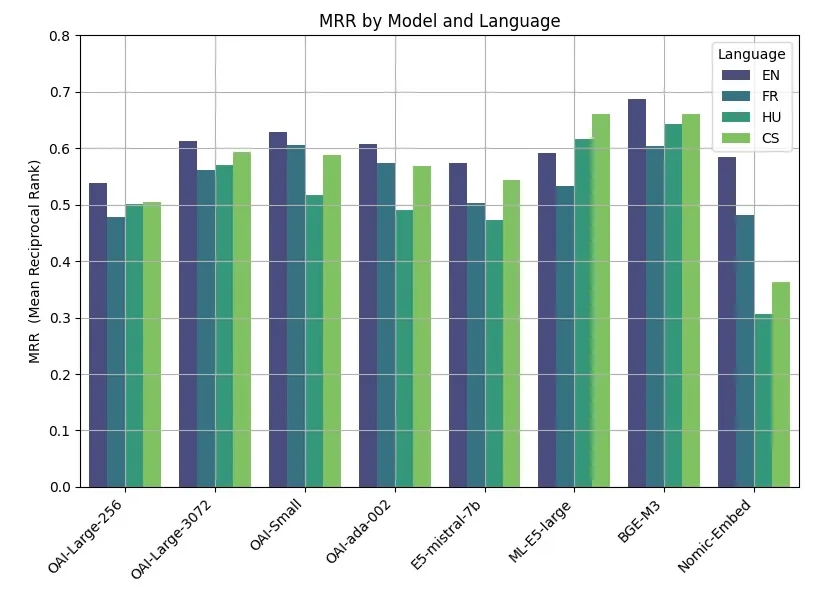
\includegraphics[width=0.8\textwidth]{imagenes/0049_bge-m3.png}
                \caption{Rendimiento comparativo del modelo bge-m3 con otros modelos \cite{0025_bge-m3}}
                \label{fig:0049_bge-m3}
            \end{figure}

            \noindent Definitivamente, BGE-M3 resulta ideal para sistemas de búsqueda semántica multilingüe y cualquier entorno donde se requiera una compresión profunda del texto en múltiples idiomas. Su enfoque multifuncional representa un avance significativo en el desarrollo de modelos de embedding flexibles, escalables y multilingües.

        \subsection{Artic Embed 2.0 (snowflake-arctic-embed2}

            El modelo Artic Embed 2.0 \cite{0026_snowflake}, desarrollado por Snowflake, representa la nueva iteración en sus modelos de embedding \textit{frontier}. Esta nueva versión incorpora soporte multilingüe sin comprometer su rendimiento o escalabilidad.
    
            \begin{figure}[H]
                \centering
                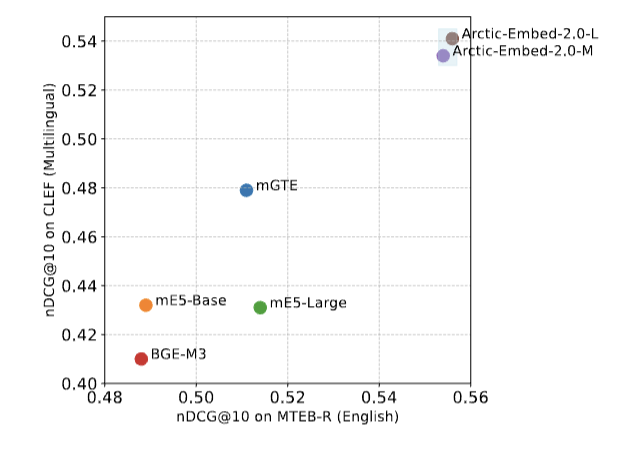
\includegraphics[width=0.8\textwidth]{imagenes/0050_snowflake.png}
                \caption{Métricas obtenidas por los modelos de Artic Embed en comparación con otros, usando el benchmark MTEB-R en inglés. \cite{0026_snowflake}}
                \label{fig:0050_snowflake}
            \end{figure}

            \noindent Artic Embed 2.0 logra resultados altos en tareas de recuperación semántica tanto en inglés como en otros idiomas europeos, demostrando una notable capacidad de generalización incluso en lenguas no vistas durante el entrenamiento.

            \noindent Snowflake ha diseñado este modelo pensando el entornos de alta demanda, ofreciendo latencias de 10ms por consulta. Incluye una compresión eficiente (MRL, Matryoshka Representation Learning) que permite búsquedas rápidas y económicas en grandes conjuntos de datos.
            
            \noindent Este modelo se distribuye bajo una licencia de uso Apache 2.0, permitiendo su libre uso.

            \noindent En resumen, Snowflake ofrece un modelo de embedding con soporte multilenguaje, capacidad de compresión y orientado a entornos empresariales.

        \subsection{Jina Embeddings v2 Base ES ( jina-embeddings-v2-base-es)}

            El modelo de embedding bilingüe español-inglés \textit{jina-embeddings-v2-base-es} \cite{0027_jina}, desarrollado por Jina AI, está diseñado para aplicaciones que requieren representaciones semánticas robustas en cualquiera de estos dos idiomas. 

            \noindent Basado en una arquitectura BERT (JinaBERT), este modelo esta pensado para ofrecer un alto rendimiento en aplicaciones monolingües y bilingües ya que ha sido entrenado específicamente para admitir entradas de español e inglés sin sesgo.

            \noindent Además, su tamaño se ubica entre los más ligeros entre los embeddings multilingües disponibles, facilitando su implementación en entornos con recursos limitados.

            \noindent Por último, puede integrarse fácilmente vía Python a través de Ollama, y es apto para sistemas RAG según pruebas recientes con LlamaIndex (ver figura \ref{fig:0051_jina}).             
    
            \begin{figure}[H]
                \centering
                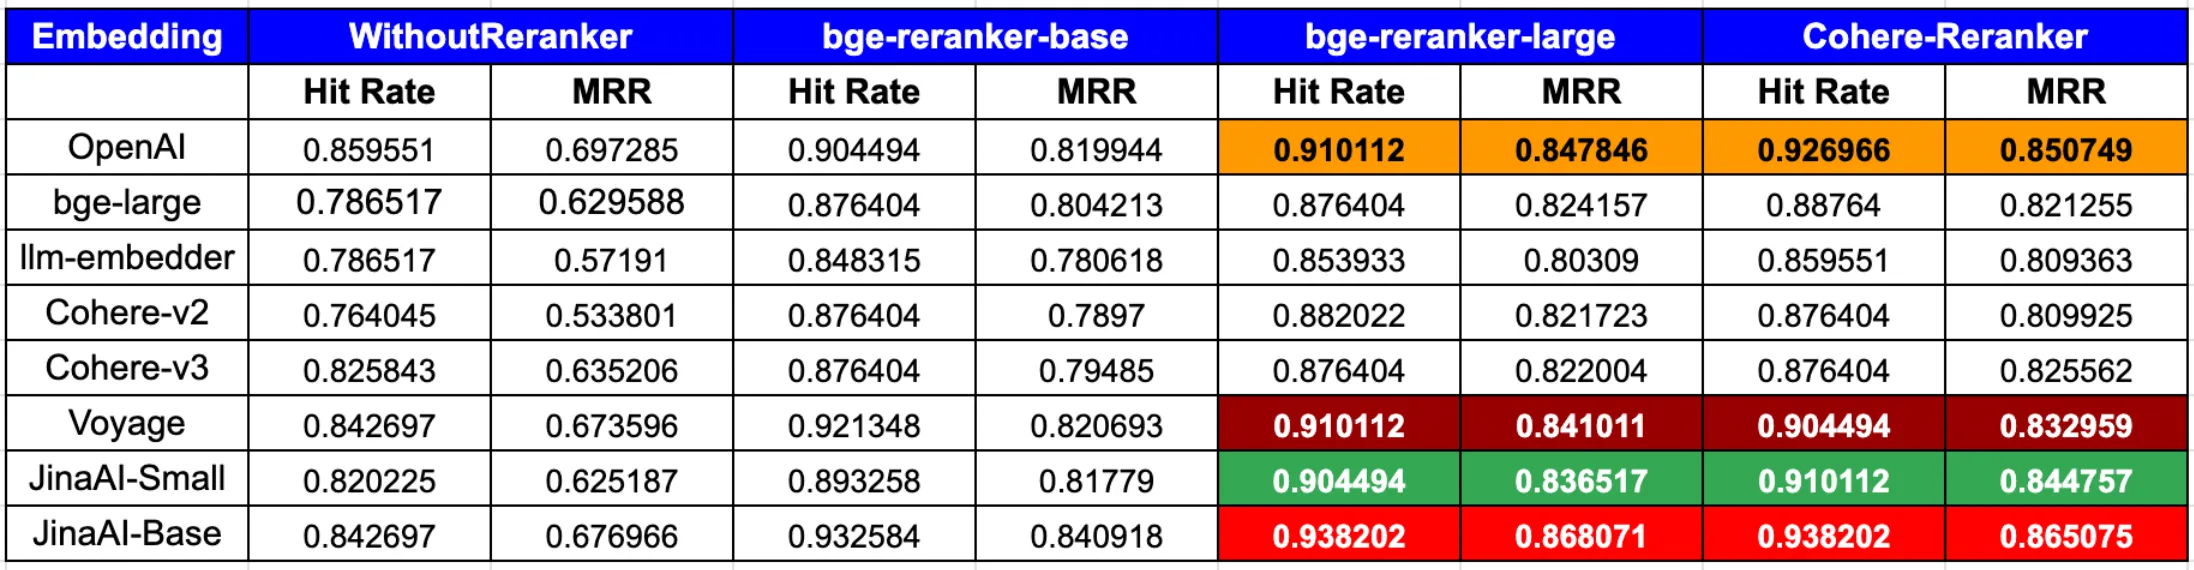
\includegraphics[width=1\textwidth]{imagenes/0051_jina.png}
                \caption{Comparación de varios modelos de embedding con JINA. \cite{0027_jina}}
                \label{fig:0051_jina}
            \end{figure}

        \subsection{Text Embedding 3 (text-embedding-3-small)}

            El modelo \textit{text-embedding-3-small} es una versión mejorada y eficiente del modelo de embedding anterior \textit{text-embedding-ada-002}, ambos pertenecientes a \textbf{OpenAI} \cite{0040_openai_embed}.                  

            \noindent Como se puede observar en la figura \ref{fig:0097_te3s}, la puntuación media en una prueba comparativa de uso común para la recuperación en varias lenguas (MIRACL) aumento de un 31,4\% hasta el 44\%, mientras que la puntuación media para tareas en inglés (MTEB) aumento del 61\% hasta el 62,3\%.
    
            \begin{figure}[H]
                \centering
                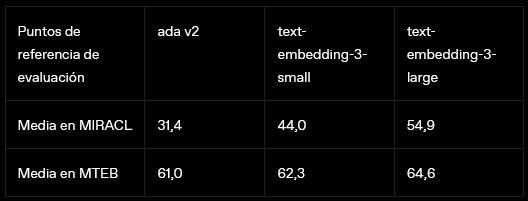
\includegraphics[width=.7\textwidth]{imagenes/0097_te3s.png}
                \caption{Evaluaciones de los modelos de embedding de OpenAI \cite{0040_openai_embed}}
                \label{fig:0097_te3s}
            \end{figure}

            \noindent El precio de uso también se ha reducido al ser un modelo más eficiente que el anterior, casi cinco veces.

            \noindent Este modelo ha sido entrenado con una técnica que permite a los desarrolladores equilibrar el rendimiento y costes al utilizar las integraciones, podemos acortarlas sin perder sus propiedades de representación de conceptos (ver figura \ref{fig:0098_te3s_2}).
            
            \begin{figure}[H]
            	\centering
            	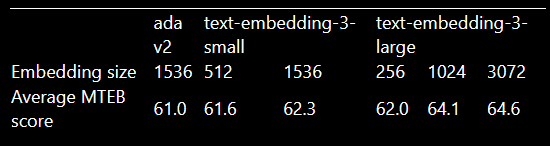
\includegraphics[width=.7\textwidth]{imagenes/0098_te3s_2.png}
            	\caption{Evaluaciones de los modelos de embedding de OpenAI con distintos tamaños \cite{0040_openai_embed}}
            	\label{fig:0098_te3s_2}
            \end{figure} 
            
            \noindent De este modo se logra un uso altamente flexible, permitiendo utilizar almacenes de datos vectoriales más optimizados sin perder rendimiento.

    \section{Alternativa al uso de LLM: RASA Pro}

        En esta sección abordaremos una alternativa al uso de los LLMs, \textbf{Rasa Pro}. En un principio este proyecto iba a ser desarrollado usando la herramienta Rasa Open Source, un framework gratuito de RASA para la creación de asistentes conversacionales basado en el entrenamiento de una red neuronal con un conjunto de ``intenciones" de usuario y de respuestas asociadas.

        \noindent Rasa se consolidó como una de las principales plataformas para el desarrollo de asistentes conversacionales gracias a que ofrecían un marco flexible basado en el procesamiento del lenguaje natural y el aprendizaje automático. Sin embargo, los modelos tradicionales usados por Rasa, limitan su capacidad para comprender consultas complejas o para responder de una forma natural, a parte de la necesaria actualización de la red para cada cambio realizado.

        \noindent En ese contexto surgió Rasa Pro, la versión empresarial de Rasa. Rasa Pro incorpora funcionalidades avanzadas que aprovechan las capacidades de los LLMs. Uno de los aspectos clave es el uso de CALM (Conversational AI for Language Models \cite{0008_RasaCalm}), un enfoque que combina la flexibilidad de Rasa para gestionar diálogos con la potencia de un modelo de lenguaje. Esta integración permite obtener respuestas más naturales y contextualizadas, mejorar de entradas de usuario ambiguas y reducir el tiempo de entrenamiento.

        \noindent A continuación, apreciaremos algunas de las características diferenciadoras con Rasa Open Source, y también, expondremos el porque hemos optado por el uso de LLMs tradicionales en vez de esta herramienta.

        \subsection{Licencia de uso}

            Rasa Pro es un producto que requiere de una licencia de uso, siendo esta uno de sus principales inconvenientes. Aunque es posible obtener una licencia para desarrolladores de manera gratuita, esta presenta ciertas limitaciones:

            \begin{itemize}
                \item Límite de 1000 conversaciones mensuales, 100 para asistentes internos dirigidos a empleados.
                \item Uso restringido a un sólo usuario.
                \item Permite su uso en entornos comerciales, pero tiene restricciones especificadas en la licencia.
                \item Validez de cada clave de 12 meses.
            \end{itemize}

            \noindent Encontramos dos problemas clave en la lista anterior. En primer lugar, aunque la licencia es gratuita requiere de una renovación anual, lo que puede presentar un problema a largo plazo. El segundo inconveniente, es un límite de conversaciones mensuales demasiado bajo para las necesidades de cualquier proyecto medianamente ``importante", y que presenta una desventaja muy grande en comparación con otras soluciones de código abierto, las cuales no imponen restricciones de uso y son completamente gratuitas. 

        \subsection{Facilidad de uso}

            Un primer vistazo a la estructura y al código generado por Rasa Pro, nos permite observar que, aunque se ha mantenido la misma estructura de proyecto, se han sustituido los ficheros de la carpeta \textit{data} por otros nuevos (ver figura \ref{fig:0008-comparacionEstructuras}).

            \begin{figure}[H]
                \centering
                \begin{subfigure}{0.45\textwidth}
                    \centering
					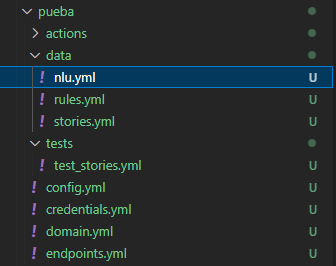
\includegraphics[width=0.8\textwidth]{imagenes/0008a-estructuraRasa.png}
					\caption{Estructura de Rasa}
                \end{subfigure}   
                \begin{subfigure}{0.45\textwidth}
                    \centering
					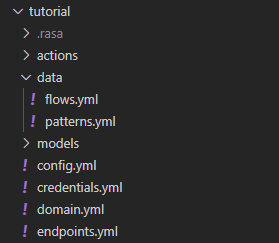
\includegraphics[width=0.8\textwidth]{imagenes/0008b-estructuraRasaPro.png}
					\caption{Estructura de Rasa Pro}
                \end{subfigure}                  
				\caption{Comparación de las dos estructuras}
				\label{fig:0008-comparacionEstructuras}
            \end{figure}

            \noindent Estos nuevos archivos engloban los flujos de conversación (ver figura \ref{fig:0009-ficheroNuevos}) que el asistente debe seguir. Los flujos están diseñados para recoger toda la información necesaria para realizar el proceso que tienen programado.

            \begin{figure}[H]
                \centering
                \begin{subfigure}{0.49\textwidth}
                    \centering
					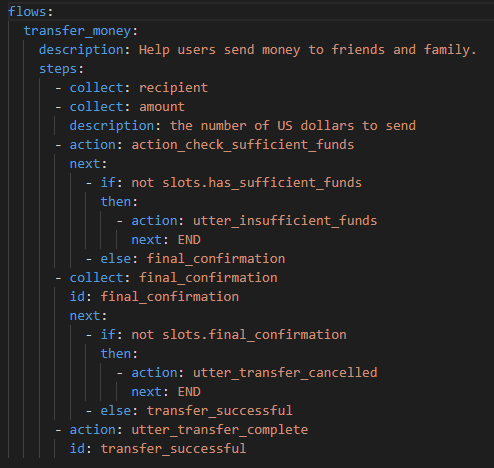
\includegraphics[width=0.9\textwidth]{imagenes/0009a-flows.png}
					\caption{flows.yml}
                \end{subfigure}   
                \begin{subfigure}{0.45\textwidth}
                    \centering
					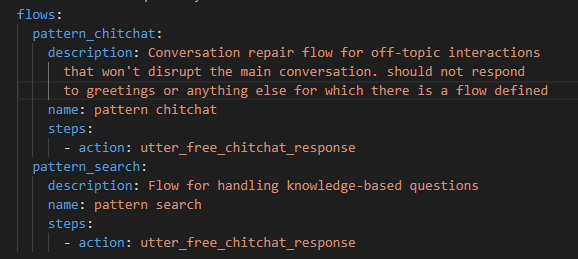
\includegraphics[width=0.9\textwidth]{imagenes/0009b-patterns.png}
					\caption{patterns.yml}
                \end{subfigure}                  
				\caption{Contenido de los ficheros flows.yml y patterns.yml}
				\label{fig:0009-ficheroNuevos}
            \end{figure}

            \noindent Los llamados \textit{Slots} (la memoria del asistente) son leídos en el flujo mediante la etiqueta \textit{collect} y son manejados, al igual que las respuestas, de la misma manera que con Rasa Open Source, en el archivo \textit{domain.yml}. Es posible añadir un prompt en este archivo para ayudar al modelo a manejar las respuestas (ver figura \ref{fig:0010-respuestaPrompt})

            \begin{figure}[H]
                \centering
                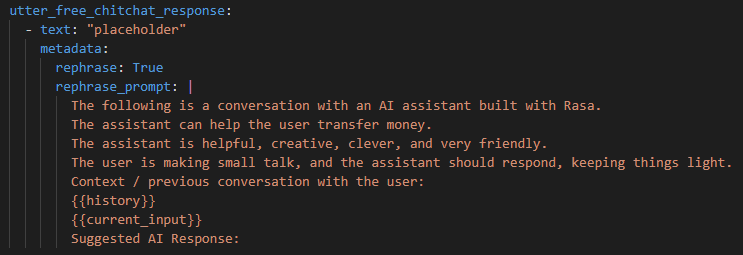
\includegraphics[width=0.9\textwidth]{imagenes/0010-respuestaPrompt.png}
                \caption{Ejemplo de una respuesta con prompt integrado}
                \label{fig:0010-respuestaPrompt}
            \end{figure}

            \noindent En resumen, los cambios que aporta esta versión hacen que controlar el flujo de conversación sea más sencillo y claro. Ahora las intenciones de usuario, son deducidas gracias al uso de modelos de lenguaje. El código es fácil de adaptar a las necesidades de cualquier proyecto y permite controlar las respuestas dadas por el asistente, debido a que todo este permanece \textit{on premise}.

        \subsection{Rendimiento}

            El asistente de prueba de Rasa Pro usa por defecto un modelo de lenguaje desarrollado por la misma empresa: \textbf{codellama} \cite{0009_CodeLlama}. Este modelo ya esta preparado para usarse en asistentes implementados bajo el CALM, es decir, este modelo traduce los mensajes enviados por un usuario a los comandos que son necesarios para avanzar en la conversación. De acuerdo a la documentación, este modelo no es capaz de generar texto arbitrario o creativas, ni texto problemático o dañino.

            \noindent A la hora de probar el modelo, Rasa Pro incluye un modo ``inspector", nos permite visualizar en una interfaz de navegador un grafo con el flujo de conversación en tiempo real (ver figura \ref{fig:0011-grafoFlujo}).      

            \begin{figure}[H]
                \centering
                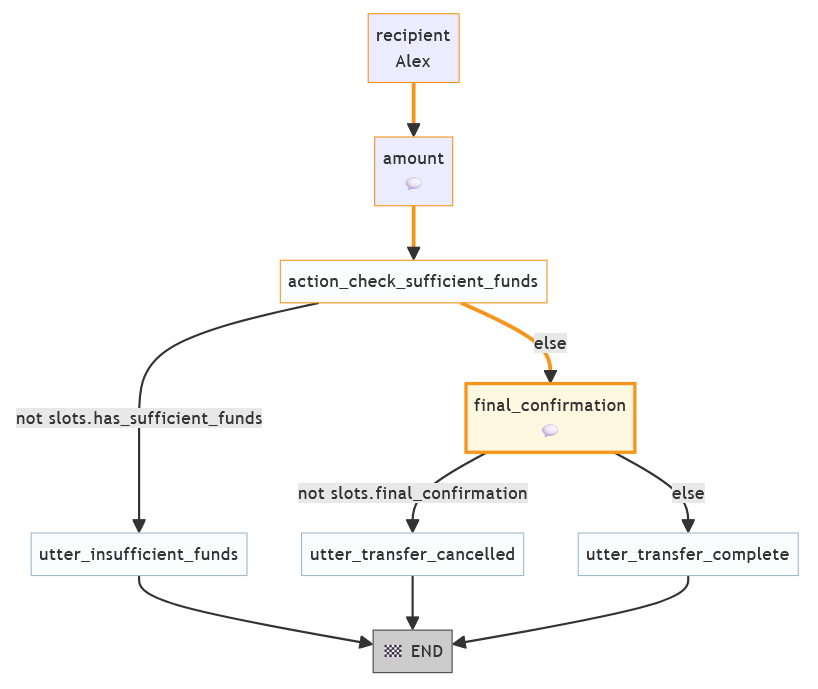
\includegraphics[width=.8\textwidth]{imagenes/0011-grafoFlujo.png}
                \caption{El inspector nos muestra un grafo con el flujo de conversación}
                \label{fig:0011-grafoFlujo}
            \end{figure}

            \noindent Otro aspecto importante es, que en las conversaciones podemos optar por dar los datos uno a uno o todos a la vez (ver figura \ref{fig:0012-convers}). Esta característica ya estaba presente en la versión anterior de Rasa (Rasa Open Source) y en esta la han mantenido.

            \begin{figure}[H]
                \centering
                \begin{subfigure}{0.49\textwidth}
                    \centering
					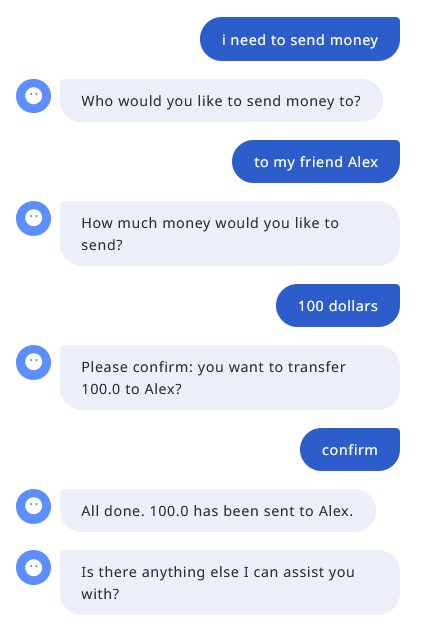
\includegraphics[width=0.9\textwidth]{imagenes/0012a-conversacion1.png}
					\caption{Datos uno a uno}
                \end{subfigure}   
                \begin{subfigure}{0.45\textwidth}
                    \centering
					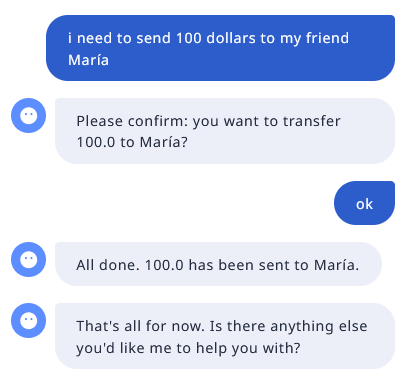
\includegraphics[width=0.9\textwidth]{imagenes/0012b-conversación.png}
					\caption{Todos los datos a la vez}
                \end{subfigure}                  
				\caption{Maneras en las que puedes conversar en una aplicación hecha con Rasa Pro}
				\label{fig:0012-convers}
            \end{figure}

            \noindent En cuanto al rendimiento, el tiempo de ejecución del modelo de prueba es casi inmediato. Sin embargo, como hemos mencionado anteriormente, la imposibilidad de este modelo a generar respuestas creativas, lo convierten en una opción no muy recomendable. 

            \noindent Rasa Pro permite modificar el modelo de lenguaje dentro de la configuración del proyecto, ofreciendo compatibilidad con modelos tanto locales como en la nube, incluyendo OpenAI y otras alternativas.

            \noindent En nuestras pruebas, utilizamos un modelo local \textit{llama3.2} descargado gracias a la plataforma \textbf{Ollama } (ver sección \ref{sec:ollama}). Los resultados obtenidos no fueron muy buenos, además de presentar tiempos de respuesta significativamente altos en comparación con el modelo anterior, en ocasiones omitía pasos dentro de la conversación. No se realizaron pruebas con modelos de OpenAI debido a la falta de clave de acceso a sus servicios.

            \subsection{Conclusión respecto a Rasa Pro}

                La integración de base de Rasa Pro con los modelos de lenguaje representa un avance significativo para el desarrollo de asistentes conversacionales en esta plataforma. Con la adopción del enfoque CALM \cite{0008_RasaCalm}, podemos gestionar diálogos de una forma más dinámica eliminando la necesidad de definir las intenciones explícitamente.

                \noindent Sin embargo y, como hemos mencionado en anteriores apartados, Rasa Pro cuenta con una serie de limitaciones que deben ser consideradas. Las restricciones puestas por su licencia gratuita pueden ser un obstáculo para aplicaciones que requieran una más alta cantidad de interacciones. El modelo de lenguaje de prueba incorporado, aunque ofrece respuestas en muy poco tiempo, su capacidad de generar respuestas es también limitada y puede no ajustarse a todos los casos de uso.

                \noindent En nuestras pruebas, el uso de modelos de lenguajes locales no logró resultados satisfactorios debido a unos tiempos de respuesta muy elevados y ciertas inconsistencias en la generación de respuestas.

                \noindent En definitiva, aunque Rasa Pro es una opción potente y viable para desarrollar asistentes conversacionales, presenta bastantes inconvenientes. Las limitaciones que tenemos tanto por la licencia como por el uso de modelos de lenguaje locales, nos hacen movernos hacia otras opciones de código libre (algunas ya mencionadas), que no requieren de licencia o que no ponen restricciones de uso.
    
    \section{Ollama}
    \label{sec:ollama}
        
        Ollama \cite{0010_Ollama1} es una herramienta de código abierto en la que podemos usar LLMs disponibles gratuitamente en nuestra propia máquina local (o servidor). Ollama actúa como un puente entre el modelo de lenguaje y nuestra máquina, no solo permitiéndonos usarlo, si no que también ofreciendo una API que podemos usar en aplicaciones más avanzadas.        

        \begin{figure}[H]
            \centering
            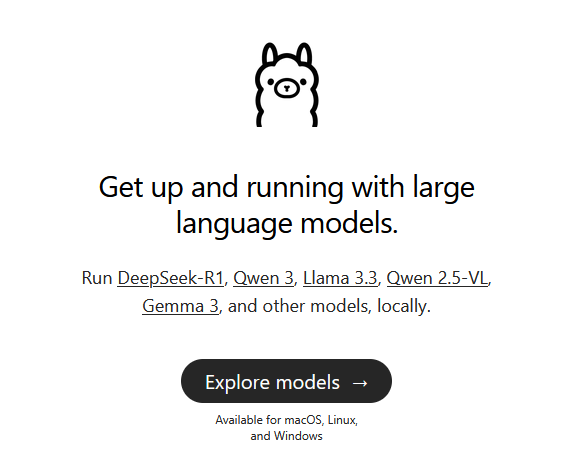
\includegraphics[width=.8\textwidth]{imagenes/0013_ollama.png}
            \caption{Sitio web oficial de Ollama: \url{https://ollama.com/}}
            \label{fig:0013_ollama}
        \end{figure}

        \noindent Al acceder localmente a los modelos, podemos mantener un control total sobre los datos y, evitar la inseguridad o los riesgos asociados con los servicios en la nube. Además, las herramientas sin conexión que ofrece Ollama ayudan a reducir latencias y dependencias de servidores externos, haciéndolas más rápidas (dependiendo mucho del equipo en el se ejecute) y confiables.

        \noindent En los siguientes apartados, repasaremos algunas de las características más importantes de esta herramienta y mostraremos un ejemplo de uso.
        
        \subsection{Características principales de Ollama}

            \subsubsection{Privacidad y acceso sin conexión}

                Es una de las principales características \cite{0010_Ollama1} que ofrece Ollama, la cual nos da la opción de ejecutar modelos de forma privada en nuestra máquina y sin conexión a Internet. De esta manera, podemos mantener nuestros datos de forma privada en nuestra equipo local sin que sean enviados a través de la red. Esta es una gran ventaja de Ollama sobre otros servicios en la nube, que podrían usar nuestros datos para otros propósitos.

            \subsubsection{Manejo de modelos}

                Añadir modelos a nuestra librería \cite{0010_Ollama1} local de Ollama es un proceso muy sencillo (tal y como se describe en la sección \ref{sec:ints&func_Ollama}). En el momento de escribir esta memoria el repositorio de Ollama cuenta con más de 150 modelos listos para usarse, desde \textit{Deepseek R1} hasta otros más populares como \textit{Llama3}, \textit{Gemma3}, \textit{Qwen2.5} o \textit{Mistral}. La web oficial de Ollama cuenta con la lista de los modelos disponibles.

            \subsubsection{Integración sencilla}

                Ollama se puede integrar fácilmente con una amplia variedad de herramientas, librerías y lenguajes de programación, por lo que es sencillo para los programadores incorporar LLMs en su flujo de trabajo \cite{0010_Ollama1,0011_Ollama2}. A parte de \textit{Python}, \textit{LangChain} (ver sección \ref{sec:LangChain}) o \textit{LlamaIndex}, Ollama presenta unas opciones de integración efectivas para el desarrollo de aplicaciones y soluciones avanzadas basadas en la IA.

            \subsubsection{Personalización y ajuste (Fine-tuning)}

                Ollama también nos da la posibilidad de ajustar ciertos parámetros de los modelos, como por ejemplo el tamaño de la ventana de contexto que usa el modelo para generar su respuesta o la temperatura/creatividad al generar la misma. Además, Ollama incluye el mecanismo \textit{modelfile}, en el cual podemos editar los parámetros del modelo usando un modelo base (un ejemplo es mostrado en la figura \ref{fig:0014_ollama_modelfile}).

                \begin{figure}[H]
                    \centering
                    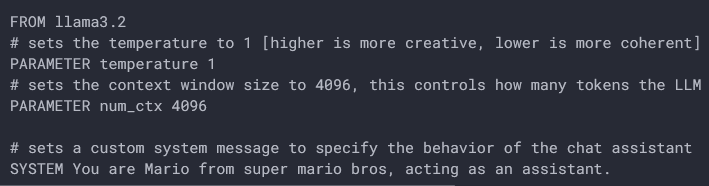
\includegraphics[width=.8\textwidth]{imagenes/0014_ollama_modelfile.png}
                    \caption{Fichero \textit{modelfile} básico, edita la temperatura y la ventana del contexto del modelo. Tiene de base el LLM \textit{Llama3.2}}
                    \label{fig:0014_ollama_modelfile}
                \end{figure}
                
        \subsection{Instalación y funcionamiento de Ollama}
        \label{sec:ints&func_Ollama}

            El archivo de instalación de Ollama se encuentra en su página web oficial, hay disponibles tres versiones para su descarga: \textit{Linux}, \textit{macOS} y \textit{Windows}. La instalación en \textit{Windows} no difiere de cualquier otro software para este sistema operativo, las otras dos versiones requieren de usar la consola para la instalación:

            \begin{itemize}            
                \item Para \textit{Linux}:
                    \begin{verbatim}
                        chmod +x ollama_linux.sh 
                        ./ollama_linux.sh
                    \end{verbatim}
                \item Para \textit{macOS}:
                    \begin{verbatim}
                        chmod +x ollama_macos.sh
                        ./ollama_macos.sh
                    \end{verbatim}
            \end{itemize}

            \noindent Una vez instalado, podemos usar Ollama mediante la consola de comandos de nuestro sistema. La siguiente figura muestra los comandos disponibles:

            \begin{figure}[H]
                \centering
                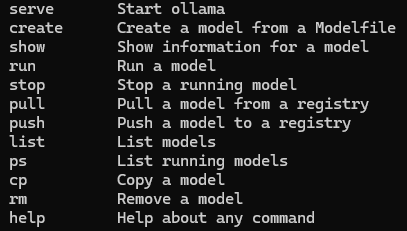
\includegraphics[width=.5\textwidth]{imagenes/0015_ollamaCMD.png}
                \caption{Lista de comandos disponibles de Ollama}
                \label{fig:0015_ollamaCMD}
            \end{figure}

            \noindent Como podemos observar en la figura \ref{fig:0015_ollamaCMD}, para usar un modelo tenemos dos opciones: la primera es descargarlo (\textit{pull}) y después ejecutarlo (\textit{run}), y la segunda es directamente ejecutarlo (\textit{run}), ya que lo descargará automáticamente. El comando \textit{serve} es también muy importante ya que inicia la API de Ollama.

            \noindent Por último, las figuras \ref{fig:0016_ollamaCLI} y \ref{fig:0017_ollamaPY}, muestran dos ejemplos de uso de los modelos: la primera figura muestra la ejecución desde línea de comandos, mientras que la segunda figura, muestra un pequeño programa escrito en \textit{Python} que además usa la librería \textit{LangChain} (sección \ref{sec:LangChain}).

            \begin{figure}[H]
                \centering
                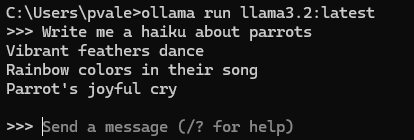
\includegraphics[width=.4\textwidth]{imagenes/0016_ollamaCLI.png}
                \caption{Prueba del CLI de Ollama, ejecuta el modelo \textit{Llama3.2} para hacer una consulta}
                \label{fig:0016_ollamaCLI}
            \end{figure}

            \begin{figure}[H]
                \centering
                \begin{subfigure}{0.49\textwidth}
                    \centering
					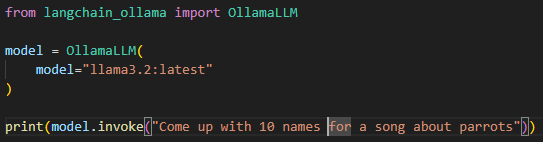
\includegraphics[width=0.9\textwidth]{imagenes/0017_ollamaPY1.png}
					\caption{Código de la aplicación}
                \end{subfigure}   
                \begin{subfigure}{0.49\textwidth}
                    \centering
					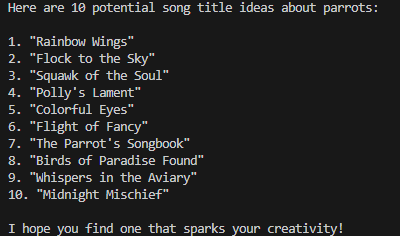
\includegraphics[width=0.9\textwidth]{imagenes/0017_ollamaPY2.png}
					\caption{Resultado de la ejecución}
                \end{subfigure}                  
				\caption{Pequeño programa escrito en \textit{Python}, usando la librería \textit{LangChain}. Pide al modelo \textit{Llama3.2} una consulta}
				\label{fig:0017_ollamaPY}
            \end{figure}
        
        \subsection{Alternativas: LM Studio}
        
            LM Studio \cite{0050_lmstudioDOCS} es aplicación multi-plataforma (\textit{Windows}, \textit{Linux} y \textit{macOS}) en la que podemos usar grandes modelos de lenguaje de forma local, sin conexión a la nube. Es similar a Ollama salvo que esta no es una opción de código abierto y además, cuenta con una interfaz gráfica sencilla e intuitiva (ver figura \ref{fig:0018_lmstudio}).

            \begin{figure}[H]
                \centering
                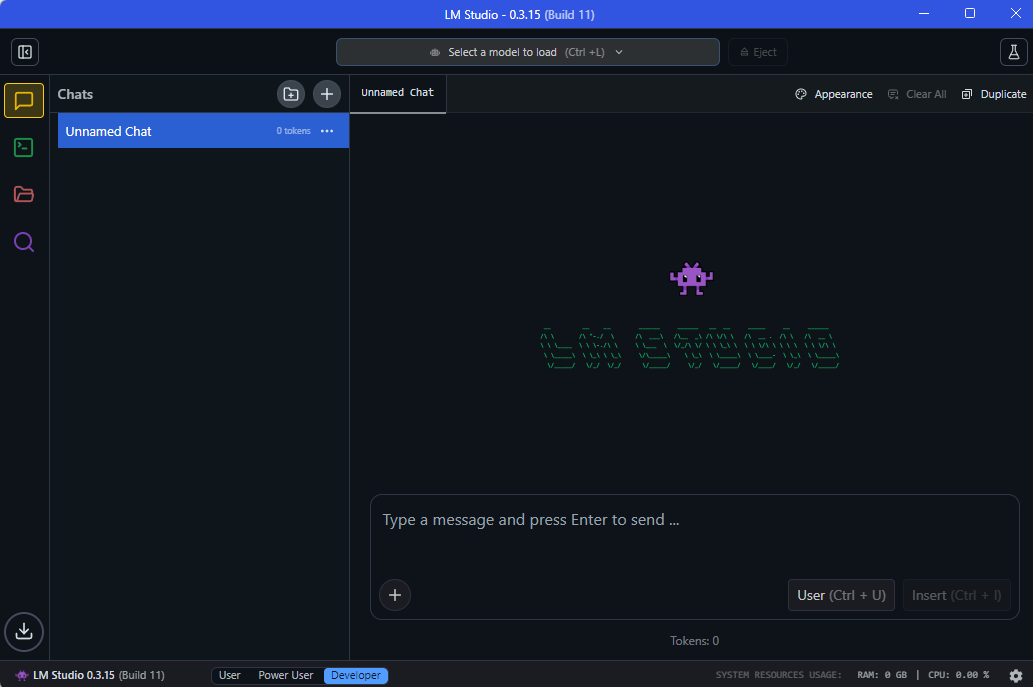
\includegraphics[width=.8\textwidth]{imagenes/0018_lmstudio.png}
                \caption{Pantalla principal de LM Studio, la pestaña activa nos permite chatear con un LLM}
                \label{fig:0018_lmstudio}
            \end{figure}

            \noindent Fijándonos en la figura \ref{fig:0018_lmstudio}, la parte de arriba posee una especie de botón usado para seleccionar y cargar el LLM que deseemos usar (ver figura \ref{fig:0019_lms_load}).

            \begin{figure}[H]
                \centering
                \begin{subfigure}{0.49\textwidth}
                    \centering
					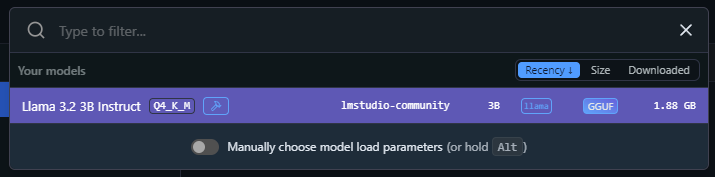
\includegraphics[width=0.9\textwidth]{imagenes/0019a_lms_llm.png}
					\caption{Selección}
                \end{subfigure}   
                \begin{subfigure}{0.49\textwidth}
                    \centering
					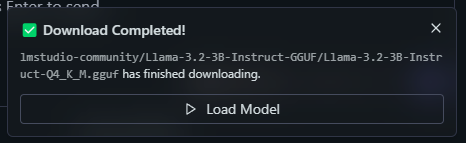
\includegraphics[width=0.9\textwidth]{imagenes/0019b_lms_load.png}
					\caption{Carga}
                \end{subfigure}                  
				\caption{Selección y carga de una versión de \textit{Llama3.2} en LM Studio}
				\label{fig:0019_lms_load}
            \end{figure}

            \noindent Siguiendo en la figura \ref{fig:0018_lmstudio}, la barra de la izquierda dispone de otras tres pestañas (de arriba a abajo):

            \begin{itemize}
                \item \textbf{Developer}: Nos permite activar o desactivar la API de LM Studio (ver figura \ref{fig:0020_lms_api}).
                \item \textbf{My models}: En la cual podemos ver los modelos descargados (figura \ref{fig:0021_lms_models}).
                \item \textbf{Discover}: Permite descargar nuevos modelos (figura \ref{fig:0022_lms_discoverpng}).
            \end{itemize}

            \begin{figure}[H]
                \centering
                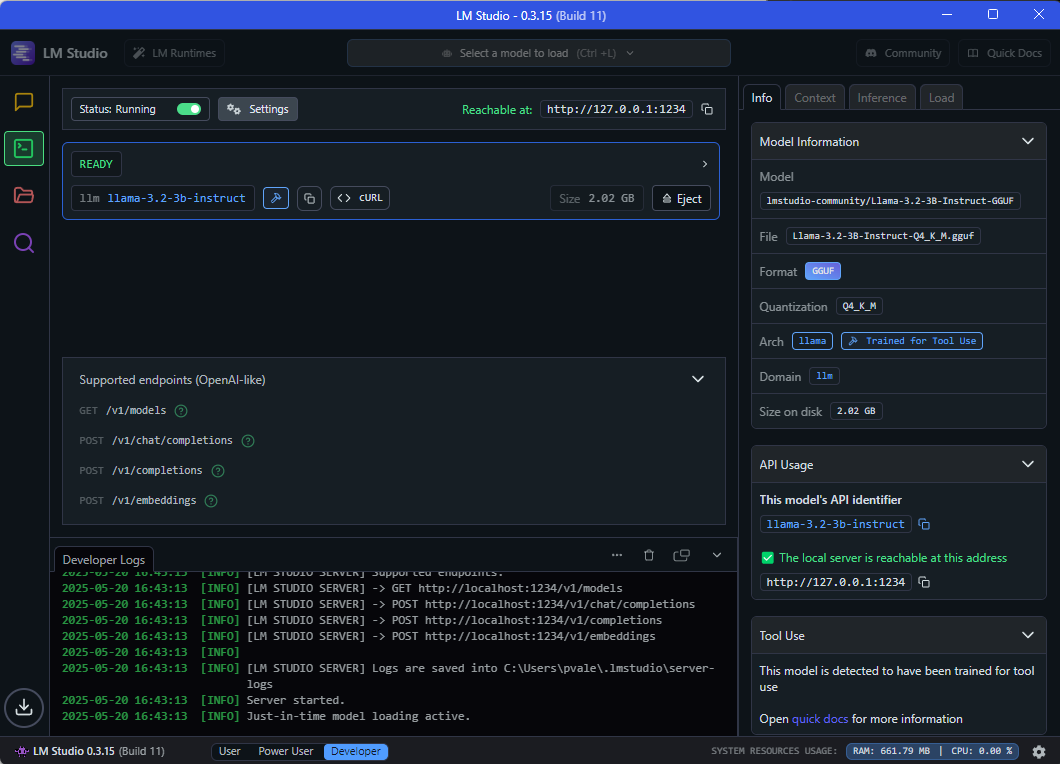
\includegraphics[width=.8\textwidth]{imagenes/0020_lms_api.png}
                \caption{Developer. Pestaña que permite controlar la API de LM Studio, se observa el modelo cargado, la dirección IP de esta y los logs}
                \label{fig:0020_lms_api}
            \end{figure}

            \begin{figure}[H]
                \centering
                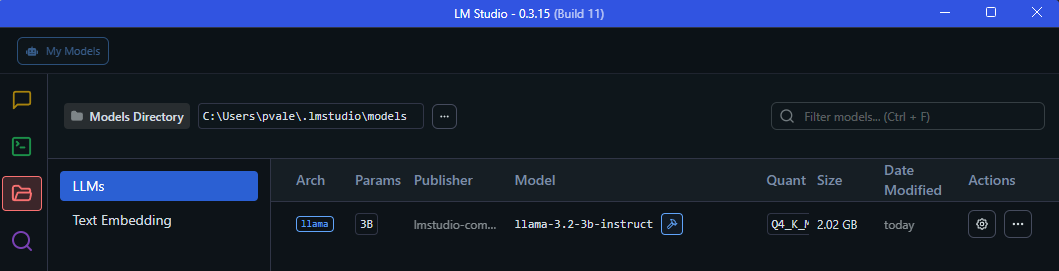
\includegraphics[width=.8\textwidth]{imagenes/0021_lms_models.png}
                \caption{My Models. Pestaña que permite ver los LLMs descargados en LM Studio}
                \label{fig:0021_lms_models}
            \end{figure}

            \begin{figure}[H]
                \centering
                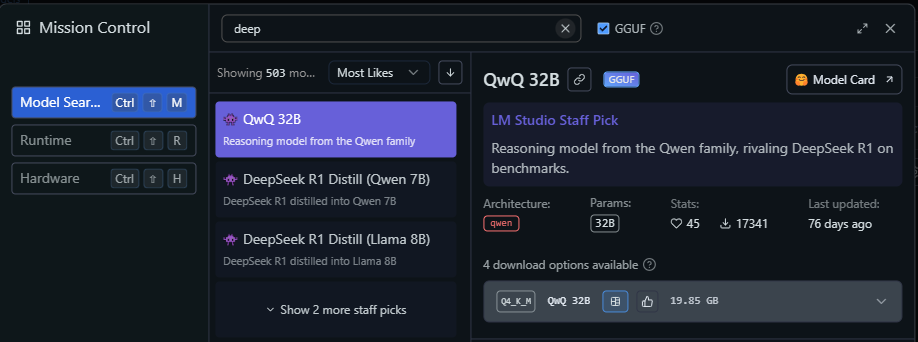
\includegraphics[width=.8\textwidth]{imagenes/0022_lms_discoverpng.png}
                \caption{Discover. Pestaña que permite descargar cualquier LLM disponible en LM Studio}
                \label{fig:0022_lms_discoverpng}
            \end{figure}            

            \subsubsection{Prueba de la API de LM Studio}

                Antes de poder probar la API de LM Studio, es necesario  instalar el paquete \textit{lmstudio} en nuestra instalación de \textit{Python}. Después con un código sencillo como el de la figura \ref{fig:0023_lms_python}, obtenemos una respuesta del LLM cargado previamente. 
                
                \noindent \textbf{Nota:}Aunque no se especifique en el código el LLM que debe usar, utiliza la versión de \textit{Llama3.2} cargada en la API que puede observarse en la figura \ref{fig:0020_lms_api}, en el lateral de de la derecha.
    
                \begin{figure}[H]
                    \centering
                    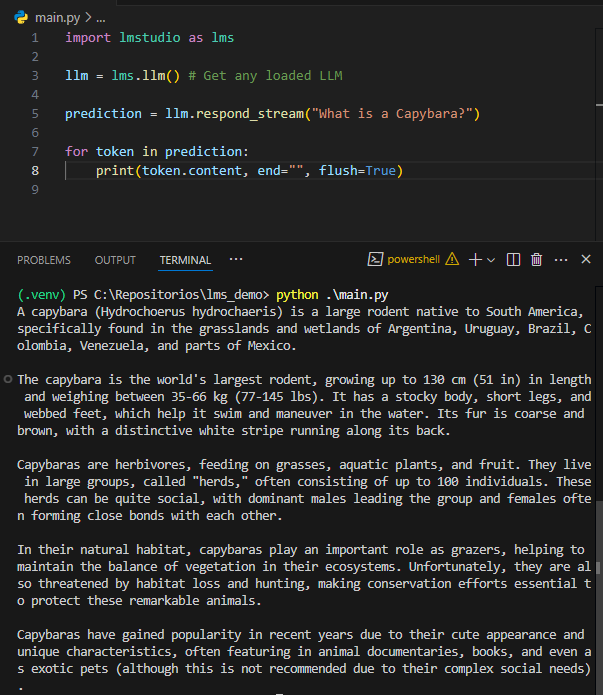
\includegraphics[width=.6\textwidth]{imagenes/0023_lms_python.png}
                    \caption{Pequeño código en Python, para la prueba de la API de LM Studio}
                    \label{fig:0023_lms_python}
                \end{figure}
            
            \subsubsection{Conclusiones: Ollama - LM Studio}

                Ollama y LM Studio presentan dos herramientas potentes para manejar LLMs de forma local. Aunque LM Studio ofrece una interfaz atractiva y sencilla de usar, son las integraciones de este las que dificultan su uso en aplicaciones más avanzadas. 
                
                \noindent Ollama esta pensado para esto último, siendo más sencillo de integrar con librerías externas, ya sean para ayudar en la recuperación de información (ChromaDB \ref{sec:chroma}) o dedicadas al manejo de LLMs (LangChain \ref{sec:LangChain}).

                \noindent Para finalizar, pese a que Ollama no cuenta con una interfaz gráfica, los comandos disponibles para la consola son intuitivos y fáciles de aprender, facilitando su adopción para usuarios menos expertos.

    \section{ChromaDB}
    \label{sec:chroma}

        ChromaDB \cite{0051_chromaDBDOCS} es una base de datos vectorial de código abierto, diseñada para almacenar y recuperar eficientemente vectores de embedding (sección \ref{sec:embeddings}), es decir, las representaciones numéricas de elementos como documentos de texto, imágenes, o vídeos. Su principal función es almacenar estas representaciones vectoriales con una serie de metadatos asociados para su posterior procesado por parte de un LLM. 

        \begin{figure}[H]
            \centering
            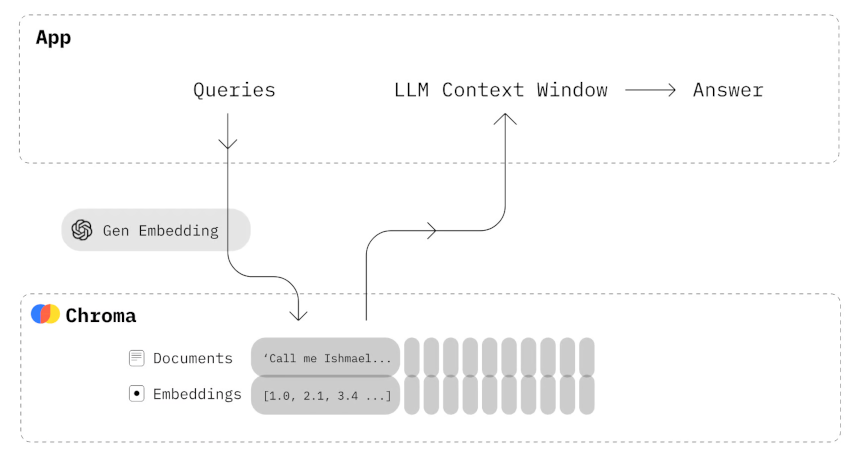
\includegraphics[width=.7\textwidth]{imagenes/0024_chroma.png}
            \caption{Esquema básico del funcionamiento de ChromaDB}
            \label{fig:0024_chroma}
        \end{figure}

        \subsection{Características de ChromaDB}

            ChromaDB posee un conjunto de características que hacen el adecuado para ser la base de datos vectorial de cualquier proyecto \cite{0013_chroma}. La lista siguiente muestra las más importantes:

            \begin{itemize}
                \item \textbf{Simple y potente:} Se instala con un simple comando ``\textit{pip install chromadb}'' y se integra sin problemas mediante la SDK de \textit{Python}, permitiendo una rápida configuración.
                \item \textbf{Multi-función:} Cuenta con una amplia gama de funcionalidades como la búsqueda vectorial, búsqueda de texto, almacenamiento de documentos, filtrado de metadatos, y recuperación multi-modal. Asimismo, es apto para aplicaciones que requieran una alta escalabilidad.
                \item \textbf{Gran soporte de lenguajes:} Ofrece SDKs para los lenguajes de programación más populares, incluyendo \textit{Python}, \textit{JavaScript/TypeScript}, \textit{Ruby}, \textit{PHP} y \textit{Java}.
                \item \textbf{Integración de base:} Cuenta con un enfoque de integración nativo para modelos de embedding de \textit{HuggingFace}, \textit{OpenAI}, \textit{Ollama}, y más. Del mismo modo, es compatible con las librerías \textit{LangChain}, \textit{LlamaIndex}, y muchas más previstas en un futuro.                
                \item \textbf{Almacenamiento local:} Las bases de datos pueden ser almacenadas tanto en memoria como en nuestro equipo local, manteniendo nuestra información privada y no dependiente de servicios externos.
                \item \textbf{Código abierto}: Bajo la licencia Apache2.0.
            \end{itemize}

        \subsection{Funcionamiento de ChromaDB}

            El funcionamiento de esta base de datos es simple y se puede poner en marcha rápidamente utilizando \textit{Python} \cite{014_chromaGS}. En la figura \ref{fig:0025_chromaGS} se muestra un método para crear la base de datos, añadir documentos y realizar consultas (líneas 4, 8 y 16 respectivamente).
    
            \begin{figure}[H]
                \centering
                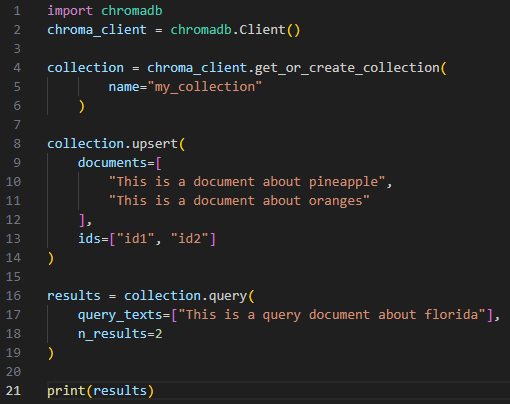
\includegraphics[width=.7\textwidth]{imagenes/0025_chromaGS.png}
                \caption{ChromaDB, puesta en marcha mediante \textit{Python}}
                \label{fig:0025_chromaGS}
            \end{figure}
            
            \noindent Existen varias formas de realizar cada uno de estos pasos. Por ejemplo, al crear el cliente Chroma, podemos especificar el modelo de embedding (por defecto se utiliza \textit{all-MiniLM-L6-v2}).
            
            \noindent En cuanto a la inserción de documentos, cuando la base de datos recibe un texto, lo convierte en su representación vectorial utilizando el modelo de embedding y asocia los metadatos correspondientes en el proceso.
            
            \noindent Finalmente, las consultas también se vectorizan utilizando el mismo modelo (preferiblemente y devuelven los documentos más relevantes mediante una función de búsqueda (por defecto, la similitud coseno).
            
            \noindent Los resultados (figura \ref{fig:0026_chromaGS2}) obtenidos al ejecutar el código mostrado en la figura anterior indican las distancias (línea 10) de los documentos recuperados. Estos resultados representan el output de la búsqueda en la base de datos, donde el documento cuyo ID es ``id2'' tiene una puntuación más alta (menos es mejor).
            
            \begin{figure}[H]
                \centering
                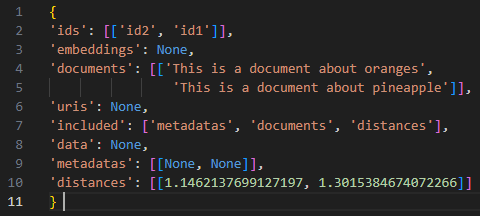
\includegraphics[width=.7\textwidth]{imagenes/0026_chromaGS2.png}
                \caption{ChromaDB. Resultados de la consulta, se observan las distancias de los documentos recuperados}
                \label{fig:0026_chromaGS2}
            \end{figure}            
        
        \subsection{Alternativas: Pinecone}            
            
            Pinecone \cite{0052_pineconeDOCS} es una base de datos vectorial gestionada en la nube \cite{0015_pinecone}, diseñada para realizar búsquedas en tiempo real por similaridad siendo altamente escalable. Esta tecnología ha ganado en popularidad por su facilidad de uso y por su rendimiento.

            \subsubsection{Pros y contras de Pinecone}

                Este modelo de recuperación contiene un conjunto de ventajas similar a ChromaDB con la única excepción del alojamiento web. Veamos algunas de ellas:

                \begin{itemize}
                    \item \textbf{Búsqueda en tiempo real}:  Pinecone ofrece una capacidad de búsqueda asombrosamente rápida, permitiendo a los usuario recuperar vectores similares en tiempo real. 
                    \item \textbf{Escalabilidad}: La arquitectura de Pinecone escala ante un crecimiento de la demanda.
                    \item \textbf{Indexado automático}: Los vectores son indexados automáticamente por Pinecone, reduciendo la carga de trabajo y simplificando el proceso de despliegue.
                    \item \textbf{Soporte Python}: La SDK de \textit{Python} es sencilla de utilizar, haciendo accesible Pinecone para todos los desarrolladores y científicos de datos familiarizados con este ecosistema.
                \end{itemize}

                \noindent Sin embargo, tiene dos inconveniente que podrían ser clave para un proyecto. Uno de ellos es el coste, al ser un servicio en la nube, Pinecone ofrece un modelos de negocio basado en tres tipos de categorías: \textit{Starter} gratuito y pensado para pequeñas aplicaciones, \textit{Standard} para aplicaciones de producción a cualquier escala y \textit{Enterprise} para aplicaciones críticas.

                \noindent La segunda desventaja es la funcionalidad limitada a la hora de realizar consultas avanzadas. A pesar de que Pinecone sobresale en búsquedas por similaridad, podría carecer de algunas capacidades de consulta avanzadas que ciertos proyectos requieren.

            \subsubsection{Funcionamiento de Pinecone}

                Para utilizar Pinecone antes debemos cumplir ciertos requisitos: tenemos que obtener una clave para su API y debemos instalar la SDK de \textit{Python}. La clave nos permite conectar con el servicio web, permitiéndonos crear índices (ver figuras \ref{fig:0028_pinecone1}, \ref{fig:0029_pinecone2} y \ref{fig:0029_pinecone21}) y enviar documentos (figuras \ref{fig:0030_pinecone3} y \ref{fig:0030_pinecone31}). 

                \begin{figure}[H]
                    \centering
                    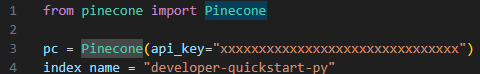
\includegraphics[width=.6\textwidth]{imagenes/0028_pinecone1.png}
                    \caption{Pinecone. Inicialización a través de su clave API}
                    \label{fig:0028_pinecone1}
                \end{figure} 

                \begin{figure}[H]
                    \centering
                    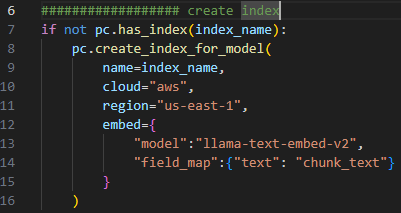
\includegraphics[width=.6\textwidth]{imagenes/0029_pinecone2.png}
                    \caption{Pinecone. Creación de un índice}
                    \label{fig:0029_pinecone2}
                \end{figure} 

                \begin{figure}[H]
                    \centering
                    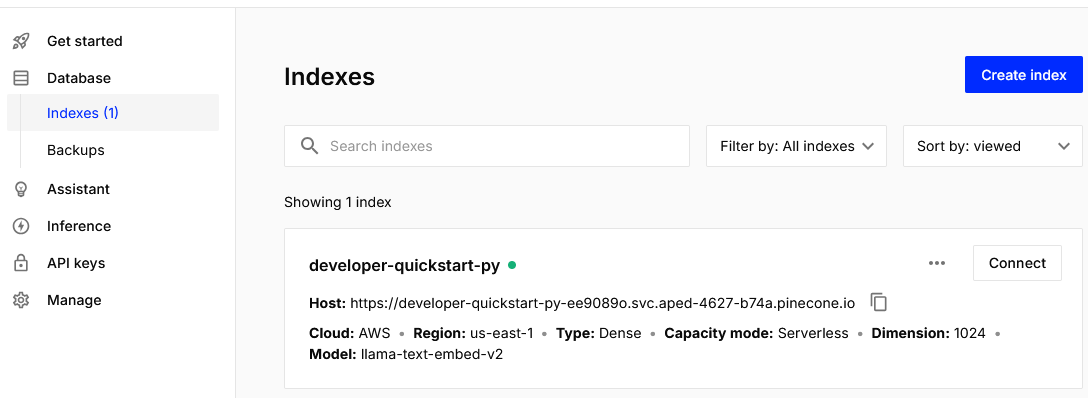
\includegraphics[width=.8\textwidth]{imagenes/0029_pinecone2-1.png}
                    \caption{Pinecone. Vista del índice en la web}
                    \label{fig:0029_pinecone21}
                \end{figure}     

                \begin{figure}[H]
                    \centering
                    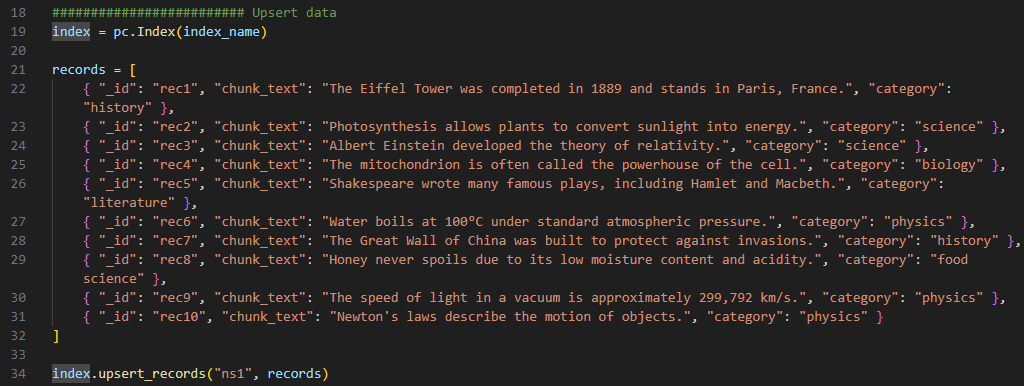
\includegraphics[width=.8\textwidth]{imagenes/0030_pinecone3.png}
                    \caption{Pinecone. Agregación de documentos}
                    \label{fig:0030_pinecone3}
                \end{figure} 

                \begin{figure}[H]
                    \centering
                    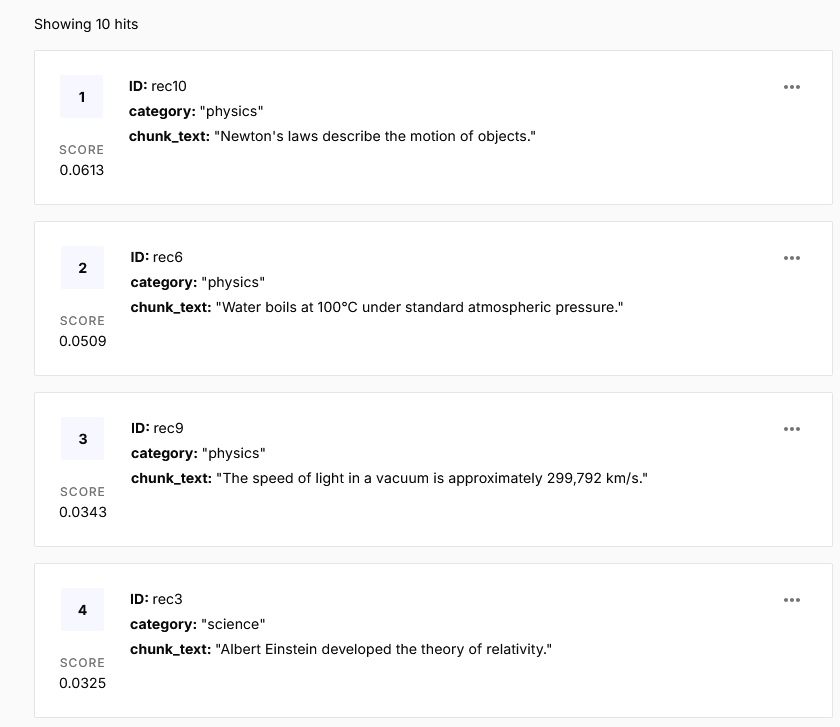
\includegraphics[width=1\textwidth]{imagenes/0030_pinecone3-1.png}
                    \caption{Pinecone. Vista de documentos en la web}
                    \label{fig:0030_pinecone31}
                \end{figure}        

                \noindent Las búsquedas en Pinecone se pueden realizar como se muestra en la siguiente figura: especificando la consulta y los parámetros de recuperación deseados (ver figura \ref{fig:0031_pinecone}). Pinecone ofrece también la posibilidad de hacer \textit{rerank} a los resultados (véase la figura \ref{fig:0032_pinecone}), es decir, un refinamiento o re-ordenación de los documentos recuperados basado en la relevancia ante una consulta.

                \begin{figure}[H]
                    \centering
                    \begin{subfigure}{0.49\textwidth}
                        \centering
    					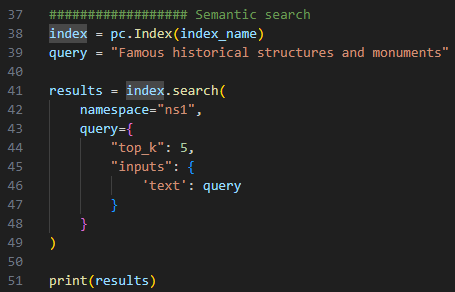
\includegraphics[width=0.9\textwidth]{imagenes/0031_pinecone4.png}
    					\caption{Búsqueda semántica}
                    \end{subfigure}   
                    \begin{subfigure}{0.49\textwidth}
                        \centering
    					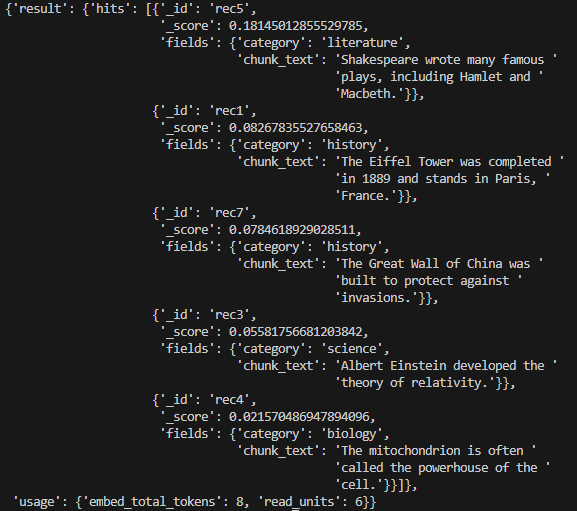
\includegraphics[width=0.9\textwidth]{imagenes/0031_pinecone5.png}
    					\caption{Resultados}
                    \end{subfigure}                  
    				\caption{Pinecone. Búsqueda semántica y resultados}
    				\label{fig:0031_pinecone}
                \end{figure}

                \begin{figure}[H]
                    \centering
                    \begin{subfigure}{0.49\textwidth}
                        \centering
    					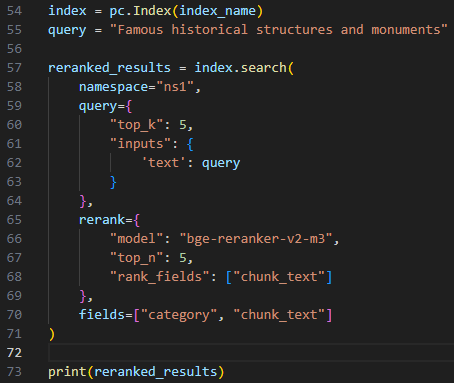
\includegraphics[width=0.9\textwidth]{imagenes/0032_pinecone6.png}
    					\caption{Reranking}
                    \end{subfigure}   
                    \begin{subfigure}{0.49\textwidth}
                        \centering
    					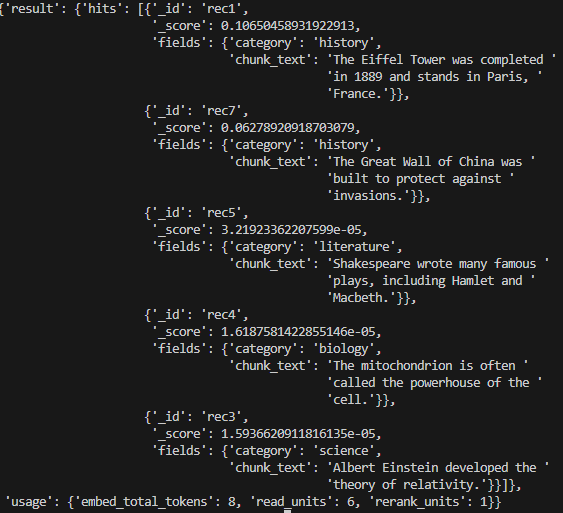
\includegraphics[width=0.9\textwidth]{imagenes/0032_pinecone7.png}
    					\caption{Resultados}
                    \end{subfigure}                  
    				\caption{Pinecone. Reranking y resultados}
    				\label{fig:0032_pinecone}
                \end{figure}

                \noindent Se puede observar una clara diferencia entre los resultados de las dos últimas figuras, siendo los obtenidos aplicando \textit{reranking} mucho más relevantes respecto a la consulta hecha.

            \subsubsection{Conclusión sobre Pinecone}
                
                Tras analizar el funcionamiento, características y diferencias entre ChromaDB y Pinecone, se puede concluir que ChromaDB representa una opción superior para muchos escenarios de desarrollo, especialmente aquellos en los que la privacidad, el control total sobre los datos y la independencia de servicios externos son prioritarios.

                \noindent La principal ventaja de ChromaDB reside en su capacidad para operar de manera local, sin necesidad de conexión a la nube. Esta característica permite que la información sensible se mantenga en el entorno del usuario, eliminando preocupaciones relacionadas con la exposición de datos o la dependencia de terceros. Además, su instalación sencilla, su compatibilidad con múltiples lenguajes y herramientas, y su naturaleza de código abierto lo convierten en una solución robusta y versátil para sistemas de recuperación de información basados en embeddings.
                
                \noindent Si bien Pinecone ofrece una infraestructura escalable y tiempos de respuesta rápidos, su condición de servicio en la nube introduce limitaciones importantes en términos de coste, privacidad y flexibilidad. Por tanto, para proyectos que requieran control local, transparencia y personalización, ChromaDB se posiciona como la alternativa preferente.

    \section{LangChain}
    \label{sec:LangChain}

        LangChain \cite{0053_langchainDOCS} se ha convertido en uno de los proyectos de código abierto con más rápido crecimiento en la historia, debido en gran medida al creciente interés surgido en al ámbito de los LLMs \cite{0016_langchain}. LangChain es un framework centrado en el desarrollo de aplicaciones impulsadas por los grandes modelos de lenguaje, cubriendo cada etapa de la vida de la aplicación: desde el desarrollo usando componentes de código abierto de LangChain o integraciones de terceros, la producción con la herramienta inspectora \textit{LangSmith}, y el despliegue a través de \textit{LangGraph}.

        \noindent LangChain implementa una interfaz estandar para los LLMs y tecnologías relacionadas, como son los modelos de embedding y las bases de datos vectoriales, y esta integrado con cientos de proveedores.

        \begin{figure}[H]
            \centering
            \includegraphics[width=.6\textwidth]{imagenes/0033_LangChain1.jpg}
            \caption{Esquema que muestra las diferentes aplicaciones en las que podemos usar LangChain \cite{0017_langchain2}}
            \label{fig:0033_LangChain1}
        \end{figure} 

        \noindent La importancia de LangChain radica en un conjunto de factores. El primero de ellos es que simplifica el proceso de desarrollo, reduciendo la complejidad a la hora de construir aplicaciones LLM por medio de plantillas estructuradas. Esto permite a los desarrolladores hacer las aplicaciones de manera modular, haciendo que sean más fáciles de manejar y escalar.

        \noindent A parte, LangChain permite la integración con múltiples LLMs, permitiéndonos usar el que más nos apetezca. Por último, el sistema de ``\textit{chaining}'' (o encadenamiento) ofrece una forma eficiente de llamar a los modelos, lo que incrementa el rendimiento y la precisión de la aplicación \cite{0017_langchain2}.

        \subsection{Características e integraciones de LangChain}

            Aunque ya hemos comentado algunas de las características o integraciones de LangChain, a continuación comentaremos algunas de las más importantes que tiene.

            \subsubsection{Características}

                \begin{itemize}
                    \item \textbf{Diseño modular:} Divide el proceso de desarrollo en módulos manejables, cada uno, asumiendo un aspecto específico de la aplicación.
                    \item \textbf{Manejo del prompt:} Provee de herramientas para crear y manejar prompts de manera eficiente.
                    \item \textbf{Chaining:} Permite enlazar múltiples prompts y modelos para crear flujos de trabajo complejos.
                    \item \textbf{Manejo del output:} Facilita el post-procesado de la salida de los modelos proporcionando una mejor usabilidad.
                \end{itemize}

            \subsubsection{Integraciones}    

                \begin{itemize}
                    \item \textbf{OpenAI GPT:} Una de las librerías de LLMs más usadas para el procesado del lenguaje natural.
                    \item \textbf{Mistral AI:} Un LLM desarrollado por la empresa del mismo nombre, diseñada para proporcionar información precisa y asistencia en una variedad de temas.
                    \item \textbf{Ollama:} Una biblioteca donde podemos encontrar una gran cantidad de LLMs de libre acceso.
                    \item \textbf{Hugging Face Transformers:} Una librería que da acceso a un gran número de modelos pre-entrenados.
                    \item \textbf{ChromaDB:} La base de datos vectorial usada en el proyecto.
                \end{itemize}

            \subsection{Tutorial básico de LangChain}

                Las siguientes figuras muestran una pequeña aplicación hecha usando LangChain y el resultado de su ejecución. En la figura \ref{fig:0034_langchain2} podemos ver el diseño modular y las integraciones antes mencionadas que tiene esta herramienta. Podemos observar también el diseño sencillo y sin complicaciones que ofrece a la hora de manejar prompts e integraciones con LLMs.

                \begin{figure}[H]
                    \centering
                    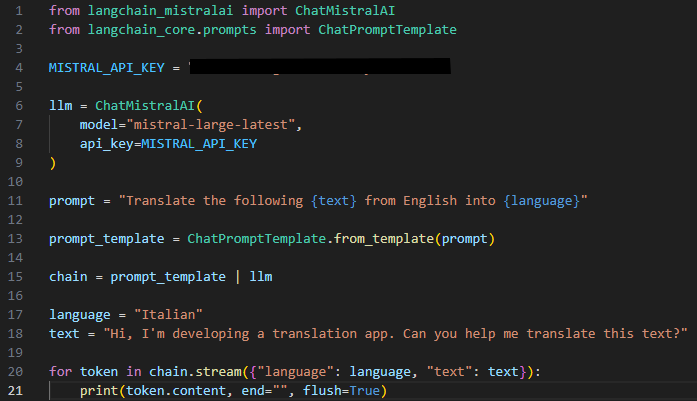
\includegraphics[width=.8\textwidth]{imagenes/0034_langchain2.png}
                    \caption{LangChain. Aplicación sencilla que usa mistral-large (LLM desarrollado por MistralAI) para traducir un texto}
                    \label{fig:0034_langchain2}
                \end{figure}    

                \begin{figure}[H]
                    \centering
                    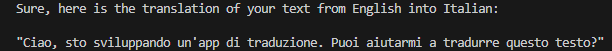
\includegraphics[width=.8\textwidth]{imagenes/0035_langchain3.png}
                    \caption{LangChain. Resultado de la traducción del texto de la figura \ref{fig:0034_langchain2}}
                    \label{fig:0035_langchain3}
                \end{figure}    
        
        \subsection{Alternativas: LlamaIndex}

            LlamaIndex \cite{0054_llamaindexDOCS} es la principal alternativa que tenemos a LangChain. LlamaIndex es un framework que simplifica la integración de datos públicos y privados en la construcción de aplicaciones usando grandes modelos de lenguaje \cite{0018_llamaindex}. Provee de funcionalidades para ingestar datos, indexación de datos, herramientas de búsqueda, etc, por lo tanto, es una solución muy versátil para construir un RAG.         

            \subsubsection{Funcionalidades principales y beneficios de LlamaIndex}

                El modo de operar de LlamaIndex se puede dividir en tres grandes bloques: ingestión, indexado y consulta \cite{0019_llamaindex2}.

                \noindent En la ingesta de datos, LlamaIndex simplifica el proceso de conectar con datos externos, desde APIs, PDFs o bases de datos. Esto asegura que datos con o sin estructura puedan ser integrados en aplicaciones LLM.

                \noindent Una vez los datos son ingestados, LlamaIndex dispone de múltiples modelos de indexación para representar datos de manera eficiente. Alguna de estas herramientas son:

                \begin{itemize}
                    \item \textbf{List Index}: Organizan los datos secuencialmente, apto para objetos estructurados que cambian en el tiempo.
                    \item \textbf{Tree Index}: Estructura los datos en forma de árbol.
                    \item \textbf{Vector Store Index}: Almacena los datos provenientes de un modelo de embedding, facilitando al vector hacer búsquedas por similaridad.
                    \item \textbf{keyword Index}: Asocia los metadatos a los datos almacenados.
                \end{itemize}

                \noindent Por último, a la hora de consultar, LlamaIndex aprovecha el procesado del lenguaje natural que posee para facilitar dichas consultas a través de un prompt. Este enfoque permite a los usuarios interactuar con los datos usando su propio lenguaje natural, simplificando el proceso de recuperación de información

            \subsubsection{Diferencias en el código: LangChain vs LlamaIndex}           
                A continuación mostraremos algunas figuras comparativas, donde veremos el código de LangChain y LlamaIndex para hacer una misma función.

                \begin{figure}[H]
                    \centering
                    \begin{subfigure}{0.49\textwidth}
                        \centering
    					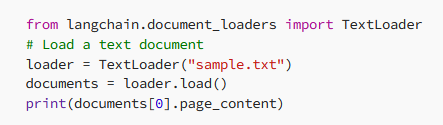
\includegraphics[width=1\textwidth]{imagenes/0037_loaders1.png}
    					\caption{LangChain}
                    \end{subfigure}   
                    \begin{subfigure}{0.49\textwidth}
                        \centering
    					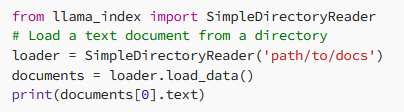
\includegraphics[width=1\textwidth]{imagenes/0037_loaders2.png}
    					\caption{LlamaIndex}
                    \end{subfigure}                  
    				\caption{Loaders, se encarga de cargar documentos \cite{0020_llamaindex3}}
    				\label{fig:0037_loaders}
                \end{figure}

                \begin{figure}[H]
                    \centering
                    \begin{subfigure}{0.49\textwidth}
                        \centering
    					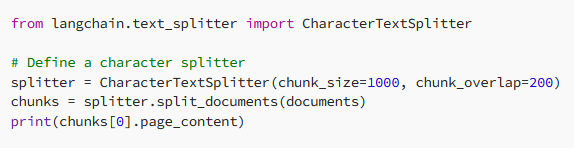
\includegraphics[width=1\textwidth]{imagenes/0038_splitters1.png}
    					\caption{LangChain}
                    \end{subfigure}   
                    \begin{subfigure}{0.49\textwidth}
                        \centering
    					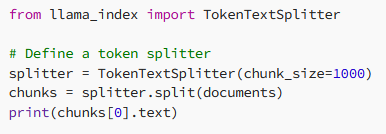
\includegraphics[width=1\textwidth]{imagenes/0038_splitters2.png}
    					\caption{LlamaIndex}
                    \end{subfigure}                  
    				\caption{Splitter, se encarga de trocear los documentos \cite{0020_llamaindex3}}
    				\label{fig:0038_splitters}
                \end{figure}

                \noindent Podemos apreciar en las figuras \ref{fig:0037_loaders} y \ref{fig:0038_splitters}, que la forma que tienen ambas herramientas de cargar y separar documentos es similar, usando sendas funciones con las que obtienen el mismo resultado.

                \begin{figure}[H]
                    \centering
                    \begin{subfigure}{0.49\textwidth}
                        \centering
    					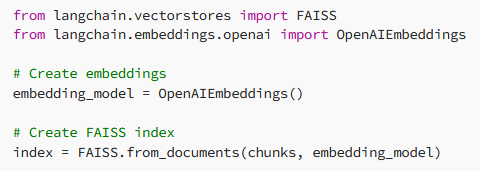
\includegraphics[width=1\textwidth]{imagenes/0039_indexing1.png}
    					\caption{LangChain}
                    \end{subfigure}   
                    \begin{subfigure}{0.49\textwidth}
                        \centering
    					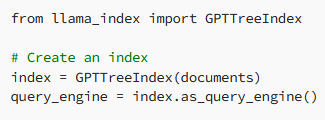
\includegraphics[width=1\textwidth]{imagenes/0039_indexing2.png}
    					\caption{LlamaIndex}
                    \end{subfigure}                  
    				\caption{Indexing, se encarga de almacenar los documentos en la base de datos vectorial \cite{0020_llamaindex3}}
    				\label{fig:0039_indexing}
                \end{figure}

                \noindent En cambio, la figura anterior muestra una diferencia. Por un lado, LangChain muestra su capacidad de integración personalizando los modelos de embedding y la base de datos a usar, mientras que LlamaIndex simplifica este proceso creando una estructura jerárquica y usando valores por defecto.

                \begin{figure}[H]
                    \centering
                    \begin{subfigure}{0.49\textwidth}
                        \centering
    					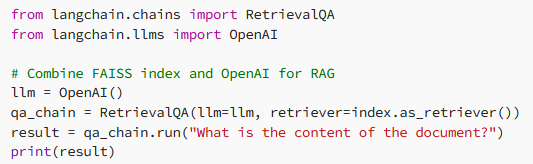
\includegraphics[width=1\textwidth]{imagenes/0040_chains1.png}
    					\caption{LangChain}
                    \end{subfigure}   
                    \begin{subfigure}{0.49\textwidth}
                        \centering
    					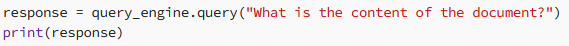
\includegraphics[width=1\textwidth]{imagenes/0040_chains2.png}
    					\caption{LlamaIndex}
                    \end{subfigure}                  
    				\caption{Chains/Query, se encarga de hacer una consulta a la base de datos vectorial \cite{0020_llamaindex3}}
    				\label{fig:0040_chains}
                \end{figure}

                \noindent A la hora de hacer consultas pasa algo similar a lo visto en la figura \ref{fig:0039_indexing}. La figura \ref{fig:0040_chains} muestra la forma de hacer una consulta con ambas herramientas, siendo mas simple la manera que ofrece LlamaIndex.               
            
            \subsubsection{Conclusión: LangChain vs LlamaIndex}

                Tras evaluar ambas herramientas, se ha determinado que LangChain es la opción más adecuada para el desarrollo de aplicaciones avanzadas basadas en LLMs. 
                
                \noindent LangChain destaca por su excepcional flexibilidad y capacidad de integración, permitiendo un control granular sobre cada componente del flujo de trabajo. Su capacidad para manejar flujos de trabajo multi-modales y su soporte para una amplia gama de modelos y bases de datos vectoriales lo posiciona como una herramienta poderosa para aplicaciones que demandan un alto nivel de personalización. Además, ofrece una interfaz estandarizada, que facilita la integración con multitud de proveedores y simplifica el proceso de desarrollo.
                
                \noindent Aunque LlamaIndex ofrece una solución más sencilla y directa, especialmente adecuada para proyectos que se centran en la recuperación y el procesamiento de documentos estructurados de manera jerárquica, su enfoque simplificado y facilidad de configuración no son suficientes para proyectos que requieren un alto nivel de personalización y control. LangChain, por otro lado, proporciona una infraestructura robusta y versátil que puede adaptarse a una amplia variedad de necesidades y complejidades del proyecto.
                
                \noindent Por lo tanto, LangChain se presenta como la opción superior para aquellos que buscan una solución altamente personalizable y con capacidad de manejar múltiples tipos de datos y estrategias de recuperación complejas. Su capacidad para integrarse con una amplia variedad de modelos y sistemas de almacenamiento, junto con su diseño modular y herramientas avanzadas para el manejo de prompts y outputs, lo convierten en la elección ideal para el desarrollo de aplicaciones avanzadas basadas en LLMs.
            
    \section{Streamlit}
    \label{sec:2_streamlit}

        Streamlit \cite{0055_streamlitDOCS} es un framework de código abierto en Python pensado para desarrollar aplicaciones interactivas basadas en el aprendizaje automático, inteligencia artificial o ciencia de datos. Streamlit permite a los desarrolladores y científicos de datos crear aplicaciones atractivas, informativas o realizar visualizaciones de datos en pocas líneas de código.

        \noindent Una de las principales aspectos de Streamlit es su simpleza y facilidad de aprendizaje. Además, Streamlit dispone de una amplia gama de herramientas o \textit{widgets} de visualización de datos: gráficas, histogramas, mapas, etc \cite{0022_streamlit2}.

        \noindent Otra ventaja de Streamlit es su flexibilidad, permitiendo desarrollar aplicaciones para un gran rango de casos de uso: desde simples código para visualizar datos, hasta aplicaciones complejas basadas en modelos de lenguaje.

        \subsection{Funcionalidades clave de Streamlit}

            Ya hemos mencionado algunos de sus aspectos más importantes, en la siguiente lista mostraremos los aspectos clave que hacen de Streamlit una de las herramientas más potentes \cite{0021_streamlit1}:

            \begin{itemize}
                \item \textbf{Desarrollo centrado en Python}: En contraste con los frameworks web tradicionales, esta herramienta usa Python. Elimina el requerimiento de usar lenguajes orientados a la web.
                \item \textbf{Widgets interactivos}: Como ya hemos comentado, Streamlit dispone de \textit{widgets} propios incluyendo botones, paneles desplegables, etc; que proporcionan más interactividad.
                \item \textbf{Actualizaciones en tiempo real}: Las aplicaciones Streamlit ejecutan el código de Python de arriba hacia abajo, actualizandose automáticamente cada vez que el usuario interactúa con un \textit{widget} o modifica una entrada de datos.
                \item \textbf{Soporte a la visualización de datos}: Streamlit esta integrado con las librerías de visualización de datos más comunes, incluyendo \textit{Seaborn} o \textit{Plotly}.
                \item \textbf{Prototipado rápido}: Streamlit posee una sintaxis sencilla, posibilitando un desarrollo de prototipos ágil y perfeccionamiento posterior.
                \item \textbf{De código abierto y extensible}: Al tener este enfoque, Streamlit confiere a los usuarios la posibilidad de extender su funcionalidad a través de plugins o integraciones hechos por la comunidad.
                \item \textbf{Opciones de despliegue}: Las aplicaciones desarrolladas en Streamlit pueden ser desplegadas en distintas plataformas como: Streamlit Community Cloud, Heroku, o AWS.
            \end{itemize}

        \subsection{Ejemplo de aplicación LLM en Streamlit}

            El siguiente ejemplo muestra una manera sencilla de integrar un LLM en Streamlit, usando varias librerías de LangChain, así como integraciones para los LLMs de Mistral AI y funcionalidades propias de Streamlit.

            \noindent En el caso de uso escogido para el ejemplo, simularemos una conversación con un agente IA que es un asistente de venta de vehículos. Para ello necesitaremos configurar un prompt donde recogeremos las instrucciones que deberá seguir el LLM en su respuesta. La siguiente figura muestra el prompt usado en la aplicación, y además, cuenta con dos variables, la consulta del usuario y el historial de la conversación. De esta manera podemos lograr que nuestro agente tenga memoria, lo que es muy útil en casos como este.
            
            \begin{figure}[H]
                \centering
                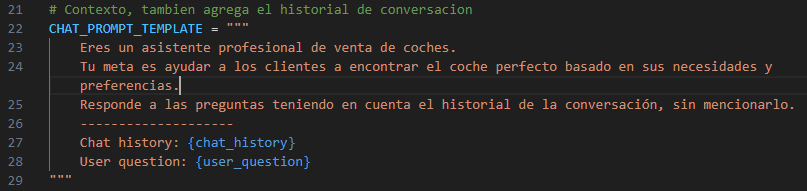
\includegraphics[width=.8\textwidth]{imagenes/0042_streamlit_ejemplo1.png}
                \caption{Ejemplo aplicación LLM en Streamlit. Prompt con dos varitables}
                \label{fig:0042_streamlit_ejemplo1}
            \end{figure}  

            \noindent Como hemos mencionado anteriormente, para este ejemplo hemos usado un LLM perteneciente a Mistral AI, en concreto, ``mistral-small'', dado a que es bastante rápido y eficiente. La figura \ref{fig:0043_streamlit_ejemplo2} muestra como se hace la llamada al LLM usando las herramientas que nos facilita LangChain, acabando retornando la ``chain'' o cadena en la que se escribirá la respuesta.
            
            \begin{figure}[H]
                \centering
                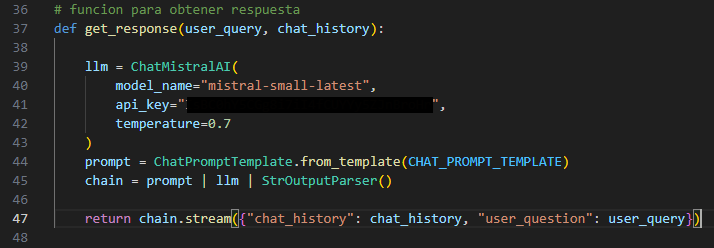
\includegraphics[width=.8\textwidth]{imagenes/0043_streamlit_ejemplo2.png}
                \caption{Ejemplo aplicación LLM en Streamlit. Llamada al LLM}
                \label{fig:0043_streamlit_ejemplo2}
            \end{figure}       

            \noindent El programa principal reflejado en la figura \ref{fig:0044_streamlit_ejemplo3}, no requiere de más de 20 líneas. Si nos fijamos en la línea 58, podemos observar como Streamlit gestiona las sesiones de estado para guardar el historial de conversación. Estas son variables especiales donde podemos guardar el valor de cualquier variable o clase.            

            \noindent La consulta de usuario se guarda fácilmente mediante el método \textit{chat\_input} de Streamlit, que crea en la interfaz un input para la entrada de texto. En las líneas 70 y 75 de figura \ref{fig:0044_streamlit_ejemplo3} podemos ver como se agregan la consulta y la respuesta del modelo a la variable que guarda el historial de conversación, mientras que en la 74, se hace una llamada a la función que retorna la respuesta del modelo. En concreto, el método \textit{write\_stream} de Streamlit escribe la respuesta en tiempo real según van llegando los \textit{tokens} del modelo de lenguaje, proporcionando una respuesta inmediata y una mejor experiencia de usuario.
            
            \begin{figure}[H]
                \centering
                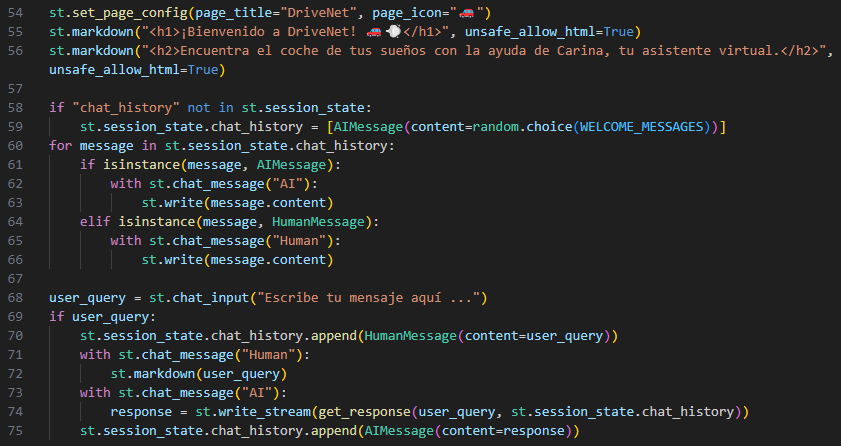
\includegraphics[width=1\textwidth]{imagenes/0044_streamlit_ejemplo3.png}
                \caption{Ejemplo aplicación LLM en Streamlit. Programa principal}
                \label{fig:0044_streamlit_ejemplo3}
            \end{figure}  

            \noindent En resumen, Streamlit se caracteriza por la sencillez de su código y por la integración que permite con otras herramientas como LangChain, etc. La siguiente subsección, muestra algunas capturas del funcionamiento de este ejemplo.

        \subsubsection{Funcionamiento del ejemplo}

            \begin{figure}[H]
                \centering
                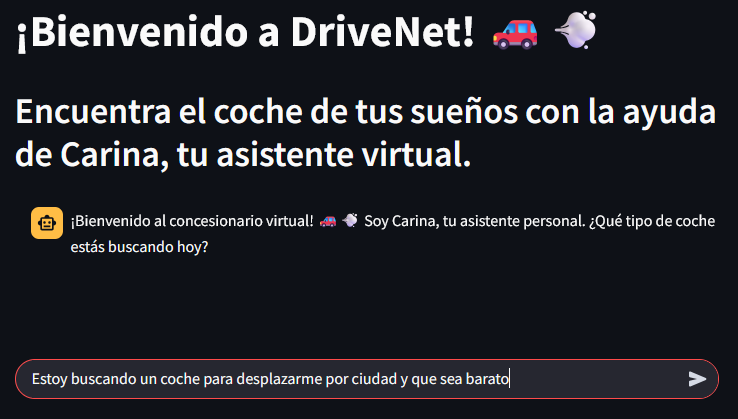
\includegraphics[width=.65\textwidth]{imagenes/0045_ejem1.png}
                \caption{Interfaz del ejemplo aplicación LLM en Streamlit. Bienvenida}
                \label{fig:0045_ejem1}
            \end{figure} 

            \begin{figure}[H]
                \centering
                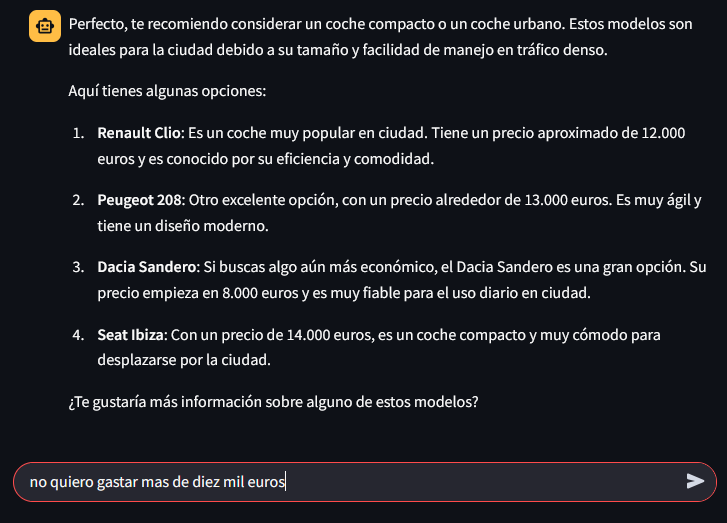
\includegraphics[width=.65\textwidth]{imagenes/0046_ejem2.png}
                \caption{Interfaz del ejemplo aplicación LLM en Streamlit. Opciones}
                \label{fig:0046_ejem2}
            \end{figure} 

            \begin{figure}[H]
                \centering
                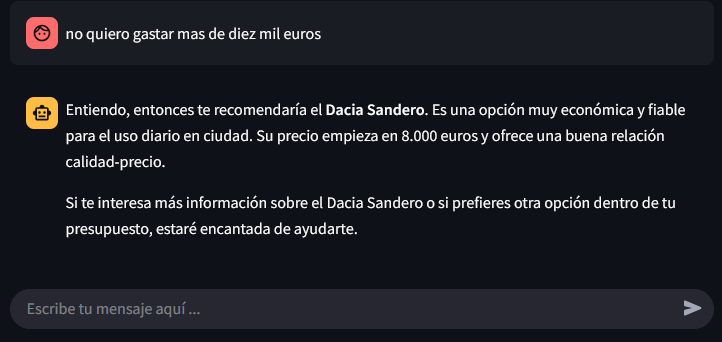
\includegraphics[width=.65\textwidth]{imagenes/0047_ejem3.png}
                \caption{Interfaz del ejemplo aplicación LLM en Streamlit. Respuesta con memoria}
                \label{fig:0047_ejem3}
            \end{figure} 
            
    \section{Aplicaciones alternativas al proyecto propuesto}
    
    	En esta sección hablaremos de aplicaciones o servicios similares a nuestro proyecto, aplicaciones de ayuda a ciudadanos ante una catástrofe natural, como la DANA; o servicios que usen de base un RAG para facilitar el acceso a la información. 
    	
    	\subsection{Ajuda Dana}
    	
    		Ajuda Dana \cite{0057_ajudana2} es una plataforma digital colaborativa creada tras la DANA en Valencia para coordinar de forma centralizada la ayuda a los afectados. Nació el 31 de octubre de 2024 a partir de la unión de iniciativas espontáneas en redes sociales, y que reunió a voluntarios de diferentes perfiles (informáticos, logísticos, atención al cliente, etc.), organizados como si fueran una empresa, pero sin apoyo oficial \cite{0057_ajudana}.
    		
    		\begin{figure}[H]
    			\centering
    			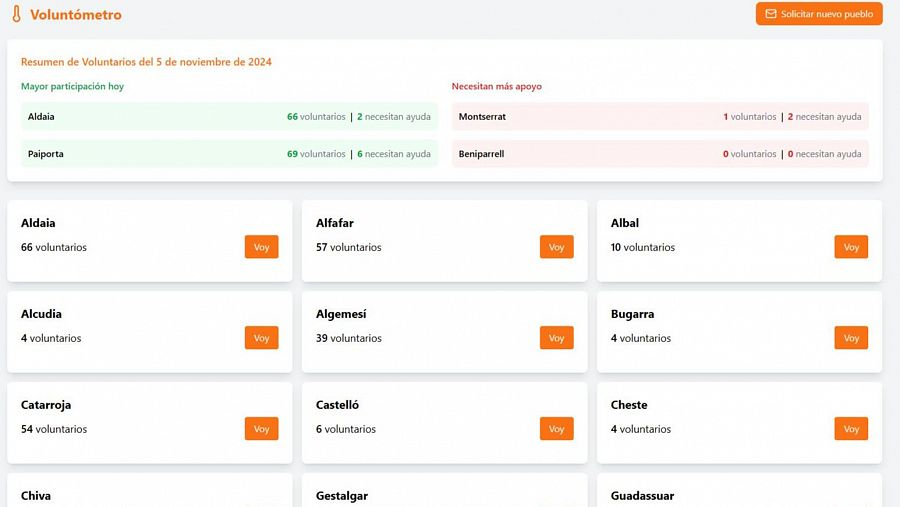
\includegraphics[width=.8\textwidth]{imagenes/0150_ajudana.jpg}
    			\caption{El voluntómetro muestra las solicitudes de ayuda y los voluntarios que hay en cada lugar \cite{0057_ajudana}}
    			\label{fig:0150_ajudana}
    		\end{figure} 
    		
    		\noindent La aplicación conecta solicitudes de ayuda con ofertas de voluntariado, gestionando peticiones y ofrecimientos en tareas como limpieza, alojamiento, asistencia médica, apoyo psicológico o transporte. Además, integra un servicio de búsqueda de desaparecidos, con el que han logrado localizar a 20 personas \cite{0057_ajudana}.
    		
    		\noindent Entre sus funcionalidades destacan:
    		
    		\begin{itemize}
    			\item Registro de solicitudes con niveles de urgencia (rojo, naranja, verde).
    			\item Mapa de puntos de recogida y distribución de suministros.
    			\item Teléfono gratuito para personas mayores sin acceso a internet.
    			\item Validación de información para evitar datos falsos.
    		\end{itemize}
    		
    		\noindent Ajuda Dana se ha convertido en una herramienta clave de coordinación ciudadana, combinando tecnología, voluntariado y solidaridad para dar respuesta rápida y eficaz a una emergencia colectiva.
    		
    	\subsection{TuCocheDana}
    	
    		TuCocheDANA era una plataforma digital creada durante la DANA para ayudar a propietarios a recuperar sus vehículos perdidos tras las riadas. La iniciativa fue desarrollada por Juan Francisco Soler, profesor de informática en el IES Alyanub de Almería, y su exalumno René Molina, estudiante de Ingeniería Mecánica en la UPV \cite{0058_tucochedana}.
    		
    		\noindent Su funcionamiento era sencillo:
    		
    		\begin{itemize}
    			\item Si una persona encontraba un coche abandonado, podía registrarlo indicando matrícula, ubicación, marca, color y detalles adicionales.
    			\item Si otra persona buscaba su coche perdido, bastaba introducir la matrícula en el buscador para obtener información y la localización exacta.
    		\end{itemize}   		
    		
    		\noindent La plataforma garantizaba la privacidad no proporcionando un listado abierto de coches encontrados, tan solo mostraba los datos vinculados a la matrícula introducida. Además, a través de un bot de Telegram, avisaba automáticamente a los propietarios cuando su coche fuese registrado, evitando así que tuviesen que comprobar la web de forma constante \cite{0058_tucochedana}.
    		
    		\noindent La plataforma funcionaba a través de la web tucochedana.es, que actualmente esta cerrada debido al tiempo transcurrido desde la tragedia.
    		
    		\noindent En resumen, TuCocheDANA fué un ejemplo de innovación digital solidaria, que combinó tecnología, colaboración ciudadana y gestión responsable de datos para resolver un problema muy concreto tras la catástrofe.
    		
    	\subsection{Justicio}
    	
	    	Justicio \cite{0060_justicio} es una plataforma de código abierto que utiliza un enfoque RAG, combinando la API de \textit{OpenAI} con la base de datos vectorial \textit{Qdrant}. Gracias a esta arquitectura, es capaz de entender consultas en lenguaje natural, recuperar información legislativa relevante y generar respuestas claras y fundamentadas, citando siempre las fuentes originales \cite{0060_justicio2}.
	    	
	    	\noindent Inicialmente concebido como un chatbot jurídico, Justicio se entrenó con legislación estatal, autonómica y europea, permitiendo a cualquier persona —desde juristas hasta ciudadanos sin formación legal— acceder de manera rápida y comprensible a normativas complejas. Su valor diferencial radica en transformar el BOE y otros textos legales densos y poco accesibles en respuestas útiles y contextualizadas \cite{0060_justicio3}.
	    	
	    	\noindent En 2025, la plataforma dio un paso más al lanzar un servicio gratuito que ofrece el acceso íntegro al BOE con una interfaz visual, estructurada y amigable (ver figura \ref{fig:0160_justicio}). Este nuevo sistema incluye:
	    	
	    	\begin{itemize}
	    		\item Un dashboard inicial con resúmenes y datos clave diarios.
	    		\item Secciones reorganizadas de manera comprensible y navegable.
	    		\item Herramientas para descargar, exportar y trabajar directamente con los documentos.
	    		\item Una doble modalidad de consumo: detallada o simplificada.
	    	\end{itemize}
	    	
	    	\begin{figure}[H]
	    		\centering
	    		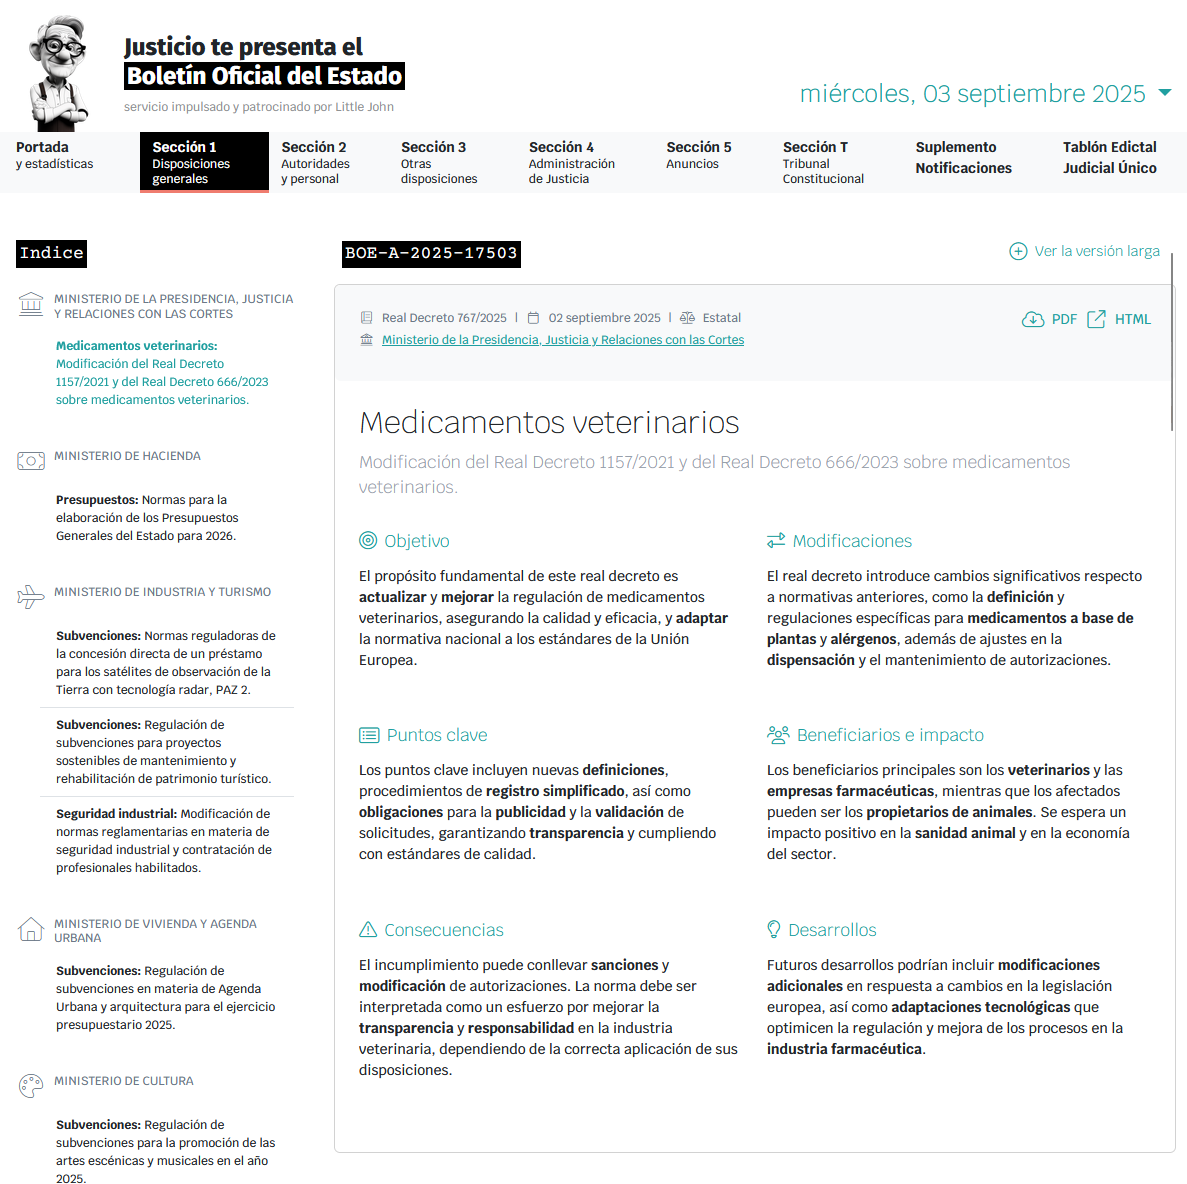
\includegraphics[width=1\textwidth]{imagenes/0160_justicio.png}
	    		\caption{Interfaz de Justicio en el BOE del día 3 de septiembre de 2025 \cite{0060_justicio}}
	    		\label{fig:0160_justicio}
	    	\end{figure} 
	    	
	    	\noindent Con esta evolución, Justicio no solo se ha consolidado como un ejemplo de aplicación práctica de RAG en el ámbito jurídico, sino que también ha logrado democratizar el acceso a la legislación española, transformando un recurso indispensable pero históricamente poco usable como el BOE en una herramienta realmente útil para profesionales y ciudadanos.
	    
	    \subsection{Conclusión sobre las aplicaciones alternativas}
	    
	    	En síntesis, proyectos como \textit{Ajuda Dana} y \textit{TuCocheDana} evidencian la capacidad de la tecnología para ofrecer soluciones útiles en situaciones de emergencia, mientras que \textit{Justicio} demuestra la aplicabilidad del enfoque RAG para hacer más accesible e interpretable la información contenida en el BOE. 
	    	
	    	\noindent En este contexto, el presente trabajo se sitúa en la misma línea, al proponer un sistema RAG aplicado a la documentación del BOE relativa a la DANA, con el fin de mejorar su comprensión y convertir un recurso jurídico denso en una herramienta práctica para la ciudadanía en momentos de crisis.
	    	
    \section{Métodos de evaluación de nuestro RAG}
    \label{2_metods_eva}

        En esta sección se describen las distintas técnicas y configuraciones que utilizaremos para evaluar nuestro sistema RAG. La evaluación se llevará a cabo mediante la combinación de diferentes procesos que afectan tanto a la recuperación de información como a la generación de respuestas. Para finalizar, evaluaremos diversas métricas con las que obtendremos el valor de calidad de los resultados.

        \noindent El conjunto de datos utilizado se almacena en forma de documentos en una base de datos vectorial \textbf{Chroma}, donde cada documento esta pre-procesado y segmentado en fragmentos de \textbf{512} y \textbf{1024} términos respectivamente. Esta decisión se ha tomado para evaluar la granularidad del contenido indexado y la relevancia de los documentos recuperados (enfoque \textit{Naive RAG}) \cite{gao2024retrievalaugmentedgenerationlargelanguage}, asi como la calidad del contexto aportado al modelo generativo.

        \noindent Paralelamente, se ha evaluado el impacto del \textbf{re-ranking} (enfoque \textit{Advanced RAG}) \cite{gao2024retrievalaugmentedgenerationlargelanguage} como paso posterior a la recuperación. Este proceso consiste en el reordenamiento de los documentos recuperados en primera instancia a través de un modelo de recuperación adicional. En nuestro caso usaremos el modelo \textbf{BAAI/bge-reranker-large} disponible en \textbf{HuggingFace} \cite{0036_bge_reranker}, que soporta documentos de más longitud, escritos en más idiomas (a parte del inglés) y a priori, logrará mejores resultados.

        \noindent En las siguiente sub-secciones, listaremos el resto de técnicas usadas para la evaluación del sistema RAG.

        \subsection{Estrategias de búsqueda usadas}

            Se han considerado varias estrategias de búsqueda a la hora de recuperar los documentos más relevantes de la base datos:
    
            \begin{itemize}
                \item \textbf{Similarity}: búsqueda por similitud mediante la distancia coseno en los embeddings.
                \item \textbf{Maximal Marginal Relevance (MMR)}: método usado para recuperar documentos que son a la vez relevante para consulta y diversos entre sí. Este enfoque ayuda a reducir la redundancia e incrementan las aspectos que son cubiertos en los documentos seleccionados \cite{0023_mmr}.
                \item \textbf{TF-IDF y BM25}: métodos clásicos basados en la frecuencia de los términos. TF-IDF se basa en la frecuencia y rareza de los términos del corpus, mientras que BM25 ajusta estos valores dependiendo del tamaño documento.
                \item \textbf{Grafo}: técnica que combina la búsqueda por similitud con relaciones semánticas obtenidas a través de los metadatos de los documentos \cite{peng2024graphretrievalaugmentedgenerationsurvey}. 
            \end{itemize}

        \subsection{Embeddings usados}

            Los embeddings utilizados para indexar y recuperar documentos incluyen los siguiente modelos pre-entrenados:

            \begin{itemize}
                \item \textbf{nomic-embed-text}: Modelo de código abierto entrenado en inglés. Es útil para clasificación, búsqueda y análisis semántico.
                \item \textbf{bge-m3}: Modelo multilingüe con más de cien idiomas. Optimizado para recuperación densa, escasa y multivectorial.
                \item \textbf{snowflake-artic-embed2}: Evolución del modelo anterior de Snowflake, con rendimiento similar a bge-m3. Es también multilingüe.
                \item \textbf{jina-embeddings-v2-base-es}: Biligüe español-inglés, ideal para realizar tareas en español: búsqueda, clasificación, etc.
                \item \textbf{text-embedding-3-small}: Versión mejorada del modelo anterior \textit{text-embedding-ada-002}, modelos pertenecientes a \textbf{OpenAI}.
            \end{itemize}

            \noindent Todos estos modelos están disponibles mediante la plataforma \textbf{Ollama}, exceptuando el último.

        \subsection{LLMs usados}

            Los modelos de lenguaje empleados son los siguientes.

            \begin{itemize}
                \item \textbf{llama3.2:} Modelo perteneciente a Meta de 3B de parámetros. Proporcionado localmente y de forma gratuita por Ollama.
                \item \textbf{mistral-small:} Versión 3.2 perteneciente a Mistral AI, cuenta con 24B de parámetros. Usado a través de la API gratuita de Mistral AI.
                \item \textbf{gpt-4.1:} Nuevo modelo perteneciente a OpenAI. De pago y disponible a través de clave API de OpenAI.
            \end{itemize}

        \subsection{Métricas de evaluación usadas}

            Para finalizar, presentaremos las métricas que se encargarán de medir la calidad de las respuestas de nuestro sistema RAG:

            \begin{itemize}
                \item \textbf{Accuracy}: Evalúa la precisión de la respuesta generada en comparación a la respuesta esperada.
                \item \textbf{Faithfulness}: Evalúa si la respuesta usa la información de los documentos recuperados.
                \item \textbf{Groundness}: Evalúa la capacidad del modelo de apoyar sus respuestas en las evidencias de los documentos recuperados.
                \item \textbf{Relevance}: Evalúa la relevancia de los documentos recuperados para responder a la pregunta.
            \end{itemize}

            \noindent Estas métricas evaluaran nuestro RAG a través de un dataset de preguntas generado a partir de los documentos de la fuente de conocimiento.

\begingroup
\titleformat{\chapter}[block]
{\normalfont\Huge\bfseries\centering} 
{Capítulo \thechapter} 
{0.5em}
{: \LARGE}
[\vspace{1em}\titlerule]

\titlespacing*{\chapter}{0pt}{-60pt}{40pt}

\chapter{Desarrollo del Proyecto}
\label{cap:3_dev}

    En este capítulo se describe el proceso de diseño, implementación y experimentación llevado a cabo para construir un sistema de generación aumentada por recuperación sobre un dominio específico, utilizando como fuente principal documentos del \textit{Boletín Oficial de Estado} (\textbf{BOE}) relacionados con la \textbf{DANA} ocurrida a finales del pasado año.

    \noindent La propuesta principal del proyecto es proveer de información veraz y actualizada a cualquier persona interesada en lo sucedido, por eso es fundamental la creación de un buen corpus que sirva como base para responder a nuestro sistema RAG.
    
    \noindent Por último, exploramos como distintas configuraciones del sistema, desde modelos de embeddings hasta las estrategias de búsqueda y generación (LLMs), afectan a la calidad y fiabilidad de las respuestas generadas. Los resultados provenientes de esta experimentación serán mostrados en el capítulo \ref{cap:4_results}.

    \section{Definición de la arquitectura}

        La arquitectura planteada para nuestro sistema RAG, es una combinación típica que se suele usar en la construcción de estos sistemas. Como se puede observar en la figura \ref{fig:0052_estructura}, el proceso para obtener una salida del RAG pasa por varias etapas.

        \begin{figure}[H]
            \centering
            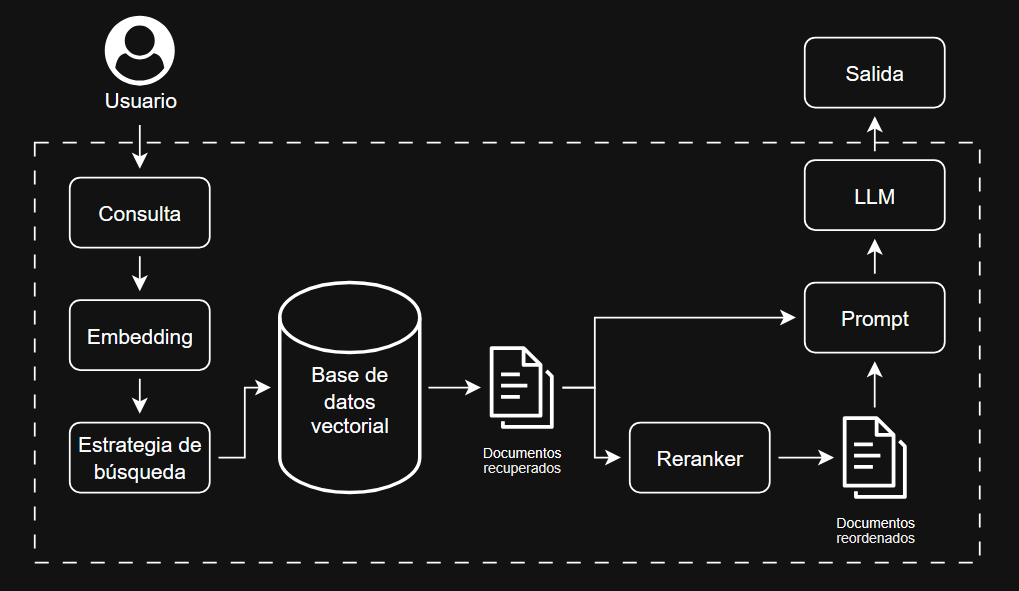
\includegraphics[width=0.8\textwidth]{imagenes/0052_estructura.png}
            \caption{Arquitectura de nuestro sistema RAG}		
            \label{fig:0052_estructura}
        \end{figure} 

        \noindent La consulta de usuario es vectorizada con el mismo modelo de embedding que hemos usado para la construcción de la base de datos vectorial para una mejor integridad de la respuesta, después es lanzada a la base de datos vectorial junto con la estrategia de búsqueda deseada.

        \noindent Los documentos recuperados son agregados al prompt para generar la respuesta usando el LLM que el usuario indique. Otra opción disponible en nuestro sistema, es la de usar un modelo de \textit{reranking} que filtre los documentos recuperados y seleccione los mejores para proporcionárselos de la misma manera al LLM mediante el prompt.

        \noindent La salida generada mostrará la información necesaria para responder a la entrada del usuario teniendo en cuenta el contenido relevante aportado por los documentos devueltos por el modelo de recuperación de información.

    \section{Planificación y presupuesto}
    
    	En esta sección explicaremos la planificación seguida en el proyecto, la metodología usada y todas las fases por las que pasamos durante el proceso de desarrollo de nuestra aplicación. Terminaremos la sección planteando el presupuesto estimado del proyecto, basándonos en los días transcurridos y en los integrantes pertenecientes al equipo de desarrollo.
    
    	\subsection{Metodología seguida: Scrum}

	        El proyecto se planifico desde un principio siguiendo el enfoque de las metodologías ágiles o \textbf{Scrum}. Este es un proceso en el que se aplican de manera regular un conjunto de buenas prácticas para trabajar colaborativamente, en equipo, y obtener el mejor resultado posible de un proyecto \cite{0028_scrum}. Aunque el ámbito de este Trabajo de Fin de Máster es individual, este proceso se sigue en la gran mayoría de empresas del sector de las tecnologías de la información, por lo que es interesante explorar su uso en el desarrollo de este proyecto.
	
	        \noindent Para llevar a cabo este seguimiento se propuso el uso de la herramienta \textit{Jira}, la cuál ofrece plantillas para crear la planificación de un proyecto siguiendo la metodología Scrum (figura \ref{fig:0053_jira-scrum}). Además, esta herramienta permite la conexión con repositorios de \textit{GitHub} (figura \ref{fig:0054_jira-github}) y asignar ramas de nuestro repositorio a las tareas contenidas en los tableros del sprint, de esta manera podemos mantener un cierto seguimiento en el avance del desarrollo en ambas plataformas.    
	
	        \begin{figure}[H]
	            \centering
	            
\includegraphics[width=0.7\textwidth]{imagenes/0053_jira-scrum.png}
	            \caption{Jira. Plantilla Scrum para el proyecto}		
	            \label{fig:0053_jira-scrum}
	        \end{figure} 
	
	        \begin{figure}[H]
	            \centering
	            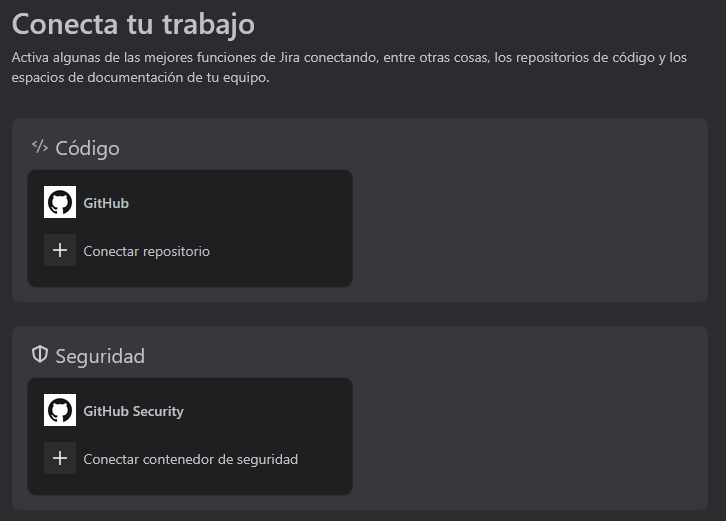
\includegraphics[width=0.6\textwidth]{imagenes/0054_jira-github.png}
	            \caption{Jira. Conexión con la plataforma de control de versiones GitHub}		
	            \label{fig:0054_jira-github}
	        \end{figure}         
	
	        \noindent En Scrum, un proyecto se ejecuta en ciclos temporales cortos y de duración fija llamados \textit{sprints}. En nuestro caso, estas iteraciones variaron entre 1, 2 o hasta 4 semanas dependiendo de la carga de trabajo o las tareas correspondientes al sprint. Cada sprint culminaba en una reunión presencial o vía telemática. donde se anunciaban los progresos alcanzados en el sprint, y se planeaban los objetivos para el siguiente.     
	
	        \noindent La figura \ref{fig:0056_jira-backlog} muestra la pestaña de \textit{Backlog}. Esta pestaña muestra en la parte superior todas las tareas que se tienen que cumplir en el sprint actual; y en la inferior, las tareas pendientes para futuros sprints. 
	
	        \begin{figure}[H]
	            \centering
	            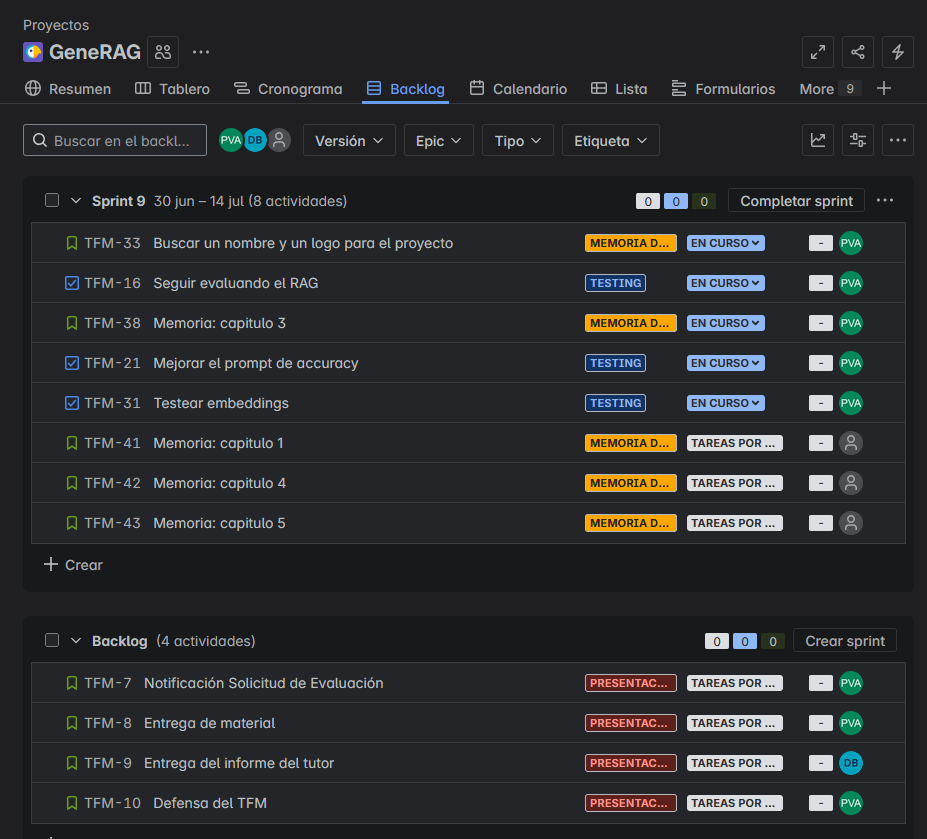
\includegraphics[width=0.7\textwidth]{imagenes/0056_jira-backlog.png}
	            \caption{Jira. Pestaña Backlog, tareas del sprint 9 y pendientes \cite{0056_proyectoJIRA}}		
	            \label{fig:0056_jira-backlog}
	        \end{figure} 
	
	        \noindent Una vez iniciado el sprint, en la pestaña \textit{Tablero} (figura \ref{fig:0058_jira-sprint2}) podemos ver las tareas asignadas anteriormente en el backlog y las columnas ``POR HACER", ``EN CURSO", ``EN REVISIÓN", y ``LISTO", columnas que podemos editar y añadir más. La lógica de estas columnas es mantener un control sobre que tarea se esta haciendo en este momento y quien es el encargado de ella. Cada tarea va avanzando hacia la columna de su derecha donde será evaluada hasta llegar a "LISTO", cuando podremos considerar la tarea acabada.        
	
	        \begin{figure}[H]
	            \centering
	            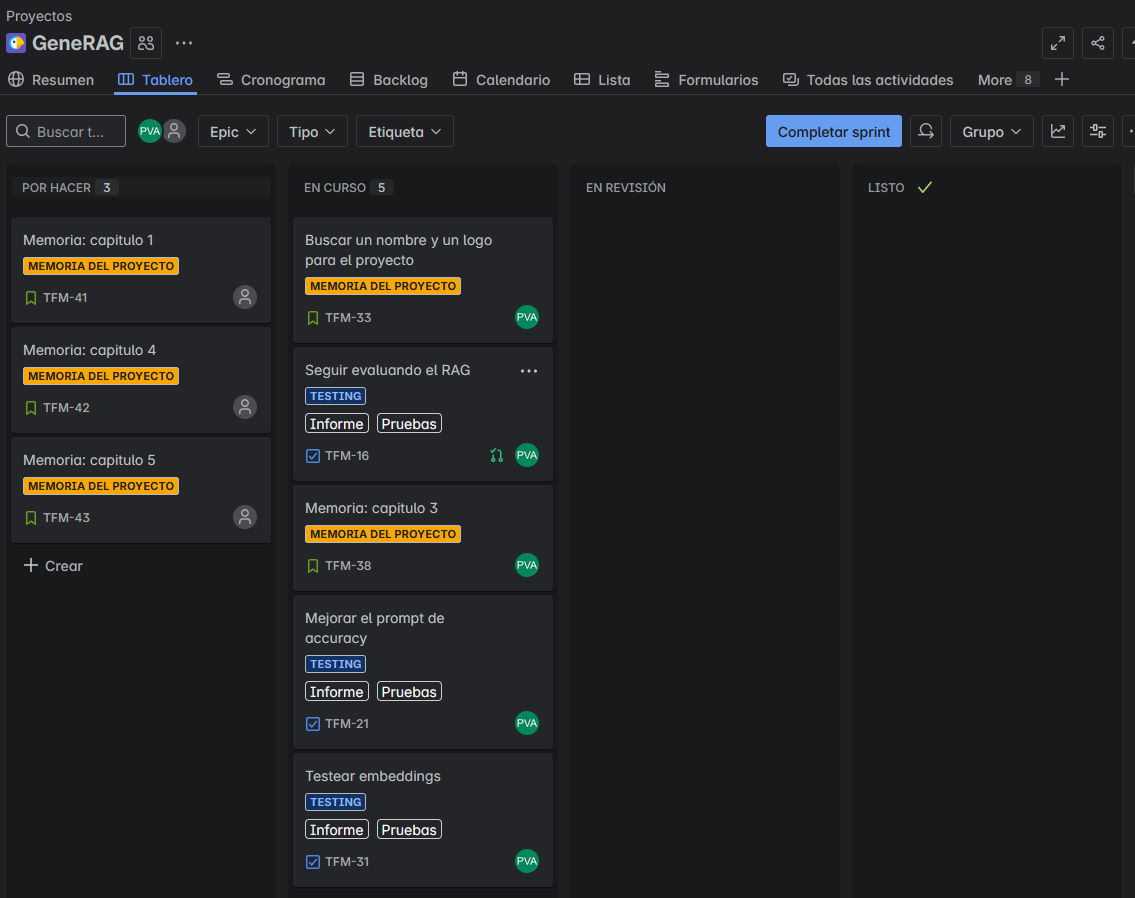
\includegraphics[width=0.8\textwidth]{imagenes/0058_jira-sprint2.png}
	            \caption{Jira. Tablero con tareas}		
	            \label{fig:0058_jira-sprint2}
	        \end{figure}         
	        
	        \noindent Por último, podemos ver el progreso en el tiempo de nuestro proyecto en la pestaña \textit{Cronograma} \cite{0056_proyectoJIRA}, el cual será explicado en la siguiente sección.
	        
      	\subsection{Fases del proyecto}      	  
      	
      		Las siguientes subsecciones explican brevemente lo realizado durante las distintas fases del proyecto, desde el inicio de la idea para el proyecto hasta su conclusión y entrega \cite{0056_proyectoJIRA}. En la figura \ref{fig:0139_crono}, observamos las fases por las que pasó el proyecto, su duración y los sprints totales. La duración total del proyecto ha sido de 204 días.     
      		
      		\begin{figure}[H]
      			\centering
      			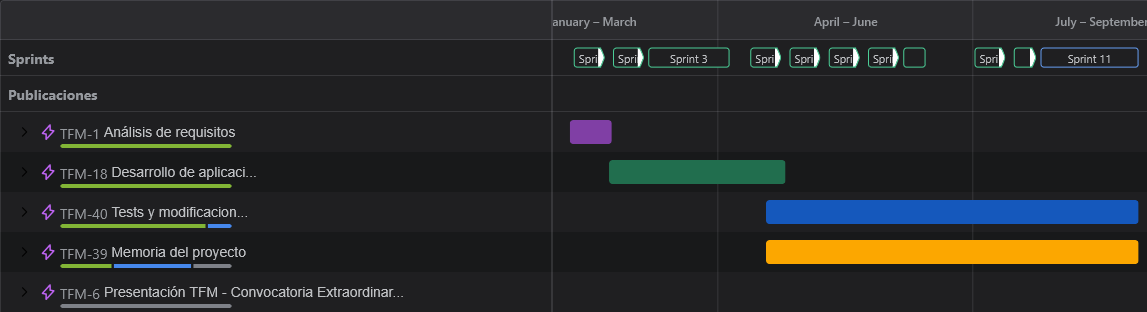
\includegraphics[width=1\textwidth]{imagenes/0139_crono.png}
      			\caption{Cronograma del proyecto. Extraído del proyecto en Jira \cite{0056_proyectoJIRA}}		
      			\label{fig:0139_crono}
      		\end{figure}          
        
        	\subsubsection{Fase 1: Análisis de requisitos} 
        	
        		En esta fase se presenta la idea del proyecto. Al principio, la idea era seguir experimentando con la plataforma RASA e iniciar un nuevo proyecto dedicado a crear un chatbot dedicado a un dominio en específico. 
        		
        		\noindent Pronto, la idea giró en torno a la utilización de los LLMs, dado a que era y es una tecnología en auge que presenta una mejora notable tanto en eficiencia como en rendimiento a lo que ofrece RASA en estos momentos. En este tiempo se realizaron varias demos usando las plataformas RASA y LangChain, decidiéndose por usar esta última en el proyecto.
        		
        		\noindent En la reunión que marcaba el final de sprint y de la fase, se determinó el propósito del chatbot: crear un asistente virtual capaz de responder con precisión y eficacia a cualquier pregunta relacionada con la DANA. Para ello, debíamos crear un RAG con los documentos del BOE relacionados con este tema. Además, nuestro tutor nos propuso la tarea de medir el grado de acierto del sistema RAG mediante el uso de agentes críticos. 
        		
        		\noindent Así pues, el proyecto quedó definido: crear un RAG sobre el contexto específico de la DANA, y medir su rendimiento evaluándolo a través de agentes críticos.
        		
        	\subsubsection{Fase 2: Desarrollo de la aplicación}
        	
        		En esta fase intermedia del proyecto, avanzamos en el desarrollo de la aplicación. Los cambios y adicciones al proyecto eran mostrados en las reuniones de finales de sprint, en las cuales se planteaban nuevas soluciones a las dificultades encontradas y se fijaban nuevos objetivos para el siguiente sprint. En esta etapa se completo el sistema RAG desde cero, desarrollo que se describe a continuación.
        		
        		\noindent El primer escollo, fue conseguir la fuente de conocimiento. Gracias a que los documentos del BOE se pueden conseguir vía API, se facilitó este primer problema. Fueron diseñados varios scripts para conseguir de forma automática estos documentos, y con la ayuda de \textit{GitHub Actions}, fueron programados para ejecutarse una vez al día salvo los domingos. De esta forma, obtuvimos la fuente de conocimiento que necesitaba nuestro RAG.
        		
        		\noindent La creación del RAG no tuvo mucha complicación debido a la gran cantidad de tutoriales y la versatilidad que nos permite LangChain en este contexto. La primera versión sin interfaz, era totalmente funcional en apenas unos días.
        		
        		\noindent En la interfaz empleamos más tiempo, dado a que la librería usada (Streamlit) ofrece bastantes elementos de personalización. La versión final permite cambiar el modelo de lenguaje usado para generar la respuesta, y también, elegir la estrategia de búsqueda empleada por el modelo de recuperación. En la parte de creación y actualización de la base de conocimientos, usamos dos alternativas para subir documentos desde la propia interfaz: desde carpeta o desde ficheros individuales.
        		
        		\noindent Completada esta fase, ya teníamos un sistema RAG totalmente funcional, con su fuente de conocimiento y una interfaz para responder consultas o añadir más documentos.
        		
        	\subsubsection{Fase 3: Test y modificaciones}
        	
        		Esta es la etapa de más duración del proyecto, y en la cual se realizaron todos los test para completar el segundo objetivo del trabajo.
        		
        		\noindent En primera instancia, desarrollamos un pequeño script diseñado para generar un conjunto de preguntas extraídas de nuestra fuente de conocimiento. Para su obtención, usamos el modelo de lenguaje Mistral Small 3.2, en el cual configuramos un prompt para este cometido. El conjunto de preguntas conseguido fue el usado para elaborar los test.
        		
        		\noindent Seguidamente, se preparó otro script en el que se configuró todo lo necesario para evaluar el RAG. Se definieron cuatro agentes críticos destinados a evaluar las métricas de \textit{accuracy}, \textit{faithfulnes}, \textit{groundedness} y \textit{relevancia}, es decir, el grado de similitud de la respuesta generada con la esperada, el uso de las evidencias proporcionadas por el modelo de recuperación en la respuesta generadas, y como de relevantes son los documentos recuperados para responder a la consulta.
        		
        		\noindent Las pruebas tomaron bastante tiempo debido al número realizado. Cada prueba de Mistral Small 3.2 empleaba alrededor de 3 horas en realizarse cuando el modelo estaba disponible, en ocasiones el servicio era más lento o fallaba. Llama 3.2 gastaba más o menos el mismo tiempo y GPT-4.1 era el más rápido (40 minutos), aunque para estos usamos conjuntos de pruebas más pequeños. Los resultados obtenidos fueron guardados y expuestos en tablas y gráficas, observables en el siguiente capítulo de esta memoria. 
        	
        	\subsubsection{Fase 4: Documentación}
        	
        		Esta fase se realizó en conjunto con la anterior (fase 3), por eso tiene más o menos la misma duración que esta. 
        		
        		\noindent En la estructura seguimos como guía la memoria usada en mi TFG, añadiendo y quitando las secciones que creímos necesarias.

        \subsection{Presupuesto}
        
        	En este apartado se describen los distintos recursos hardware y software empleados en el desarrollo del proyecto, explicando su uso y el coste de estos.
        	
        	\subsubsection{Recursos hardware}
        	
        		La tabla \ref{tab:rec_hard} muestra los recursos hardware usados. Para calcular el coste total de la tabla \ref{tab:presu_hard}, hemos dividido el precio entre la vida útil de cada dispositivo en días, para después multiplicarlo por el tiempo de realización del proyecto (204 días).
        		
        		\begin{table}[H]
        			\centering
        			\tiny
        			\begin{tblr}{
        					colspec = {p{2.5cm} p{3.5cm} p{7cm}},
        					row{1} = {bg=green!50}, 
        					hlines,
        					vlines,
        				}
        				\textbf{Dispositivo} & \textbf{Modelo} & \textbf{Uso} \\
        				Ordenador sobremesa & Ryzen5 3600 + 32GB RAM + 6700XT 12GB VRAM & Desarrollo y prueba de la aplicación \\
        				Ordenador portátil & Ryzen7 6800HS + 16GB RAM & Desarrollo y prueba de la aplicación \\        				
        			\end{tblr}
        			\caption{Recursos hardware utilizados}
        			\label{tab:rec_hard}
        		\end{table}
        		
        		\begin{table}[H]
        			\centering
        			\tiny
        			\begin{tblr}{
        					colspec = {p{6.5cm} p{2cm} p{2cm} p{2cm}},
        					row{1} = {bg=green!50}, 
        					row{4} = {bg=green!10}, 
        					hlines,
        					vlines,
        				}
        				\textbf{Modelo} & \textbf{Precio} & \textbf{Vida útil} & \textbf{Total} \\
        				Ryzen5 3600 + 32GB RAM + 6700XT 12GB VRAM & 1500€ & 8 años & 104.8€ \\
        				Ryzen7 6800HS + 16GB RAM & 1000€ & 6 años & 94.15€ \\     
        				\SetCell[c=3]{wd=10.5cm,valign=t}\textbf{Total} & & & \textbf{198.95€} \\		
        			\end{tblr}
        			\caption{Presupuesto de los recursos hardware utilizados}
        			\label{tab:presu_hard}
        		\end{table}
        		
        	\subsubsection{Recursos software}
        		
        		En este apartado se describen los recursos software utilizados, tanto su uso en la tabla \ref{tab:rec_soft}, como su precio en la tabla \ref{tab:presu_soft}. Los precios de estos recursos van ligados al coste de su licencia o uso.
        		
        		\begin{table}[H]
        			\centering
        			\tiny
        			\begin{tblr}{
        					colspec = {p{3cm} p{10cm}},
        					row{1} = {bg=green!50}, 
        					hlines,
        					vlines,
        				}
        				\textbf{Herramienta} & \textbf{Uso} \\
        				Windows 11 & Sistema Operativo \\    				
        				Visual Studio Code & Entorno de desarrollo \\
        				Ollama & Gestor de LLM y embeddings \\
        				LangChain & Librería control LLM \\
        				Streamlit & Librería interfaz \\
        				GitHub \& GitHub Actions & Plataforma donde esta el repositorio del proyecto, y plataforma para crear automatizaciones \\
        				Mistral API & Uso de LLMs de Mistral \\
        				OpenAI API & Uso de LLMs y embeddings de OpenAI \\
        				TexStudio & Procesador de látex usado para elaborar la memoria \\
        			\end{tblr}
        			\caption{Recursos software utilizados}
        			\label{tab:rec_soft}
        		\end{table}
        		
        		\begin{table}[H]
        			\centering
        			\tiny
        			\begin{tblr}{
        					colspec = {p{3cm} p{10cm}},
        					row{1} = {bg=green!50}, 
        					row{11} = {bg=green!10},
        					hlines,
        					vlines,
        				}
        				\textbf{Herramienta} & \textbf{Uso} \\
        				Windows 11 & 145€ \\    				
        				Visual Studio Code & Gratuito \\
        				Ollama & Gratuito \\
        				LangChain & Gratuito \\
        				Streamlit & Gratuito \\
        				GitHub \& GitHub Actions & Gratuito\\        				
        				Mistral API & Gratuito \\
        				OpenAI API & 12,79€ (15\$) \\
        				TexStudio & Gratuito \\
        				\textbf{Total} & \textbf{157.79€}
        			\end{tblr}
        			\caption{Presupuesto de los recursos software utilizados}
        			\label{tab:presu_soft}
        		\end{table}
        		
        	\subsubsection{Recursos personales}
        	
        		En este apartado describiremos los miembros presentes en la realización del proyecto. En la tabla \ref{tab:rec_ presu_pers} tendremos en cuenta el puesto, tiempo invertido y coste de ese tiempo. 
        		
        		\noindent Las horas realizadas por los tutores se han calculado teniendo en cuenta una media de una hora por reunión. De un total de 15 sesiones de reunión, disponemos de un total de 900 minutos o 15 horas. 
        		
        		\noindent El coste de su salario, se ha estimado sabiendo el salario bruto aproximado de un profesor de universidad (31500€ anuales, 24500€ netos según el IRPF de 2024). Por lo que, en un horario normal de 40 horas semanales, habiendo 4.34 semanas/mes , asciende a 11.76€ por hora. 
        		
        		\noindent Para el cómputo de mis horas, conociendo la duración del proyecto y en una media de 3 horas de trabajo al día, tenemos un total de 612 horas aproximadamente. El salario medio de un  programador junior ronda los 1500€, así que podemos estimar  un salario medio por hora de 8.64€, y un total de 5.287,68€.
        	
        		\begin{table}[H]
        			\centering
        			\tiny
        			\begin{tblr}{
        					colspec = {p{3cm} p{5.5cm} p{1cm} p{1cm} p{1cm}},
        					row{1} = {bg=green!50}, 
        					row{5} = {bg=green!10},
        					hlines,
        					vlines,
        				}
        				\textbf{Nombre} & \textbf{Puesto} & \textbf{Tiempo} & \textbf{Coste} & \textbf{Total}\\
        				David Griol Barres & Profesor de Universidad & 15h & 11.76€/h & 176.4€ \\
        				Zoraida Callejas Carrión & Profesor de Universidad& 15h & 11.76€/h & 176.4€ \\
        				Pablo Valenzuela Álvarez & Programador Junior & 612h & 8.64€ & 5.287,68€ \\
        				\SetCell[c=4]{wd=10.5cm,valign=t}\textbf{Total} & & & & \textbf{5.640,48€}\\
        			\end{tblr}
        			\caption{Presupuesto de los recursos personales utilizados}
        			\label{tab:rec_ presu_pers}
        		\end{table}
        	
        	\subsubsection{Coste total}
        	
        		Sumando todos los costes parciales del proyecto, tenemos un subtotal de 5.997,22€.
        		
        		\begin{table}[H]
        			\centering
        			\tiny
        			\begin{tblr}{
        					colspec = {p{6cm} p{7cm}},
        					row{1} = {bg=green!50}, 
        					row{5} = {bg=green!10},
        					hlines,
        					vlines,
        				}
        				\textbf{Tipo} & \textbf{Coste} \\
        				Coste del hardware & 198.95€ \\    				
        				Coste del software & 157.79€ \\    				
        				Coste del personal & 5.640,48€ \\    				
        				\textbf{Total} & \textbf{5.997,22€}
        			\end{tblr}
        			\caption{Coste total del proyecto}
        			\label{tab:presu_total}
        		\end{table}
        		
    \section{Construcción del corpus de documentos}

        La plataforma elegida para el control de versiones del proyecto fue \textit{GitHub}, ya que es la plataforma con la que llevamos años trabajando en proyectos anteriores y es la más implantada en el mercado. 
        
        \noindent A parte de dar un acceso rápido y seguro al código del repositorio, \textit{GitHub} ofrece una herramienta para controlar flujos de trabajo automáticos llamada \textbf{GitHub Actions}. Flujos que hemos usado para automatizar las descargas de los documentos usados para crear el corpus de información con la que hemos nutrido el modelo de recuperación de información de nuestro sistema RAG. Este es un concepto conocido como integración continua y entrega continua (\textit{CI/CD}).

        \noindent Como se ha mencionado en anteriores apartados, hemos usado documentos del BOE (Boletín Oficial del Estado) relacionados con la DANA para construir nuestro corpus de conocimiento. Desde la propia web del BOE, podemos acceder a los sumarios de cada día mediante descarga gracias a una API.       

        \begin{figure}[H]
            \centering
            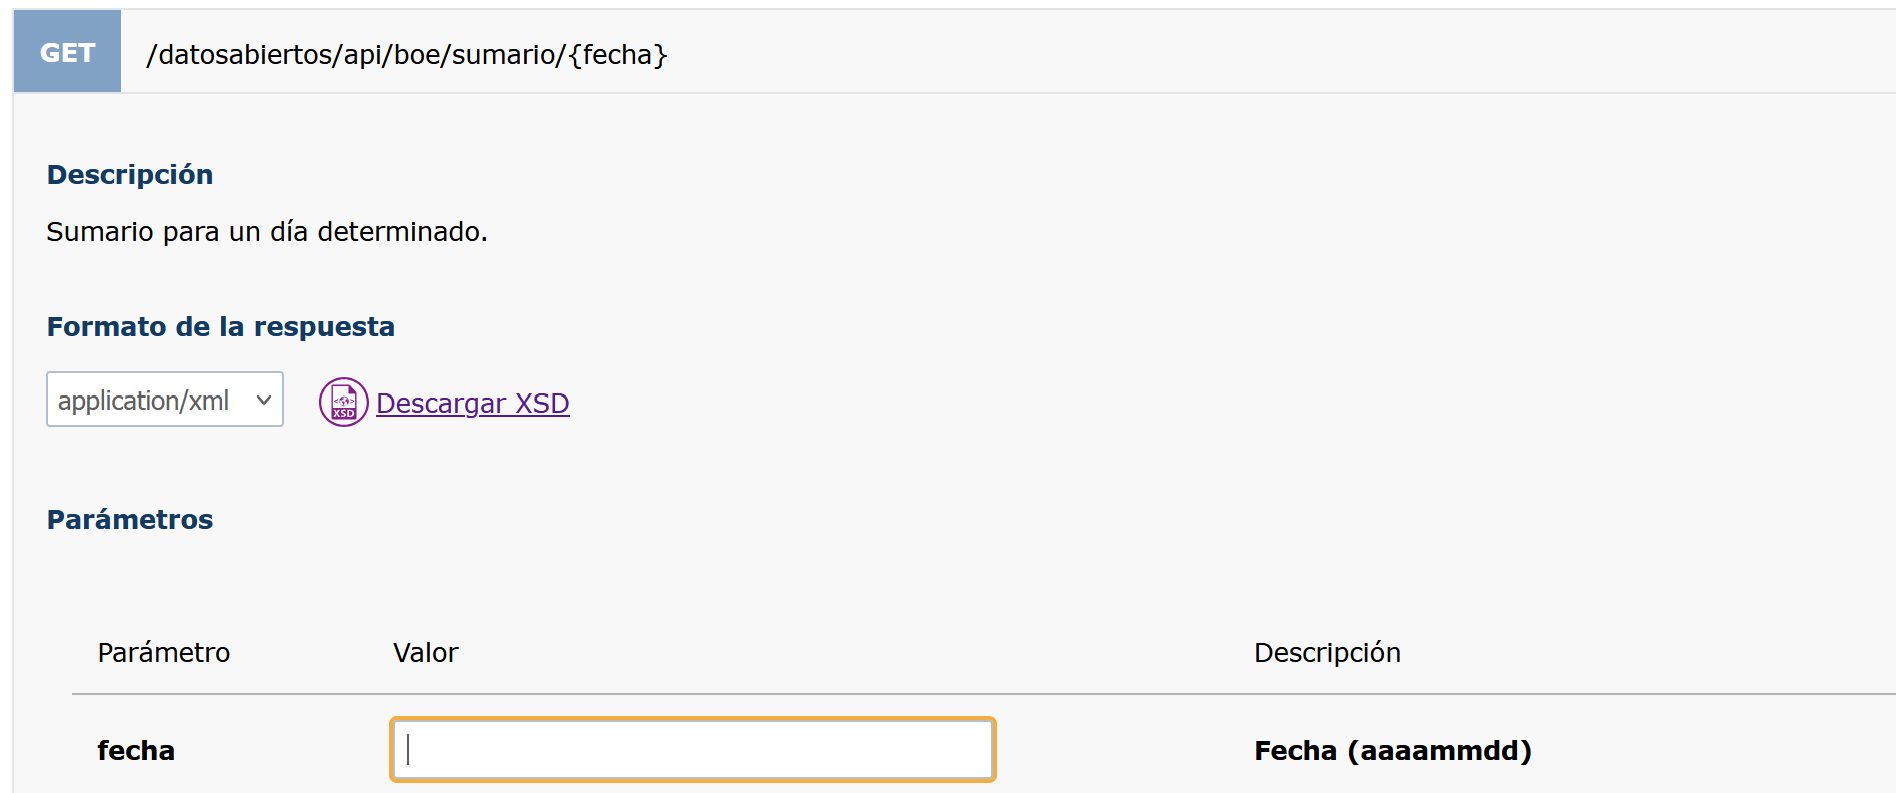
\includegraphics[width=1\textwidth]{imagenes/0059_boe_api.png}
            \caption{BOE. API web desde la que descargar sumarios por día \cite{0029_boe_api}}		
            \label{fig:0059_boe_api}
        \end{figure} 

        \begin{figure}[H]
            \centering
            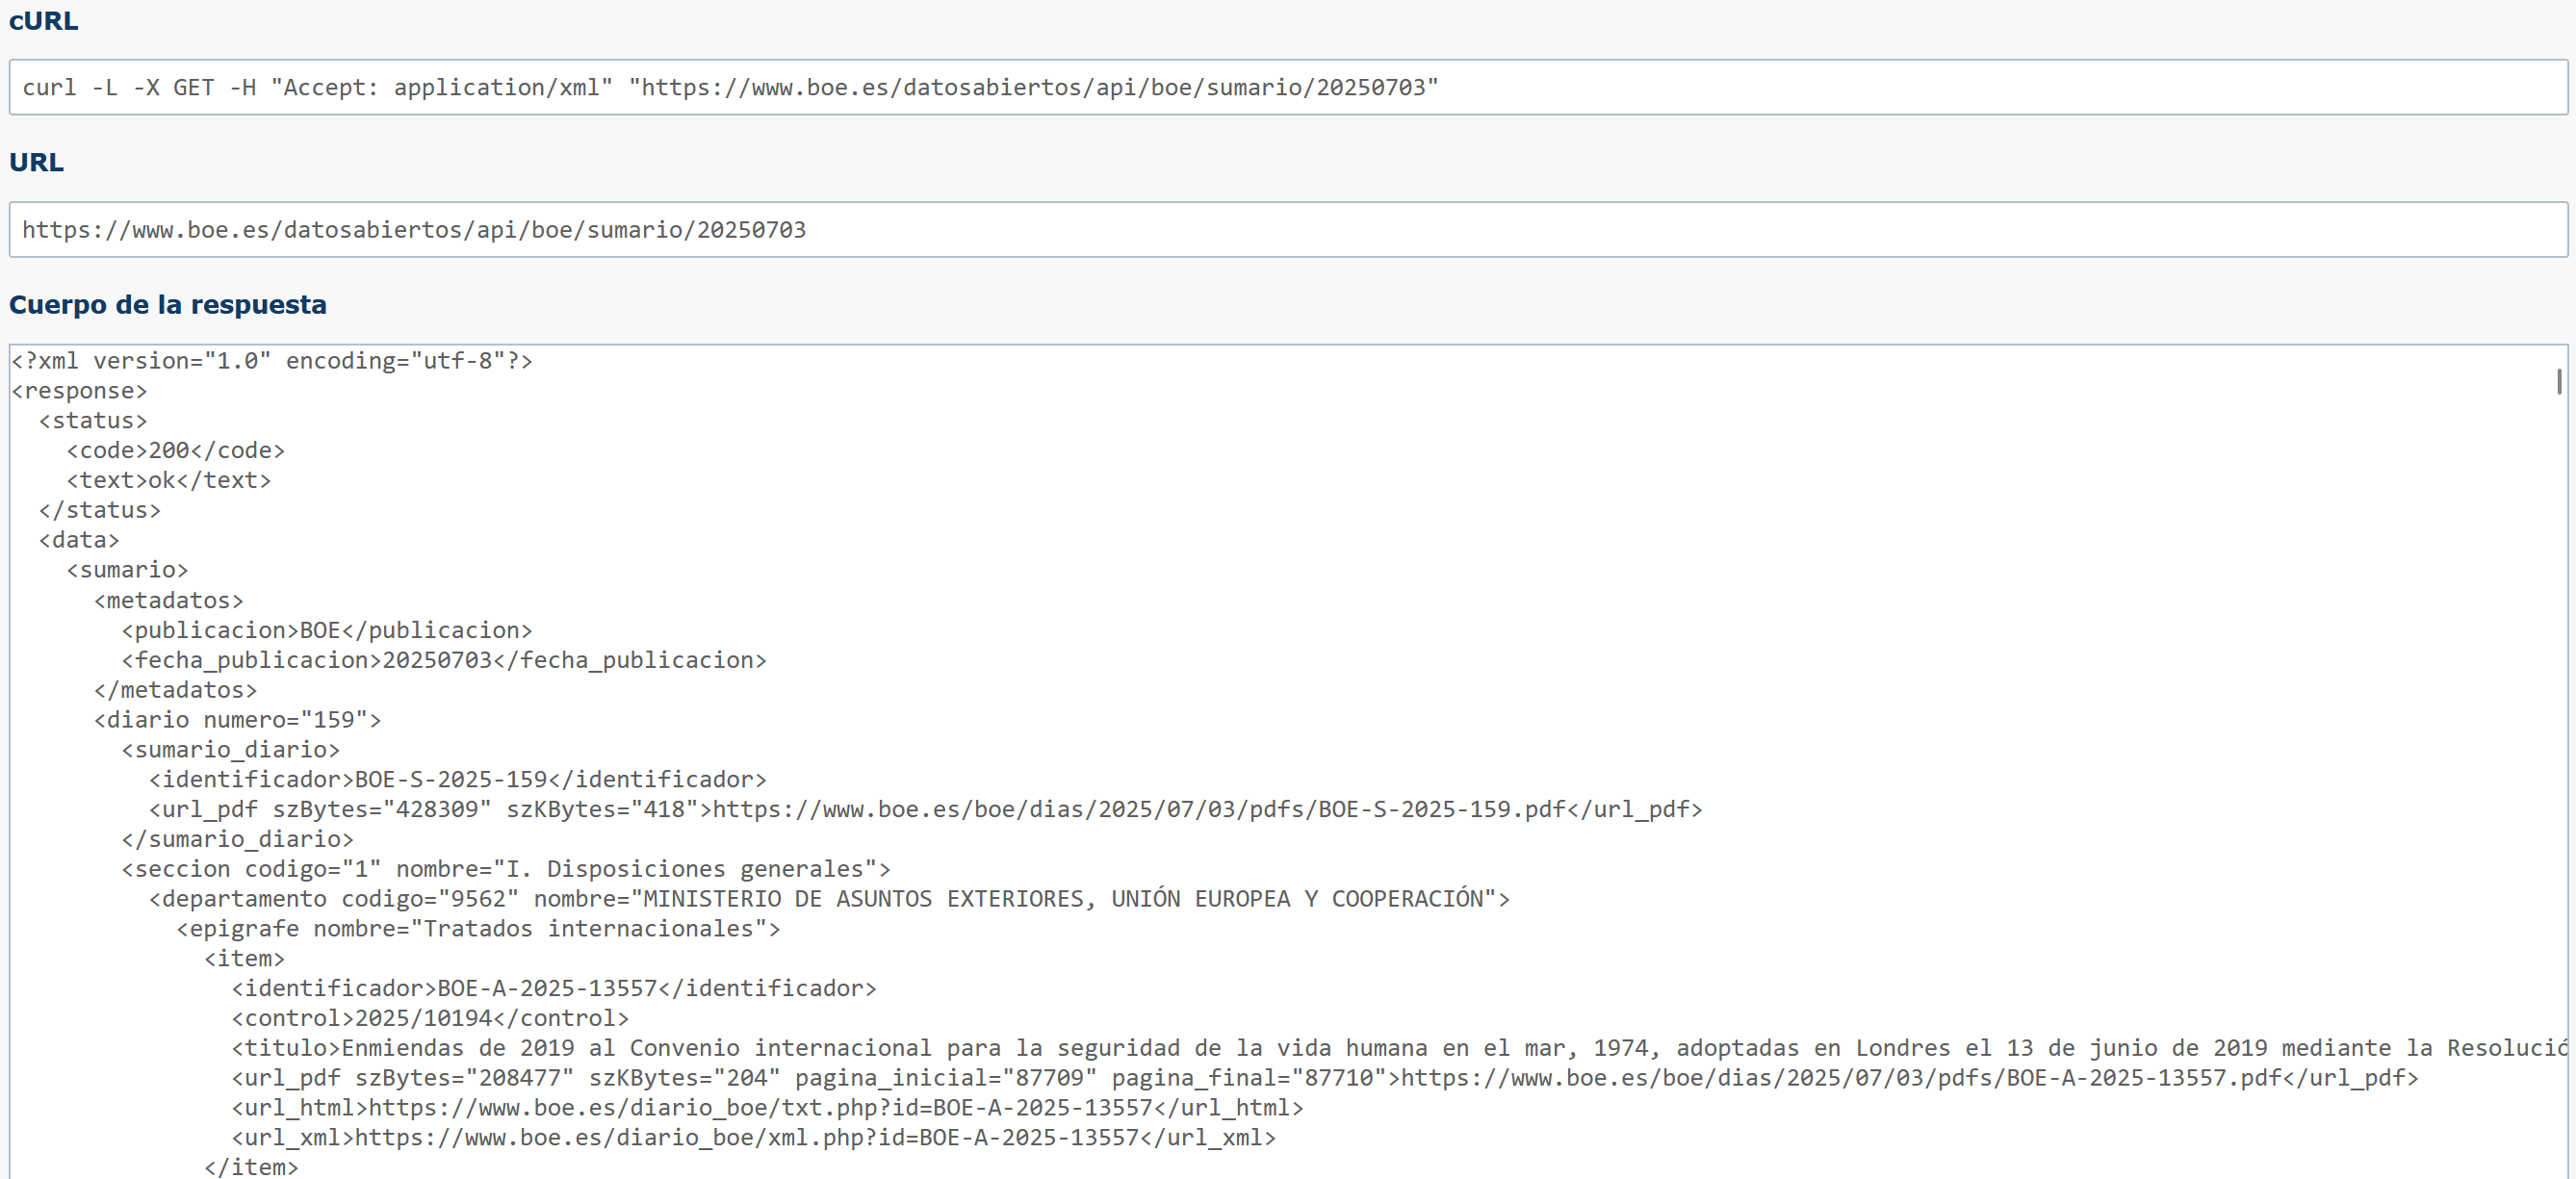
\includegraphics[width=1\textwidth]{imagenes/0060_boe_api2.png}
            \caption{BOE. Resultados de la búsqueda de un día \cite{0029_boe_api}}		
            \label{fig:0060_boe_api2}
        \end{figure} 

        \noindent Esta API nos ofrece dos opciones de descarga para el sumario: json y xml. En la figura \ref{fig:0060_boe_api2} podemos ver la versión xml de la descarga.

        \noindent El requerimiento para la obtención del sumario es la fecha redactada en un formato \textbf{aaaammdd}, es decir, si queremos obtener el sumario del día 30 de mayo de 2025, tenemos que redactarlo de la siguiente manera: 20250530.

        \subsection{Script de descarga de sumarios}
        \label{subsec:3_script_suma}

            La fecha del sistema es fácil de obtener mediante código, por dicha razón se implementaron dos scripts: uno para la descarga automática del sumario del día actual y otro para la descarga de sumarios de días anteriores, necesarios para el paso siguiente (ver sección \ref{subsec:3_script_docs}).
    
            \begin{figure}[H]
                \centering
                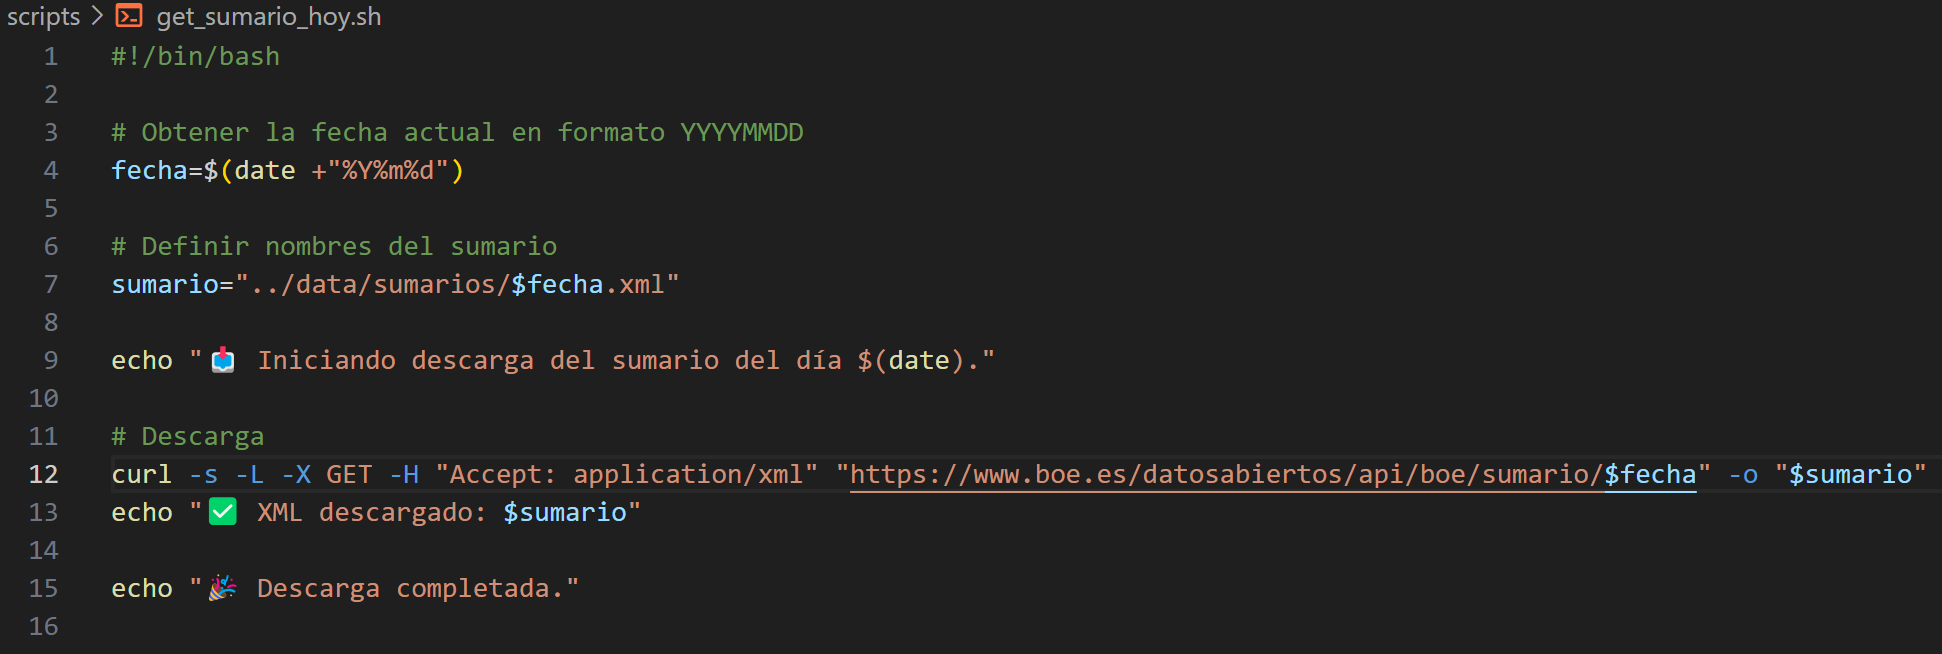
\includegraphics[width=0.9\textwidth]{imagenes/0061_get_sumario.png}
                \caption{Script para descargar el sumario del día}		
                \label{fig:0061_get_sumario}
            \end{figure} 
    
            \noindent Como se observa en la figura \ref{fig:0061_get_sumario}, se obtiene la fecha del sistema automáticamente y se usa tanto para la llamada a la API como para guardar el documento descargado. Este script es el se usó posteriormente para crear hacer una automatización por medio de GitHub Actions (ver sección \ref{subsec:3_subsec_auto}).

        \subsection{Script para la descarga de documentos}
        \label{subsec:3_script_docs}

            Los sumarios en su estructura xml contienen varias etiquetas que podemos usar para buscar y descargar los documentos que nos interesen. Como podemos observar en la figura \ref{fig:0060_boe_api2}, la etiqueta \textit{item} engloba tanto las etiquetas del título como varias etiquetas de descargas. Ayudándonos de estas etiquetas, se optó por crear un script en Python que automatizase el proceso de descarga de los documentos relacionados con la DANA.

            \noindent El funcionamiento de este script es el siguiente:

            \begin{itemize}
                \item Recorremos en bucle todas las etiquetas ``\textit{item}"
                \item Para cada etiqueta ``\textit{item}" se guardan en variables: título y enlace de descarga pdf.
                \item Se comprueba si el título contiene la palabra ``DANA".
                \item Se descarga el documento gracias a la etiqueta del enlace pdf.
            \end{itemize}     

            \noindent En la figura \ref{fig:0062_get_docs} se puede observar este procedimiento.
    
            \begin{figure}[H]
                \centering                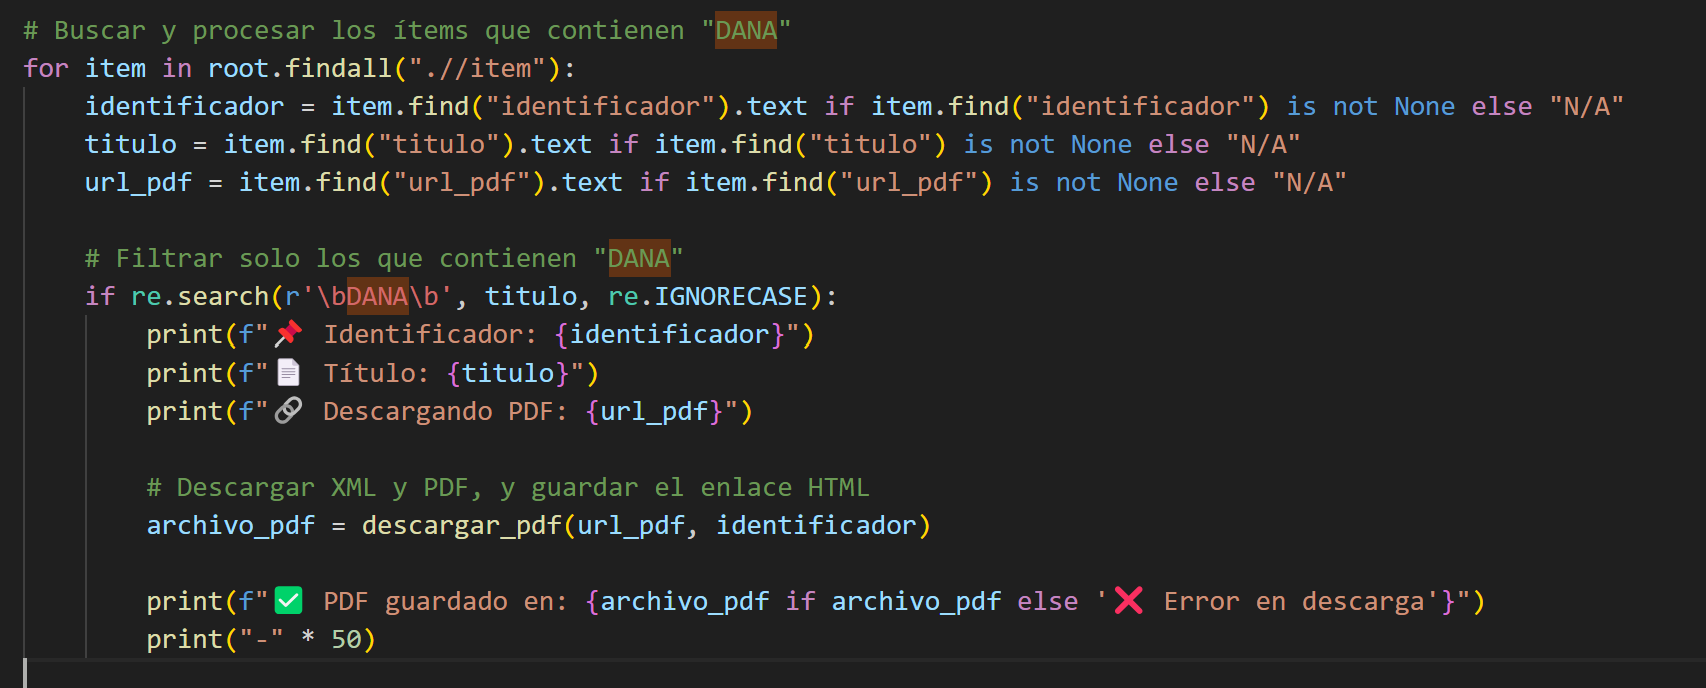
\includegraphics[width=0.8\textwidth]{imagenes/0062_get_docs.png}
                \caption{Fragmento del script encargado de obtener documentos relacionados con la DANA}		
                \label{fig:0062_get_docs}
            \end{figure} 

            \noindent Como sucedió en el apartado anterior, se hizo necesaria la implementación de otro script para la descarga de los documentos de días anteriores. El procedimiento es el mismo que el visto en la figura \ref{fig:0062_get_docs}, añadiendo un bucle extra en el cual recorre todos los sumarios descargados. 
            
            \noindent Tanto estos como los scripts del apartado anterior, están disponibles en la carpeta \textbf{scripts} del repositorio \cite{0045_repo} en \textit{GitHub}.

        \subsection{Automatización de procesos de descarga}
        \label{subsec:3_subsec_auto}

            Una vez implementados los scripts para la descarga de sumarios y de documentos, llega la hora de crear la automatización en GitHub. Para ello usaremos la herramienta para crear acciones: \textit{GitHub Actions}.

            \noindent \textit{GitHub Actions} es una plataforma de integración y despliegue continuos (\textit{CI/CD}) que permite la automatización de flujos de trabajo \cite{0030_gh_actions}.
    
            \begin{figure}[H]
                \centering
                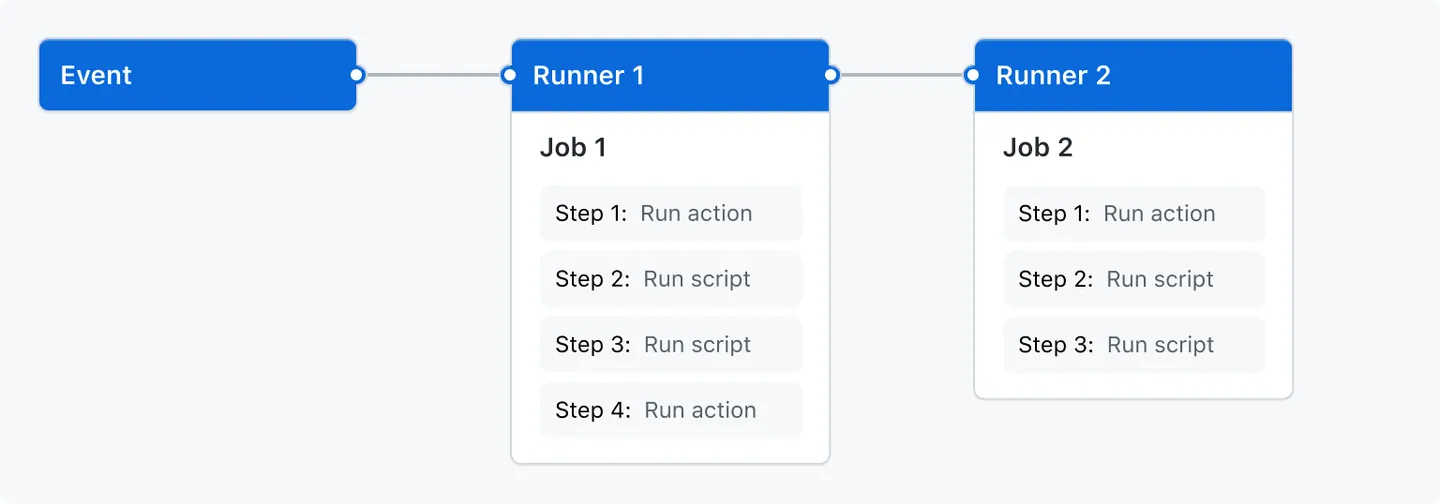
\includegraphics[width=0.8\textwidth]{imagenes/0063_ghact_fun.png}
                \caption{GitHub Actions. Ejemplo de funcionamiento de un flujo de trabajo \cite{0030_gh_actions}}		
                \label{fig:0063_ghact_fun}
            \end{figure} 

            \noindent Como se observa en la figura \ref{fig:0063_ghact_fun}, un flujo de trabajo (\textit{workflow}) se activa cuando sucede un evento (\textit{event}) en el repositorio: \textit{push}, \textit{commit}, etc. Cada trabajo (\textit{job}) ejecuta uno o varios scripts en una máquina virtual creada automáticamente que se elimina al completar los procesos del flujo de trabajo.

            \noindent Los flujos de trabajo son procesos automatizados y configurables definidos por un fichero \textit{YAML} ubicado en el directorio \textit{.github/workflow} de nuestro repositorio \cite{0045_repo}. Nuestro objetivo es que el flujo de trabajo se ejecute una vez al día, exceptuando los domingos (no se publica el BOE los domingos); y que ejecute ambos scripts vistos en las dos secciones anteriores.

            \noindent En este sentido, tenemos que configurar un evento que haga que se ejecute todos los días exceptuando el domingo. Esto se logra usando el comando \textit{cron} como se muestra en la figura \ref{fig:0064_ghact_cron}. En dicha figura, se programa para ejecutarse de lunes a sábado a las 9:00 de la mañana, sin importar día o mes.
    
            \begin{figure}[H]
                \centering
                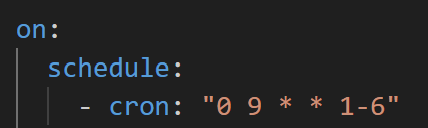
\includegraphics[width=0.4\textwidth]{imagenes/0064_ghact_cron.png}
                \caption{GitHub Actions. Fragmento del flujo de trabajo que muestra el uso del comando cron}		
                \label{fig:0064_ghact_cron}
            \end{figure}

            \noindent Tras programar el evento que activa el flujo de trabajo, solo queda indicar las tareas que se ejecutarán en el flujo. En la figura \ref{fig:0065_ghact_jobs} se pueden observar estas tareas bajo la etiqueta \textit{steps}, estos son iniciadas secuencialmente como indica la figura. En las primeras líneas, indica sobre que sistema se esta ejecutando: una máquina virtual Ubuntu.
    
            \begin{figure}[H]
                \centering
                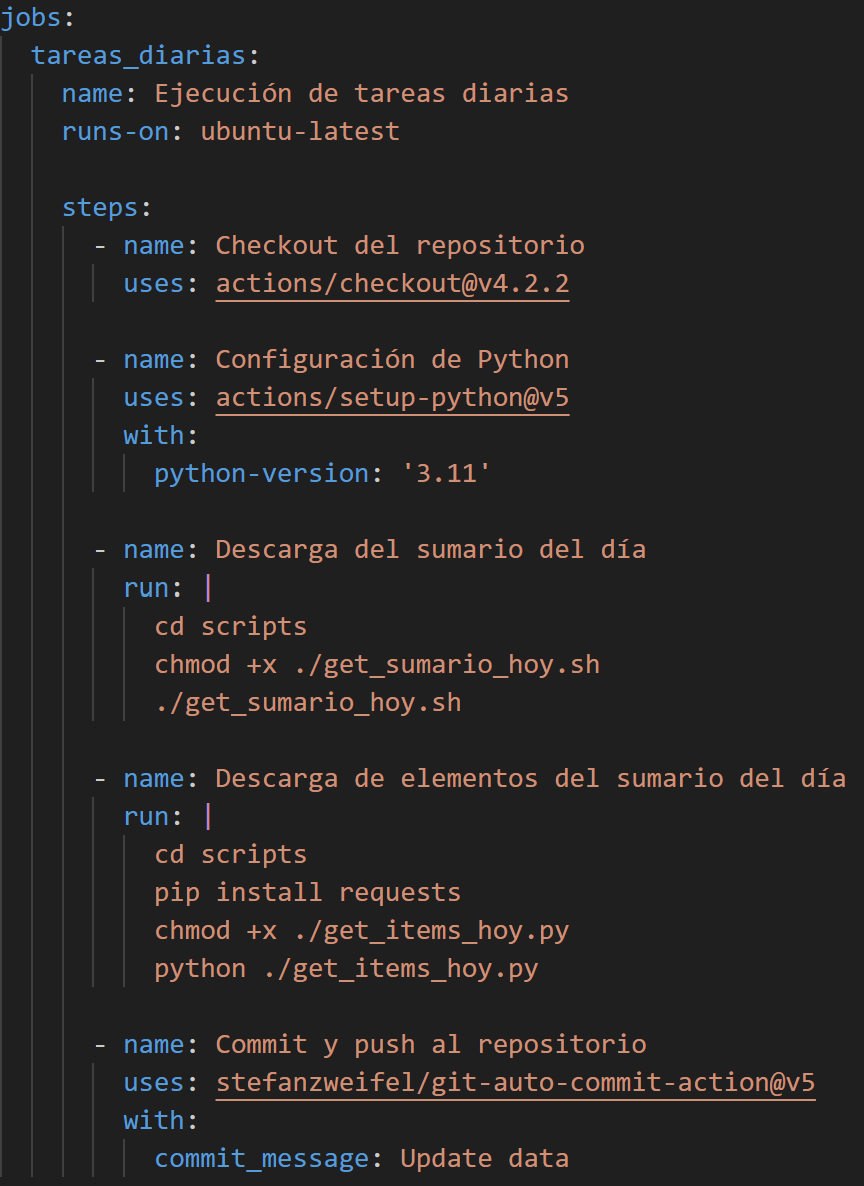
\includegraphics[width=0.5\textwidth]{imagenes/0065_ghact_jobs.png}
                \caption{GitHub Actions. Fragmento del flujo de trabajo que muestran los trabajos que son ejecutados}		
                \label{fig:0065_ghact_jobs}
            \end{figure}

            \noindent La lista siguiente contiene una breve descripción de cada una de las tareas del flujo por sus nombres:

            \begin{enumerate}
                \item \textbf{Checkout del repositorio}: Es una acción creada por la comunidad que clona el repositorio en la máquina virtual. 
                \item \textbf{Configuración de Python}: Utiliza otra acción creada por la comunidad, se encarga de instalar un entorno \textit{Python} en la máquina virtual.
                \item \textbf{Descarga del sumario del día}: Lanza el script de descarga del sumario del día (sección \ref{subsec:3_script_suma}).
                \item \textbf{Descarga de elementos del sumario del día}: Lanza el script de descarga de documentos del sumario del día relacionados con la DANA (sección \ref{subsec:3_script_docs}).
                \item \textbf{Commit y push al repositorio}: Ultiliza la acción \textit{auto-commit}, creada por la comunidad. Como su nombre indica, se encarga de actualizar los sumarios y documentos descargados, si hay nuevos.
            \end{enumerate}

            \noindent Para finalizar la subsección, queda comprobar si la acción se esta lanzando correctamente. Podemos obtener esta información en la pestaña ``Acciones" de la página web de \textit{GitHub} de nuestro repositorio \cite{0045_repo}. En las figuras siguientes podemos observar el funcionamiento de las acciones en el repositorio del proyecto \cite{0045_repo}.          
    
            \begin{figure}[H]
                \centering
                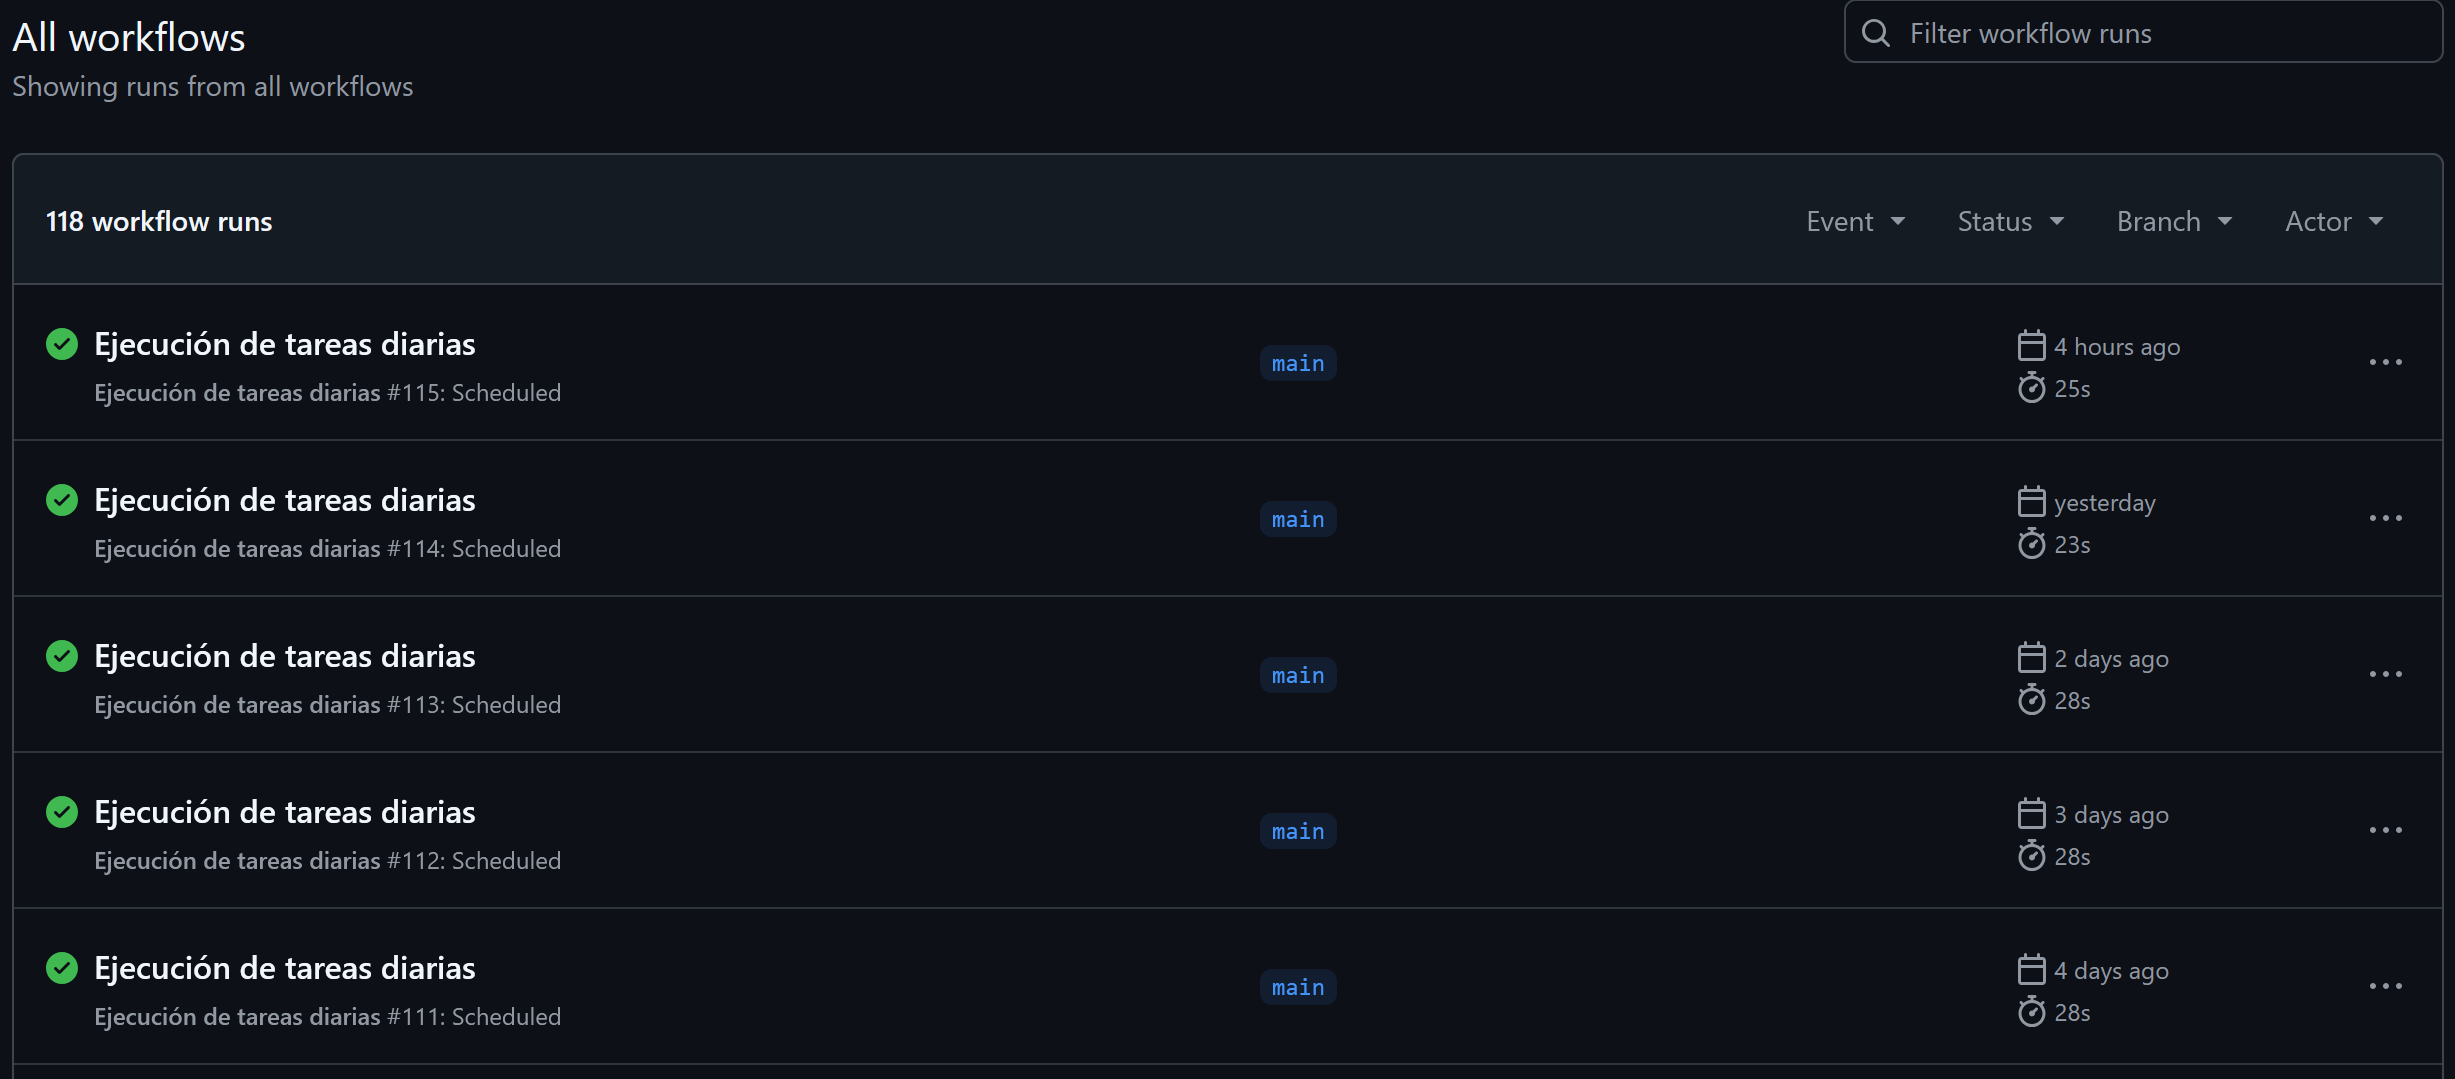
\includegraphics[width=0.8\textwidth]{imagenes/0066_ghact_allwf.png}
                \caption{Pestaña de acciones del proyecto. Se muestran una parte de las acciones automatizadas}		
                \label{fig:0066_ghact_allwf}
            \end{figure}        

            \noindent Podemos comprobar en la figura \ref{fig:0066_ghact_allwf} como, efectivamente, las acciones de lanzan una vez al día.
    
            \begin{figure}[H]
                \centering
                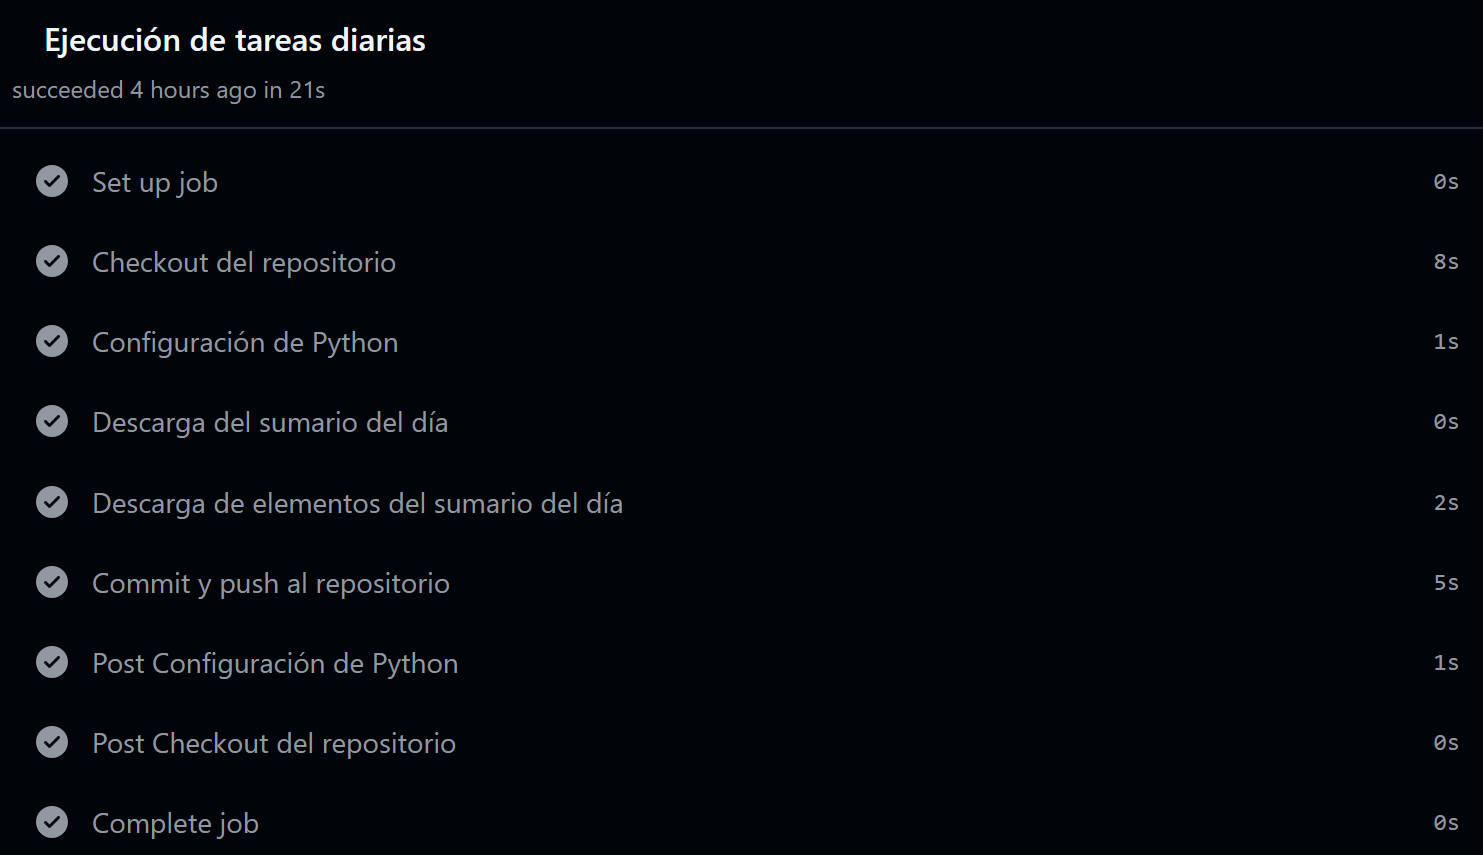
\includegraphics[width=0.8\textwidth]{imagenes/0067_ghact_finfin.png}
                \caption{Vista en detalle de una acción. Se observa el tiempo empleado en realizar cada paso}		
                \label{fig:0067_ghact_finfin}
            \end{figure}

            \noindent En la vista en detalle aportada en la figura \ref{fig:0067_ghact_finfin}, podemos entender como funciona internamente una acción, siguiendo los pasos indicados en el fichero \textit{YAML}. Los procesos \textit{post} se encargan de deshacer los procesos de \textit{checkout} y configuración de \textit{Python}, para terminar liberando la máquina virtual en el último paso. 

            \noindent De esta manera, hemos logrado crear una base de conocimiento con documentos del BOE relacionados con la DANA, y que es actualizada diariamente.

    \section{Desarrollo del chatbot}

        Esta sección contará los pasos que hemos seguido en el desarrollo de la aplicación chatbot que tiene de base nuestro sistema RAG. Encontraremos apartados dedicados tanto al desarrollo de la interfaz web como al de los diferentes componentes que configuran nuestro sistema RAG, incluyendo imágenes con fragmentos de código y de la interfaz final.

        \noindent El objetivo es crear una interfaz en la cuál: podamos añadir nuevos documentos a nuestro sistema RAG y, evidentemente, un chatbot con el que podamos comunicarnos, y que utilice documentos recuperados del RAG para construir su respuesta. Para dicho cometido se implemento una clase \textit{chatbot} (ubicada dentro de la carpeta \textit{classes} del repositorio \cite{0045_repo}), que contiene los métodos necesarios para hacer un funcionar el sistema RAG completo. 

        \noindent En las siguientes subsecciones mostraremos la implementación de estos procesos: la configuración, carga y agregación de nuevos documentos a la base de datos vectorial, y la recuperación y generación de información; todo ejemplificándolo con fragmentos de código representativos y muestras del resultado en la interfaz web.

        \subsection{Clase Chatbot: constructor}

            El constructor de la clase \textit{Chatbot}, como se observa en la figura \ref{fig:0068_chatbot_const_1}, contiene una gran cantidad de parámetros. Con ello podemos configurar desde la inicialización todos los aspectos necesarios del sistema RAG propuesto.

            \begin{figure}[H]
                \centering
                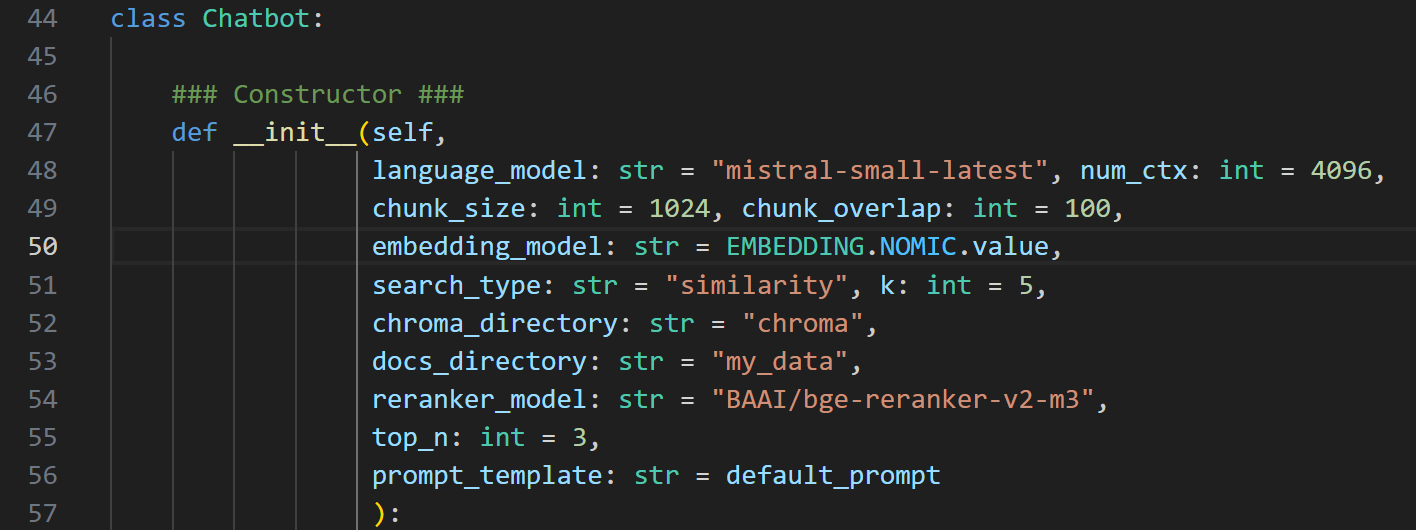
\includegraphics[width=1\textwidth]{imagenes/0068_chatbot_const_1.png}
                \caption{Clase Chatbot. Parámetros del constructor}		
                \label{fig:0068_chatbot_const_1}
            \end{figure}

            \noindent En la siguiente lista, vamos a explicar cada uno de los parámetros:

            \begin{itemize}
                \item \textbf{language\_model:} Indica el modelo de lenguaje (LLM) que usaremos para generar la respuesta.
                \item \textbf{num\_ctx:} Ventana de contexto que usa el LLM, es decir, la cantidad de información aportada al LLM mediante el prompt.
                \item \textbf{chunk\_size y chunk\_overlap:} Parámetros usados para separar y solapar documentos a la hora de añadirlos al RAG.
                \item \textbf{embedding\_model:} Modelo de embedding usado por el RAG, también es usado en las consultas de usuario.
                \item \textbf{search\_type y k:} Estrategia de búsqueda usada al recuperar información. La cantidad de documentos recuperados la indica k.
                \item \textbf{chroma\_directory:} Localización del modelo de recuperación (base de datos vectorial).
                \item \textbf{docs\_directory:} Localización del corpus usado, que nutre la base de datos vectorial.
                \item \textbf{reranker\_model y top\_n:} Modelo utilizado para hacer reranking sobre los documentos recuperados. La cantidad de documentos filtrados por el reranker la indica top\_n.
                \item \textbf{prompt\_template:} Plantilla de texto utilizada para generar la respuesta.
            \end{itemize}

            \noindent Como se observa en la imagen anterior cada parámetro usa valores por defecto, de esta manera se facilita el uso de esta clase. Cada uno de estos parámetros son editables en todo momento, puesto que se han incluido métodos \textit{GET} y \textit{SET} para estos cometidos.

            \noindent A continuación veremos en las figuras retazos de la configuración de alguno de ellos. Como por ejemplo la figura \ref{fig:0069_chatbot_const_2}, donde se muestra la configuración del modelo de lenguaje según sea el seleccionado. Hasta ahora contamos con el modelo \textit{mistral-small} correspondiente a MistralAI, \textit{GPT-4.1} de OpenAI y Llama3.2 perteneciente a Ollama, por lo que necesitamos diferentes clases para que funcionen: ChatMistralAI, ChatOpenAI y ChatOllama. En los modelos proporcionados por Mistral AI y OpenAI necesitamos facilitar la clave de su API.

            \begin{figure}[H]
                \centering
                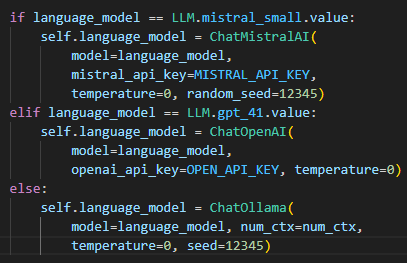
\includegraphics[width=0.6\textwidth]{imagenes/0069_chatbot_const_2.png}
                \caption{Clase Chatbot. Configuración del LLM}		
                \label{fig:0069_chatbot_const_2}
            \end{figure}

            \noindent En cuanto a la configuración del modelo de recuperación, la figura \ref{fig:0070_chatbot_const_3} muestra su implementación. La separación de documentos es efectuada mediante el uso de la clase \textit{RecursiveTextSplitting} \cite{0031_langchain_recursiveCS}, que se encarga de separar los documentos dado un determinado tamaño del chunk (\textit{chunk\_size}). El solapamiento se controla con \textit{chunk\_overlap}, este ayuda a mantener una relación semántica entre documentos similares o consecutivos.

            \noindent La figura \ref{fig:0070_chatbot_const_3} también muestra como se configura el modelo de embedding y la base de datos vectorial (\textit{vector\_store}); utilizando sendas clases \textit{OllamaEmbeddings} y \textit{Chroma} para realizar estas acciones. En el caso de usar un modelo de embedding proviniente de OpenAI, tenemos que usar la clase \textit{OpenAIEmbeddings} que ofrece LangChain.

            \begin{figure}[H]
                \centering
                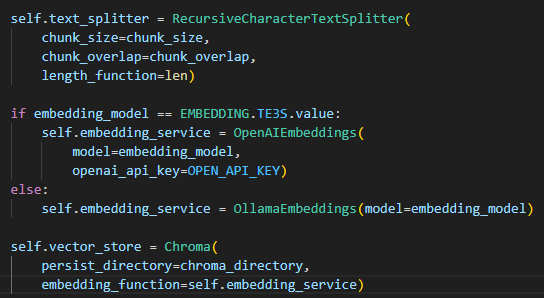
\includegraphics[width=0.8\textwidth]{imagenes/0070_chatbot_const_3.png}
                \caption{Clase Chatbot. Configuración de varios parámetros: text\_splitter, modelo de embedding y modelo de recuperación}		
                \label{fig:0070_chatbot_const_3}
            \end{figure}

            \noindent La configuración de la estrategia de búsqueda no es tan simple, en la figura \ref{fig:0071_chatbot_const_4} podemos ver las opciones de configuración disponibles. Mientras que métodos como \textit{Similarity} o \textit{MMR} están incluidas por defecto por Chroma, necesitamos usar clases específicas para las demás.

            \noindent Las estrategias \textit{TF-IDF} y \textit{BM25} utilizan una metodología distinta, por lo que necesitan el uso de las clases \textit{TFIDFRetriver} \cite{0032_tfidf} y \textit{BM25Retriever} \cite{0033_bm25} para funcionar correctamente.

            \noindent La estrategia de recuperación en grafo usa la clase \textit{GrapRetriever} \cite{0034_graphrag}, en la que usamos algunos metadatos obtenidos de los documentos para filtrar y recuperar documentos con metadatos similares.

            \begin{figure}[H]
                \centering
                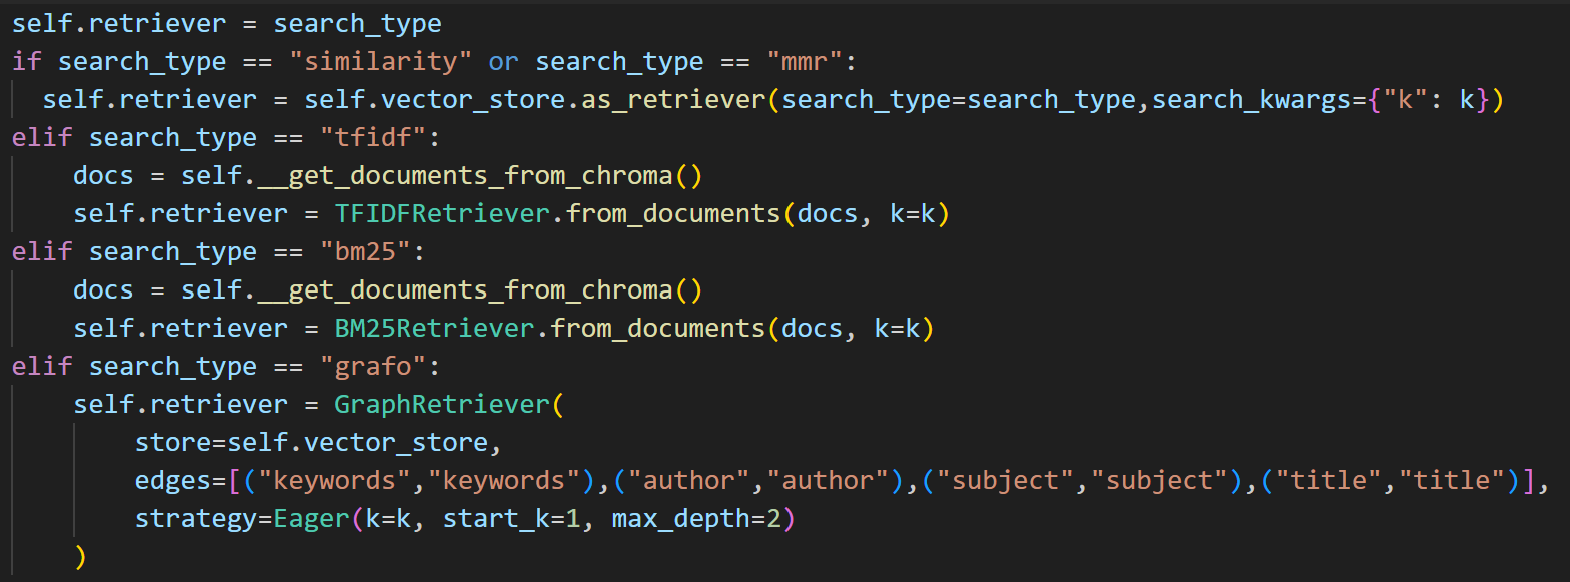
\includegraphics[width=1\textwidth]{imagenes/0071_chatbot_const_4.png}
                \caption{Clase Chatbot. Configuración de la estrategia de búsqueda}		
                \label{fig:0071_chatbot_const_4}
            \end{figure}

            \noindent La especificación del prompt es sencilla y se puede implementar en una sola línea (figura \ref{fig:0072_chatbot_const_5}. La clase \textit{PromptTemplate} ofrece multitud de métodos para este fin. El contenido de la variable \textit{prompt\_template} se puede ver al final de la sección \ref{sec:interfaz_chatbot} de esta memoria.

            \begin{figure}[H]
                \centering
                
\includegraphics[width=0.8\textwidth]{imagenes/0072_chatbot_const_5.png}
                \caption{Clase Chatbot. Configuración del prompt}		
                \label{fig:0072_chatbot_const_5}
            \end{figure}

            \noindent La última de las configuraciones corresponde a la del modelo para hacer \textbf{reranking} (figura \ref{fig:0073_chatbot_const_6}). Para ello necesitamos usar varias clases, y como parámetros: el modelo de reranking y el número de documentos que filtrará (\textit{top\_n}). 

            \noindent La variable \textit{compressor\_retriever} guarda la configuración del modelo de reranking junto con el modelo de recuperación escogido para esta iteración del sistema RAG. De modo que al llamarla, se producirá un ``doble" filtrado de los documentos: primero se producirá la recuperación de documentos normal, y seguido, el filtrado de los mejores documentos recuperados por parte del modelo reranker.

            \begin{figure}[H]
                \centering
                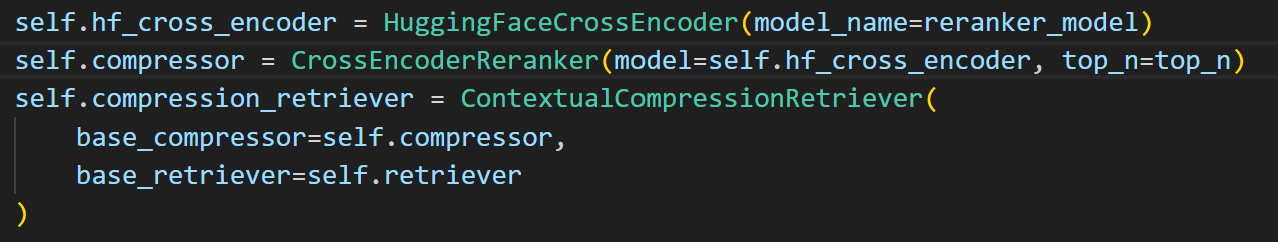
\includegraphics[width=0.9\textwidth]{imagenes/0073_chatbot_const_6.png}
                \caption{Clase Chatbot. Configuración del reranker}		
                \label{fig:0073_chatbot_const_6}
            \end{figure}

            \noindent Hemos podido ver en las figuras anteriores, la cantidad de integraciones que hemos usado para la configuración de los diferentes elementos de la clase \textit{Chatbot}. Como ya comentamos en la sección \ref{sec:LangChain}, esta es la gran ventaja que ofrece \textit{LangChain} respecto a otros frameworks, y que tenemos que aprovechar para facilitar el desarrollo de cualquier proyecto.

        \subsection{Interfaz de carga y actualización de la base de datos}

            En este apartado veremos como cargar y actualizar la base de datos vectorial del sistema RAG. Las siguientes imágenes, muestran fragmentos del código utilizado para su implementación. 

            \noindent En la siguiente figura podemos ver como se implementa parte de la interfaz usando \textit{Streamlit}. Hemos marcado tres bloques en la figura que pasaremos a explicar a continuación.

            \begin{figure}[H]
                \centering
                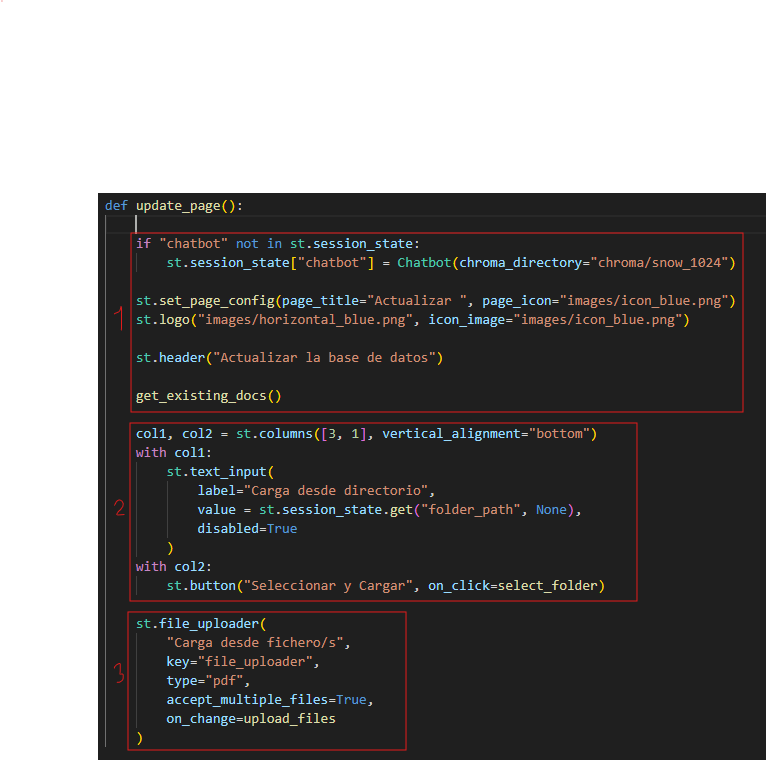
\includegraphics[width=1\textwidth]{imagenes/0074_update1.png}
                \caption{Interfaz. Código de la página de carga y actualización de la base de datos}		
                \label{fig:0074_update1}
            \end{figure}

            \noindent El primer bloque contiene la inicialización del \textit{Chatbot} junto con la configuración de logos y cabeceras de la página. \textit{Streamlit} provee de cantidad de recursos como se observa en el bloque, por ejemplo, cuenta con la variable \textit{session\_state} a la cual podemos asignar cualquier tipo variable sin temer perder los datos al actualizar la página.

            \noindent En los bloques dos y tres, añadimos a la interfaz estructuras que permiten subir documentos, ya sea desde directorio con la función \textit{select\_folder} (bloque dos) o simplemente cargando ficheros individuales y la función \textit{upload\_files} (bloque 3). Los ficheros usados para añadir documentos a la base de datos son automáticamente copiados a un directorio asignado en el constructor (\textit{docs\_directory}, figura \ref{fig:0069_chatbot_const_2}), creando así una base de referencias a las consultas de usuario.

            \noindent El resultado final de la interfaz se muestra en la siguiente figura. El código completo de esta página esta disponible en el repositorio \cite{0045_repo}, carpeta \textit{pages} en el archivo \textbf{update\_db.py}.

            \begin{figure}[H]
                \centering
                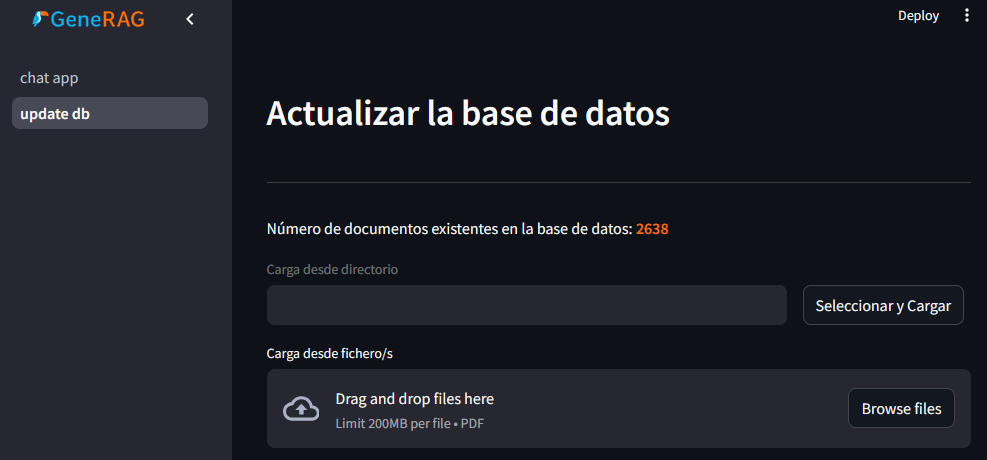
\includegraphics[width=.9\textwidth]{imagenes/0075_update2.png}
                \caption{Interfaz. Diseño de la página de carga y actualización de la base de datos}
                \label{fig:0075_update2}
            \end{figure}     

            \noindent En cuanto al código necesario para actualizar la base de datos, desarrollamos en la clase \textit{Chatbot} varias alternativas para incluir nuevos documentos. En la parte a) de la figura \ref{fig:0077_update_4} podemos ver la versión para cargar todos los documentos de un directorio, ya que usa la clase \textit{PyPDFDirectoryLoader} (la versión para cargar ficheros individuales es exactamente igual, salvo por la carga individual con \textit{PyPDFLoader}). También podemos observar como separa los documentos (\textit{text\_splitter}), genera diferentes IDs (\textit{\_\_calculate\_chunk\_ids}) y los incluye en la base de datos (\textit{vector\_store}).

            \noindent La parte b) de la misma figura muestra como se generan los IDs para los documentos, formándolos con partes de sus metadatos: nombre de archivo, número de página y número del fragmento en la página (depende del tamaño del chunk asignado, una página puede contener de 2 a 5 trozos). De esta forma obtenemos la referencia completa de donde ha obtenido la información el RAG ante una consulta de usuario (ver siguiente sección, figura \ref{fig:0096_interfaz5}).

            \begin{figure}[H]
                \centering
                \begin{subfigure}{0.49\textwidth}
                    \centering
                    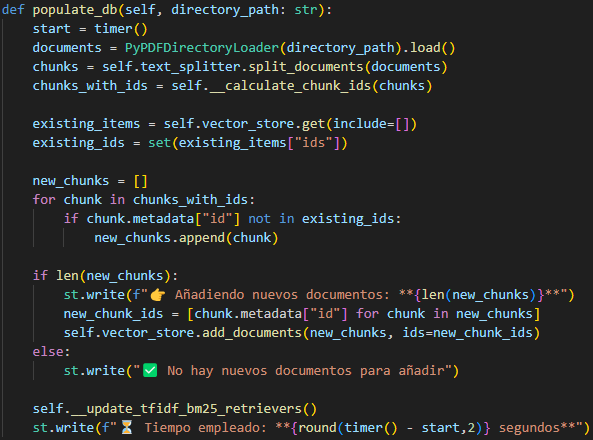
\includegraphics[width=1\textwidth]{imagenes/0076_update_3.png}
                    \caption{Método populate\_db}
                \end{subfigure}   
                \begin{subfigure}{0.49\textwidth}
                    \centering
                    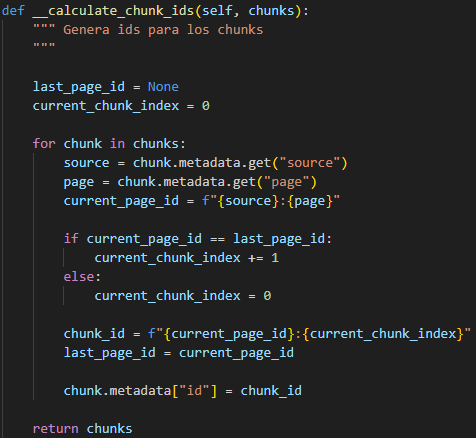
\includegraphics[width=1\textwidth]{imagenes/0077_update_4.png}
                    \caption{Método \_\_calculate\_chunk\_id}
                \end{subfigure}                  
                \caption{Clase Chatbot. Fragmentos de código de algunos de los métodos usados para actualizar la base de datos}
                \label{fig:0077_update_4}
            \end{figure}            

            \noindent El código de esta clase esta disponible en la carpeta \textit{classes} del repositorio \cite{0045_repo}, en el archivo \textbf{chatbot.py}. 

            \noindent Finalizaremos este apartado mostrando algunas figuras de los cuadros de diálogo diseñados al añadir archivos a nuestra base de datos.

            \begin{figure}[H]
                \centering
                
\includegraphics[width=.6\textwidth]{imagenes/0078_waiting.png}
                \caption{Interfaz. Cuadro de dialogo de tiempo de espera}		
                \label{fig:0078_waiting}
            \end{figure}

            \begin{figure}[H]
                \centering
                \begin{subfigure}{0.49\textwidth}
                    \centering
                    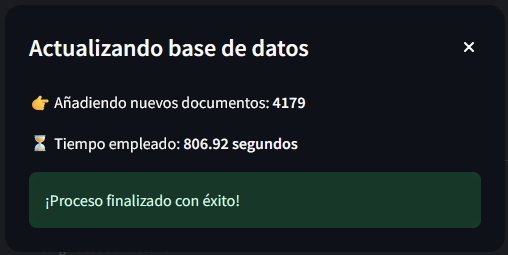
\includegraphics[width=1\textwidth]{imagenes/0079_nomic_512.png}
                    \caption{nomic-embed-text}
                \end{subfigure}   
                \begin{subfigure}{0.49\textwidth}
                    \centering
                    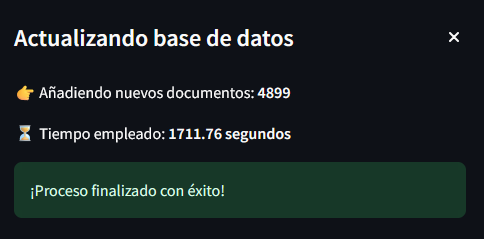
\includegraphics[width=1\textwidth]{imagenes/0079_bge_512.png}
                    \caption{bge-m3}
                \end{subfigure}    
                \begin{subfigure}{0.49\textwidth}
                    \centering
                    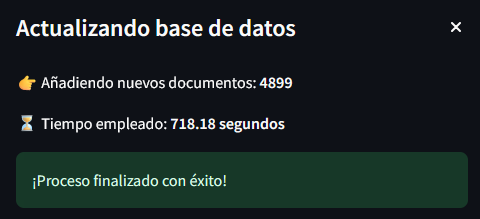
\includegraphics[width=1\textwidth]{imagenes/0079_jina_512.png}
                    \caption{jina-embeddings-v2-base-es}
                \end{subfigure}   
                \begin{subfigure}{0.49\textwidth}
                    \centering
                    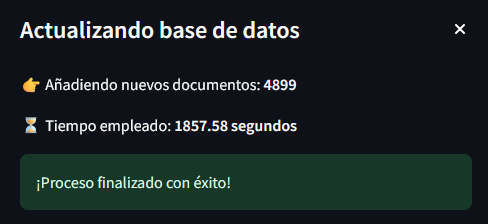
\includegraphics[width=1\textwidth]{imagenes/0079_snow_512.png}
                    \caption{snowflake-arctic-embed2}
                \end{subfigure}               
                \caption{Interfaz. Cuadros de dialogo. Tiempos para bases de datos con documentos de tamaño 512}
                \label{fig:0079_success1}
            \end{figure} 

            \begin{figure}[H]
                \centering
                \begin{subfigure}{0.49\textwidth}
                    \centering
                    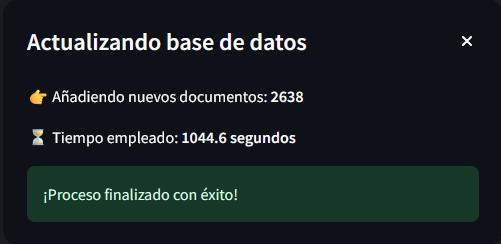
\includegraphics[width=1\textwidth]{imagenes/0079_nomic_1024.png}
                    \caption{nomic-embed-text}
                \end{subfigure}   
                \begin{subfigure}{0.49\textwidth}
                    \centering
                    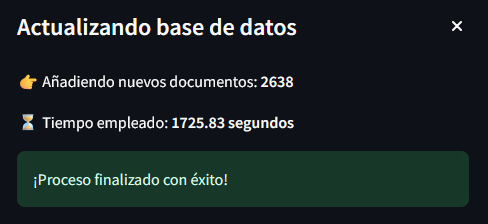
\includegraphics[width=1\textwidth]{imagenes/0079_bge_1024.png}
                    \caption{bge-m3}
                \end{subfigure}    
                \begin{subfigure}{0.49\textwidth}
                    \centering
                    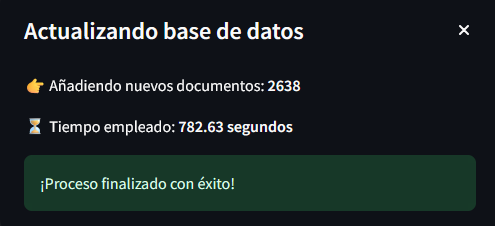
\includegraphics[width=1\textwidth]{imagenes/0079_jina_1024.png}
                    \caption{jina-embeddings-v2-base-es}
                \end{subfigure}   
                \begin{subfigure}{0.49\textwidth}
                    \centering
                    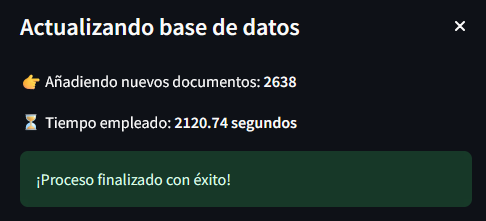
\includegraphics[width=1\textwidth]{imagenes/0079_snow_1024.png}
                    \caption{snowflake-arctic-embed2}
                \end{subfigure}               
                \caption{Interfaz. Cuadros de díalogo. Tiempos para bases de datos con documentos de tamaño 1024}
                \label{fig:0079_success2}
            \end{figure} 

            \noindent Si nos fijamos en las figuras \ref{fig:0079_success1} y \ref{fig:0079_success2}, destaca la diferencia de tiempo existente entre el par nomic-jina y bge-snowflake, siendo estos últimos los que más tiempo consumen al incluir nuevos documentos en la base de datos vectorial. El motivo para esta diferencia puede residir en una metodología más compleja para vectorizar los documentos de este último par, puesto que son los modelos más pesados en comparación.
            
            \noindent En contraste con los modelos locales, el tiempo de embedding del modelo \textit{text-embedding-3-small} (OpenAI) es extremadamente rápido. Como se puede observar en la figura \ref{fig:0099_te3s-embed}, el modelo vectoriza todos los documentos en solo 40 segundos.
            
            \begin{figure}[H]
            	\centering
            	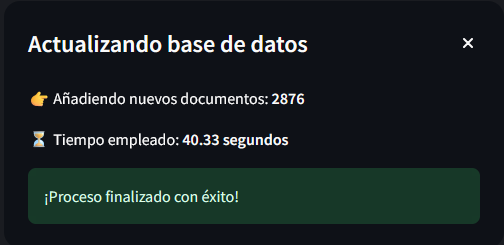
\includegraphics[width=.6\textwidth]{imagenes/0099_te3s-embed.png}
            	\caption{Interfaz. Tiempo de embedding de \textit{text-embedding-3-small}}		
            	\label{fig:0099_te3s-embed}
            \end{figure}

        \subsection{Interfaz del chatbot: Recuperación y generación de información}  
        \label{sec:interfaz_chatbot}

            En este apartado explicaremos el funcionamiento de la interfaz del chatbot del sistema RAG, mostrando los apartados correspondientes a la recuperación y generación de información especialmente. Ayudándonos de \textit{Streamlit}, se ha implementado página principal (figura \ref{fig:0080_interfaz_main}) con dos elementos personalizables: modelo de lenguaje y estrategia de búsqueda; y el chat.

            \begin{figure}[H]
                \centering
                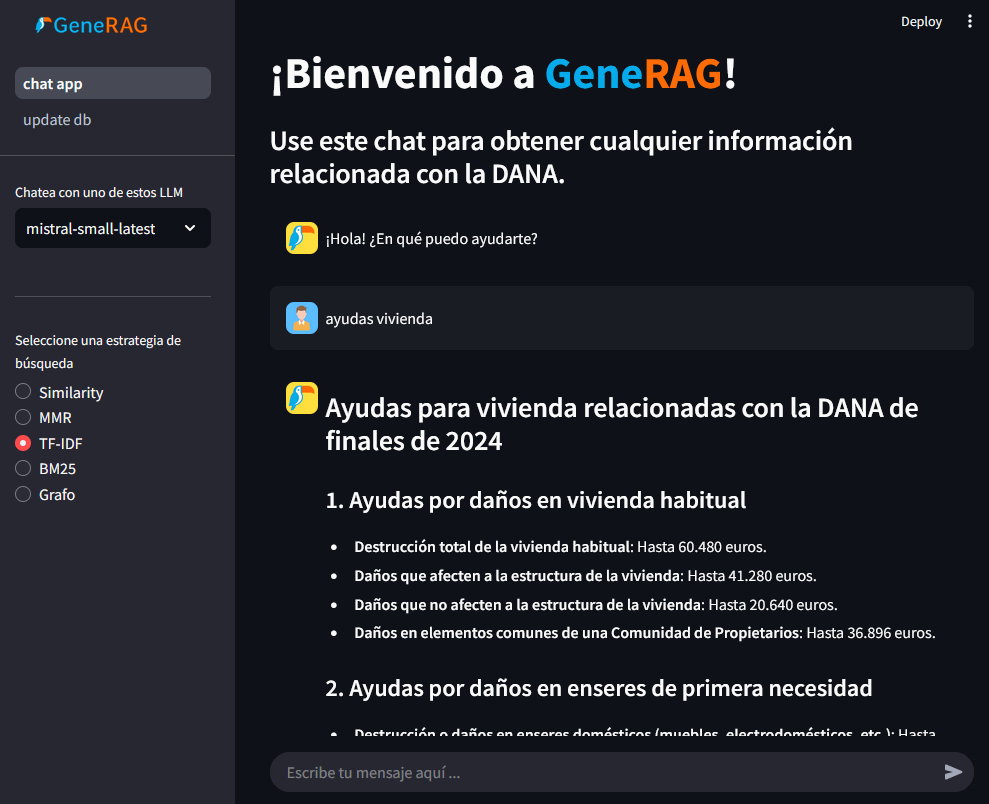
\includegraphics[width=1\textwidth]{imagenes/0080_interfaz_main.png}
                \caption{Interfaz. Página principal}		
                \label{fig:0080_interfaz_main}
            \end{figure}

            \noindent En la figura \ref{fig:0080_interfaz_main} se pueden observar los elementos los elementos mencionados en el párrafo anterior, situados en la barra lateral izquierda; ademas del chat con una conversación entre el usuario y el sistema RAG. A continuación, pasaremos a explicar el funcionamiento interno de estos elementos proporcionados por \textit{Streamlit} y también, las partes de recuperación y generación de información en la parte del chat.        

            \subsubsection{Configuración inicial del chatbot}

                \noindent Al igual que en la página de actualización de la base de datos (figura \ref{fig:0074_update1}), también necesitamos configurar el chatbot en la página principal.  
    
                \begin{figure}[H]
                    \centering
                    \begin{subfigure}{0.49\textwidth}
                        \centering
                        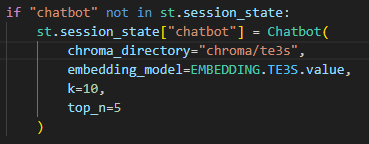
\includegraphics[width=1\textwidth]{imagenes/0081_chatbot.png}
                        \caption{Chatbot interfaz web}
                    \end{subfigure}   
                    \begin{subfigure}{0.49\textwidth}
                        \centering
                        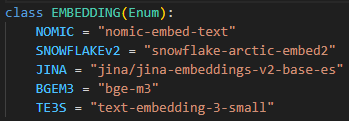
\includegraphics[width=1\textwidth]{imagenes/0081_embeddings.png}
                        \caption{Clase EMBEDDING}
                    \end{subfigure}                  
                    \caption{Fragmentos de código. Declaración de la variable Chatbot en la interfaz principal y clase EMBEDING}
                    \label{fig:0081_chatbot}
                \end{figure}   

                \noindent En la parte a de la figura anterior, se observan los detalles aportados para dicha configuración. Indicamos el modelo de embedding (del cual podemos elegir entre las opciones disponibles vistas en la parte b), los documentos recuperados (\textbf{k}) y los documentos filtrados por el reranker (\textbf{top\_n)}. Como se observa en la figura, este ejemplo usa el modelo de embedding \textit{text-embedding-3-small} junto un modelo de reranking, que se encargará de filtrar los cinco mejores documentos de los diez recuperados por el modelo de recuperación.

                \noindent La clase EMBEDDING esta situada en la carpeta \textit{classes}, en el fichero \textbf{LLM.py}. Los modelos de embedding disponibles deben ser descargados con antelación mediante Ollama (sección \ref{sec:ollama}) a excepción del modelo \textit{text-embedding-3-small}, del cual necesitaremos aportar nuestra clave de OpenAI.

            \subsubsection{Elementos de selección: selectbox y radio}  

                \textit{Streamlit} ofrece en su documentación oficial multitud de componentes que podemos usar en la interfaz web. Como se observó en la figura \ref{fig:0080_interfaz_main}, hemos usado una caja de selección (\textit{selectbox}) para elegir el modelo de lenguaje con el que chatear, y botones de radio (\textit{radio}) para escoger la estrategia de búsqueda del modelo de recuperación.

                \noindent El código mostrado en la parte a de la figura \ref{fig:0082_llms}, muestra la implementación de la caja de selección. La etiqueta \textit{sidebar} indica a Streamlit, que debe estar situado en la barra lateral, normalmente situada a la izquierda.

                \noindent De entre los parámetros, destacan: 

                \begin{itemize}
                    \item \textbf{options:} Lista de elementos que muestra la caja de selección (parte b, figura \ref{fig:0082_llms}).
                    \item \textbf{key:} Variable de \textit{session\_state} que tomará el valor determinado en la caja de selección.
                    \item \textbf{on\_change:} Función que se activará cuando cambie el valor de la caja de selección.
                \end{itemize}
    
                \begin{figure}[H]
                    \centering
                    \begin{subfigure}{0.49\textwidth}
                        \centering
                        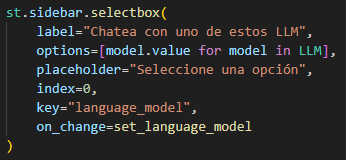
\includegraphics[width=1\textwidth]{imagenes/0082_selectbox.png}
                        \caption{Selectbox LLMs}
                    \end{subfigure}   
                    \begin{subfigure}{0.49\textwidth}
                        \centering
                        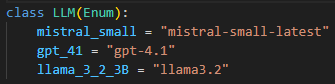
\includegraphics[width=1\textwidth]{imagenes/0082_llms.png}
                        \caption{Clase LLM}
                    \end{subfigure}                  
                    \caption{Fragmentos de código. Caja de selección de los modelos de lenguaje y clase LLM.}
                    \label{fig:0082_llms}
                \end{figure}        

                \noindent Los modelos disponibles vistos en la parte b de la figura \ref{fig:0082_llms}, han de ser descargados usando \textit{Ollama}; exceptuando los modelos de \textit{Mistral AI} y de \textit{OpenAI}, del cual necesitamos un código de su API.

                \noindent La función \textit{set\_language\_model} (figura \ref{fig:083_set_llm}) usa un método disponible en la clase Chatbot que cambia el modelo de lenguaje a usar por el RAG (figura \ref{fig:084_set_llm2}). Dicho método actua diferente según el modelo elegido, necesitando la clave API para los modelos de \textit{Mistral AI} y \textit{OpenAI}. El método es similar al aportado en el constructor, figura \ref{fig:0069_chatbot_const_2}.
    
                \begin{figure}[H]
                    \centering
                    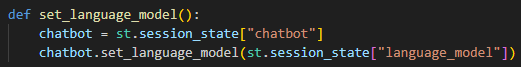
\includegraphics[width=.8\textwidth]{imagenes/083_set_llm.png}
                    \caption{Función de la interfaz. Modificar el modelo de lenguaje}		
                    \label{fig:083_set_llm}
                \end{figure}
    
                \begin{figure}[H]
                    \centering
                    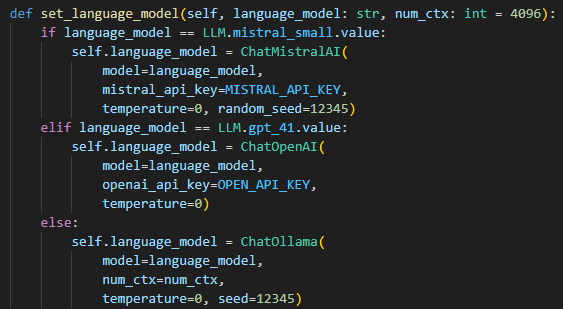
\includegraphics[width=.8\textwidth]{imagenes/084_set_llm2.png}
                    \caption{Clase Chatbot. Modificar el modelo de lenguaje}		
                    \label{fig:084_set_llm2}
                \end{figure}   

                \noindent La selección en radio, se implementa de forma similar (parte a de la figura \ref{fig:0084_radio}). Los valores entre los que seleccionar, en este caso han de ser aportados entre corchetes. Entre los demás parámetros destacan:

                \begin{itemize}
                    \item \textbf{key:} Variable de \textit{session\_state} que tomará el valor determinado en la selección de radio.
                    \item \textbf{on\_change:} Función que se activa al cambiar el valor de la selección de radio.
                \end{itemize}

                \noindent La función de la interfaz vista en la parte b de la figura \ref{fig:0084_radio}, activa el método de clase Chatbot para cambiar la estrategia de búsqueda. 
    
                \begin{figure}[H]
                    \centering
                    \begin{subfigure}{0.49\textwidth}
                        \centering
                        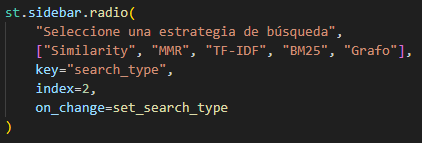
\includegraphics[width=1\textwidth]{imagenes/0084_radio_1.png}
                        \caption{Selección de radio, estrategias de búsqueda}
                    \end{subfigure}   
                    \begin{subfigure}{0.49\textwidth}
                        \centering
                        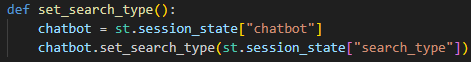
\includegraphics[width=1\textwidth]{imagenes/0084_radio_2.png}
                        \caption{Función de la interfaz}
                    \end{subfigure}                  
                    \caption{Fragmentos de código. Selección de radio para las estrategias de búsqueda y función de la interfaz para cambiarlas}
                    \label{fig:0084_radio}
                \end{figure}        
    
                \noindent Como se observa en la figura siguiente, cada estrategia cambia el método de recuperación (\textit{retriever}). Las estrategias \textit{similarity} y \textit{mmr} son traidas por defecto en la base de datos Chroma, mientras que para las demás tenemos que usar clases externas: \textit{TFIDFRetriever}, \textit{BM25Retriever} y \textit{GraphRetriever}. (El método es similar al aportado en el constructor, figura \ref{fig:0071_chatbot_const_4}).
    
                \begin{figure}[H]
                    \centering
                    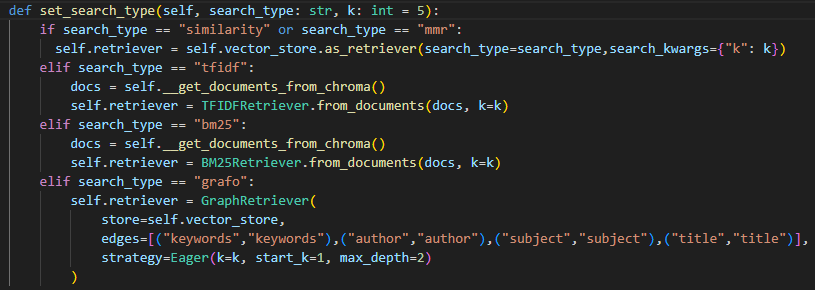
\includegraphics[width=.9\textwidth]{imagenes/0085_radio_3.png}
                    \caption{Clase Chatbot. Modificar la estrategia de búsqueda}		
                    \label{fig:0085_radio_3}
                \end{figure}            

            \subsubsection{Recuperación y generación de información}

                La parte dedicada a la interfaz del chatbot consta de varios bloques diferenciados, como se puede observar en la figura \ref{fig:0086_chat_codigo}. 
                
                \noindent En las primeras dos líneas (85-86) se crea la variable \textit{chat\_history} si no se encuentra disponible en la variable de sesión \textit{session\_state}, y le agrega un mensaje del sistema dando la bienvenida al chat. En dicha variable iremos guardando todo el historial de conversación entre el usuario y el sistema.

                \noindent El bucle for de las líneas 88 a 94 recorre cada mensaje disponible en la variable de sesión \textit{chat\_history}. Cada mensaje es diferenciado entre sistema y usuario (\textit{AIMessage} y \textit{HumanMessage}), y son impresos con distintos avatares según corresponda.

                \noindent La variable \textit{user\_query} de la línea 96, guarda la consulta hecha por el usuario. Esta consulta es retornada gracias al elemento de \textit{Streamlit} \textit{chat\_input}, que genera una entrada de texto flotante en la interfaz y en la que se puede escribir.

                \noindent A continuación, dicha entrada de texto se agrega al historial de conversación marcada como mensaje de usuario (\textit{HumanMessage}). Genera la respuesta del sistema llamando a la función \textit{query} (que explicaremos seguidamente), y agrega la respuesta al historial de conversación como \textit{AIMessage}. 
    
                \begin{figure}[H]
                    \centering
                    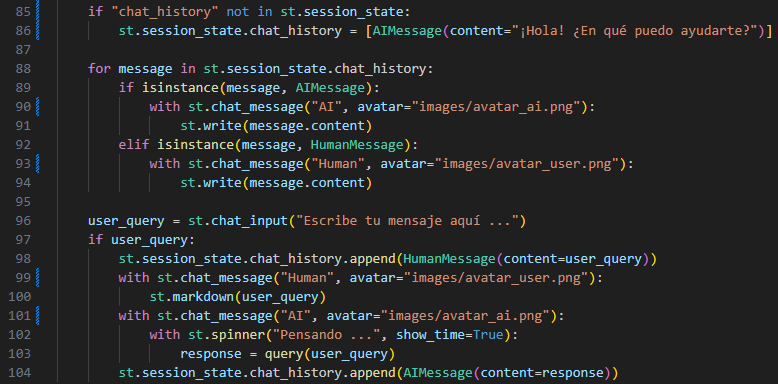
\includegraphics[width=.9\textwidth]{imagenes/0086_chat_codigo.png}
                    \caption{Fragmento de código correspondiente a la interfaz del chatbot}		
                    \label{fig:0086_chat_codigo}
                \end{figure}

                \noindent En la función \textit{query} vista en la figura \ref{fig:0087_chat_query}, suceden ambos procesos de recuperación y generación de información. La recuperación se da entre las líneas 20 a la 23, y la generación en la 42; pero entre ellas se producen otros procesos que dan más detalle y riqueza a la respuesta, y que pasaremos a explicar con detenimiento.

                \noindent En las líneas 20 y 21 se consigue el modelo de recuperación (\textit{retriever}) usado por el \textit{chatbot}. En el ejemplo se usa un modelo de recuperación con un reranker, el cuál efectuará un doble filtrado de los documentos recuperados por el modelo principal. 
                
                \noindent El método para iniciar la recuperación se ve en la línea 23. Mediante \textit{invoke}, el \textit{retriever} seleccionará los documentos más relevantes a la consulta proporcionada por el usuario a través del parámetro \textit{question}.

                \noindent A continuación, guardamos el contexto recuperado por el modelo (línea 84), es decir, el contenido del texto de los documentos recuperados. También guardamos ciertos metadatos (línea 25-39) de los documentos. En el ejemplo, usamos el ID del documento para mostrarlo junto con la respuesta del sistema, ofreciendo así un extra de información y referencias al usuario de donde ha sido obtenida la información.

                \noindent Para finalizar con la figura \ref{fig:0087_chat_query}, queda explicar la generación de información. Se encuentra en la línea 42, realizandose mediante la llamada al método de la clase \textit{Chatbot} \textit{answer\_query} y aportando sólo dos parámetros: la pregunta (\textit{question}) y el contexto (\textit{context}). La respuesta se guarda en la variable \textit{response\_text} mediante la función \textit{write\_stream} provista por Streamlit, que genera una escritura en tiempo real (\textit{token} a \textit{token}).

                \noindent Las variables \textit{response\_text} y \textit{sources} son retornadas por esta función, que terminarán siendo agregadas al historial de conversación.
    
                \begin{figure}[H]
                    \centering
                    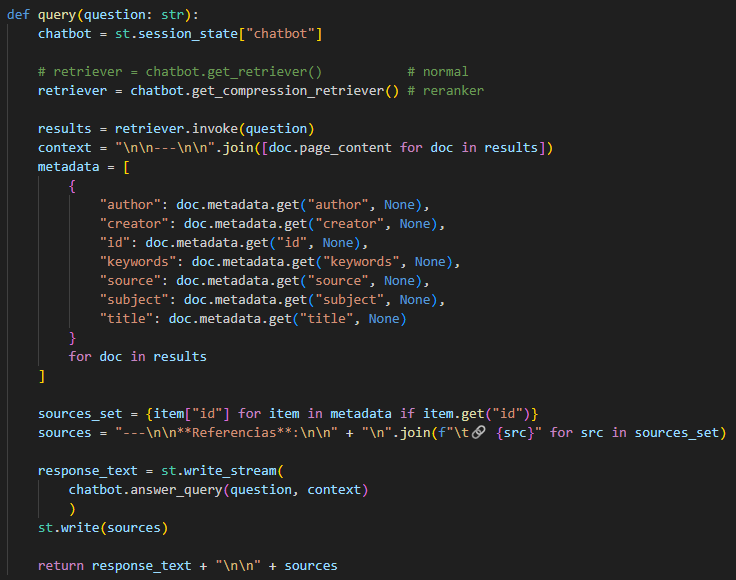
\includegraphics[width=.9\textwidth]{imagenes/0087_chat_query.png}
                    \caption{Función \textit{query} de la interfaz del chatbot. Hace los procesos de recuperación y generación de información del sistema RAG}		
                    \label{fig:0087_chat_query}
                \end{figure}

                \noindent La figura \ref{fig:0088_chat_answer} muestra el funcionamiento del método \textit{answer\_query} de la clase \textit{Chatbot}. En la figura podemos observar el funcionamiento de la cadena (\textit{query\_chain}) que nos brinda \textit{LangChain} para trabajar con modelos de lenguaje. En esta cadena podemos combinar el modelo de recuperación, los parámetros necesarios para el \textit{prompt}, la propia plantilla del prompt y el modelo de lenguaje. Generando así, la respuesta de forma más simple y eficiente con el comando \textit{stream}, que al igual que antes, genera la respuesta en tiempo real (\textit{token} a \textit{token}).
    
                \begin{figure}[H]
                    \centering
                    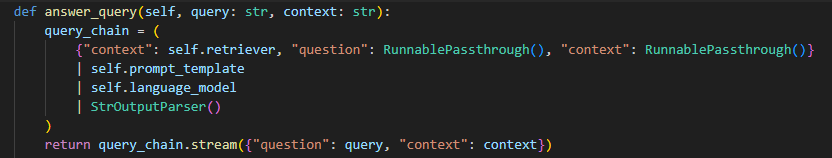
\includegraphics[width=.9\textwidth]{imagenes/0088_chat_answer.png}
                    \caption{Método \textit{answer\_query} de la clase Chatbot, retorna la respuesta del sistema RAG}		
                    \label{fig:0088_chat_answer}
                \end{figure}  

                \noindent Para finalizar este apartado, solo queda mostrar el \textit{prompt} usado por defecto por el \textit{chatbot}. La figura \ref{fig:0089_def_prompt} muestra la plantilla aplicada, en el ella se hace énfasis en el detalle y organización que deben presentar las respuestas. También se observan en las últimas dos líneas, como han de aportarse los argumentos con los que debe generar la respuesta: la pregunta y el contexto. 

                \noindent El planteamiento, instrucciones u órdenes escritas en el prompt, pueden generar distintas respuestas por el modelo de lenguaje. Por lo tanto, hay que buscar la forma adecuada para que el modelo de lenguaje obtenga mejores resultados.
    
                \begin{figure}[H]
                    \centering
                    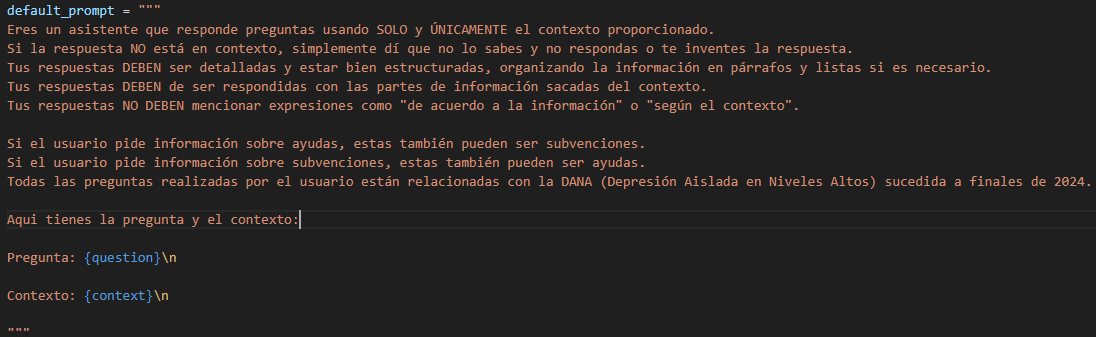
\includegraphics[width=1\textwidth]{imagenes/0089_def_prompt.png}
                    \caption{Prompt por defecto usado en el proyecto}		
                    \label{fig:0089_def_prompt}
                \end{figure}     

            \subsubsection{Capturas del chatbot}                   
    
                \begin{figure}[H]
                    \centering
                    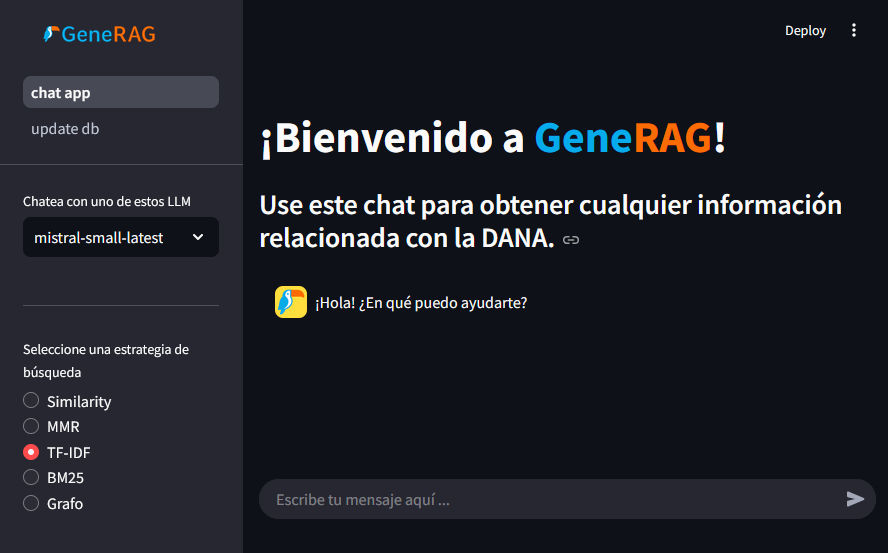
\includegraphics[width=.9\textwidth]{imagenes/0092_interfaz1.png}
                    \caption{Interfaz web del chatbot}		
                    \label{fig:0092_interfaz1}
                \end{figure}                   
    
                \begin{figure}[H]
                    \centering
                    
\includegraphics[width=.9\textwidth]{imagenes/0093_interfaz2.png}
                    \caption{Interfaz web con la barra lateral izquierda plegada}		
                    \label{fig:0093_interfaz2}
                \end{figure}                   
    
                \begin{figure}[H]
                    \centering
                    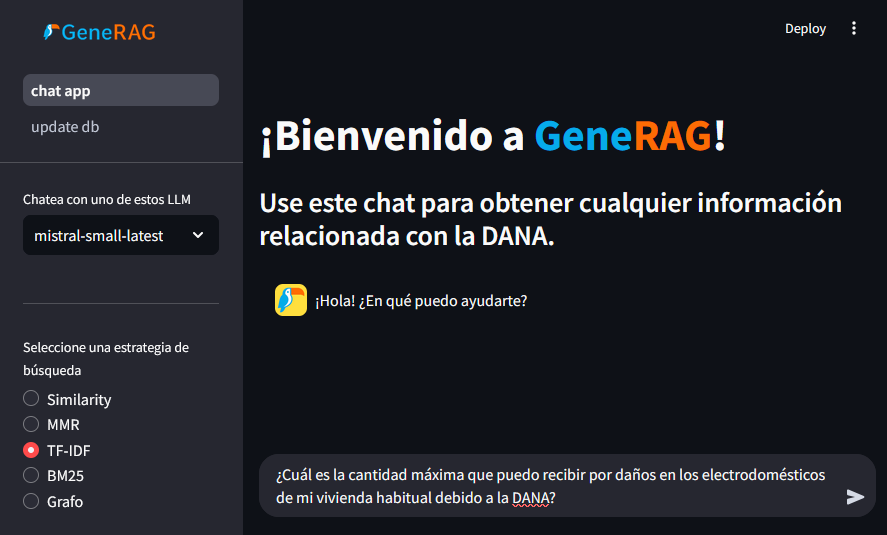
\includegraphics[width=.9\textwidth]{imagenes/0094_interfaz3.png}
                    \caption{Interfaz web con pregunta}		
                    \label{fig:0094_interfaz3}
                \end{figure}                   
    
                \begin{figure}[H]
                    \centering
                    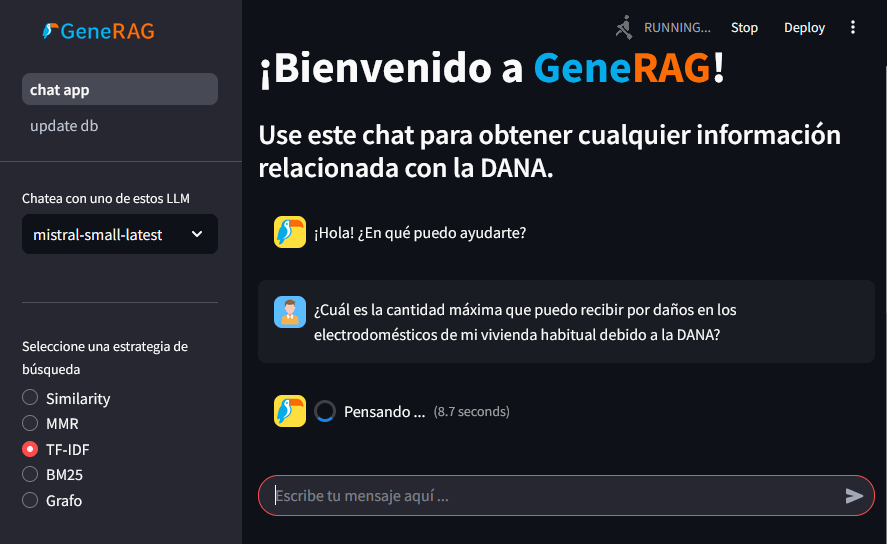
\includegraphics[width=.9\textwidth]{imagenes/0095_interfaz4.png}
                    \caption{Interfaz web generando respuesta}		
                    \label{fig:0095_interfaz4}
                \end{figure}                   
    
                \begin{figure}[H]
                    \centering
                    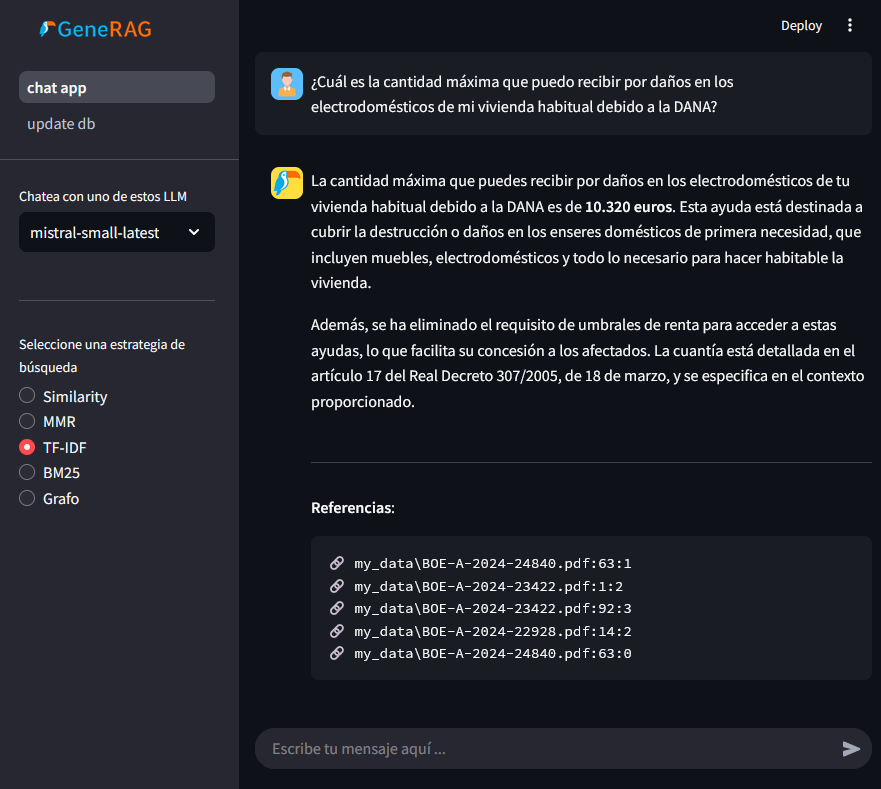
\includegraphics[width=.9\textwidth]{imagenes/0096_interfaz5.png}
                    \caption{Interfaz web con respuesta generada y referencias}		
                    \label{fig:0096_interfaz5}
                \end{figure}     
                
	\section{Conclusiones sobre el desarrollo de la aplicación}			
	
		El desarrollo de este proyecto ha puesto de manifiesto las claras ventajas de adoptar un enfoque basado en \textbf{RAG} frente a la solución planteada inicialmente: RASA. Como hemos comentado, RASA depende de un sistema de \textit{intents} y respuestas predefinidas, que exige un mantenimiento continuo y una anticipación de escenarios de interacción; el modelo con RAG ofrece una mayor versatilidad. Gracias a la integración continua con \textit{GitHub Actions}, la base de conocimiento se actualiza automáticamente con los documentos del BOE, lo que garantiza sincronización con la fuente original y reduce de forma significativa las tareas de mantenimiento.
		
		\noindent La incorporación de \textit{LangChain} resultó clave en la integración de los distintos componentes, facilitando las tareas de recuperación y generación de información. El proceso de desarrollo estuvo además favorecido por la abundante documentación y los numerosos tutoriales disponibles, lo que permitió una rápida implementación y conexión con diferentes plataformas de modelos de lenguaje.
		
		\noindent Por su parte, la interfaz desarrollada con \textit{Streamlit} ofreció una experiencia moderna y práctica. Su capacidad de generar aplicaciones web inyectando código \textit{Python} simplificó el trabajo, al permitir el uso de elementos interactivos habituales sin necesidad de programación adicional desde el \textit{backend}. De esta manera, se aceleró la construcción de la interfaz, la personalización y la adaptación del sistema a las necesidades específicas del proyecto.
		
		\noindent En conjunto, el nuevo enfoque proporciona un sistema más preciso, rápido y escalable. Así, se superan las limitaciones del marco anterior y se establece una solución sólida, eficiente y preparada para su evolución futura.

\endgroup


\begingroup
\titleformat{\chapter}[block]
{\normalfont\Huge\bfseries\centering} 
{Capítulo \thechapter} 
{0.5em}
{: \LARGE}
[\vspace{1em}\titlerule]

\titlespacing*{\chapter}{0pt}{-60pt}{40pt}

\chapter{Evaluación del Proyecto}
\label{cap:4_results}

	En este capítulo se describen los procesos realizados para evaluar nuestro sistema RAG. Para ello se ha generado un conjunto de preguntas junto a varios agentes críticos, sobre los que se evalúa la generación de respuesta de los modelos de lenguaje elegidos en el proyecto (ver sección \ref{sec:cap2_llms_usados}). El objetivo de realizar estas pruebas es mostrar el rendimiento de diferentes modelos de lenguaje sobre un mismo dataset de preguntas.
	
	\noindent En las siguientes secciones explicamos como se ha generado el conjunto de preguntas y como se han definido los agentes críticos para evaluar el RAG. También mostramos los resultados obtenidos, razonando el porqué de ellos. 
	
	\noindent Y para finalizar el capítulo, se elaboran posibles casos de uso para nuestro sistema RAG y respondemos algunas preguntas relacionadas con el impacto causado al cambiar ciertos parámetros de un sistema RAG.
	
	\section{Generación del conjunto de preguntas}	
	\label{sec:4_gen_dataset}
	
		En la creación del conjunto de preguntas, hemos optado por usar el modelo de lenguaje \textit{mistral-small} para generar preguntas basadas en nuestra fuente de conocimiento (documentos PDF del Boletín Oficial del Estado relacionados con la DANA).
		
		\noindent En la siguiente figura, vemos la configuración del modelo de lenguaje \textit{mistral-small} que hemos usado. Al ser un modelo externo, necesitamos aportar su clave de acceso. Si nos fijamos en la figura \ref{fig:0100_eval_gen_1}, le hemos indicado que sea un poco creativo en la generación del par pregunta-respuesta aumentando el parámetro de \textit{temperature}. 
	
		\begin{figure}[H]
			\centering
			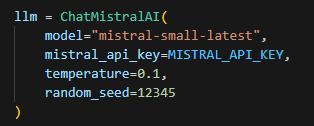
\includegraphics[width=.4\textwidth]{imagenes/0100_eval_gen_1.png}
			\caption{Configuración LLM de generación del conjunto de preguntas}		
			\label{fig:0100_eval_gen_1}
		\end{figure} 
		
		\noindent El siguiente paso en la generación del conjunto de preguntas es facilitar al modelo de lenguaje las instrucciones necesarias mediante un \textit{prompt} para generar el conjunto de preguntas. 
		
		\noindent Fijándose en la figura \ref{fig:0101_eval_gen_2}, el prompt hace especial hincapié en la necesidad del usuario de generar una única pregunta con su respuesta, siempre estando relacionado con la DANA y dado un determinado contexto. La pregunta debe mantener un formato muy específico y la salida debe presentarse separado por comas (para su posterior procesado en formato csv).
		
		\noindent El contexto aportado al final del prompt se refiere al contenido en texto de cada página de cada documento presente en la fuente de conocimiento, por lo que es necesario ejecutar el prompt varias veces en bucle. El número de ficheros que integraban dicha fuente en el momento de la generación de este conjunto de preguntas y respuestas era de alrededor de 80 con un total de más de 560 páginas.
		
		\begin{figure}[H]
			\centering
			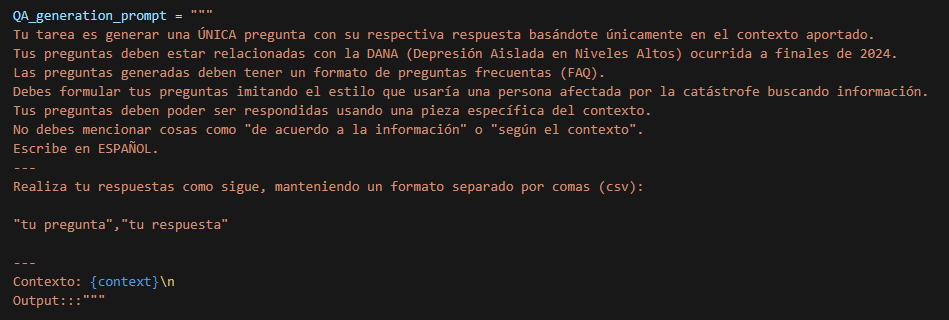
\includegraphics[width=1\textwidth]{imagenes/0101_eval_gen_2.png}
			\caption{Prompt usado en la generación del conjunto de preguntas}		
			\label{fig:0101_eval_gen_2}
		\end{figure} 
		
		\noindent Para añadir los documentos hemos vuelto a usar la clase \textit{PyPDFDirectoryLoader}, pasando como argumento la carpeta donde hemos descargado con anterioridad los ficheros de nuestra fuente de conocimiento. La figura \ref{fig:0103_eval_gen4} muestra este proceso y el de configuración inicial de la cadena \textit{chain}, siendo similar a lo mostrado con anterioridad en otros apartados.
		
		\begin{figure}[H]
			\centering
			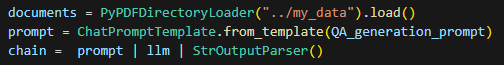
\includegraphics[width=0.6\textwidth]{imagenes/0103_eval_gen4.png}
			\caption{Carga de datos y preparación del modelo de lenguaje}		
			\label{fig:0103_eval_gen4}
		\end{figure} 
		
		\noindent El bucle antes mencionado, en el cual se deben generar todas las preguntas se puede apreciar en la figura \ref{fig:0102_eval_gen_3}. En dicha figura, se crea un fichero para albergar el conjunto entero de preguntas-respuestas, donde cada línea del fichero contendrá:
		
		\begin{itemize}
			\item \textbf{Pregunta:} La pregunta generada por el modelo de lenguaje.
			\item \textbf{Respuesta:} La respuesta a la pregunta generada por el modelo de lenguaje.
			\item \textbf{Contexto:} El contexto del cual se ha generado la pregunta.
			\item \textbf{Recurso:} El fichero del cual se ha conseguido el contexto.
		\end{itemize}
		
		\begin{figure}[H]
			\centering
			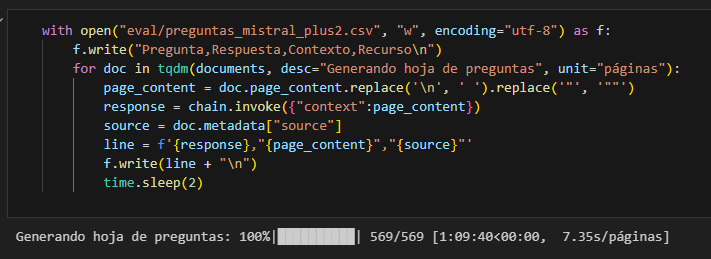
\includegraphics[width=0.8\textwidth]{imagenes/0102_eval_gen_3.png}
			\caption{Bucle para la generación del conjunto de preguntas}		
			\label{fig:0102_eval_gen_3}
		\end{figure} 
		
		\noindent La generación de este conjunto de preguntas ha tenido una duración en tiempo de una hora y diez minutos aproximadamente. La inclusión en el bucle de la parada (\textit{time.sleep(2)}) de dos segundos fue necesario para evitar el error por sobrecarga  del modelo (recordemos que es un modelo externo ofrecido de forma gratuita por \textit{Mistral AI}). Sin esta parada, la duración habría sido de alrededor de unos cincuenta minutos.
		
		\noindent El resultado final de la ejecución esta disponible en el recurso \cite{0042_pregu} de la bibliografía. El número final de preguntas se redujo a 300 debido a que existía bastante repetición entre las preguntas generadas. Una muestra de las quince primeras líneas de este fichero pueden observarse en la siguiente figura.
		
		\begin{figure}[H]
			\centering
			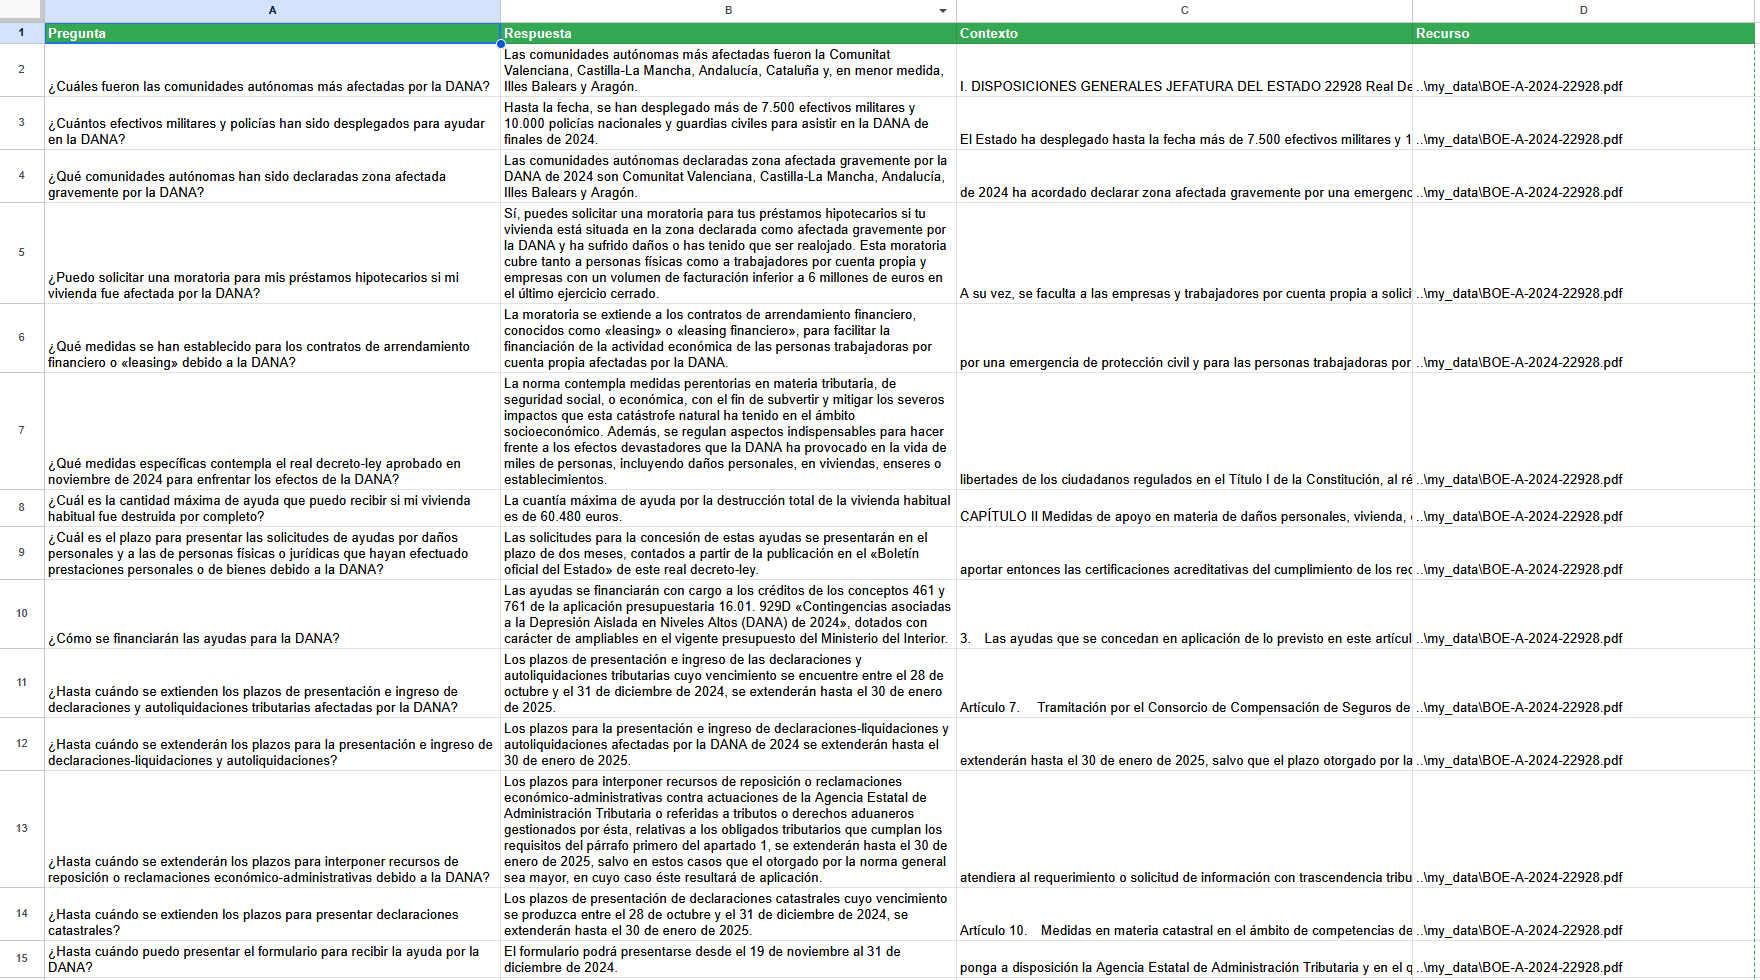
\includegraphics[width=1\textwidth]{imagenes/0103_eval_gen_4.png}
			\caption{Muestra del conjunto de preguntas \cite{0042_pregu}}		
			\label{fig:0103_eval_gen_4}
		\end{figure} 
		
		\noindent \textbf{Nota:} El fichero de generación de preguntas esta disponible en la raíz del proyecto \cite{0045_repo}, bajo el nombre \textbf{qa\_generator.ipynb} (formato Jupyter Notebook).
		
	\section{Configuración de las alternativas de evaluación}
	
		En este apartado veremos la parte que precede al segundo objetivo de este Trabajo de Fin de Máster, donde mostraremos la configuración de las opciones utilizadas para las pruebas del sistema RAG. Empezaremos hablando de los modelos usados para dichas pruebas, los cuales se encargarán tanto de generar las respuestas como de evaluarlas.
		
		\noindent \textbf{Nota:} El código de las siguientes figuras se puede encontrar en el fichero \textbf{rag\_eval.ipynb} del repositorio \cite{0045_repo}.
				
		\subsection{Modelos evaluadores y configuración inicial}
		
			Como ya hemos comentado en la última sección del capítulo \ref{2_metods_eva}, se harán estas pruebas en tres modelos: el modelo gratuito y local \textit{llama3.2}, el modelo gratuito pero externo \textit{mistral-small} y el modelo externo y de pago \textit{gpt-4.1}. La siguiente figura muestra tres imágenes de la configuración de cada uno de estos modelos usando \textit{LangChain}. Como es común para los modelos externos, debemos proporcionar su clave API para poder usarlos.
		
			\begin{figure}[H]
				\centering
				\begin{subfigure}{.32\textwidth}
					\centering
					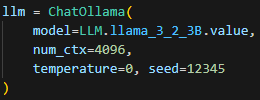
\includegraphics[width=1\textwidth]{imagenes/0106_eval_result3.png}
					\caption{Llama 3.2}
				\end{subfigure}   
				\begin{subfigure}{.32\textwidth}
					\centering
					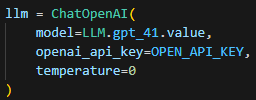
\includegraphics[width=1\textwidth]{imagenes/0105_eval_result2.png}
					\caption{GPT-4.1}
				\end{subfigure}        
				\begin{subfigure}{.32\textwidth}
					\centering
					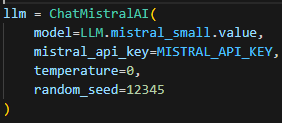
\includegraphics[width=1\textwidth]{imagenes/0104_eval_result1.png}
					\caption{Mistral Small 3.2}
				\end{subfigure}               
				\caption{Configuración de los modelos de lenguaje de pruebas}
				\label{fig:0106_eval_llms}
			\end{figure}  
			
			\noindent La variable \textit{model} común para todas las configuraciones de la figura anterior, contiene elementos de la clase \textit{LLM}. Estos elementos se corresponden con los nombres reales de los modelos que son usados para su acceso en la API y ya han sido mostrados en la figura \ref{fig:0082_llms}.
			
			\noindent El siguiente paso es configurar las demás variables de pruebas, la siguiente figura muestra alguna de ellas. En la primera línea podemos observar las estrategias de búsqueda que se probarán como mencionábamos en uno de los apartados de la sección \ref{2_metods_eva}. También observamos en la figura un \textit{prompt} que usaremos para medir la influencia en los resultados de un cambio en las instrucciones, en este caso más simples.
			
			\begin{figure}[H]
				\centering
				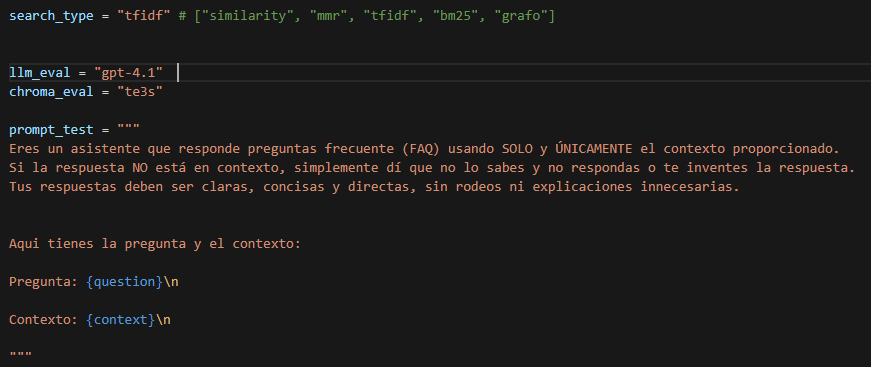
\includegraphics[width=.9\textwidth]{imagenes/0107_eval_result4.png}
				\caption{Variables de pruebas}		
				\label{fig:0107_eval_result4}
			\end{figure} 
			
			\noindent Las pruebas las realizaremos con dos \textit{chatbots}, la figura \ref{fig:0109_eval_result6} muestra la configuración de ambos. Los dos son exactamente iguales siendo el único cambio, el \textit{reranker} usado en el segundo de ellos (parte b). El caso de esta figura muestra una configuración de pruebas para modelos de \textit{OpenAI}, como se puede observar tanto por el modelo de lenguaje usado (\textit{gpt-4.1}) como por el de embedding (\textit{text-embedding-3-small}).
			
			\noindent Los modelos de embedding que probaremos están incluidos en la clase \textit{EMBEDDING} (ya mostrada en la figura \ref{fig:0081_chatbot}). El objetivo de la prueba de distintos modelos de embedding es dilucidar cual proporciona mejores resultados en la recuperación en conjunto con la generación de los modelos de lenguaje.
			
			\noindent \textbf{Nota:} Las clases \textit{LLM} y \textit{EMBEDDING} se encuentran en la carpeta \textit{classes} del repositorio \cite{0045_repo}.		 
			
			\begin{figure}[H]
				\centering
				\begin{subfigure}{.49\textwidth}
					\centering
					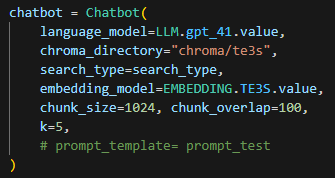
\includegraphics[width=1\textwidth]{imagenes/0108_eval_result5.png}
					\caption{Normal}
				\end{subfigure}   
				\begin{subfigure}{.49\textwidth}
					\centering
					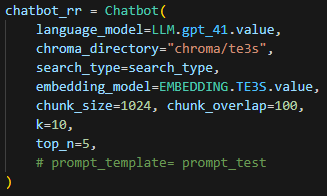
\includegraphics[width=1\textwidth]{imagenes/0109_eval_result6.png}
					\caption{Con reranker}
				\end{subfigure} 			
				\caption{Configuración de los chatbots de pruebas}
				\label{fig:0109_eval_result6}       
			\end{figure} 	
			
		\subsection{Agentes críticos}		
		
			Los agentes críticos son los encargados de realizar una evaluación de las respuestas generadas por los modelos de lenguaje. Las siguientes figuras muestran los \textit{prompts} con las instrucciones de los cuatro agentes críticos seleccionados para nuestras evaluaciones, y que están definidos en la sección \ref{2_metods_eva}.				
			
			\noindent El primero de ellos es el \textit{accuracy} (figura \ref{fig:0110_eval_result_agent1}), que es el encargado de evaluar la precisión de la respuesta generada por el modelo comparándola con la respuesta original. La figura muestra el \textit{prompt} con las instrucciones necesarias para que el modelo haga de evaluador comparando dos argumentos, e incluso, añadimos los criterios que tiene que seguir para asignar una nota.
			
			\noindent Todos los agentes evalúan de cero a cinco, siendo cero la peor nota y cinco la mejor.
			
			\begin{figure}[H]
				\centering
				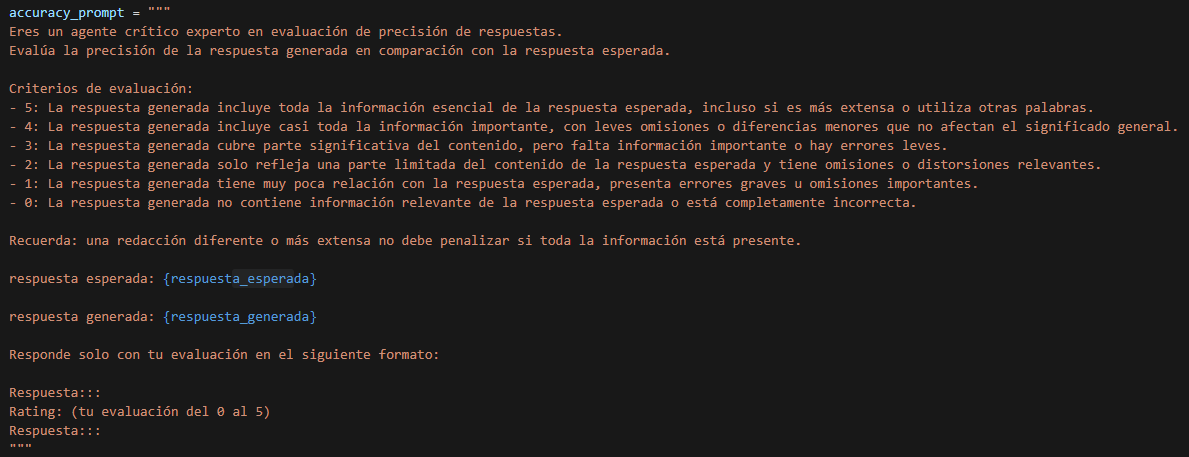
\includegraphics[width=1\textwidth]{imagenes/0110_eval_result_agent1.png}
				\caption{Agente crítico del accuracy}		
				\label{fig:0110_eval_result_agent1}
			\end{figure} 		
			
			\noindent El siguiente agente mide el \textit{faithfulness} (figura \ref{fig:0111_eval_result_agent2}). Esta medida evalúa el grado en que una respuesta esta basada en la información contenida en los documentos recuperados, por eso recibe estos dos argumentos. Gracias a esta medición obtenemos la fidelidad de la respuesta con los documentos de nuestra base de conocimiento.
			
			\begin{figure}[H]
				\centering
				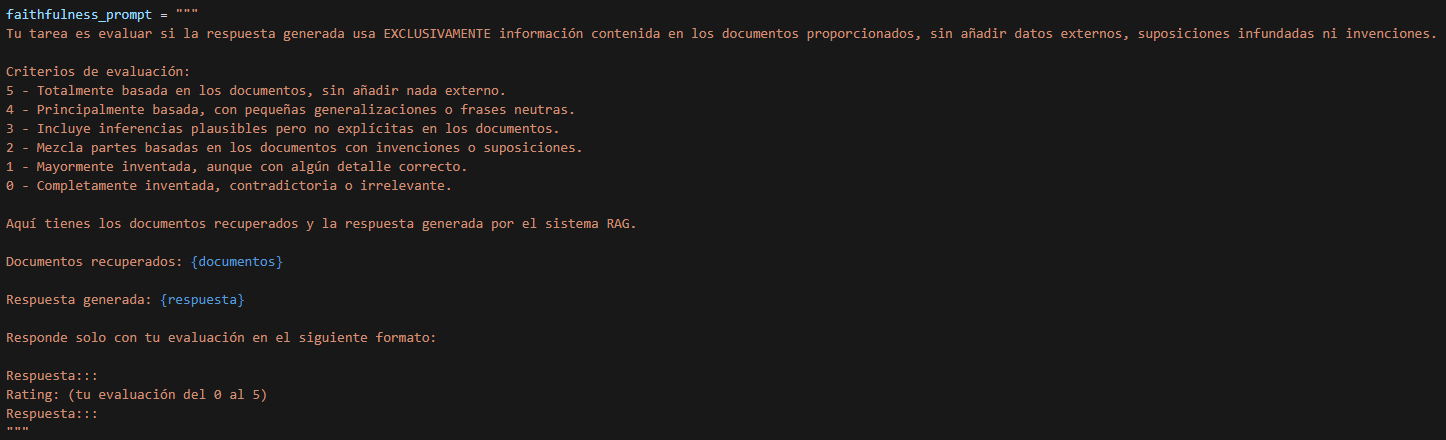
\includegraphics[width=1\textwidth]{imagenes/0111_eval_result_agent2.png}
				\caption{Agente crítico del faithfulness}		
				\label{fig:0111_eval_result_agent2}
			\end{figure} 	
			
			\noindent El \textit{groundedness} es una medida similar a la anterior (figura \ref{fig:0112_eval_result_agent3}), esta valora el uso de las evidencias aportadas por los documentos recuperados en la respuesta generada por el modelo. Es importante para mostrar lo bien (o mal) que usan la información disponible en los documentos recuperados a la hora de generar la respuesta.
			
			\begin{figure}[H]
				\centering
				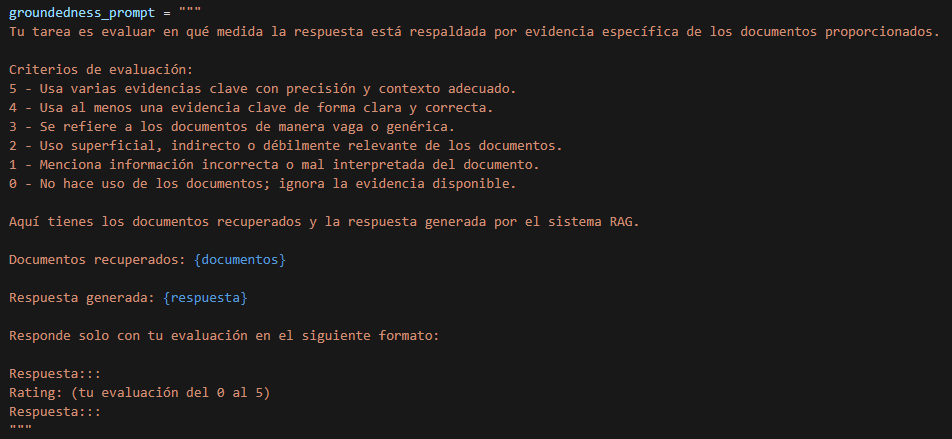
\includegraphics[width=1\textwidth]{imagenes/0112_eval_result_agent3.png}
				\caption{Agente crítico del groundedness}		
				\label{fig:0112_eval_result_agent3}
			\end{figure} 	
			
			\noindent El último agente se encarga de la relevancia (\textit{relevance}, figura \ref{fig:0113_eval_result_agent4}). La relevancia considera lo buenos que son los documentos recuperados para responder a la pregunta hecha y si se puede responder a ella de forma correcta, por eso recibe esos tres argumentos: pregunta, respuesta esperada y contexto (los documentos recuperados). Con esta medida podemos hacernos una idea de lo bien que funciona el modelo de recuperación de información (modelo de embedding) a la hora de responder preguntas, aportando documentos de calidad.
			
			\begin{figure}[H]
				\centering
				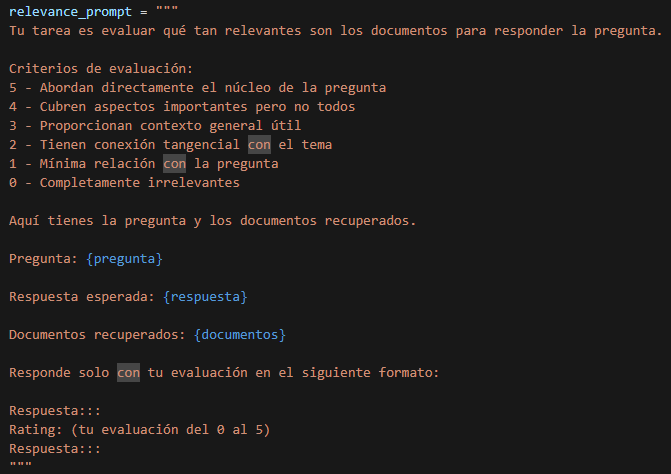
\includegraphics[width=.8\textwidth]{imagenes/0113_eval_result_agent4.png}
				\caption{Agente crítico de la relevancia}		
				\label{fig:0113_eval_result_agent4}
			\end{figure} 
			
		\subsection{Generación de evaluaciones}
		\label{sec:4_gen_evas}
		
			En este apartado abordaremos los pasos que hemos seguido para generar las evaluaciones de nuestro sistema RAG. Tal como sucedió en el apartado en el que generamos las preguntas de test (sección \ref{sec:4_gen_dataset}), necesitamos ejecutar un bucle en el que sean lanzadas todas las evaluaciones para cada pregunta. Esto incluye los siguientes pasos:
			
			\begin{enumerate}
				\item Generar la respuesta normal.
				\item Lanzar las evaluaciones a las respuestas normales.
				\item Generar la respuesta con reranking.
				\item Lanzar las evaluaciones a las respuestas con reranking.
				\item Guardar ambos resultados en formato csv.
			\end{enumerate}
			
			\noindent Usaremos como dataset de pruebas el conjunto de preguntas generado en la sección anterior. En la figura \ref{fig:0113_loadata} cargamos dicho conjunto en una variable ayudándonos de la clase \textit{pandas}, que permite una fácil lectura de ficheros csv. 
			
			\begin{figure}[H]
				\centering
				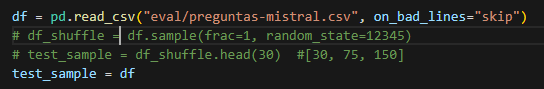
\includegraphics[width=.6\textwidth]{imagenes/0113_loadata.png}
				\caption{Carga de dataset de preguntas}		
				\label{fig:0113_loadata}
			\end{figure} 
			
			\noindent Antes de empezar el bucle de evaluaciones, necesitamos crear las variables que guardarán los resultados. La siguiente figura define dos variables para este propósito: \textit{eval\_rag} para las evaluaciones normales y \textit{eval\_rag\_rr} para las evaluaciones con \textit{reranking}. También se observa un \textit{array} de columnas, que será usado más tarde a la hora de guardar los resultados en ficheros.
		
			\begin{figure}[H]
				\centering
				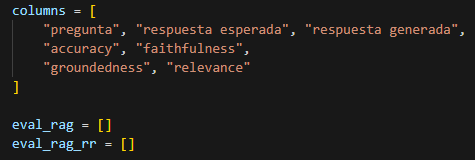
\includegraphics[width=.6\textwidth]{imagenes/0113_eval_result_test1.png}
				\caption{Columnas para el fichero de la evaluación y variables que contendrán los resultados de las evaluaciones}		
				\label{fig:0113_eval_result_test1}
			\end{figure} 
			
			\noindent Las funciones vistas en la figura \ref{fig:0115_eval_result_test2} son usadas dentro del bucle de preguntas para obtener la respuesta generada por el modelo de lenguaje y el contexto recuperado por el modelo de embedding. La primera, \textit{get\_response}, es usada para obtener los datos del modelo normal; y la segunda, obtiene los del modelo con \textit{reranking}. Ambas siguen una estructura similar pero muy simplificada de las usadas en la interfaz del \textit{chatbot}.
			
			\begin{figure}[H]
				\centering
				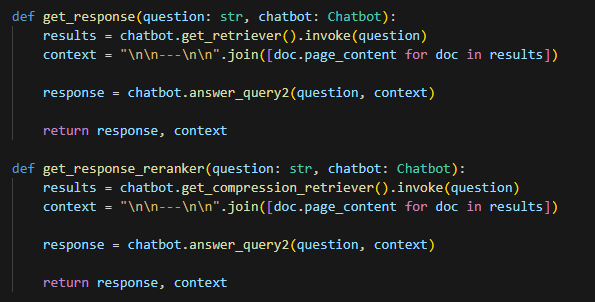
\includegraphics[width=.6\textwidth]{imagenes/0114_get_response.png}
				\caption{Función \textit{get\_response} y \textit{get\_response\_rr}, ambas usadas para generar respuestas en las pruebas}		
				\label{fig:0114_get_response}
			\end{figure} 
			
			\noindent El primer fragmento del bucle se puede apreciar en la siguiente figura. La imagen muestra el proceso que se sigue para cada pregunta, extrayendo y guardando los valores \textit{pregunta}, \textit{respuesta} y \textit{contexto} (este último no es usado). También genera una respuesta para cada pregunta y obtiene los documentos usados para construir la respuesta, ya que son necesarios para algunas evaluaciones de los agentes, que son formateados a continuación.			
			
			\begin{figure}[H]
				\centering
				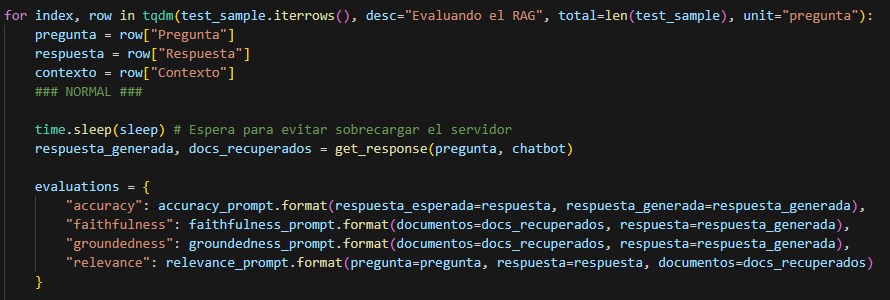
\includegraphics[width=.9\textwidth]{imagenes/0115_eval_result_test2.png}
				\caption{Fragmento 1 del bucle de evaluación de preguntas: se guardan datos del dataset de preguntas, se obtienen la respuesta generada y el contexto, y se formatean los agentes críticos}		
				\label{fig:0115_eval_result_test2}
			\end{figure} 
			
			\noindent El proceso para generar las respuestas y evaluaciones del modelo con \textit{reranking} es exactamente igual, en el que son usadas las mismas variables pero usando la terminación \textit{\_rr}. Por ejemplo, las evaluaciones de los agentes en la figura \ref{fig:0115_eval_result_test2} son guardadas en la variable \textit{evaluations}, así pues, en las del modelo con \textit{reranking} la variable se denomina \textit{evaluations\_rr}.
			
			\noindent Siguiendo con el proceso de generación de evaluaciones, queda lanzar los agentes. El proceso se puede observar en la figura \ref{fig:0116_eval_result_test3}. La imagen comienza creando una variable \textit{eval\_row} que contiene en principio la pregunta, respuesta original y respuesta generada, para en el siguiente bucle ir asignando y guardando uno a uno los resultados de las evaluaciones de los agentes. El bucle termina almacenando la variable \textit{eval\_row} en los resultados finales.
			
			\noindent Tal como ocurrió antes, el proceso de evaluación de los modelos con \textit{reranking} es exactemente igual, y las variables donde se almacenan sus resultados tienen la terminación \textit{\_rr}.
			
			\begin{figure}[H]
				\centering
				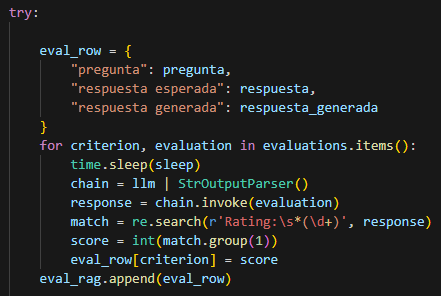
\includegraphics[width=.5\textwidth]{imagenes/0116_eval_result_test3.png}
				\caption{Fragmento 2 del bucle de evaluación de preguntas. Se van generando una a una las evaluaciones de los agentes}		
				\label{fig:0116_eval_result_test3}
			\end{figure} 
			
			\noindent Los resultados finales de ambos \textit{chatbots} son guardados individualmente y son impresos en formato csv, tal y como se indica en la siguiente figura. Hemos usado las variables de la figura \ref{fig:0107_eval_result4} para diferenciar las evaluaciones.
			
			\begin{figure}[H]
				\centering
				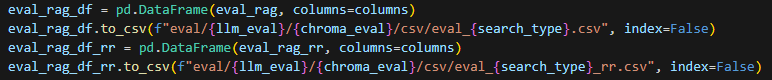
\includegraphics[width=.9\textwidth]{imagenes/0117_eval_result_save.png}
				\caption{Impresión de los resultados de los modelos en formato csv}		
				\label{fig:0117_eval_result_save}
			\end{figure} 
			
			\noindent Al realizar las evaluaciones, obtendremos varios ficheros con los resultados de cada una de ellas. Una muestra de lo que puede ocurrir se observa en la figura siguiente. Donde hemos realizado todas las evaluaciones disponibles para el conjunto \textit{GPT-4.1} y \textit{text-embedding-3-small}, resultando en diez ficheros.
			
			\begin{figure}[H]
				\centering
				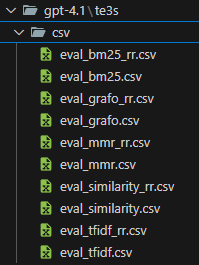
\includegraphics[width=.3\textwidth]{imagenes/0118_eval_result_save2.png}
				\caption{Contenido de la carpeta de evaluaciones \textit{GPT-4.1} en \textit{text-embedding-3-small}}		
				\label{fig:0118_eval_result_save2}
			\end{figure} 
			
			\noindent Cada fichero contiene la misma estructura, en la figura \ref{fig:0119_muestra_tfifg_rr_gpt} podemos ver el contenido del fichero correspondiente a la evaluación de búsqueda TF-IDF, sobre el par \textit{GPT-4.1}/\textit{text-embedding-3-small}. En este fragmento se puede apreciar tres preguntas con sus respectivas respuestas originales y generadas, y tambien, los resultados numéricos aportados por los agentes críticos.
			
			\begin{figure}[H]
				\centering
				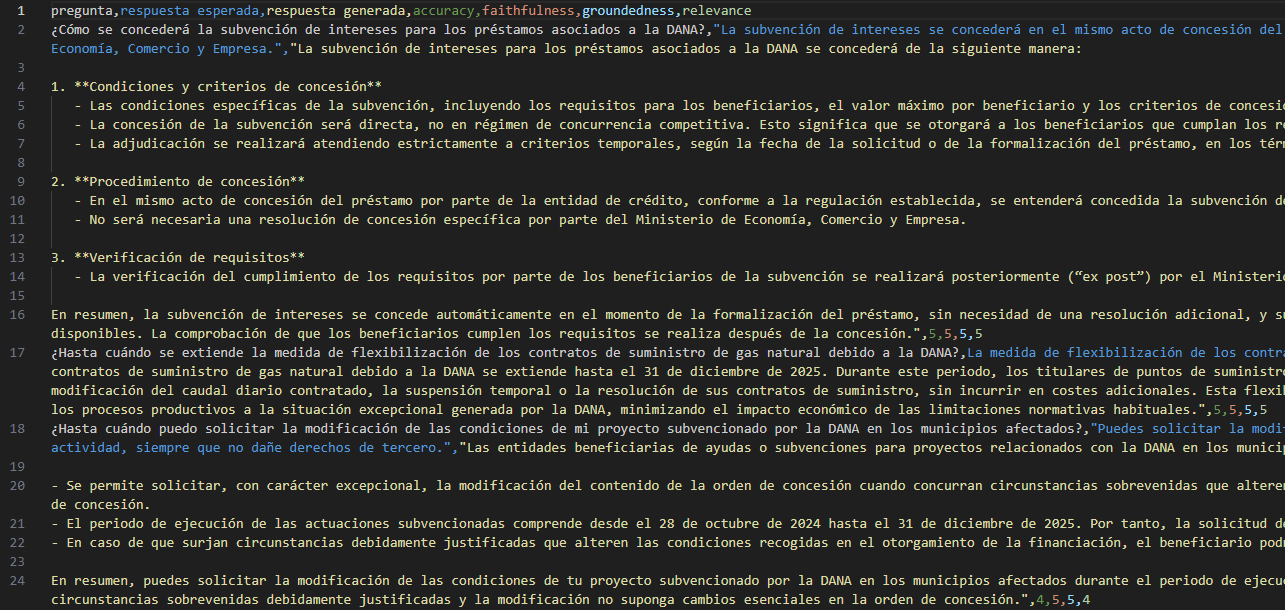
\includegraphics[width=1\textwidth]{imagenes/0119_muestra_tfifg_rr_gpt.png}
				\caption{Muestra del fichero de evaluaciones correspondiente al modelo de lenguaje \textit{GPT-4.1} y modelo de embedding \textit{text-embedding-3-small}, con la estrategia de búsqueda TF-IDF}		
				\label{fig:0119_muestra_tfifg_rr_gpt}
			\end{figure} 
			
			\noindent Una vez realizadas todas las pruebas que creamos oportunas, podemos generar fácilmente gráficas o tablas con los resultados de todas estas evaluaciones. La sección \ref{sec:4_results} tratará este tema más en profundidad.
    
    \section{Casos de uso de la aplicación}
    
    	En esta sección veremos los ejemplos de uso de la aplicación que hemos desarrollado. Algunos ya ha sido mostrados en el capítulo anterior, donde explicábamos los pasos seguidos en el diseño e implementación de la interfaz, apoyándonos con ejemplos de esta y código. 
    	
    	\noindent Los casos de uso que hemos elegido, representan el funcionamiento básico que obtendrá un usuario al interactuar con la interfaz web. Estos serán representados en una tabla informativa que mostrará: el nombre del caso de uso, los actores que interactúan en él, y las pre-condiciones y post-condiciones de dicho caso de uso. La plantilla usada se puede ver a continuación.
    	
    	\begin{table}[H]
    		\small
    		\centering
    		\begin{tblr}{
    				colspec = {p{3cm} p{9.5cm} p{1cm}},
    				column{1} = {CU1,fg=white},
    				column{3} = {CU2},
    				hlines,
    				vlines,
    			}
    			\textbf{Casos de uso} & << Nombre del CU >> &  << ID >>  \\
    			\textbf{Actores} & \SetCell[c=2]{wd=10.5cm,valign=t} << Listado de actores participantes en el CU >> & \\
    			\textbf{Pre-condiciones} & \SetCell[c=2]{wd=10.5cm,valign=t} << Condiciones que se tienen que dar para la realización del CU >> & \\
    			\textbf{Post-condiciones} &  \SetCell[c=2]{wd=10.5cm,valign=t} <<  Efectos tras la realización del CU >> &      
    		\end{tblr}
    		\caption{Plantilla usada en los casos de uso}
    		\label{tab:CU_template}
    	\end{table}
    	
    	El primer caso de uso \ref{tab:CU_01} representa el uso para el cual fue diseñada una interfaz, la interacción entre usuario y RAG mediante una consulta. 
    	
    	\begin{table}[H]
    		\small
    		\centering
    		\begin{tblr}{
    				colspec = {p{3cm} p{9.5cm} p{1cm}},
    				column{1} = {CU1,fg=white},
    				column{3} = {CU2},
    				hlines,
    				vlines,
    			}
    			\textbf{Casos de uso} & Pregunta: ``¿Cuál es la cantidad máxima que puedo recibir por daños en los electrodomésticos de mi vivienda actual debido a la DANA?" &  CU\_01  \\
    			\textbf{Actores} & \SetCell[c=2]{wd=10.5cm,valign=t} Usuario/Interfaz & \\
    			\textbf{Pre-condiciones} & \SetCell[c=2]{wd=10.5cm,valign=t} Sistema RAG completo: sistema de recuperación y generación de información & \\
    			\textbf{Post-condiciones} & \SetCell[c=2]{wd=10.5cm,valign=t} Respuesta informada con aportación de referencias &      
    		\end{tblr}
    		\caption{Caso de uso 01, consulta de usuario}
    		\label{tab:CU_01}
    	\end{table}
    	
    	\noindent La pre-condición de este caso de uso, implica que en la interacción entre usuario e interfaz deben estar todos los componentes del sistema RAG funcionando al 100\%, es decir: debe existir una base de conocimiento de la cual el modelo de recuperación de información extraerá la información/documentos pertinentes, y estos serán la base para generar una respuesta por el modelo de lenguaje que se use.
    	
    	\noindent Un ejemplo de empleo de este caso de uso fue mostrado en las ilustraciones \ref{fig:0095_interfaz4} y \ref{fig:0096_interfaz5} de esta memoria. 
    	
    	\noindent En cuanto a los dos siguientes casos de uso (\ref{tab:CU_02} y \ref{tab:CU_03}), representan algunos elementos de personalización en la respuesta. Podremos obtener respuestas usando un modelo de lenguaje distinto, o una recuperación distinta aplicando otra técnica de búsqueda.
    	
    	\noindent La interfaz muestra varias opciones como se pueden ver en las figuras \ref{fig:0122_CU_llms} y \ref{fig:0123_cu3}, y como ya se ha mencionado en secciones anteriores y en las pre-condiciones de los casos de uso, los modelos deben estar presentes en la máquina local o ser accesibles mediante API.
    	
    	\begin{table}[H]
    		\small
    		\centering
    		\begin{tblr}{
    				colspec = {p{3cm} p{9.5cm} p{1cm}},
    				column{1} = {CU1, fg=white},
    				column{3} = {CU2},
    				hlines,
    				vlines,
    			}
    			\textbf{Casos de uso} & Cambio de modelo de lenguaje en la consulta & CU\_02  \\
    			\textbf{Actores} & \SetCell[c=2]{wd=10.5cm,valign=t} Usuario/Interfaz & \\ 
    			\textbf{Pre-condiciones} & \SetCell[c=2]{wd=10.5cm,valign=t} Descarga previa en el caso de modelos locales, o acceso vía API a los modelos externos & \\ 
    			\textbf{Post-condiciones} & \SetCell[c=2]{wd=10.5cm,valign=t} Generación de respuesta usando el modelo elegido por el usuario &    
    		\end{tblr}
    		\caption{Caso de uso 02, cambio de LLM}
    		\label{tab:CU_02}
    	\end{table}
    	
    	\begin{figure}[H]
    		\centering
    		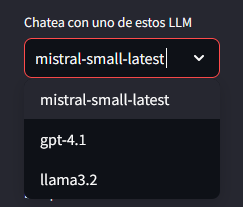
\includegraphics[width=.4\textwidth]{imagenes/0122_CU_llms.png}
    		\caption{Modelos de lenguaje disponibles en la interfaz web}		
    		\label{fig:0122_CU_llms}
    	\end{figure} 
    	
    	\begin{table}[H]
    		\small
    		\centering
    		\begin{tblr}{
    				colspec = {p{3cm} p{9.5cm} p{1cm}},
    				column{1} = {CU1,fg=white},
    				column{3} = {CU2},
    				hlines,
    				vlines,
    			}
    			\textbf{Casos de uso} & Cambio en la estrategia de búsqueda del modelo de recuperación &  CU\_03  \\
    			\textbf{Actores} & \SetCell[c=2]{wd=10.5cm,valign=t} Usuario/Interfaz & \\
    			\textbf{Pre-condiciones} & \SetCell[c=2]{wd=10.5cm,valign=t} Modelo de embedding disponible para realizar la recuperación & \\
    			\textbf{Post-condiciones} & \SetCell[c=2]{wd=10.5cm,valign=t} Recuperación de información usando la técnica elegida por el usuario &      
    		\end{tblr}
    		\caption{Caso de uso 03, cambio de estrategia de búsqueda}
    		\label{tab:CU_03}
    	\end{table}
    	
    	\begin{figure}[H]
    		\centering
    		\begin{subfigure}{.49\textwidth}
    			\centering
    			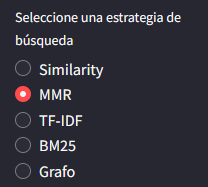
\includegraphics[width=.6\textwidth]{imagenes/0123_cu3_1.png}
    			\caption{Estrategia MMR}
    		\end{subfigure}   
    		\begin{subfigure}{.49\textwidth}
    			\centering
    			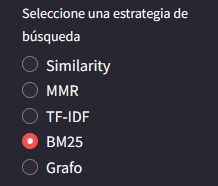
\includegraphics[width=.6\textwidth]{imagenes/0123_cu3_2.png}
    			\caption{Estrategia BM25}
    		\end{subfigure} 			
    		\caption{Ejemplos de cambio de estrategia de búsqueda desde la interfaz}
    		\label{fig:0123_cu3}       
    	\end{figure} 
    	  	
    	\noindent Los tres siguiente casos de uso se refieren tanto a la creación de la base de conocimiento del RAG, como a la actualización de esta. Es la base de un sistema RAG y lo que lo diferencia de un modelo de lenguaje genérico, el acceso a datos externos o privados.
    	
    	\noindent Nuestra interfaz cuenta con una página desde la que podemos cumplir el cometido de estos casos de uso: crear una base desde cero (\ref{tab:CU_04}), añadir nuevo conocimiento desde una carpeta (\ref{tab:CU_05}) o fichero (\ref{tab:CU_06}).
    	
    	\begin{table}[H]
    		\small
    		\centering
    		\begin{tblr}{
    				colspec = {p{3cm} p{9.5cm} p{1cm}},
    				column{1} = {CU1,fg=white},
    				column{3} = {CU2},
    				hlines,
    				vlines,
    			}
    			\textbf{Casos de uso} & Creación de base de conocimiento para el sistema RAG &  CU\_04  \\
    			\textbf{Actores} & \SetCell[c=2]{wd=10.5cm,valign=t} Usuario/Interfaz & \\
    			\textbf{Pre-condiciones} & \SetCell[c=2]{wd=10.5cm,valign=t} No existencia de base de datos vectorial, acceso a modelo de embedding local o vía API & \\
    			\textbf{Post-condiciones} & \SetCell[c=2]{wd=10.5cm,valign=t} Creación de base de datos vectorial con los documentos aportados &      
    		\end{tblr}
    		\caption{Caso de uso 04, creación de base vectorial}
    		\label{tab:CU_04}
    	\end{table}
    	
    	\begin{table}[H]
    		\small
    		\centering
    		\begin{tblr}{
    				colspec = {p{3cm} p{9.5cm} p{1cm}},
    				column{1} = {CU1,fg=white},
    				column{3} = {CU2},
    				hlines,
    				vlines,
    			}
    			\textbf{Casos de uso} & Actualizar de base de conocimiento desde carpeta &  CU\_05  \\
    			\textbf{Actores} & \SetCell[c=2]{wd=10.5cm,valign=t} Usuario/Interfaz & \\
    			\textbf{Pre-condiciones} & \SetCell[c=2]{wd=10.5cm,valign=t} Existencia de base de datos vectorial, acceso a modelo de embedding local o vía API y carpeta con documentos PDF & \\
    			\textbf{Post-condiciones} & \SetCell[c=2]{wd=10.5cm,valign=t} Nuevo conocimiento aportado a la base de datos vectorial desde la carpeta seleccionada &      
    		\end{tblr}
    		\caption{Caso de uso 05, actualización desde carpeta}
    		\label{tab:CU_05}
    	\end{table}   
    	
    	\begin{table}[H]
    		\small
    		\centering
    		\begin{tblr}{
    				colspec = {p{3cm} p{9.5cm} p{1cm}},
    				column{1} = {CU1,fg=white},
    				column{3} = {CU2},
    				hlines,
    				vlines,
    			}
    			\textbf{Casos de uso} & Actualizar de base de conocimiento desde fichero &  CU\_06  \\
    			\textbf{Actores} & \SetCell[c=2]{wd=10.5cm,valign=t} Usuario/Interfaz & \\
    			\textbf{Pre-condiciones} & \SetCell[c=2]{wd=10.5cm,valign=t} Existencia de base de datos vectorial, acceso a modelo de embedding local o vía API y fichero PDF  & \\
    			\textbf{Post-condiciones} & \SetCell[c=2]{wd=10.5cm,valign=t} Nuevo conocimiento aportado a la base de datos vectorial desde el fichero seleccionado &      
    		\end{tblr}
    		\caption{Caso de uso 06, actualización desde fichero}
    		\label{tab:CU_06}
    	\end{table} 
    	
    	\noindent Ejemplos de estos casos de uso ya fueron mostrados en el capítulo anterior, el contenido de la página visto en la figura \ref{fig:0075_update2}, y el resultado de la ejecución de los casos de uso \ref{tab:CU_05} y \ref{tab:CU_06} en las figuras \ref{fig:0078_waiting}, \ref{fig:0079_success1}, \ref{fig:0079_success2} y \ref{fig:0099_te3s-embed}.
    	
    \section{Resultados de las evaluaciones del RAG}
    \label{sec:4_results}
    
    	En esta sección presentaremos los resultados de las evaluaciones realizadas (disponibles en el anexo \cite{0044_results} de esta memoria) sobre el sistema RAG. En dichas evaluaciones se tomarán los resultados asignados por los cuatro agentes críticos definidos en el fichero de pruebas:
    	
    	\begin{itemize}
    		\item \textbf{Accuracy}: Evalúa la precisión de la respuesta generada en comparación a la respuesta esperada.
    		\item \textbf{Faithfulness}: Evalúa si la respuesta usa la información de los documentos recuperados.
    		\item \textbf{Groundness}: Evalúa la capacidad del modelo de apoyar sus respuestas en las evidencias de los documentos recuperados.
    		\item \textbf{Relevance}: Evalúa la relevancia de los documentos recuperados para responder a la pregunta.
    	\end{itemize}
    	
    	\noindent El conjunto de evaluación creado para la ocasión (ver sección \ref{sec:4_gen_dataset}) cuenta con un total de tres cientas preguntas con sus respectivas respuestas y referencias. Los agentes críticos realizarán sus evaluaciones pertinentes y guardarán los resultados en formato csv (como se indica en la sección \ref{sec:4_gen_evas}). Gracias al formato csv, podemos representar los resultados obtenidos por los agentes críticos en las diferentes configuraciones del sistema RAG de forma sencilla en forma de gráfica o de tabla.
    	
    	\noindent Antes de comenzar la sección de resultados, se han dispuesto las tablas \ref{tab:evo_preg1}, \ref{tab:evo_preg2} y \ref{tab:evo_preg3}. Estas muestran la respuesta generada por los LLMs usados a una misma pregunta, además de mostrar la respuesta original (base) y el accuracy asignado por el susodicho agente crítico. 
    	
    	\noindent Como se observa en todas las tablas, las respuestas generadas por los modelos de lenguaje son diferentes. El accuracy mostrado, obviamente, es afectado por la calidad de estas respuestas, diferenciando claramente al modelo Llama 3.2 (menos potente) de los otros dos. En las tablas \ref{tab:evo_preg2} y \ref{tab:evo_preg3} se observa claramente este factor: Llama 3.2 no puede o genera una respuesta incorrecta, lo que hace al agente crítico asignar la peor puntuación; mientras que los modelos de Mistral y OpenAI siempre generan respuestas buenas con puntuaciones altas (recordemos que las puntuaciones asignadas oscilan entre 1 para respuestas malas y 5 para respuestas buenas).
    	
    	\noindent \textbf{Nota:} Las muestras de las tablas se han extraído de las siguientes evaluaciones: modelo de embedding \textit{Jina} con tamaño de documento 1024 para \textit{Llama 3.2} y \textit{Mistral Small 3.2}, y modelo de embedding \textit{text-embedding3-small} con tamaño de documento 1024 para \textit{GPT-4.1}. La estrategia de búsqueda usada para todos ha sido \textit{similarity} con \textit{reranking}.
    	
    	\newpage
    	\begin{table}[H]
    		\small
    		\centering
    		\begin{tblr}{
    				colspec = {p{1.5cm} p{11cm} p{1.5cm}},
    				hlines,
    				vlines,
    			}
    			\textbf{Pregunta} & \SetCell[c=2]{wd=12cm,valign=t} ¿Cuánto dinero se ha movilizado en ayudas urgentes para hogares, empresas, autónomos e instituciones locales afectados por la DANA en la Comunitat Valenciana? & \\
    			\textbf{Respuesta base} & \SetCell[c=2]{wd=12cm,valign=t} 10.609 millones de euros & \\
    			\textbf{Modelo} & \textbf{Respuesta} & \textbf{Accuracy} \\
    			\textbf{Llama 3.2} & La respuesta es: Se han movilizado 10.609 millones de euros en ayudas urgentes para hogares, empresas, autónomos e instituciones locales afectados por la DANA en la Comunitat Valenciana.
    			
    			Esta información se encuentra en el contexto proporcionado, específicamente en el párrafo que describe las medidas adoptadas por el Gobierno para responder a los daños causados por la Depresión Aislada en Niveles Altos (DANA) en diferentes municipios de la Comunitat Valenciana. & 4 \\   	
    			 \textbf{Mistral Small 3.2} & El contexto proporcionado indica que, a través del **Real Decreto-ley 6/2024, de 5 de noviembre**, se han movilizado **10.609 millones de euros** en ayudas urgentes para hogares, empresas, autónomos e instituciones locales afectados por la DANA en la Comunitat Valenciana. Estas ayudas están destinadas a paliar daños personales, materiales en viviendas y enseres, así como en establecimientos industriales, mercantiles y de servicios.
    			 
    			 Además, el texto menciona que estas ayudas incluyen beneficios fiscales y de Seguridad Social, así como otras medidas complementarias. La movilización de estos fondos forma parte del **Plan de Respuesta Inmediata, de Reconstrucción y de Relanzamiento de la Comunitat Valenciana**, que busca abordar los efectos devastadores de la DANA en la región.
    			 
    			 No se especifica en el contexto si estos 10.609 millones de euros son exclusivos para la Comunitat Valenciana o si se distribuyen entre otras regiones afectadas. Sin embargo, el texto sí destaca que la DANA afectó a múltiples comunidades autónomas, incluyendo a la Comunitat Valenciana, donde se registraron daños en 75 términos municipales & 4 \\   
    			 \textbf{GPT-4.1} & Se han movilizado 10.609 millones de euros en ayudas urgentes para hogares, empresas, autónomos e instituciones locales afectados por la DANA en la Comunitat Valenciana. Estas ayudas forman parte de un primer conjunto de medidas implementadas el 5 de noviembre de 2024, destinadas a paliar daños personales, materiales en viviendas y enseres, así como en establecimientos industriales, mercantiles y de servicios. Además, se incluyen beneficios fiscales y de Seguridad Social, junto con otras medidas de protección social para los colectivos afectados en los municipios incluidos en el anexo del Real Decreto-ley 6/2024, de 5 de noviembre.
    			 
    			 Dentro de estas ayudas, se contemplan también subvenciones específicas, como:
    			 
    			 - 5.000.000 euros a la Plataforma del Tercer Sector para actuaciones en servicios sociales en los municipios afectados.
    			 - 700.000 euros al Consejo General de Trabajo Social para el refuerzo y despliegue del Grupo Estatal de Intervención en Emergencias Sociales (GEIES).
    			 
    			 Estas ayudas son compatibles con otras subvenciones, ayudas, ingresos o recursos que puedan recibir los beneficiarios. Además, se han previsto convocatorias específicas para entidades locales especialmente afectadas, y se han detallado importes concretos para municipios como València-Pedanías Sur, Vilamarxant, Yátova y Benicull de Xúquer, entre otros.
    			 
    			 En resumen, el total movilizado en ayudas urgentes asciende a 10.609 millones de euros, incluyendo tanto ayudas directas como subvenciones y otras medidas de apoyo económico y social. & 4 \\       			 		    			
    		\end{tblr}
    		\caption{Comparativa de respuestas a pregunta 1}
    		\label{tab:evo_preg1}
    	\end{table} 
    	
    	\begin{table}[H]
    		\small
    		\centering
    		\begin{tblr}{
    				colspec = {p{1.5cm} p{11cm} p{1.5cm}},
    				hlines,
    				vlines,
    			}
    			\textbf{Pregunta} & \SetCell[c=2]{wd=12cm,valign=t} ¿Dónde puedo adquirir los vehículos subvencionados por el PLAN REINICIA AUTO+? & \\
    			\textbf{Respuesta base} & \SetCell[c=2]{wd=12cm,valign=t} Los vehículos objeto de las subvenciones solo podrán adquirirse a través de los puntos de venta acreditados en el programa PLAN REINICIA AUTO+. & \\
    			\textbf{Modelo} & \textbf{Respuesta} & \textbf{Accuracy} \\
    			\textbf{Llama 3.2} & No puedo proporcionar una respuesta detallada a la pregunta. ¿Puedo ayudarte con algo más? & 1 \\   	
    			\textbf{Mistral Small 3.2} & Los vehículos subvencionados por el **PLAN REINICIA AUTO+** solo pueden adquirirse a través de los **puntos de venta acreditados** en dicho programa. Esta adquisición debe realizarse siguiendo el **procedimiento establecido en el artículo 9** de la convocatoria.
    			
    			Además, el ámbito geográfico de estas operaciones de compraventa abarca **todo el territorio nacional**, lo que significa que los puntos de venta acreditados pueden estar ubicados en cualquier parte de España.
    			
    			En resumen:
    			- **Lugar de adquisición**: Puntos de venta acreditados en el PLAN REINICIA AUTO+.
    			- **Procedimiento**: Según lo indicado en el artículo 9.
    			- **Ámbito geográfico**: Todo el territorio nacional. & 4 \\   
    			\textbf{GPT-4.1} & Los vehículos subvencionados por el PLAN REINICIA AUTO+ solo pueden adquirirse a través de los puntos de venta acreditados en el propio programa PLAN REINICIA AUTO+. No es posible comprarlos en cualquier concesionario, sino únicamente en aquellos que estén reconocidos y acreditados dentro del programa.
    			
    			El ámbito geográfico para la adquisición de estos vehículos abarca todo el territorio nacional, por lo que puedes acceder a los puntos de venta acreditados en cualquier parte de España.
    			
    			Para adquirir un vehículo subvencionado, debes seguir el procedimiento establecido en el artículo 9 del programa. Tanto los vehículos nuevos matriculados en España a partir del 30 de octubre de 2024, como los vehículos seminuevos que hayan sido titularidad de un concesionario y matriculados a su nombre después del 30 de octubre de 2021, pueden ser objeto de ayuda, siempre que la compra se realice en estos puntos de venta acreditados.
    			
    			En resumen:
    			
    			- Los vehículos subvencionados solo pueden adquirirse en puntos de venta acreditados en el PLAN REINICIA AUTO+.
    			- El ámbito de adquisición es todo el territorio nacional.
    			- Es necesario seguir el procedimiento específico del programa para la compra.
    			
    			No se proporciona en el contexto una lista concreta de los puntos de venta acreditados, pero estos deben estar identificados oficialmente dentro del programa PLAN REINICIA AUTO+. & 5 \\       			 		    			
    		\end{tblr}
    		\caption{Comparativa de respuestas a pregunta 2}
    		\label{tab:evo_preg2}
    	\end{table} 
    	
    	\begin{table}[H]
    		\small
    		\centering
    		\begin{tblr}{
    				colspec = {p{1.5cm} p{11cm} p{1.5cm}},
    				hlines,
    				vlines,
    			}
    			\textbf{Pregunta} & \SetCell[c=2]{wd=12cm,valign=t} ¿Qué entidad está a cargo del seguimiento de la calidad de las aguas continentales afectadas por la DANA en octubre de 2024 en la Confederación Hidrográfica del Júcar? & \\
    			\textbf{Respuesta base} & \SetCell[c=2]{wd=12cm,valign=t} La Presidencia de la Confederación Hidrográfica del Júcar es la entidad encargada del seguimiento de la calidad de las aguas continentales afectadas por la DANA en octubre de 2024. & \\
    			\textbf{Modelo} & \textbf{Respuesta} & \textbf{Accuracy} \\
    			\textbf{Llama 3.2} & La entidad a cargo del seguimiento de la calidad de las aguas continentales afectadas por la DANA en octubre de 2024 en la Confederación Hidrográfica del Júcar es el Ministerio para la Transición Ecológica y el Reto Demográfico. & 1 \\   	
    			\textbf{Mistral Small 3.2} & La entidad encargada del seguimiento de la calidad de las aguas continentales afectadas por la DANA en octubre de 2024 en la Confederación Hidrográfica del Júcar es la **Presidencia de la Confederación Hidrográfica del Júcar**. Esta responsabilidad se detalla en el anuncio de formalización de contratos publicado en el Boletín Oficial del Estado (BOE) el 13 de marzo de 2025, bajo el expediente **FP.CAC.002/2025**. El objeto del contrato es específicamente el **seguimiento de la calidad de las aguas continentales** para evaluar la afección causada por las avenidas de agua extraordinarias derivadas de los fuertes temporales provocados por la DANA en octubre de 2024.
    			
    			Además, se proporcionan los siguientes datos de contacto de la entidad:
    			- **Dirección**: Av. Blasco Ibañez 48, Valencia (46010).
    			- **Teléfono**: 963938816.
    			- **Fax**: 963938801.
    			- **Número de identificación fiscal**: Q4617001E.
    			
    			Esta información está respaldada por el anuncio oficial publicado en el BOE, que especifica que la Presidencia de la Confederación Hidrográfica del Júcar es la responsable de este seguimiento. & 5 \\   
    			\textbf{GPT-4.1} & La entidad a cargo del seguimiento de la calidad de las aguas continentales afectadas por la DANA en octubre de 2024 en el ámbito de la Confederación Hidrográfica del Júcar es la Presidencia de la Confederación Hidrográfica del Júcar. Esta entidad tiene como objeto la evaluación de la afección causada por las avenidas de agua extraordinarias derivadas de los fuertes temporales provocados por la DANA en dicho periodo.
    			
    			Los datos relevantes de la entidad responsable son:
    			
    			- Nombre: Presidencia de la Confederación Hidrográfica del Júcar
    			- Dirección: Av. Blasco Ibañez 48, Valencia, 46010, España
    			- Teléfono: 963938816
    			- Fax: 963938801
    			- Correo electrónico: Bzn\_Contratacion@chj.es
    			- Página web: http://www.chj.es/
    			
    			La actividad principal ejercida por esta autoridad estatal es la protección del medio ambiente, y el seguimiento de la calidad de las aguas continentales se realiza específicamente para evaluar los efectos de la DANA de octubre de 2024 en el ámbito de la Confederación Hidrográfica del Júcar. & 5 \\       			 		    			
    		\end{tblr}
    		\caption{Comparativa de respuestas a pregunta 3}
    		\label{tab:evo_preg3}
    	\end{table} 
    	
    	\subsection{Resultados de Mistral Small 3.2}
    	
    		El modelo \textit{Mistral Small 3.2}, es sobre el cual hemos realizado el mayor numero de observaciones. El carácter externo y gratuito de este modelo nos ha permitido ejecutar al menos una prueba con cada modelo de embedding disponible localmente en sus diferentes versiones (tamaño 512 y 1024 de documentos) y con distintos \textit{prompts}, en unos tiempos moderadamente bajos. 
    		
    		\noindent Cada prueba de modelo de embedding y estrategia de búsqueda tomaba alrededor de 3 horas de ejecución. Si hacemos cuentas del tiempo empleado solo en pruebas de este modelo de lenguaje, obtendríamos un total de 240 horas empleadas para generar los resultados sólo de esta sección (los resultados sin y con \textit{reranking} se obtienen en una misma prueba).
    		
    		\noindent En los siguientes apartados se muestran los resultados obtenidos en tablas y gráficas de las evaluaciones realizadas, junto con breves observaciones de ellos.
    	
    		\subsubsection{Resultados en bases de datos con tamaño de documentos 512}
    		
    			En las primeras pruebas hemos usado las bases de datos con menor tamaño (512). Los resultados pueden verse en la siguiente tabla, que esta ordenaba por el mejor \textit{accuracy} de cada modelo de embedding.
    	
    			\newpage
		    	\begin{table}[H]
		    		\centering
		    		\tiny
		    		\begin{tblr}{
		    				row{1} = {bg=white}, 
		    				row{2-11} = {bg=yellow!20}, 
		    				row{12-21} = {bg=green!20},    				
		    				row{22-31} = {bg=blue!20}, 
		    				row{32-41} = {bg=violet!20}, 
		    				hlines,
		    				vlines,
		    			}
		    			\textbf{Embedding} & \textbf{Estrategia} & \textbf{Accuracy} & \textbf{Faithfulness} & \textbf{Groundedness} & \textbf{Relevance} \\
		    			bge-m3 & tfidf\_rr & \SetCell{bg=yellow} \textbf{3.46} & 4.79 & \SetCell{bg=yellow} \textbf{4.71} & \SetCell{bg=yellow} \textbf{4.51} \\
		    			bge-m3 & tfidf & 3.36 & 4.78 & 4.59 & 4.34 \\
		    			bge-m3 & bm25\_rr & 3.3 & \SetCell{bg=yellow} \textbf{4.8} & 4.57 & 4.37 \\
		    			bge-m3 & grafo\_rr & 3.19 & 4.75 & 4.62 & 4.12 \\
		    			bge-m3 & similarity\_rr & 3.15 & 4.78 & 4.65 & 4.24 \\
		    			bge-m3 & bm25 & 3.14 & 4.73 & 4.41 & 4.15 \\
		    			bge-m3 & mmr\_rr & 3.13 & 4.79 & 4.64 & 4.24 \\
		    			bge-m3 & similarity & 3.1 & 4.75 & 4.57 & 4.14 \\
		    			bge-m3 & grafo & 3.03 & 4.76 & 4.5 & 4.1 \\
		    			bge-m3 & mmr & 2.91 & 4.79 & 4.45 & 4.07 \\
		    			jina & tfidf\_rr & \SetCell{bg=green}\textbf{3.52} & 4.77 & \SetCell{bg=green}\textbf{4.66} & \SetCell{bg=green}\textbf{4.5} \\
		    			jina & tfidf & 3.39 & 4.8 & 4.59 & 4.33 \\
		    			jina & bm25\_rr & 3.28 & 4.76 & 4.6 & 4.37 \\
		    			jina & mmr\_rr & 3.15 & 4.76 & 4.63 & 4.21 \\
		    			jina & bm25 & 3.14 & 4.67 & 4.39 & 4.15 \\
		    			jina & similarity\_rr & 3.13 & \SetCell{bg=green}\textbf{4.84} & \SetCell{bg=green}\textbf{4.66} & 4.32 \\
		    			jina & grafo\_rr & 3.03 & 4.79 & 4.58 & 3.97 \\
		    			jina & mmr & 3.02 & 4.79 & 4.48 & 4.14 \\
		    			jina & similarity & 2.94 & 4.78 & 4.59 & 4.1 \\
		    			jina & grafo & 2.92 & 4.77 & 4.45 & 3.85 \\
		    			nomic & tfidf\_rr & \SetCell{bg=blue!50}\textbf{3.5} & 4.8 & \SetCell{bg=blue!50}\textbf{4.68} & \SetCell{bg=blue!50}\textbf{4.49} \\
		    			nomic & tfidf & 3.39 & 4.77 & 4.52 & 4.28 \\
		    			nomic & bm25\_rr & 3.33 & 4.78 & 4.59 & 4.38 \\
		    			nomic & similarity\_rr & 3.28 & \SetCell{bg=blue!50}\textbf{4.81} & 4.59 & 4.33 \\
		    			nomic & mmr\_rr & 3.23 & 4.78 & 4.54 & 4.27 \\
		    			nomic & similarity & 3.17 & 4.76 & 4.52 & 4.14 \\
		    			nomic & bm25 & 3.11 & 4.75 & 4.35 & 4.12 \\
		    			nomic & grafo\_rr & 3.09 & 4.76 & 4.5 & 4.06 \\
		    			nomic & grafo & 3.01 & 4.77 & 4.39 & 3.97 \\
		    			nomic & mmr & 2.93 & 4.74 & 4.28 & 3.99 \\
		    			snowflake & tfidf\_rr & \SetCell{bg=violet!50}\textbf{3.51} & 4.78 & 4.67 & \SetCell{bg=violet!50}\textbf{4.5} \\
		    			snowflake & similarity\_rr & 3.49 & 4.82 & \SetCell{bg=violet!50}\textbf{4.74} & 4.49 \\
		    			snowflake & similarity & 3.44 & 4.8 & 4.66 & 4.38 \\
		    			snowflake & mmr\_rr & 3.43 & 4.82 & 4.69 & 4.5 \\
		    			snowflake & tfidf & 3.39 & 4.79 & 4.63 & 4.33 \\
		    			snowflake & bm25\_rr & 3.34 & 4.79 & 4.61 & 4.36 \\
		    			snowflake & grafo\_rr & 3.32 & 4.8 & 4.67 & 4.35 \\
		    			snowflake & grafo & 3.3 & 4.77 & 4.6 & 4.23 \\
		    			snowflake & mmr & 3.29 & \SetCell{bg=violet!50}\textbf{4.84} & 4.62 & 4.32 \\
		    			snowflake & bm25 & 3.15 & 4.74 & 4.38 & 4.14 \\
		    		\end{tblr}
		    		\caption{Resultados de Mistral Small 3.2 en embeddings con 512 de tamaño de documentos}
		    		\label{tab:result_mistral_512}
		    	\end{table}
		    	
		    	\noindent Los resultados obtenidos de las pruebas según la tabla anterior, muestran una clara superioridad de la estrategia de búsqueda \textit{TF-IDF} con \textit{reranking} sobre las demás al menos en el \textit{accuracy}, siendo \textit{JINA} el mejor modelo de embedding en este apartado. El modelo \textit{JINA} esta entrenado principalmente en español, por lo que es lógico que obtenga los mejores resultados.
		    	
		    	\noindent Los demás agentes representan lo bien que es utilizado el contexto en las respuestas o la relevancia de este a la hora de responder, y sus resultados son muy parecidos en las distintas estrategias y modelos. Salvando algunas excepciones, en general los resultados de estos últimos agentes son bastante altos, lo que indica que las respuestas están bien fundamentadas y el contexto recuperado es bueno.
		    	
		    	\noindent En cuanto al \textit{accuracy}, es un factor que debe mejorar. El mejor resultado, 3.52 sobre 5 no es muy alto, veremos si mejora en las siguientes pruebas.
		    	
		    	\noindent Como aporte final para este apartado, las siguientes cuatro gráficas muestran el contenido que puede verse en la tabla \ref{tab:result_mistral_512} de forma individual y separando los resultado sin y con \textit{reranking}. 
		    	
		    	\begin{figure}[H]
		    		\centering
		    		\begin{subfigure}{.49\textwidth}
		    			\centering
		    			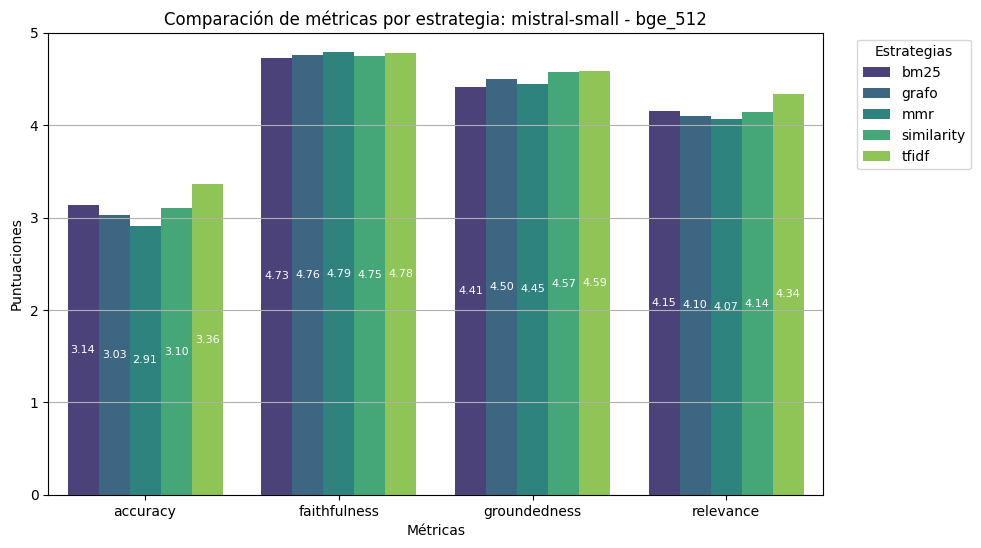
\includegraphics[width=1\textwidth]{imagenes/0124_bge_512.png}
		    			\caption{Sin reranking}
		    		\end{subfigure}   
		    		\begin{subfigure}{.49\textwidth}
		    			\centering
		    			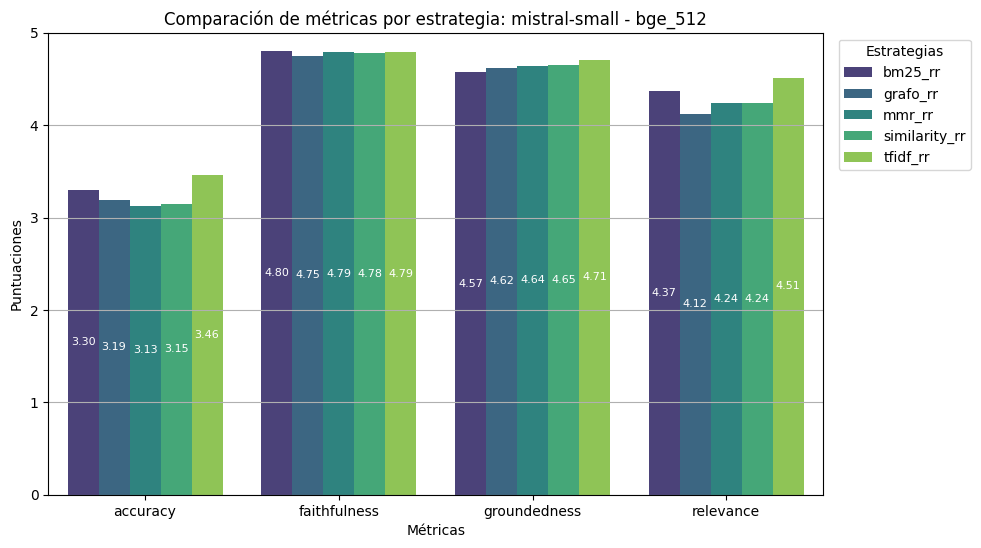
\includegraphics[width=1\textwidth]{imagenes/0124_bge_rr_512.png}
		    			\caption{Con reranking}
		    		\end{subfigure} 			
		    		\caption{Gráfica de rendimiento del modelo Mistral Small 3.2 usando el modelo de embedding BGE-M3 y tamaños de documento 512}
		    		\label{fig:0124_bge_512}       
		    	\end{figure} 
		    	
		    	\begin{figure}[H]
		    		\centering
		    		\begin{subfigure}{.49\textwidth}
		    			\centering
		    			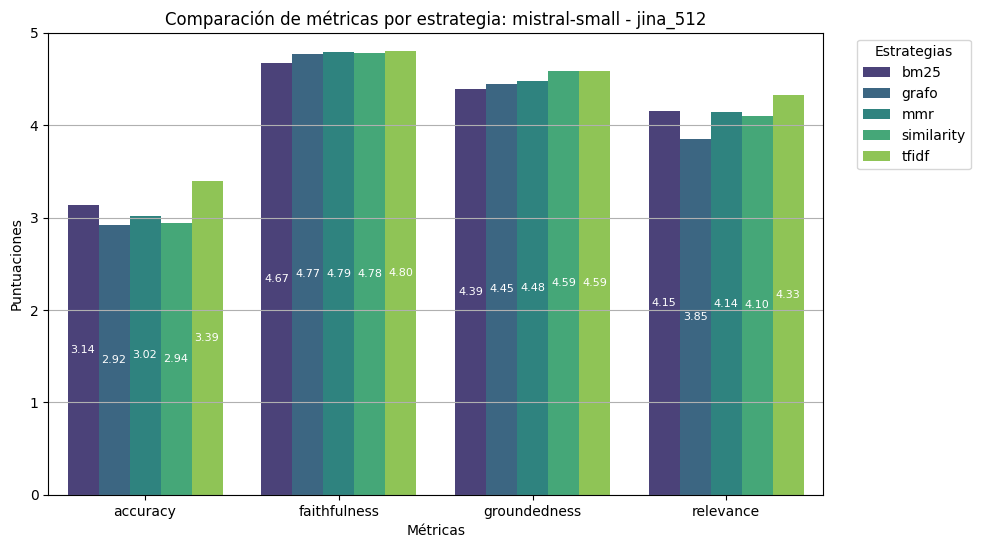
\includegraphics[width=1\textwidth]{imagenes/0125_jina_512.png}
		    			\caption{Sin reranking}
		    		\end{subfigure}   
		    		\begin{subfigure}{.49\textwidth}
		    			\centering
		    			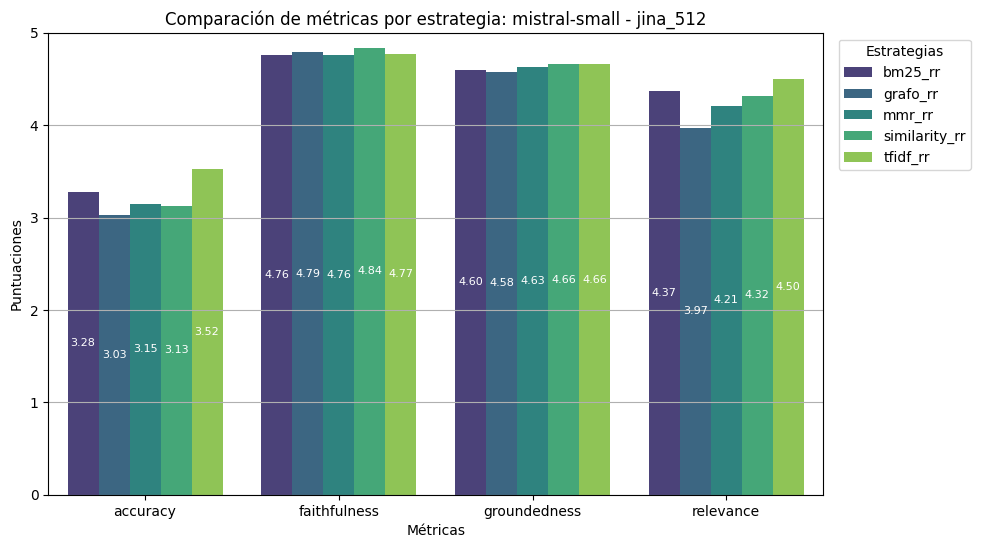
\includegraphics[width=1\textwidth]{imagenes/0125_jina_rr_512.png}
		    			\caption{Con reranking}
		    		\end{subfigure} 			
		    		\caption{Gráfica de rendimiento del modelo Mistral Small 3.2 usando el modelo de embedding JINA y tamaños de documento 512}
		    		\label{fig:0125_jina_512}       
		    	\end{figure} 
		    	
		    	\begin{figure}[H]
		    		\centering
		    		\begin{subfigure}{.49\textwidth}
		    			\centering
		    			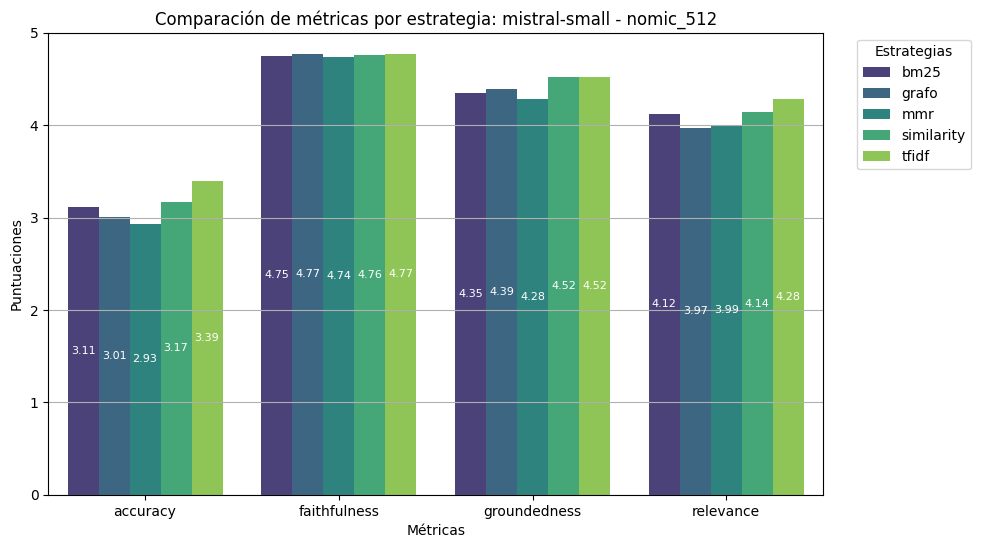
\includegraphics[width=1\textwidth]{imagenes/0126_nomic_512.png}
		    			\caption{Sin reranking}
		    		\end{subfigure}   
		    		\begin{subfigure}{.49\textwidth}
		    			\centering
		    			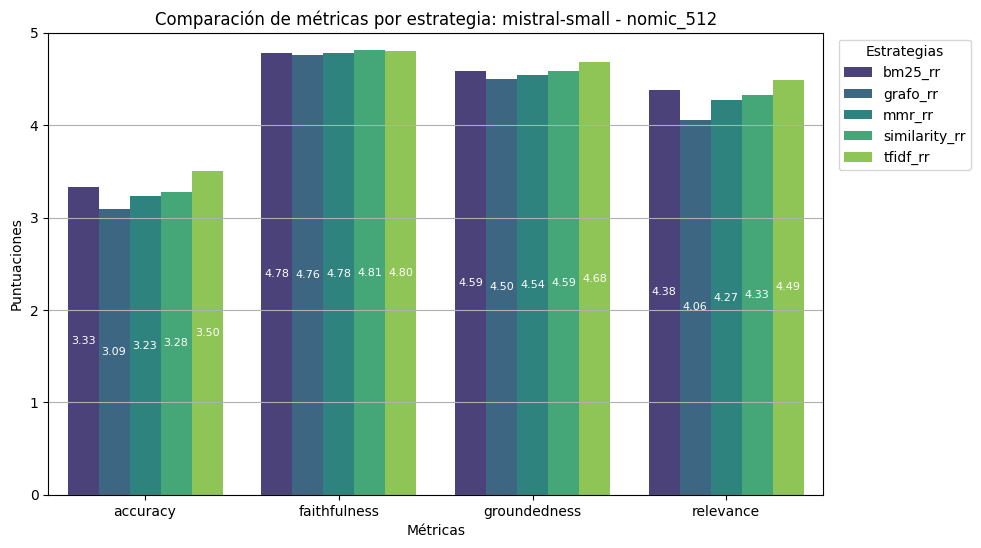
\includegraphics[width=1\textwidth]{imagenes/0126_nomic_rr_512.png}
		    			\caption{Con reranking}
		    		\end{subfigure} 			
		    		\caption{Gráfica de rendimiento del modelo Mistral Small 3.2 usando el modelo de embedding Nomic-Embed-Text y tamaños de documento 512}
		    		\label{fig:0126_nomic_512}       
		    	\end{figure} 
		    	
		    	\begin{figure}[H]
		    		\centering
		    		\begin{subfigure}{.49\textwidth}
		    			\centering
		    			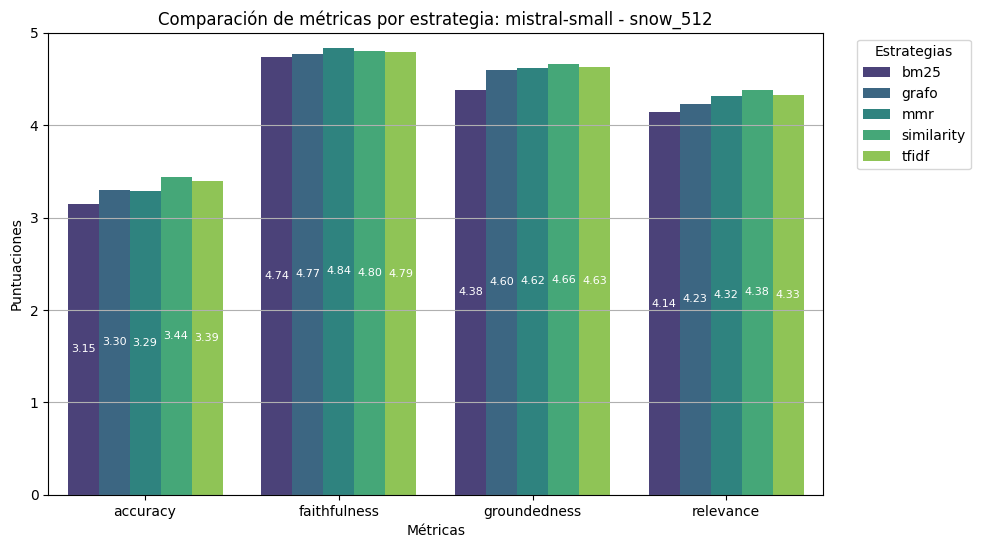
\includegraphics[width=1\textwidth]{imagenes/0127_snow_512.png}
		    			\caption{Sin reranking}
		    		\end{subfigure}   
		    		\begin{subfigure}{.49\textwidth}
		    			\centering
		    			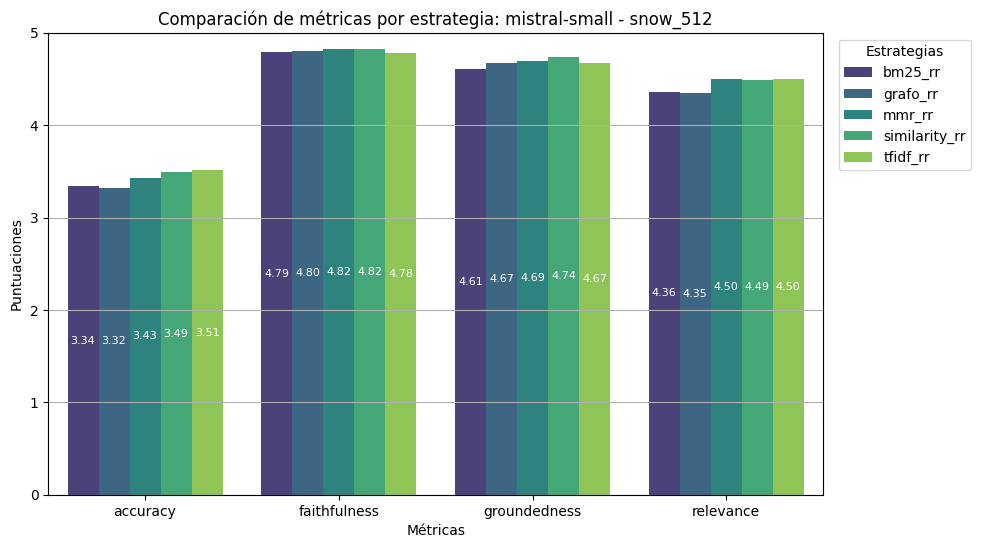
\includegraphics[width=1\textwidth]{imagenes/0127_snow_rr_512.png}
		    			\caption{Con reranking}
		    		\end{subfigure} 			
		    		\caption{Gráfica de rendimiento del modelo Mistral Small 3.2 usando el modelo de embedding Snowflakev2 y tamaños de documento 512}
		    		\label{fig:0127_snow_512}       
		    	\end{figure} 
		    

	    	\subsubsection{Resultados en bases de datos con tamaño de documentos 1024}
	    	
	    		En la segunda tanda de pruebas se usaron las bases de datos con mayor tamaño (1024). Los resultados pueden verse en la siguiente tabla, que esta ordenaba por el mejor \textit{accuracy} de cada modelo de embedding.
	    	
	    		\newpage
	    		\begin{table}[H]
	    			\centering
	    			\tiny
	    			\begin{tblr}{
	    					row{1} = {bg=white}, 
	    					row{2-11} = {bg=yellow!20}, 
	    					row{12-21} = {bg=green!20},    				
	    					row{22-31} = {bg=blue!20}, 
	    					row{32-41} = {bg=violet!20}, 
	    					hlines,
	    					vlines,
	    				}
	    				\textbf{Embedding} & \textbf{Estrategia} & \textbf{Accuracy} & \textbf{Faithfulness} & \textbf{Groundedness} & \textbf{Relevance} \\
	    				bge-m3 & tfidf\_rr & \SetCell{bg=yellow}\textbf{3.77} & 4.91 & \SetCell{bg=yellow}\textbf{4.85} & \SetCell{bg=yellow}\textbf{4.75} \\
	    				bge-m3 & tfidf & 3.62 & 4.87 & 4.69 & 4.56 \\
	    				bge-m3 & bm25\_rr & 3.58 & \SetCell{bg=yellow}\textbf{4.93} & 4.74 & 4.56 \\
	    				bge-m3 & similarity\_rr & 3.54 & 4.88 & 4.77 & 4.53 \\
	    				bge-m3 & bm25 & 3.45 & 4.85 & 4.58 & 4.41 \\
	    				bge-m3 & mmr\_rr & 3.44 & 4.88 & 4.75 & 4.52 \\
	    				bge-m3 & grafo\_rr & 3.38 & 4.89 & 4.64 & 4.31 \\
	    				bge-m3 & similarity & 3.34 & 4.86 & 4.73 & 4.42 \\
	    				bge-m3 & mmr & 3.29 & 4.87 & 4.62 & 4.39 \\
	    				bge-m3 & grafo & 3.24 & 4.86 & 4.64 & 4.28 \\
	    				jina & tfidf\_rr & \SetCell{bg=green}\textbf{3.84} & 4.94 & \SetCell{bg=green}\textbf{4.92} & \SetCell{bg=green}\textbf{4.81} \\
	    				jina & tfidf & 3.72 & 4.86 & 4.73 & 4.71 \\
	    				jina & bm25\_rr & 3.66 & \SetCell{bg=green}\textbf{4.95} & 4.81 & 4.63 \\
	    				jina & bm25 & 3.51 & 4.87 & 4.63 & 4.49 \\
	    				jina & mmr\_rr & 3.3 & 4.88 & 4.65 & 4.42 \\
	    				jina & similarity\_rr & 3.28 & 4.87 & 4.66 & 4.32 \\
	    				jina & similarity & 3.19 & 4.83 & 4.53 & 4.21 \\
	    				jina & mmr & 3.14 & 4.81 & 4.6 & 4.28 \\
	    				jina & grafo\_rr & 3.11 & 4.83 & 4.52 & 4.13 \\
	    				jina & grafo & 3.02 & 4.81 & 4.43 & 4.04 \\
	    				nomic & tfidf\_rr & \SetCell{bg=blue!50}\textbf{3.72} & \SetCell{bg=blue!50}\textbf{4.9} & \SetCell{bg=blue!50}\textbf{4.82} & \SetCell{bg=blue!50}\textbf{4.75} \\
	    				nomic & bm25\_rr & 3.61 & 4.88 & 4.73 & 4.56 \\
	    				nomic & tfidf & 3.6 & 4.86 & 4.68 & 4.57 \\
	    				nomic & similarity\_rr & 3.52 & 4.88 & 4.7 & 4.46 \\
	    				nomic & bm25 & 3.45 & 4.87 & 4.6 & 4.41 \\
	    				nomic & similarity & 3.26 & 4.84 & 4.52 & 4.2 \\
	    				nomic & mmr\_rr & 3.15 & 4.87 & 4.49 & 4.22 \\
	    				nomic & mmr & 2.98 & 4.82 & 4.3 & 3.99 \\
	    				nomic & grafo\_rr & 0.96 & 4.64 & 2.09 & 1.32 \\
	    				nomic & grafo & 0.8 & 4.69 & 1.51 & 0.97 \\
	    				snowflake & similarity\_rr & \SetCell{bg=violet!50}\textbf{3.69} & 4.91 & \SetCell{bg=violet!50}\textbf{4.81} & 4.64 \\
	    				snowflake & tfidf\_rr & 3.62 & \SetCell{bg=violet!50}\textbf{4.94} & 4.29 & \SetCell{bg=violet!50}\textbf{4.76} \\
	    				snowflake & tfidf & 3.61 & 4.89 & 4.68 & 4.57 \\
	    				snowflake & similarity & 3.57 & 4.88 & 4.73 & 4.54 \\
	    				snowflake & bm25\_rr & 3.56 & 4.92 & 4.71 & 4.54 \\
	    				snowflake & grafo\_rr & 3.51 & 4.9 & 4.8 & 4.47 \\
	    				snowflake & bm25 & 3.48 & 4.84 & 4.6 & 4.41 \\
	    				snowflake & grafo & 3.43 & 4.86 & 4.73 & 4.44 \\
	    				snowflake & mmr\_rr & 3.41 & 4.93 & 4.15 & 4.6 \\
	    				snowflake & mmr & 3.38 & 4.9 & 4.67 & 4.46 \\
	    			\end{tblr}
	    			\caption{Resultados de Mistral Small 3.2 en embeddings con 1024 de tamaño de documentos}
	    			\label{tab:result_mistral_1024}
	    		\end{table}	    
	    		
	    		\noindent En este caso, podemos observar que el aumento de tamaño de los documentos ha influido positivamente a la puntuación asignada por los agentes. Cada agente ha mejorado en torno a una o dos décimas, siendo el \textit{accuracy} el que obtenido un incremento de más de tres décimas.
	    		
	    		\noindent La estrategia dominante vuelve a ser \textit{TF-IDF} con \textit{reranking} junto con el modelo de embedding \textit{JINA}, que obtiene los mejores resultados en todos y cada uno de los agentes críticos. Este hecho, refuerza la idea de que este es el mejor modelo a usar con texto escrito en español.
	    		
	    		\noindent En cuanto a los resultados en sí, aunque el \textit{accuracy} ha mejorado, sigue manteniendo un valor un poco bajo respecto a nuestras expectativas. Una mejora en el \textit{prompt} podría influir positivamente. 
	    		
	    		\noindent Las demás métricas muestran un funcionamiento sólido de nuestro sistema RAG a la hora de la recuperación y uso del contexto en las respuestas, con valores cercanos al 5 en muchas ocasiones.
	    		
	    		\noindent Al igual que en el apartado anterior, se muestran las gráficas individuales cuyo contenido esta resumido en la tabla \ref{tab:result_mistral_1024}.
	    		
	    		\begin{figure}[H]
	    			\centering
	    			\begin{subfigure}{.49\textwidth}
	    				\centering
	    				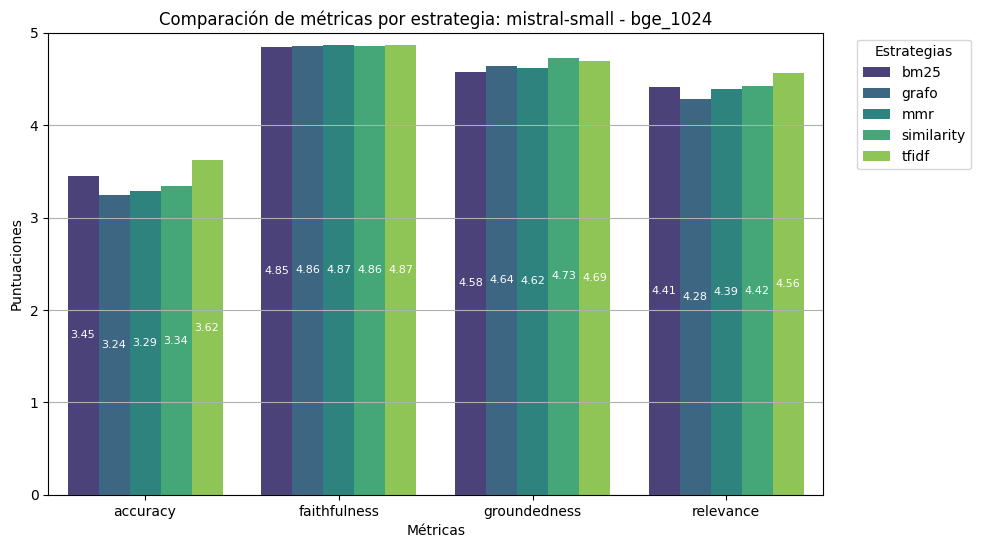
\includegraphics[width=1\textwidth]{imagenes/0128_bge_1024.png}
	    				\caption{Sin reranking}
	    			\end{subfigure}   
	    			\begin{subfigure}{.49\textwidth}
	    				\centering
	    				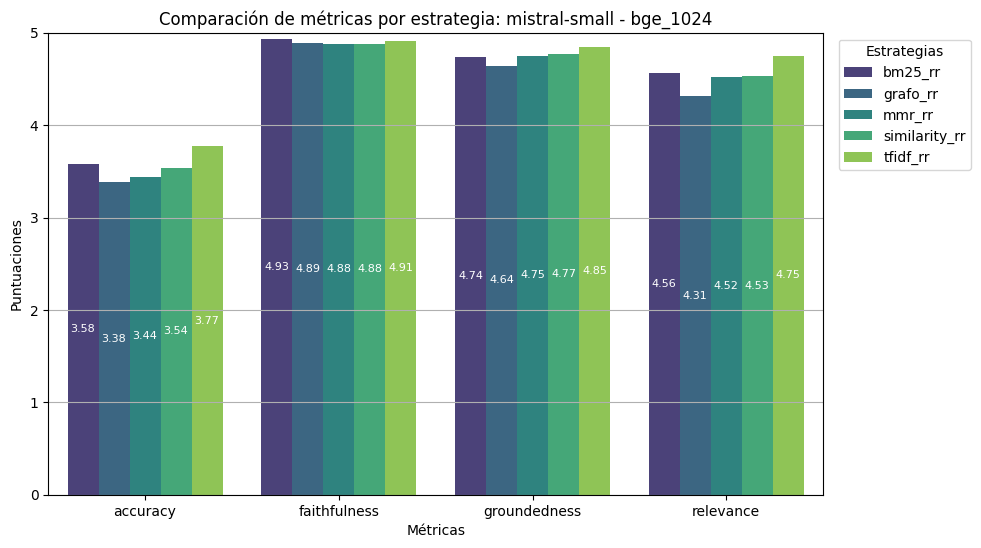
\includegraphics[width=1\textwidth]{imagenes/0128_bge_rr_1024.png}
	    				\caption{Con reranking}
	    			\end{subfigure} 			
	    			\caption{Gráfica de rendimiento del modelo Mistral Small 3.2 usando el modelo de embedding BGE-M3 y tamaños de documento 1024}
	    			\label{fig:0128_bge_1024}       
	    		\end{figure} 
	    		
	    		\begin{figure}[H]
	    			\centering
	    			\begin{subfigure}{.49\textwidth}
	    				\centering
	    				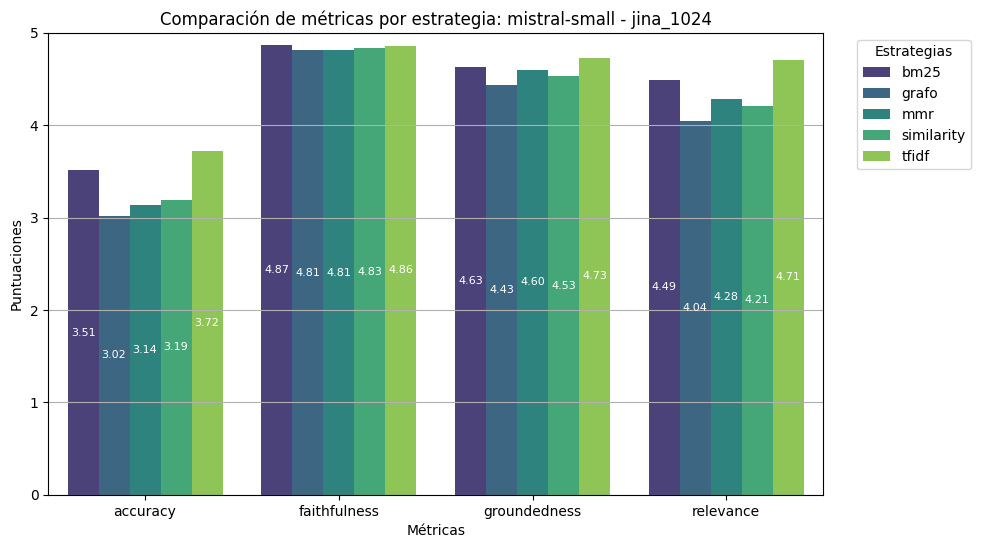
\includegraphics[width=1\textwidth]{imagenes/0129_jina_1024.png}
	    				\caption{Sin reranking}
	    			\end{subfigure}   
	    			\begin{subfigure}{.49\textwidth}
	    				\centering
	    				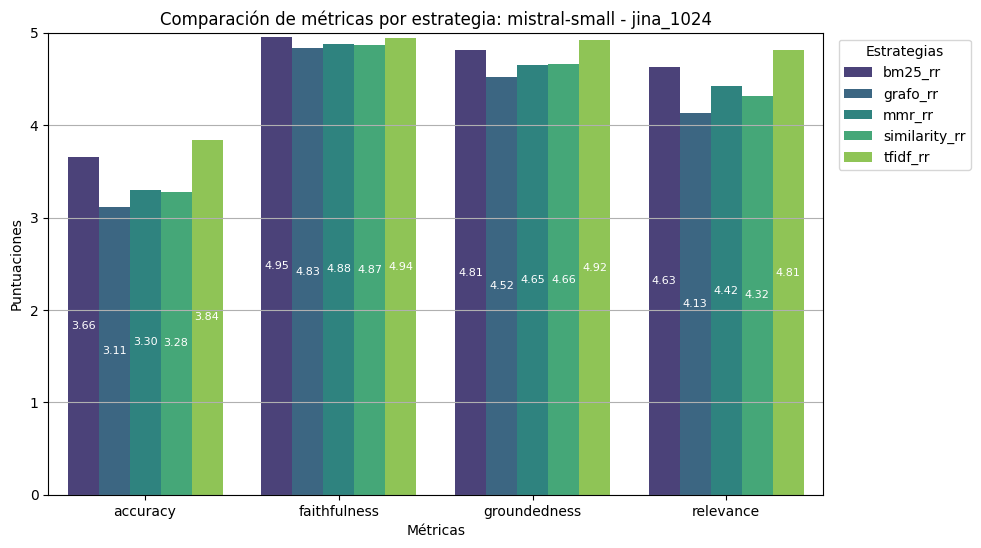
\includegraphics[width=1\textwidth]{imagenes/0129_jina_rr_1024.png}
	    				\caption{Con reranking}
	    			\end{subfigure} 			
	    			\caption{Gráfica de rendimiento del modelo Mistral Small 3.2 usando el modelo de embedding JINA y tamaños de documento 1024}
	    			\label{fig:0129_jina_1024}       
	    		\end{figure} 
	    		
	    		\begin{figure}[H]
	    			\centering
	    			\begin{subfigure}{.49\textwidth}
	    				\centering
	    				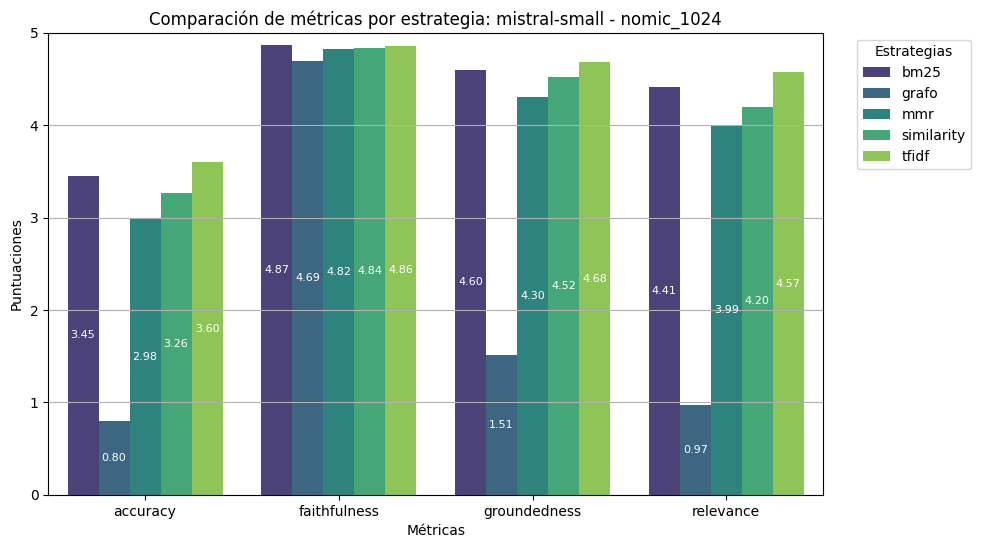
\includegraphics[width=1\textwidth]{imagenes/0130_nomic_1024.png}
	    				\caption{Sin reranking}
	    			\end{subfigure}   
	    			\begin{subfigure}{.49\textwidth}
	    				\centering
	    				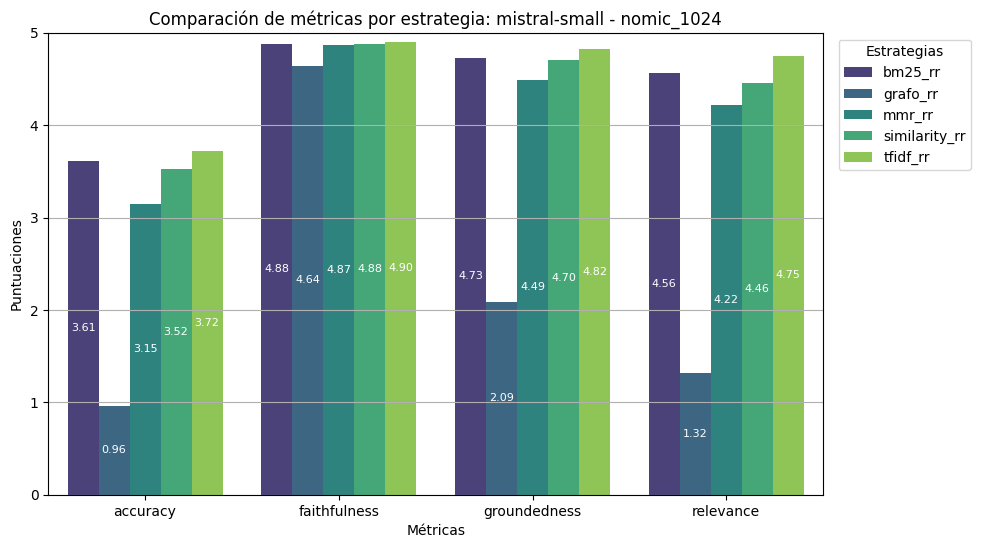
\includegraphics[width=1\textwidth]{imagenes/0130_nomic_rr_1024.png}
	    				\caption{Con reranking}
	    			\end{subfigure} 			
	    			\caption{Gráfica de rendimiento del modelo Mistral Small 3.2 usando el modelo de embedding Nomic-Embed-Text y tamaños de documento 1024}
	    			\label{fig:0130_nomic_1024}       
	    		\end{figure} 
	    		
	    		\begin{figure}[H]
	    			\centering
	    			\begin{subfigure}{.49\textwidth}
	    				\centering
	    				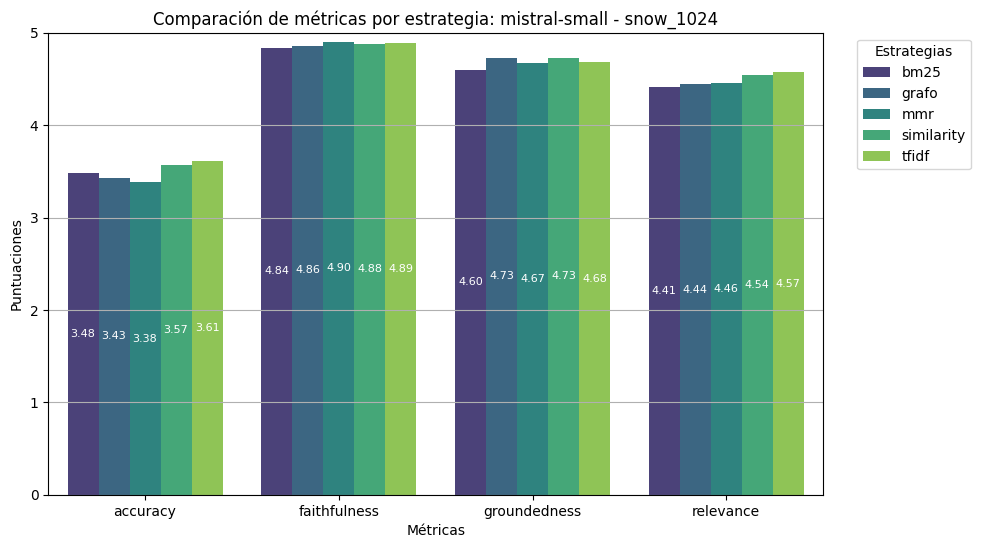
\includegraphics[width=1\textwidth]{imagenes/0131_snow_1024.png}
	    				\caption{Sin reranking}
	    			\end{subfigure}   
	    			\begin{subfigure}{.49\textwidth}
	    				\centering
	    				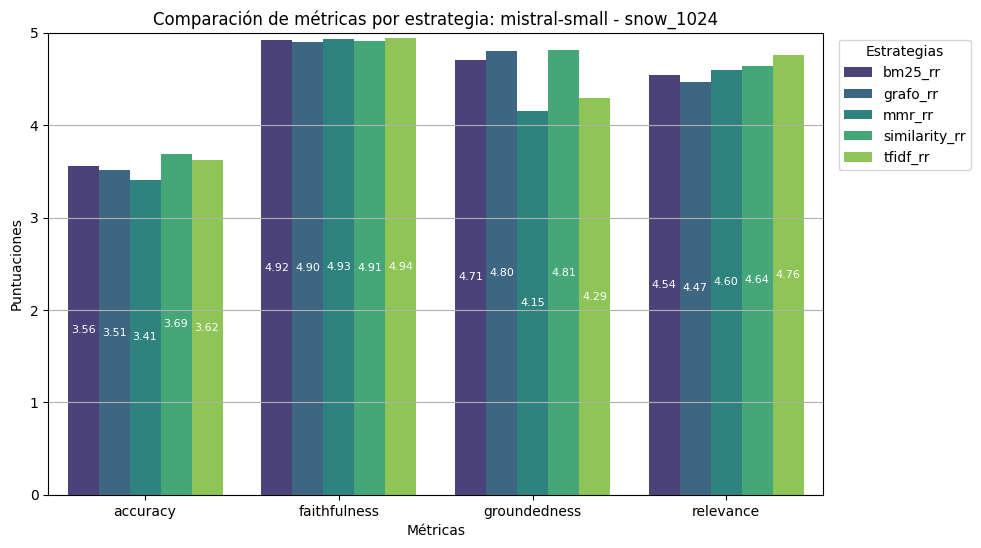
\includegraphics[width=1\textwidth]{imagenes/0131_snow_rr_1024.png}
	    				\caption{Con reranking}
	    			\end{subfigure} 			
	    			\caption{Gráfica de rendimiento del modelo Mistral Small 3.2 usando el modelo de embedding Snowflakev2 y tamaños de documento 1024}
	    			\label{fig:0131_snow_1024}       
	    		\end{figure} 	
	    		
	    	\subsubsection{Resultados usando un prompt modificado en bases de datos con tamaño de documentos 1024}
	    	
	    		En esta tanda de pruebas se hizo una modificación en el \textit{prompt} interno del sistema RAG. En este \textit{prompt} (figura  \ref{fig:0138_prompt_mejora}), se indica que debe efectuar una respuesta de forma más simple y escueta a la consulta del usuario. El \textit{prompt} por defecto se extiende demasiado en su respuesta, generando estructuras y listas que pueden afectar negativamente a la evaluación del \textit{accuracy}.    		
	    		
	    		\begin{figure}[H]
	    			\centering
	    			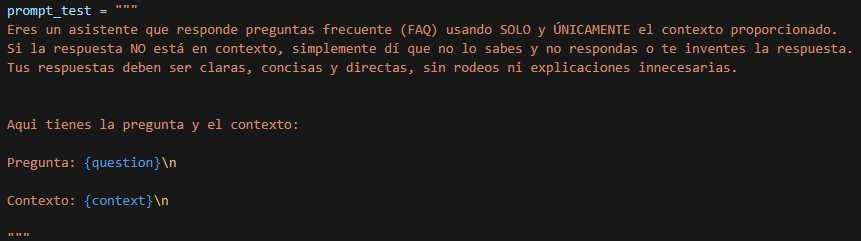
\includegraphics[width=1\textwidth]{imagenes/0138_prompt_mejora.png}
	    			\caption{Modificación hecha en el prompt}		
	    			\label{fig:0138_prompt_mejora}
	    		\end{figure} 
	    			    		
	    		\noindent Los resultados se muestran en la siguiente tabla:
	    	
	    		\newpage
		    	\begin{table}[H]
		    		\centering
		    		\tiny
		    		\begin{tblr}{
		    				row{1} = {bg=white}, 
		    				row{2-11} = {bg=yellow!20}, 
		    				row{12-21} = {bg=green!20},    				
		    				row{22-31} = {bg=blue!20}, 
		    				row{32-41} = {bg=violet!20}, 
		    				hlines,
		    				vlines,
		    			}
		    			\textbf{Embedding} & \textbf{Estrategia} & \textbf{Accuracy} & \textbf{Faithfulness} & \textbf{Groundedness} & \textbf{Relevance} \\
		    			bge-m3 & tfidf\_rr & \SetCell{bg=yellow}\textbf{3.72} & \SetCell{bg=yellow}\textbf{4.95} & \SetCell{bg=yellow}\textbf{4.4} & \SetCell{bg=yellow}\textbf{4.82} \\
		    			bge-m3 & bm25\_rr & 3.51 & 4.8 & 4.24 & 4.64 \\
		    			bge-m3 & similarity\_rr & 3.44 & 4.77 & 4.09 & 4.55 \\
		    			bge-m3 & tfidf & 3.43 & 4.83 & 4.07 & 4.67 \\
		    			bge-m3 & bm25 & 3.38 & 4.82 & 3.98 & 4.52 \\
		    			bge-m3 & mmr\_rr & 3.32 & 4.86 & 4.09 & 4.51 \\
		    			bge-m3 & grafo\_rr & 3.21 & 4.74 & 3.96 & 4.31 \\
		    			bge-m3 & similarity & 3.12 & 4.74 & 3.84 & 4.38 \\
		    			bge-m3 & mmr & 3.04 & 4.83 & 3.9 & 4.37 \\
		    			bge-m3 & grafo & 2.95 & 4.76 & 3.76 & 4.27 \\
		    			jina & tfidf\_rr & \SetCell{bg=green}\textbf{3.66} & \SetCell{bg=green}\textbf{4.92} & \SetCell{bg=green}\textbf{4.3} & \SetCell{bg=green}\textbf{4.73} \\
		    			jina & bm25\_rr & 3.55 & 4.9 & 4.26 & 4.66 \\
		    			jina & bm25 & 3.46 & 4.79 & 4.01 & 4.56 \\
		    			jina & tfidf & 3.37 & 4.81 & 3.97 & 4.57 \\
		    			jina & mmr\_rr & 3.1 & 4.87 & 3.98 & 4.41 \\
		    			jina & similarity\_rr & 3.09 & 4.77 & 3.91 & 4.37 \\
		    			jina & similarity & 2.84 & 4.72 & 3.74 & 4.22 \\
		    			jina & mmr & 2.81 & 4.88 & 3.66 & 4.26 \\
		    			jina & grafo\_rr & 2.77 & 4.53 & 3.52 & 4.12 \\
		    			jina & grafo & 2.6 & 4.48 & 3.38 & 4.06 \\
		    			nomic & tfidf\_rr & \SetCell{bg=blue!50}\textbf{3.67} & \SetCell{bg=blue!50}\textbf{4.91} & \SetCell{bg=blue!50}\textbf{4.3} & \SetCell{bg=blue!50}\textbf{4.75} \\
		    			nomic & bm25\_rr & 3.39 & 4.87 & 4.08 & 4.56 \\
		    			nomic & tfidf & 3.38 & 4.76 & 3.95 & 4.55 \\
		    			nomic & bm25 & 3.23 & 4.84 & 3.81 & 4.4 \\
		    			nomic & similarity\_rr & 3.14 & 4.75 & 3.77 & 4.36 \\
		    			nomic & mmr\_rr & 2.95 & 4.79 & 3.65 & 4.24 \\
		    			nomic & similarity & 2.9 & 4.7 & 3.44 & 4.04 \\
		    			nomic & grafo\_rr & 2.77 & 4.67 & 3.44 & 3.97 \\
		    			nomic & mmr & 2.62 & 4.85 & 3.15 & 3.99 \\
		    			nomic & grafo & 2.56 & 4.53 & 3.22 & 3.8 \\
		    			snowflake & tfidf\_rr & \SetCell{bg=violet!50}\textbf{3.65} & \SetCell{bg=violet!50}\textbf{4.92} & \SetCell{bg=violet!50}\textbf{4.27} & \SetCell{bg=violet!50}\textbf{4.75} \\
		    			snowflake & similarity\_rr & 3.53 & 4.87 & 4.24 & 4.62 \\
		    			snowflake & mmr\_rr & 3.44 & 4.89 & 4.16 & 4.62 \\
		    			snowflake & tfidf & 3.43 & 4.81 & 3.99 & 4.57 \\
		    			snowflake & similarity & 3.4 & 4.86 & 4.08 & 4.54 \\
		    			snowflake & grafo\_rr & 3.36 & 4.77 & 4.09 & 4.47 \\
		    			snowflake & bm25\_rr & 3.35 & 4.91 & 4.09 & 4.57 \\
		    			snowflake & grafo & 3.22 & 4.76 & 3.9 & 4.4 \\
		    			snowflake & bm25 & 3.21 & 4.79 & 3.79 & 4.4 \\
		    			snowflake & mmr & 3.17 & 4.95 & 3.97 & 4.51 \\
		    			
		    		\end{tblr}
		    		\caption{Resultados de Mistral Small 3.2 en embeddings 1024 de tamaño de documentos y el prompt modificado}
		    		\label{tab:result_mistral_1024++}
		    	\end{table}
		    	
		    	\noindent A la vista de los resultados obtenidos de estas pruebas, podemos asegurar que la modificación del \textit{prompt} introducida ha tenido influencia en ellos. La mejora esperada no se ha producido, y hemos tenido resultados más bajos que en el apartado anterior en todas las métricas salvo en \textit{faithfulness}.
		    	
		    	\noindent La simplificación del \textit{prompt} de la cual esperábamos mejores resultados, ha afectado negativamente a estos. El dato positivo que podemos extraer de esta batería de pruebas es que al modificar el \textit{prompt}, obtenemos una respuesta diferente del modelo de lenguaje, y por consiguiente, unos resultados distintos para nuestros test.
		    	
		    	\noindent Resultados que se pueden observar individualmente (como en los demás apartados), en las siguientes gráficas:
		    			    	
		    	\begin{figure}[H]
		    		\centering
		    		\begin{subfigure}{.49\textwidth}
		    			\centering
		    			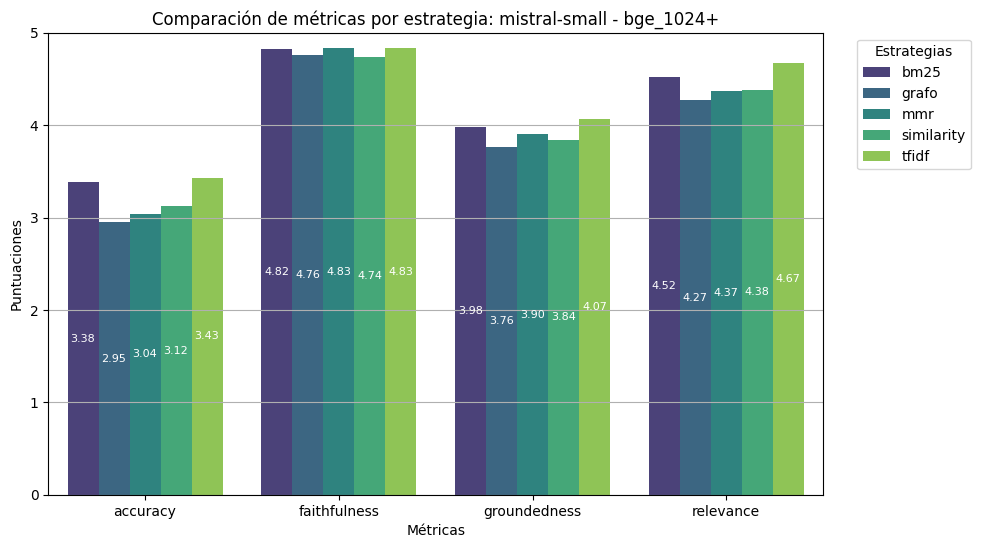
\includegraphics[width=1\textwidth]{imagenes/0132_bge+_1024.png}
		    			\caption{Sin reranking}
		    		\end{subfigure}   
		    		\begin{subfigure}{.49\textwidth}
		    			\centering
		    			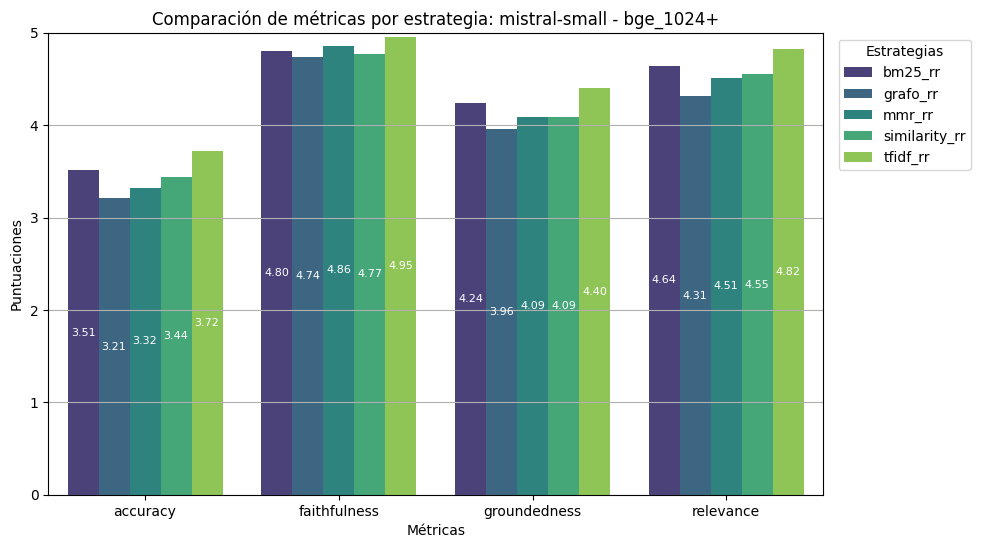
\includegraphics[width=1\textwidth]{imagenes/0132_bge+_rr_1024.png}
		    			\caption{Con reranking}
		    		\end{subfigure} 			
		    		\caption{Gráfica de rendimiento del modelo Mistral Small 3.2 usando el modelo de embedding BGE-M3, tamaños de documento 1024 y el prompt modificado}
		    		\label{fig:0132_bge+_1024}       
		    	\end{figure} 
		    	
		    	\begin{figure}[H]
		    		\centering
		    		\begin{subfigure}{.49\textwidth}
		    			\centering
		    			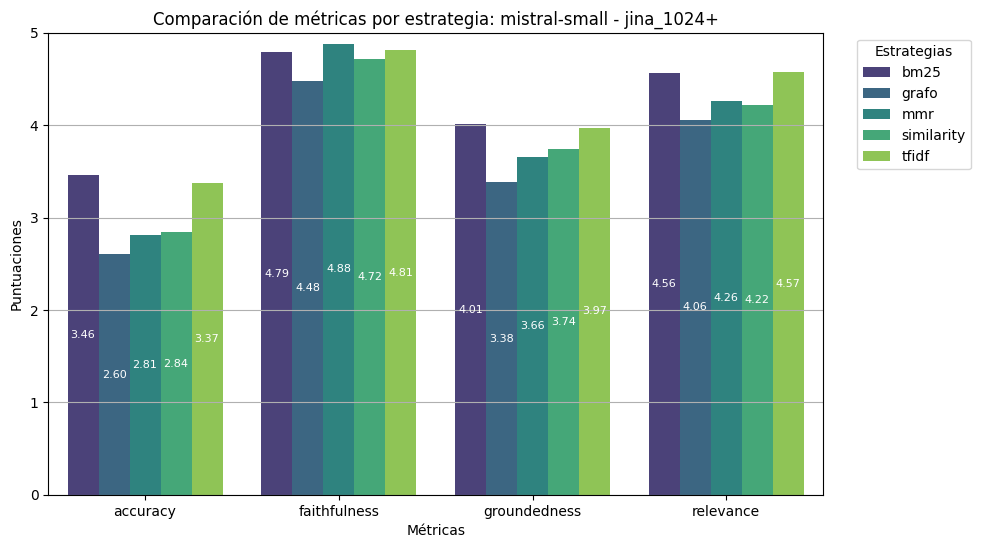
\includegraphics[width=1\textwidth]{imagenes/0133_jina+_1024.png}
		    			\caption{Sin reranking}
		    		\end{subfigure}   
		    		\begin{subfigure}{.49\textwidth}
		    			\centering
		    			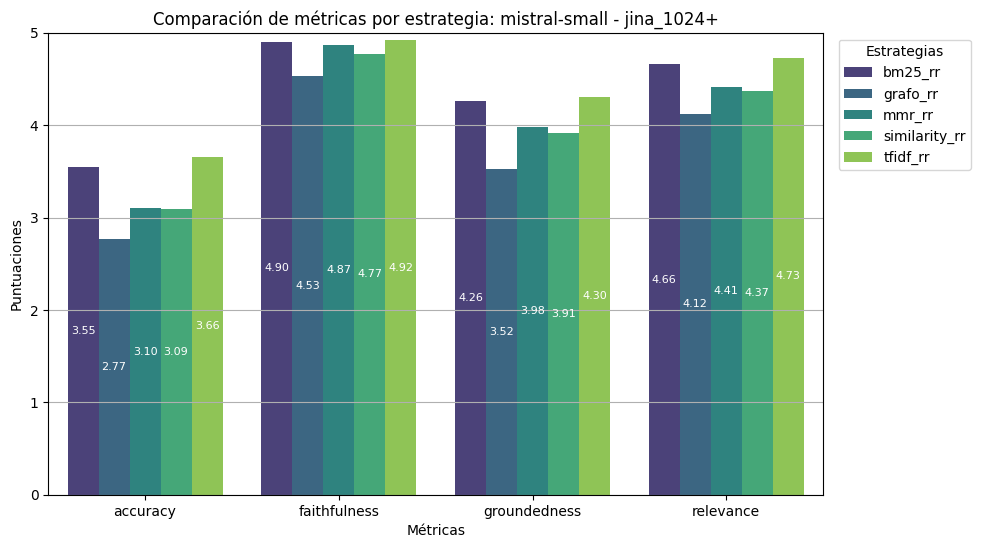
\includegraphics[width=1\textwidth]{imagenes/0133_jina+_rr_1024.png}
		    			\caption{Con reranking}
		    		\end{subfigure} 			
		    		\caption{Gráfica de rendimiento del modelo Mistral Small 3.2 usando el modelo de embedding JINA, tamaños de documento 1024 y el prompt modificado}
		    		\label{fig:0133_jina+_1024}       
		    	\end{figure} 
		    	
		    	\begin{figure}[H]
		    		\centering
		    		\begin{subfigure}{.49\textwidth}
		    			\centering
		    			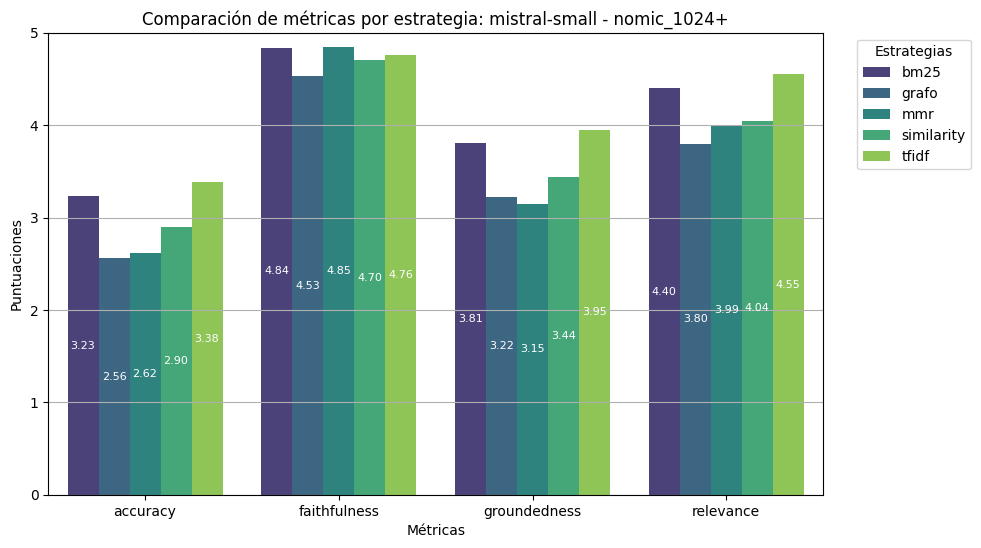
\includegraphics[width=1\textwidth]{imagenes/0134_nomic+_1024.png}
		    			\caption{Sin reranking}
		    		\end{subfigure}   
		    		\begin{subfigure}{.49\textwidth}
		    			\centering
		    			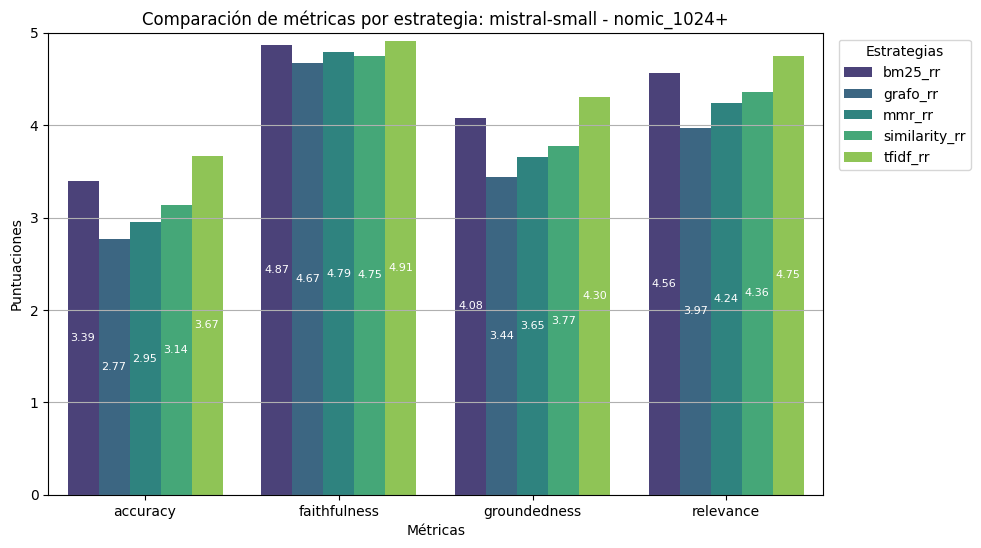
\includegraphics[width=1\textwidth]{imagenes/0134_nomic+_rr_1024.png}
		    			\caption{Con reranking}
		    		\end{subfigure} 			
		    		\caption{Gráfica de rendimiento del modelo Mistral Small 3.2 usando el modelo de embedding Nomic-Embed-Text, tamaños de documento 1024 y el prompt modificado}
		    		\label{fig:0134_nomic+_1024}       
		    	\end{figure} 
		    	
		    	\begin{figure}[H]
		    		\centering
		    		\begin{subfigure}{.49\textwidth}
		    			\centering
		    			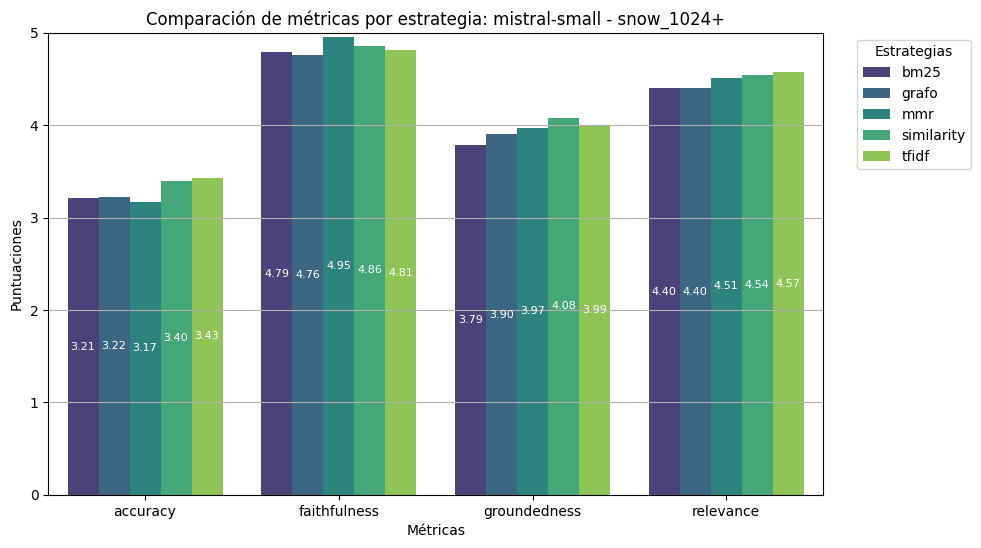
\includegraphics[width=1\textwidth]{imagenes/0135_snow+_1024.png}
		    			\caption{Sin reranking}
		    		\end{subfigure}   
		    		\begin{subfigure}{.49\textwidth}
		    			\centering
		    			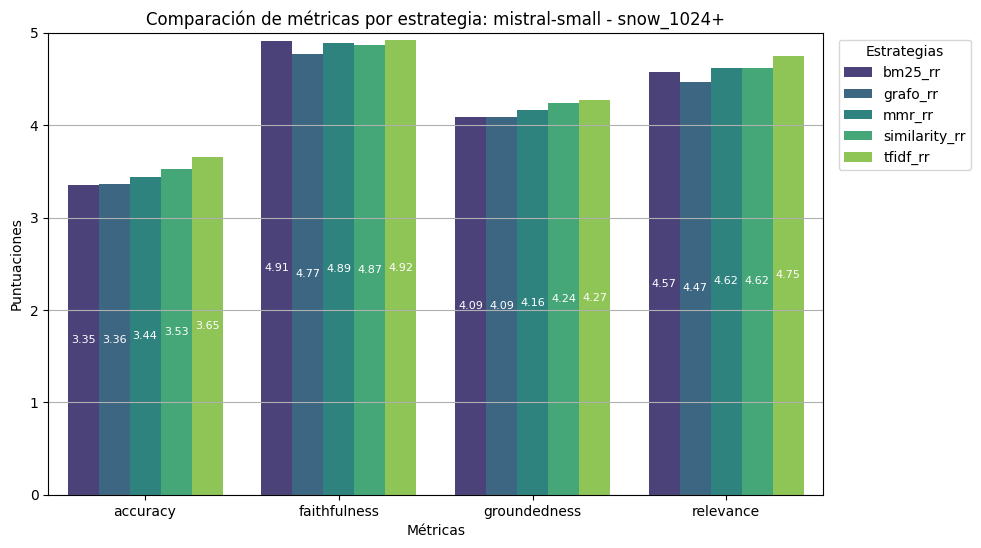
\includegraphics[width=1\textwidth]{imagenes/0135_snow+_rr_1024.png}
		    			\caption{Con reranking}
		    		\end{subfigure} 			
		    		\caption{Gráfica de rendimiento del modelo Mistral Small 3.2 usando el modelo de embedding Snowflakev2, tamaños de documento 1024 y el prompt modificado}
		    		\label{fig:0135_snow+_1024}       
		    	\end{figure} 	
		    	  	
    	\subsection{Resultados de Llama 3.2}
    	
    		\textit{Llama 3.2} es el modelo usado para realizar estas pruebas de forma local. Este modelo es el más modesto de los utilizados en el proyecto, contando solo con 3 billones (ingleses) de parámetros. Debido a esto, se espera recibir unos resultados peores a los anteriores mostrados.
    		
    		\noindent Otro factor importante derivado del método de ejecución de este modelo es que, al ser ejecutado localmente, consume bastante tiempo en generar una respuesta. Al depender de la configuración de la máquina donde se use, si esta no cumple con los requisitos necesarios los tiempos de respuesta se alargan considerablemente. En nuestro caso, al no disponer de una tarjeta gráfica \textit{nvidia}, sufrimos esta consecuencia.
    		
    		\noindent Para mitigar la tardanza en el tiempo de respuesta, se planteó usar un 10\% del conjunto de preguntas (unas 30) y extrapolar los resultados. Dichos resultados se obtuvieron en una media de 3 horas y 20 minutos para cada prueba, empleándose alrededor de unas 16 horas y 40 minutos para realizar las pruebas en un solo embedding con la suma de todas las estrategias de búsqueda.
    		
    		\noindent Los resultados obtenidos para un solo embedding se muestran en la siguiente tabla:
    		
    		\begin{table}[H]
    			\centering
    			\tiny
    			\begin{tblr}{
    					row{1} = {bg=white}, 
    					row{2-11} ={bg=green!20},    
    					hlines,
    					vlines,
    				}
    				\textbf{Embedding} & \textbf{Estrategia} & \textbf{Accuracy} & \textbf{Faithfulness} & \textbf{Groundedness} & \textbf{Relevance} \\
    				jina & similarity\_rr & \SetCell{bg=green}\textbf{3.08} & 4.17 & \SetCell{bg=green}\textbf{3.75} & 4.25 \\
    				jina & grafo & 2.94 & 4.29 & 3.18 & 4.18 \\
    				jina & similarity & 2.76 & 3.94 & 3.41 & 4.24 \\
    				jina & tfidf\_rr & 2.5 & \SetCell{bg=green}\textbf{4.5} & 3.33 & \SetCell{bg=green}\textbf{4.67} \\
    				jina & tfidf & 2.4 & 4.0 & 3.47 & 4.33 \\
    				jina & bm25\_rr & 2.36 & 4.18 & 3.0 & 4.36 \\
    				jina & grafo\_rr & 2.3 & 4.4 & 3.2 & 4.6 \\
    				jina & mmr & 2.29 & 4.29 & 3.43 & 3.86 \\
    				jina & mmr\_rr & 1.8 & 4.1 & 3.4 & 3.9 \\
    				jina & bm25 & 1.76 & 3.94 & 3.0 & 4.53 \\
    				
    			\end{tblr}
    			\caption{Resultados de Llama 3.2 en embeddings 1024 de tamaño de documentos}
    			\label{tab:result_llama}
    		\end{table}
    		
    		\noindent Y como se esperaba, se obtienen los peores resultados en todas las métricas. Destaca la pobre puntuación obtenida en el \textit{accuracy} en la mayoría de los agentes, algunos no llegan a superar el 50\%. Siendo la mejor puntuación de esta, casi 8 décimas peor que el mejor modelo, esta claro que no es un modelo aconsejable para el uso. 
    		
    		\noindent Aunque las demás métricas consiguen resultados más o menos decentes, siguen estando muy por debajo de las mejores puntuaciones obtenidas.
    		
    		\noindent No se ha decidido usar otro modelo de embedding por los malos resultados obtenidos usando \textit{JINA}, el mejor modelo en comparación vistas las otras tablas de pruebas.
    		
    		\noindent En las siguientes figuras, se muestra de forma gráfica los resultados presentes en la tabla \ref{tab:result_llama}.
    		
    		\begin{figure}[H]
    			\centering
    			\begin{subfigure}{.49\textwidth}
    				\centering
    				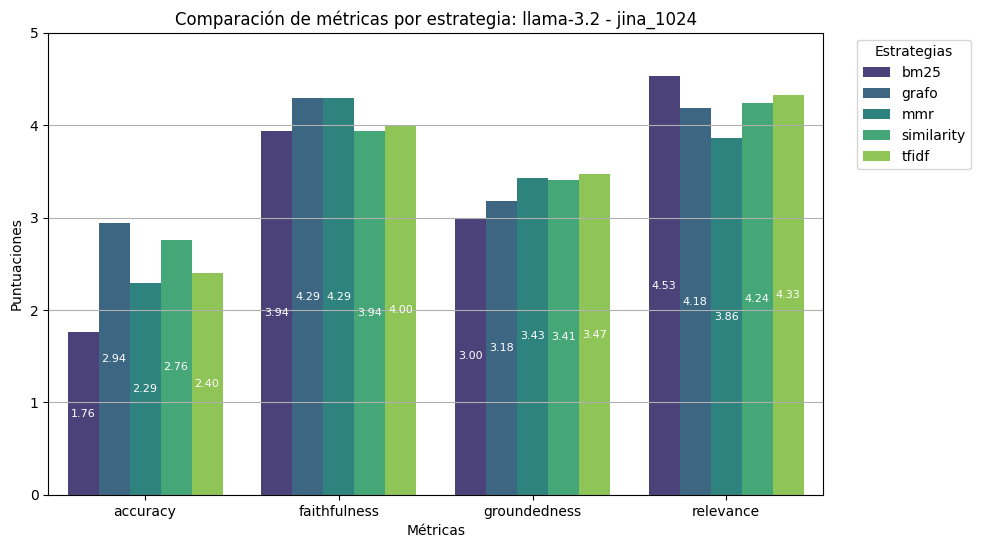
\includegraphics[width=1\textwidth]{imagenes/0136_llama_jina.png}
    				\caption{Sin reranking}
    			\end{subfigure}   
    			\begin{subfigure}{.49\textwidth}
    				\centering
    				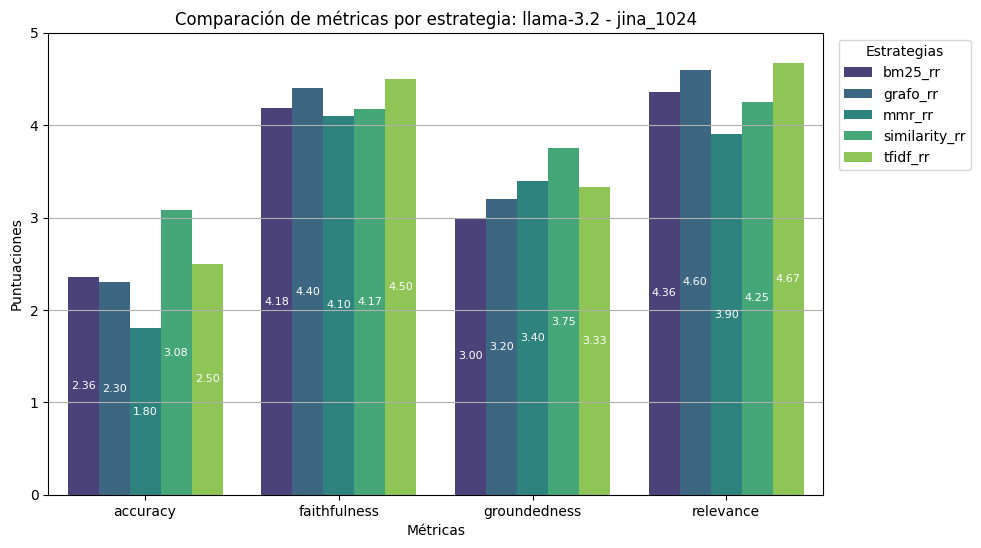
\includegraphics[width=1\textwidth]{imagenes/0136_llama_jina_rr.png}
    				\caption{Con reranking}
    			\end{subfigure} 			
    			\caption{Gráfica de rendimiento del modelo Llama 3.2 usando el modelo de embedding Jina y tamaños de documento 1024}
    			\label{fig:0136_llama_jina}       
    		\end{figure} 
    	
    	\subsection{Resultados de GPT-4.1}
    	
    		El modelo \textit{GPT-4.1} es el último usado en las pruebas definidas en nuestro proyecto. Este modelo perteneciente a \textit{OpenAI} es de pago, por lo que hay que controlar el uso que le pedimos a esta plataforma si no queremos gastar mucho dinero. Por este motivo se redujo el conjunto de pruebas a un 25\% del total (75 preguntas) para después extrapolar los resultados conseguidos.
    		
    		\noindent A su vez, el modelo de embedding utilizado para las pruebas también comparte plataforma con este modelo de lenguaje. Se optó por probar ambos, para medir el rendimiento de los modelos de pago en comparación al resto. El modelo de embedding (\textit{text-embedding-3-small}) fue configurado para usar documentos de tamaño 1024.
    		
    		\noindent El tiempo para obtener los resultados fue de 40 minutos por modelo de embedding. Teniendo en cuenta que obtenemos los resultados sin y con \textit{reranking} en la misma prueba, se produjeron cinco ejecuciones en un total de dos horas y media, con un costo aproximado de 15 dólares.
    		
    		\noindent\textbf{Nota:} Cada consulta hecha generaba alrededor de 3000 tokens, y su coste era de 0,01\$.
    		
    		\noindent Los resultados de las pruebas son los mostrados en la siguiente tabla:
    		
    		\begin{table}[H]
    			\centering
    			\tiny
    			\begin{tblr}{
    					row{1} = {bg=white}, 
    					row{2-11} ={bg=violet!20},    
    					hlines,
    					vlines,
    				}
    				\textbf{Embedding} & \textbf{Estrategia} & \textbf{Accuracy} & \textbf{Faithfulness} & \textbf{Groundedness} & \textbf{Relevance} \\
    				text-embedding-3-small & tfidf & \SetCell{bg=violet!50}\textbf{4.32} & \SetCell{bg=violet!50}\textbf{4.95} & 4.91 & 4.68 \\
    				text-embedding-3-small & tfidf\_rr & 4.27 & 4.92 & \SetCell{bg=violet!50}\textbf{4.96} & \SetCell{bg=violet!50}\textbf{4.75} \\
    				text-embedding-3-small & similarity\_rr & 3.96 & 4.89 & 4.88 & 4.41 \\
    				text-embedding-3-small & similarity & 3.95 & 4.88 & 4.89 & 4.49 \\
    				text-embedding-3-small & mmr\_rr & 3.92 & 4.89 & 4.88 & 4.59 \\
    				text-embedding-3-small & bm25 & 3.83 & 4.91 & 4.88 & 4.45 \\
    				text-embedding-3-small & bm25\_rr & 3.83 & 4.92 & 4.95 & 4.41 \\
    				text-embedding-3-small & grafo\_rr & 3.68 & 4.91 & 4.85 & 4.19 \\
    				text-embedding-3-small & grafo & 3.67 & 4.87 & 4.81 & 4.17 \\
    				text-embedding-3-small & mmr & 3.6 & 4.87 & 4.81 & 4.28 \\
    			\end{tblr}
    			\caption{Resultados de GPT-4.1 en embeddings 1024 de tamaño de documentos}
    			\label{tab:result_gpt}
    		\end{table}
    		
    		\noindent Como se puede apreciar en la tabla anterior, los resultados obtenidos son los mejores obtenidos hasta ahora, con la única excepción de la métrica de relevancia. 
    		
    		\noindent En el caso del \textit{accuracy}, las estrategias \textit{TF-IDF} sin y con \textit{reranking} superan los 4.25 de puntuación, lo cual indica una respuesta muy parecida a la esperada. Para las demás estrategias, el \textit{accuracy} siempre supera a la mejor obtenida anteriormente. 
    		
    		\noindent Las métricas \textit{faithfulness} y \textit{groundedness} se mantienen muy altas, rozando el 5 en las mejores y siempre superando la puntuación mínima de 4.8. Es una buena manera de saber que, con estos modelos se utiliza muy bien el contexto recuperado para generar las respuestas.
    		
    		\noindent En cuanto a la relevancia, aún no siendo el valor más alto obtenido en estas pruebas, el mejor conseguido sigue manteniendo una puntuación muy alta (4.75). A excepción de algunas estrategias, las puntuaciones obtenidas en esta métrica son generalmente muy altas.
    		
    		\noindent En las siguientes figuras, podemos ver el contenido de la tabla \ref{tab:result_gpt} de forma gráfica.
    		
    		\begin{figure}[H]
    			\centering
    			\begin{subfigure}{.49\textwidth}
    				\centering
    				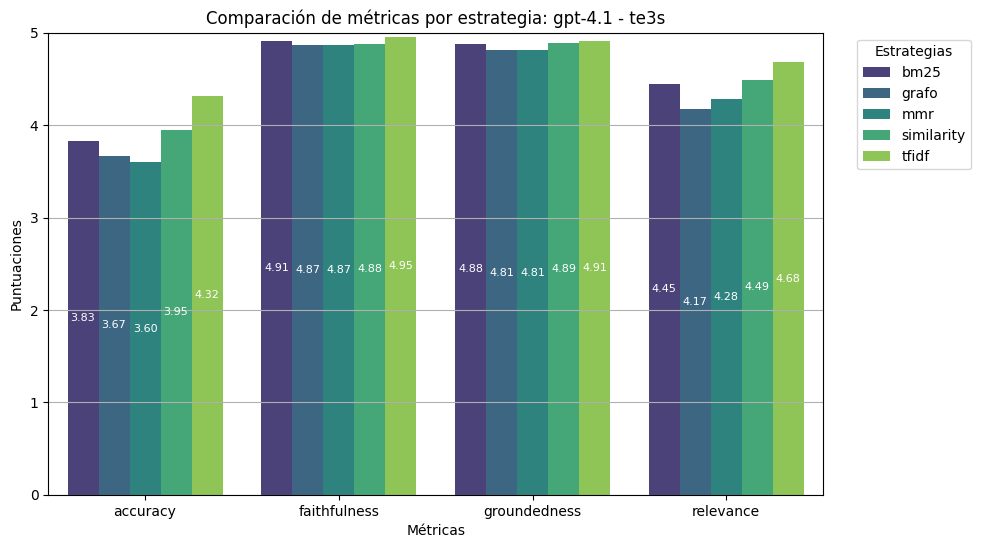
\includegraphics[width=1\textwidth]{imagenes/0137_gpt_te3s.png}
    				\caption{Sin reranking}
    			\end{subfigure}   
    			\begin{subfigure}{.49\textwidth}
    				\centering
    				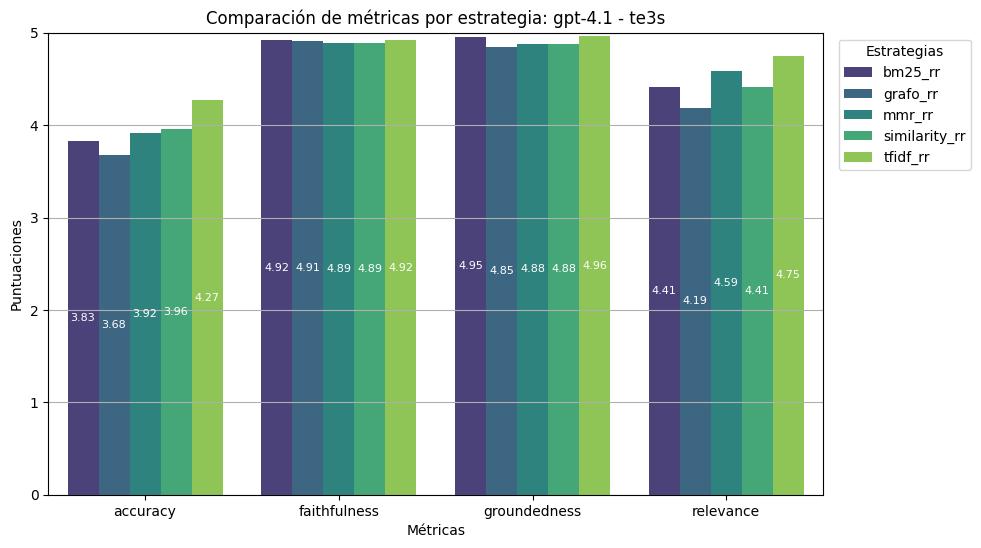
\includegraphics[width=1\textwidth]{imagenes/0137_gpt_te3s_rr.png}
    				\caption{Con reranking}
    			\end{subfigure} 			
    			\caption{Gráfica de rendimiento del modelo GPT-4.1 usando el modelo de embedding text-embedding-3-small y tamaños de documento 1024}
    			\label{fig:0137_gpt_te3s}       
    		\end{figure} 
    		
   	\section{Conclusión sobre los resultados}
   	
   		Tras realizar las pruebas y, habiendo consultado los resultados; podemos concluir aportando el conocimiento adquirido de estos. Para ello, vamos a responder una lista de preguntas relacionadas con el rendimiento del RAG ante cambios o modificaciones en su configuración. Y como colofón, explicaremos las deducciones finales obtenidas sobre los resultados.
   		
   		%\subsection{Preguntas sobre los resultados}
   		
	   		\noindent\textbf{¿Cómo afecta el tamaño del LLM a la calidad de la respuesta en un sistema RAG?} Los modelos de lenguaje más grandes (con mayor número de parámetros) obtienen mejores resultados. Los resultados obtenidos por \textit{Llama 3.2} (tabla \ref{tab:result_llama}) son inferiores a los otros dos modelos de lenguaje (tablas \ref{tab:result_mistral_1024} y \ref{tab:result_gpt}). Esto se debe al tamaño de los modelos, Llama 3.2 (3B) es mucho más pequeño que \textit{Mistral Small 3.2} (24B) y \textit{GPT-4.1} (desconocido, aunque sabemos que la versión GPT3 cuenta con 175B de parámetros). Por lo tanto, podemos asegurar que conseguiremos mejores respuestas con modelos más grandes.
	   		
	   		\noindent\textbf{¿Pueden diferencias sutiles en el prompt afectar significativamente la alineación de la recuperación y la generación?} En nuestro caso, solo afecta a la generación de respuesta, ya que la recuperación no se utiliza un \textit{prompt} (recupera documentos relevantes a la consulta). En la prueba realizada modificando el \textit{prompt} (tabla \ref{tab:result_mistral_1024++}), pedimos una respuesta más simple y escueta, y los resultados consecuente fueron peores a los conseguidos anteriormente. Debido a esto, concluimos que el \textit{prompt} usado por defecto es mejor generando una respuesta más parecida a la esperada y, que la modificación de este influye en los resultados.
	   		
	   		\noindent\textbf{¿Cómo impacta el tamaño del fragmento de documento recuperado en la calidad de la respuesta?} Hemos comprobado este factor en las dos primeras tandas de pruebas (tablas \ref{tab:result_mistral_512} y \ref{tab:result_mistral_1024}). Los resultados obtenidos muestran que un tamaño mayor es mejor para generar una respuesta. Así que, podemos decir que la respuesta generada se ve favorecida si dispone de documentos recuperados con un mayor tamaño de contexto.
	   		
	   		\noindent\textbf{¿Cómo impacta el tamaño de la base de conocimiento en el rendimiento general?} Hemos trabajado con bases de conocimiento que oscilaban entre 45MB y 65MB, por lo que no hemos apreciado diferencias considerables en el tiempo de recuperación de documentos. Este tiempo era casi inmediato para todas las bases de conocimiento, al contrario que el tiempo de creación de la bases de conocimiento, variando entre los 12 minutos (figura \ref{fig:0079_success1}) y 35 minutos (figura \ref{fig:0079_success2}) para las bases de datos locales, y los 40 segundos para el embedding \textit{text-embedding-3-small} (figura \ref{fig:0099_te3s-embed}), que opera vía API desde \textit{OpenAI}. Así pues, tenemos dos opciones: si valoramos más el tiempo de recuperación, la elección es una base local gratuita dado a su nula diferencia; en cambio, si valoramos más el tiempo de creación, los métodos de pago son muy superiores.   		
	   		    		
	   		\noindent\textbf{¿Afecta la incorporación de documentos multilingües a las respuestas del sistema RAG?} En nuestro caso, al manejar siempre documentos escritos en español (BOE), no hemos podido comprobar este factor. Podemos responder a esta pregunta diciendo que los modelos de embedding que mejor se han comportado con nuestra base de conocimiento son los multilingües, especialmente \textit{JINA} (entrenado en español e inglés) y \textit{text-embedding-3-small} (de pago).
	   		
	   		\noindent\textbf{¿El centrarse en unas pocas oraciones recuperadas agudiza las respuestas de RAG?} Negativo, hemos demostrado en las pruebas que se obtienen mejores resultados al aumentar el tamaño de contexto de los documentos. En cambio, si la pregunta se refiere a reducir los documentos recuperados para mejorar la respuesta, podemos decir que el filtrado de ellos realizado por el \textit{reranker} mejora siempre las puntuaciones asignadas por los agentes.
   		
		%\subsection{Deducciones finales}
		
			En resumen, los resultados muestran dos estrategias claras que podemos usar para recomendar un sistema u otro, basándonos sólo en el presupuesto que estemos dispuestos a emplear como factor determinante.
			
			\noindent La primera estrategia es la ofrecida por la combinación de los modelos de pago (embedding y generación), ya que siempre obtienen los mejores resultados. Recordemos que el coste de la consulta era de alrededor de 0,01\$, un precio asequible pero que se puede disparar ante una gran demanda. 			
			   			
	   		\noindent En cambio la segunda estrategia es, usar el modelo de lenguaje \textit{Mistral Small 3.2} y embeddings locales. A la vista de los resultados, el uso de este modelo junto a una base vectorial \textit{JINA} puede ser bastante competente. Como se ha comentado, el embedding \textit{JINA} es un modelo bilingüe español-inglés, por lo que es ideal para nuestra base de conocimiento.
   			
   			\noindent En cuanto a la estrategia de búsqueda, los mejores resultados los obtienen los métodos tradicionales: \textit{TF-IDF}, \textit{BM25} y similaridad coseno. Destacando la mayoría de veces \textit{TF-IDF} sobre el resto.

\endgroup

\begingroup
\titleformat{\chapter}[block]
{\normalfont\Huge\bfseries\centering} 
{Capítulo \thechapter} 
{0.5em}
{: \LARGE}
[\vspace{1em}\titlerule]

\titlespacing*{\chapter}{0pt}{-60pt}{40pt}

\chapter{Conclusiones y Líneas Futuras}
\label{cap:5_end}

	En este capítulo presentamos las conclusiones alcanzadas tras haber realizado este proyecto. Asimismo, finalizaremos explicando posibles mejoras y vías de desarrollo que podría seguir el proyecto si decidimos realizar futuras expansiones.
	
	\section{Conclusiones}
	
		Inicialmente este proyecto fue planeado como una continuación de mi Trabajo de Fin de Grado y de mi experiencia como investigador de la UGR especializado en el desarrollo de sistemas conversacionales. En él, aplicaría mis conocimientos adquiridos sobre la plataforma RASA. 
		
		\noindent Sin embargo, este es el ejemplo más claro de lo rápido que cambian los tiempos, sobre todo en el ámbito de la informática. En apenas unos años, hemos visto el resurgimiento de los modelos de lenguaje, que llevados de la mano de nuevos paradigmas de diseño, han dejado obsoletos a los enfoques más tradicionales. Ya nadie va a perder el tiempo entrenando y desarrollando un modelo específico cuando de una manera inmediata, podemos recibir una respuesta a través de las plataformas donde están alojados estos nuevos modelos.
		
		\noindent Así pues, durante la realización de este proyecto tuvimos que dejar todo lo aprendido y apostar por este \textit{nuevo} enfoque. Lo cual nos llevó a aprender nuevos frameworks de diseño y a usar diferentes modelos tanto de lenguaje como de vectorización (embedding), dado el carácter del proyecto. Además de utilizar plataformas modernas de pago por uso (servicios cloud), utilizadas hoy en día por la mayoría de las compañías del sector TIC.
		
		\noindent En este sentido, el desarrollo de la aplicación fue prácticamente guiado a través de la gran número de tutoriales o de la magnífica documentación oficial que poseen estas nuevas tecnologías. \textit{LangChain} -una de las librerías más usadas-, permite integraciones con multitud de aplicaciones, lo que ocasionó una rápida implementación y adaptación del código, y conexión con las principales plataformas que sirven los distintos modelos de lenguaje. 
		
		\noindent En cuanto a la interfaz, más de lo mismo. \textit{Streamlit} utiliza un enfoque más moderno que inyecta código \textit{Python} para crear una interfaz web. Como ya hemos comentado, con \textit{Streamlit} podemos acceder a bastantes elementos de personalización (inputs, selectbox, radio buttons) propios de HTML desde el \textit{backend}, lo que personalmente me ayudo al estar más familiarizado con este tipo de desarrollos.
		
		\noindent Respecto a los resultados, tenemos varias conclusiones que podemos ver en la siguiente lista:
		
		\begin{enumerate}
			\item Hemos demostrado la superioridad del enfoque \textit{Advanced RAG} en todos los casos de comparación, exceptuando la prueba hecha con \textit{OpenAI} (tabla \ref{tab:result_gpt}). El filtrado de documentos realizado tras la primera recuperación ofrecido por el modelo encargado de hacer el \textit{reranking} \cite{0036_bge_reranker}, mejora la calidad de las respuestas de manera ostensible.
			\item El modelo de embedding también es importante. Aunque los modelos usados en el proyecto son todos multilingües, \textit{JINA} \cite{0027_jina} esta especializado en nuestro idioma (bilingüe español-inglés). A la prueba de los resultados, es el más recomendable para su uso en este contexto.
			\item \textit{TF-IDF} se muestra como la estrategia de búsqueda más solida en las pruebas realizadas, seguida de \textit{BM25} y la búsqueda por similaridad coseno en la mayoría de los casos.			
		\end{enumerate}
		
		\noindent Para finalizar con los resultados, hay un motivo por el cual hemos realizado la mayoría de las pruebas con el modelo de lenguaje \textit{Mistral Small 3.2} \cite{0038_mistralsmall32}. Este modelo es gratuito y de libre acceso a través de la API provista por \textit{Mistral} en su página web. La calidad y velocidad de respuesta que obtuvimos, hizo posible la realización de todas las pruebas que necesitábamos. Por otro lado, el modelo local usado \textit{Llama3.2} \cite{0037_llama32}, era mucho más lento en la obtención de respuestas (aún usando un conjunto muy reducido) y la calidad de ellas no era muy buena (tabla \ref{tab:result_llama}), por lo que descartamos hacer más. Y si miramos al modelo de \textit{OpenAI}, los motivos fueron dos: primero económico y segundo porque en la primera tanda de pruebas consiguió mejores resultados que todas las anteriores. Así pues, cumplimos el mini-objetivo de demostrar que un modelo más grande mejora los resultados y finalizamos las pruebas.
		
		\noindent En resumen, pienso que este Trabajo de Fin de Máster ha cambiado mi percepción como desarrollador de sistemas conversacionales. Desarrollar con RASA era más complicado en codificación y lento en entreno, y aunque los resultados eran buenos, siempre estaba el riesgo de que no tuviese consistencia en la respuesta, ya sea al usar palabras distintas a las usadas en el entreno o porque el propio modelo se salte pasos. Con el nuevo enfoque empleado en el proyecto, hemos tenido un desarrollo rápido y versátil, y me ha aportado algo de la experiencia en estos nuevos paradigmas que tanto se busca en entornos profesionales.
		
		\noindent Y sobre el tema del proyecto, este trabajo se inserta en un ámbito en el que ya han surgido aplicaciones orientadas a dar respuesta a la DANA, como \textit{Ajuda Dana} y \textit{TuCocheDana}. Asimismo, proyectos como \textit{Justicio} han mostrado cómo el enfoque RAG puede transformar la manera en que accedemos e interpretamos el BOE. En este contexto, nuestro TFM presenta una combinación ambos enfoques, con el propósito de ayudar a la ciudadanía a encontrar información oficial, veraz y comprensible en un momento de necesidad.
		
		\noindent En definitiva, este trabajo refleja cómo el uso responsable de la inteligencia artificial puede convertirse en una herramienta clave para acercar la documentación oficial a la ciudadanía. Si se orienta hacia la transparencia, la accesibilidad y la veracidad, la IA no solo facilita la gestión de la información en situaciones críticas como la DANA, sino que también contribuye a construir un futuro mejor informado y más participativo.
	
	\section{Líneas futuras}
	
		En este último apartado, comentaremos posibles mejoras que pueden añadirse al proyecto que, ya sea por falta de tiempo o recursos, no se han efectuado. Estas ideas han ido apareciendo durante la realización del proyecto.
		
		\noindent En la interfaz han surgido varias ideas de mejora en la personalización tanto  de la consulta como de la creación o actualización de la fuente de conocimiento. Aspectos como poder seleccionar la base de datos a la que queremos hacer la consulta, o poder modificar la configuración de los documentos o su embedding, ayudan a que la aplicación sea más manejable para un usuario no experto y no obliga a cambiar estos datos en el código como se hace ahora.
	
		\noindent Igualmente, se planteó añadir una página para realizar los test del sistema RAG en la interfaz. Esta parte se añadiría a una página nueva, en la que se podrían editar los siguientes parámetros:
		
		\begin{itemize}
			\item \textbf{Dataset de preguntas:} Manteniendo el formato visto en el apartado \ref{sec:4_gen_dataset}, se puede usar el conjunto de preguntas que deseemos. También se puede añadir un parámetro numérico para controlar el porcentaje o fragmento de preguntas a usar en el test.
			\item \textbf{Botones de selección de:} base de datos, estrategia de búsqueda, reranking, embedding y LLM.
		\end{itemize}
		
		\noindent Los resultados serían mostrados dinámicamente en la interfaz, ya que \textit{Streamlit} proporciona elementos como una barra de progreso que podemos actualizar fácilmente usando el número de preguntas. Pienso que sería una actualización muy interesante, la cual no se ha realizado por falta de tiempo.
		
		\noindent Con relación a los test de nuestro RAG, aunque hemos cubierto bastantes posibilidades, no hemos comprobado los resultados que pudiésemos haber obtenido al probar el aprendizaje en contexto (\textit{In-Context-Learning})que mencionamos en el Estado del Arte. Añadiendo al \textit{prompt} un mínimo porcentaje del conjunto de preguntas, haría que el LLM reconociese el formato y, supuestamente, respondiese mejor a la consulta del usuario.
		
		\noindent Finalmente, aunque el proyecto es totalmente funcional, necesita los requerimientos ubicados en el repositorio \cite{0045_repo}. Este factor no sería necesario se estuviese contenerizado ya sea en \textit{docker} u otra plataforma parecida. De esta manera funcionaria en cualquier sistema bajo cualquier plataforma gestora de contenedores. Queda como futura actualización.   

\endgroup

% \nocite{*}
% \bibliography{bibliografia/bibliografia}\addcontentsline{toc}{chapter}{Bibliografía}
% \bibliographystyle{miunsrturl}

%\bibliographystyle{unsrt}  
%\bibliography{bibliografia/bibliografia}
\printbibliography


%
%\appendix
%\input{apendices/manual_usuario/manual_usuario}
%%\input{apendices/paper/paper}
%\input{glosario/entradas_glosario}
% \addcontentsline{toc}{chapter}{Glosario}
% \printglossary
% \chapter*{}
% \thispagestyle{empty}

\end{document}
